\ifcase0  % choose 0=slides, 1=article, 2=refart
	 \documentclass[ignorenonframetext,12pt]{beamer}
	 \geometry{paper=a6paper,landscape}
\or\documentclass[a4paper,11pt]{article}
	 \usepackage{url,beamerarticle}
\or\documentclass[a4paper,11pt]{refart}
	 \let\example\relax
	 \usepackage{url,beamerarticle}
\fi

\ifcase0  % choose a theme like these
%\usetheme{Montpellier}% I recommend
	 \usetheme{default}% I recommend
\or\usetheme{Singapore}
\or\usetheme{Szeged}
\or\usetheme{Boadilla}
\or\usetheme{Pittsburgh}
\or\usetheme{Madrid}
\or\usetheme{Warsaw} % common choice, but often poor
\fi

\usepackage[utf8]{inputenc}%para acentos en español
\usepackage{graphicx,pgfplots,parskip}
\usepackage{siunitx}
\graphicspath{{media/}}
\usepackage{xcolor}
\usepackage[percent]{overpic}

\title{Microelectrónica y técnicas avanzadas de procesamiento digital con
aplicaciones en micro-resonadores superconductores multipíxeles}
\subtitle{\alert{Charla de avance}}
\author{Ing. L. Horacio Arnaldi\\
Laboratorio Detecci\'on de Part\'iculas y Radiaci\'on\\
CAB-IB}
\date{12 de Diciembre, 2019}

\begin{document}

\begin{frame}
				\maketitle
\end{frame}

\begin{abstract}
				This abstract, being outside the frame environment, does not appear in
				the presentation.  Your outline will be the basis for a couple of
				sentences of talk for each of the following questions:
				\begin{itemize}
								\item What was done?
								\item Why do it?
								\item What were the results?
								\item What do the results mean in theory and/or practise?
								\item What is the reader's benefit?
								\item How can the readers use this information for themselves? 
				\end{itemize}
\end{abstract}

%\begin{frame}{Outline}
%				\tableofcontents
%\end{frame}

%------------------------------------------------------------------------------
\section{Motivación}
\begin{frame}{Motivación}
				\begin{itemize}
								\item ¿Qué me motiva a hacer esto?
								\item Desarrollar un grupo de estudios/mediciones en RF a bajas
												temperaturas
								\item Desarrollo de nuevas herramientas/instrumentos potenciados
												por el uso de dispositivos lógicos programables (FPGA,
												GPU, CPU, etc.) de última generación
								\item ¿Por qué lo hago?
								\item En los últimos años se viene trabajando fuertemente en
												detectores de baja temperatura y altas frecuencias
								\item ¿Qué beneficios obtengo/obtenemos?
								\item Creación de grupos inter-disciplinarios para el estudio de
												fenómenos poco conocidos/estudiados en el CAB
								\item ¿Qué grupos integro/se formaron con esto?
								\item Grupo de BT, Nano-Microelectrónica, PyC
								\item 
				\end{itemize}

\end{frame}

\begin{frame}{Motivación}
				\framesubtitle{Estudios del CMB}
												\only<1>{\includegraphics[width=0.4\textwidth]{c1_cmb_map}}
												\only<1>{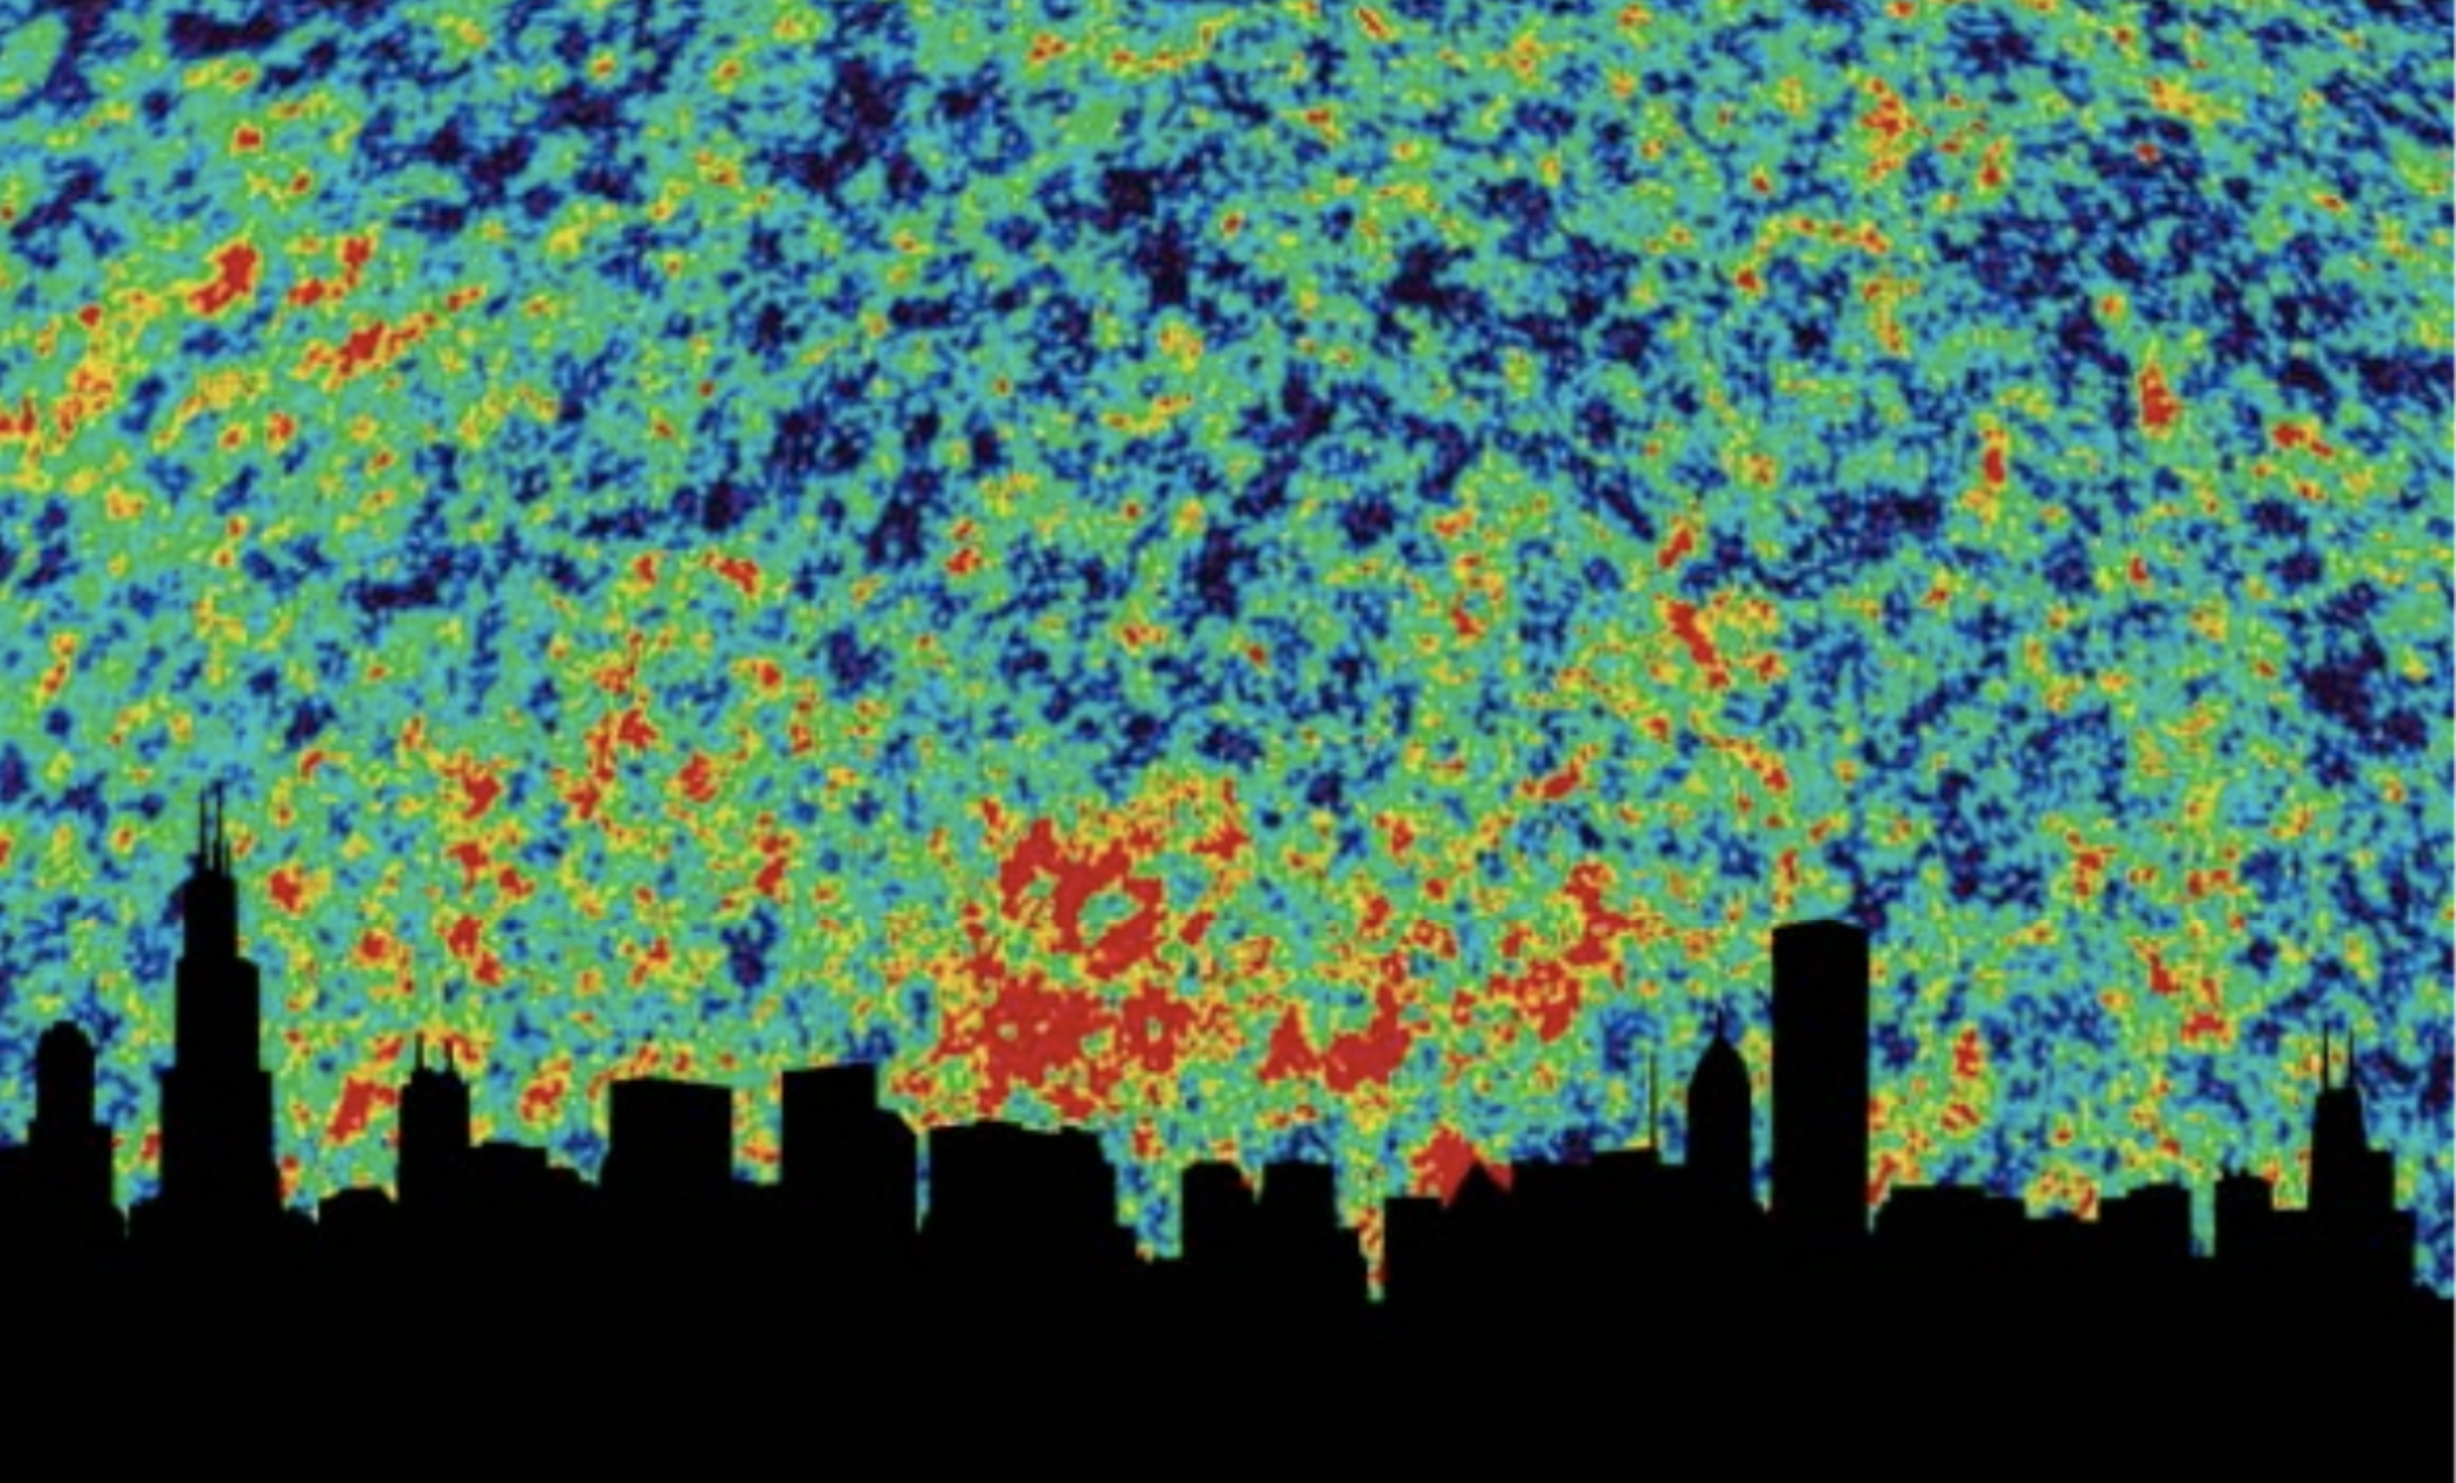
\includegraphics[width=0.4\textwidth]{motivacion1}}
												\only<2>{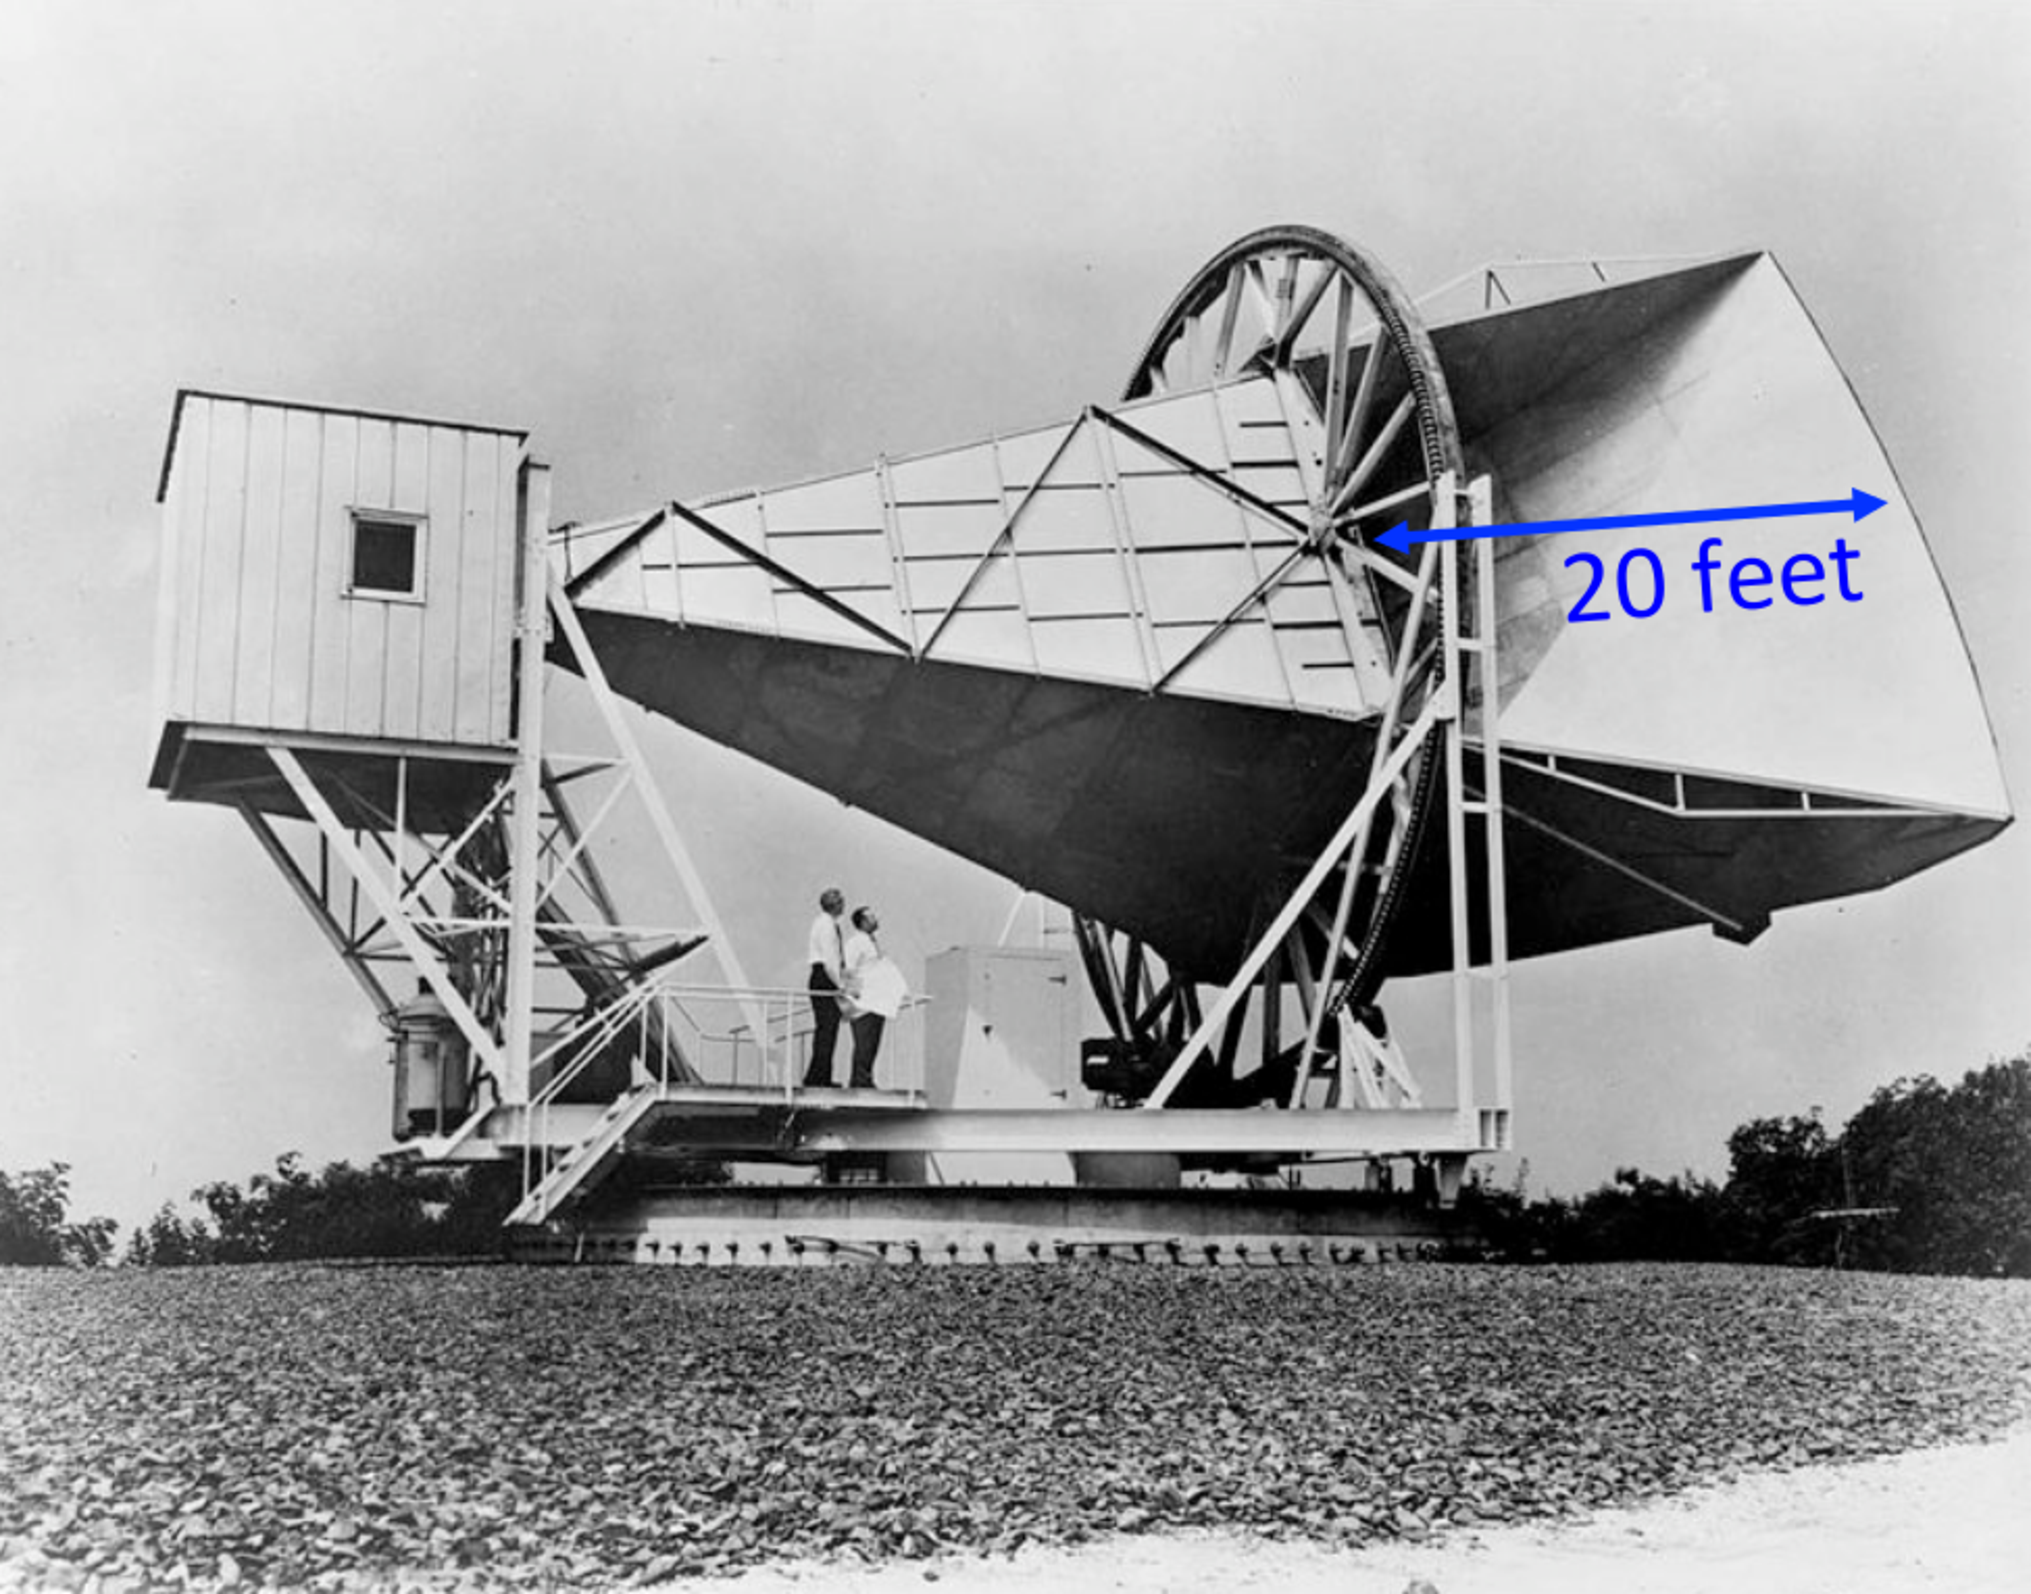
\includegraphics[width=0.4\textwidth]{motivacion2}}
												\only<2>{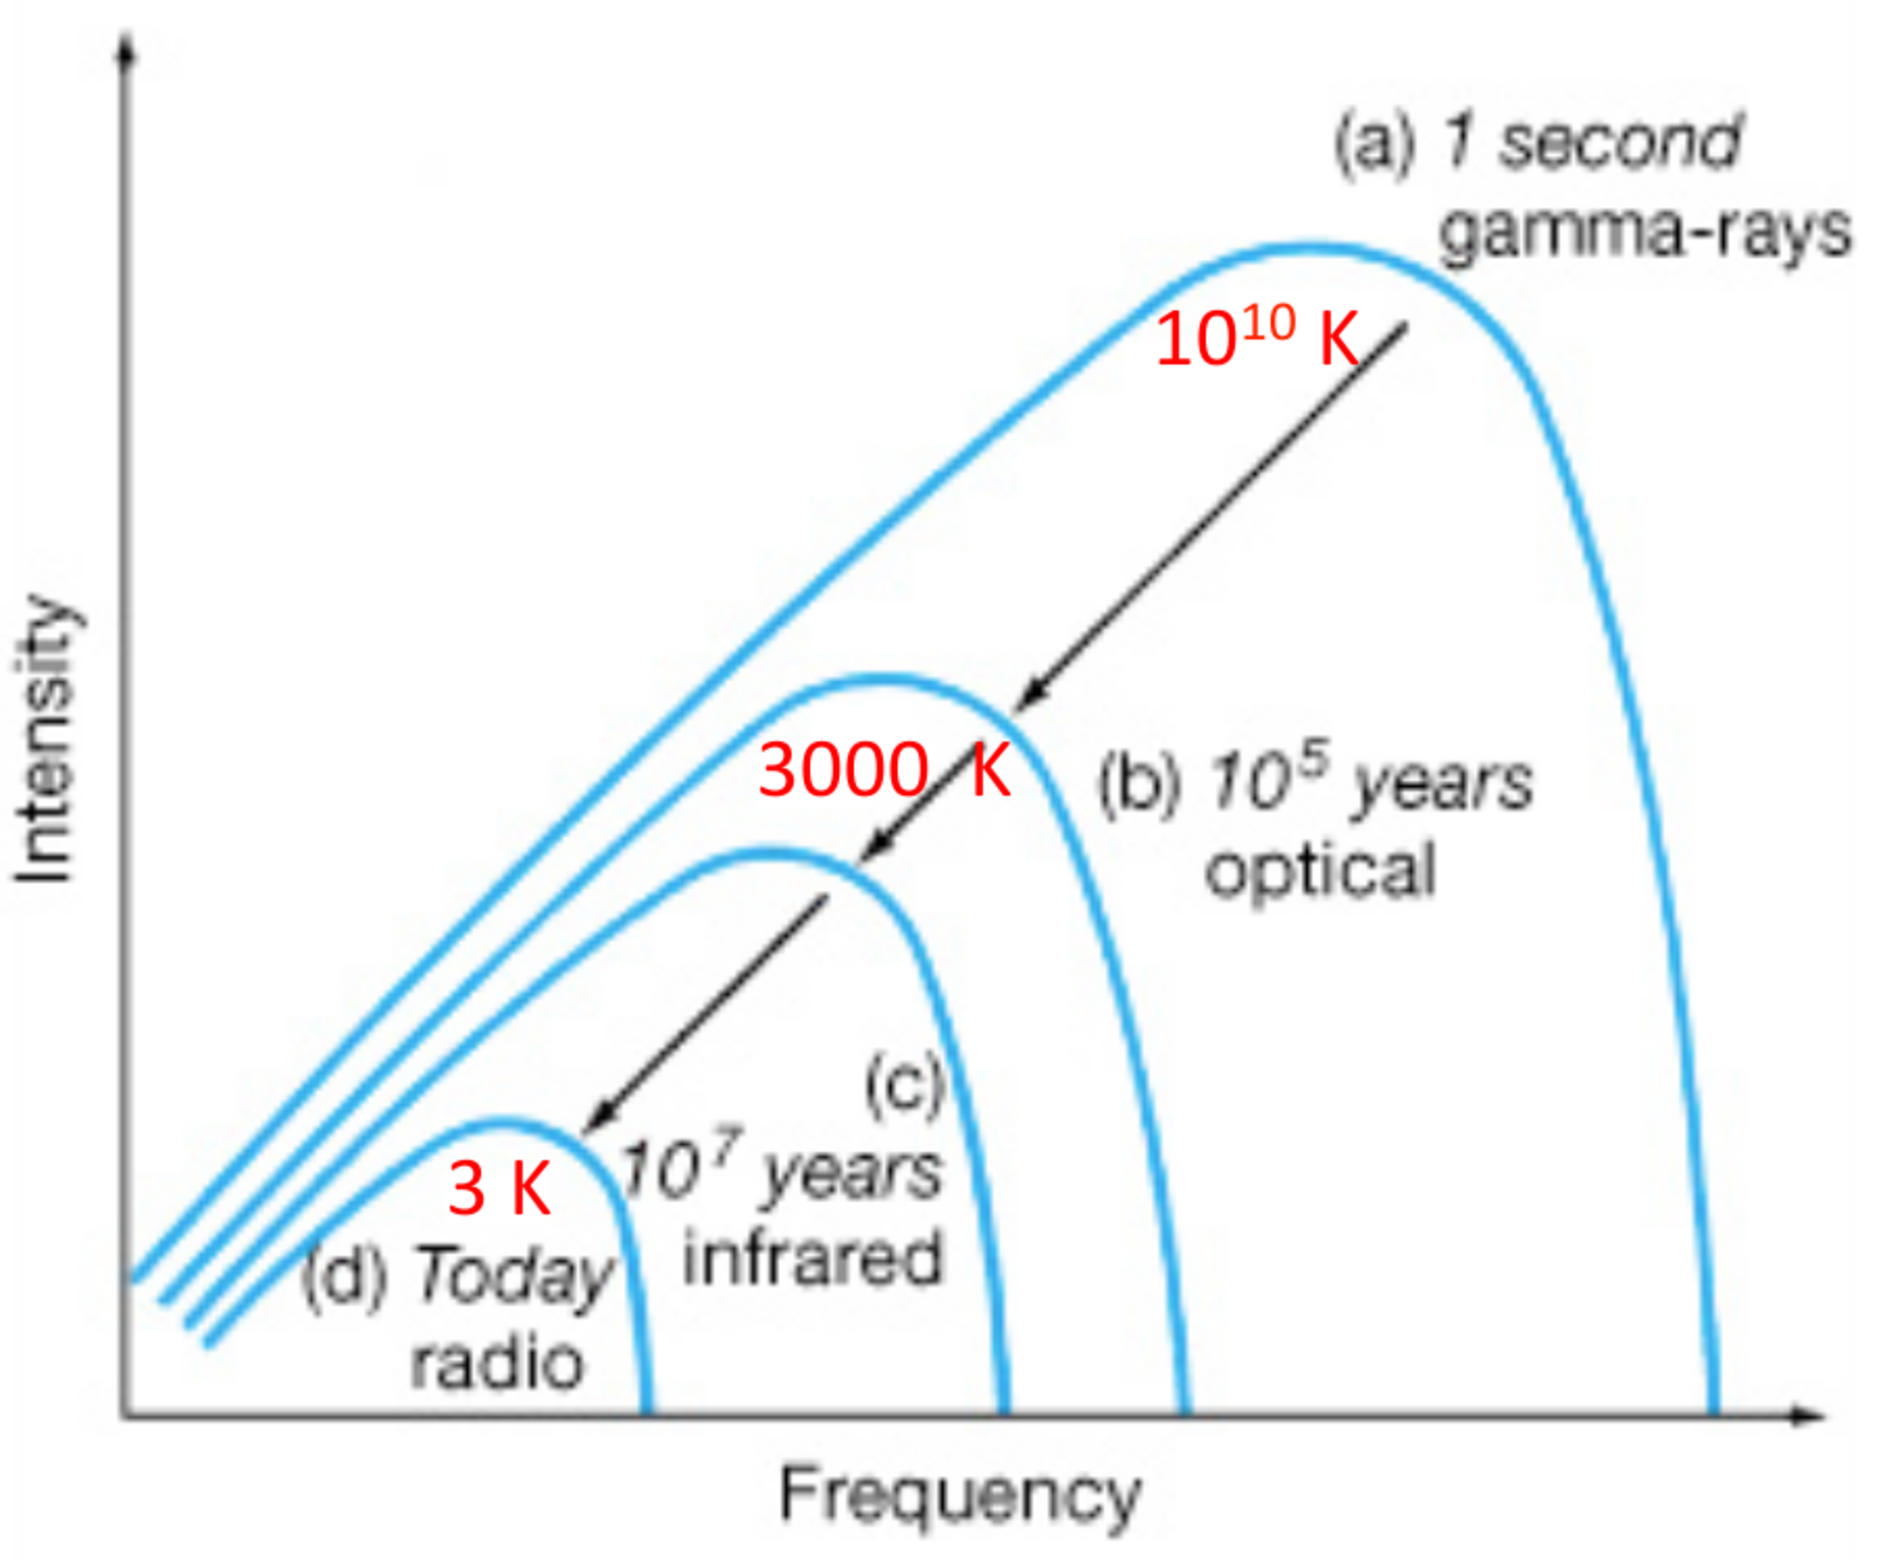
\includegraphics[width=0.4\textwidth]{motivacion3}}
												\only<3>{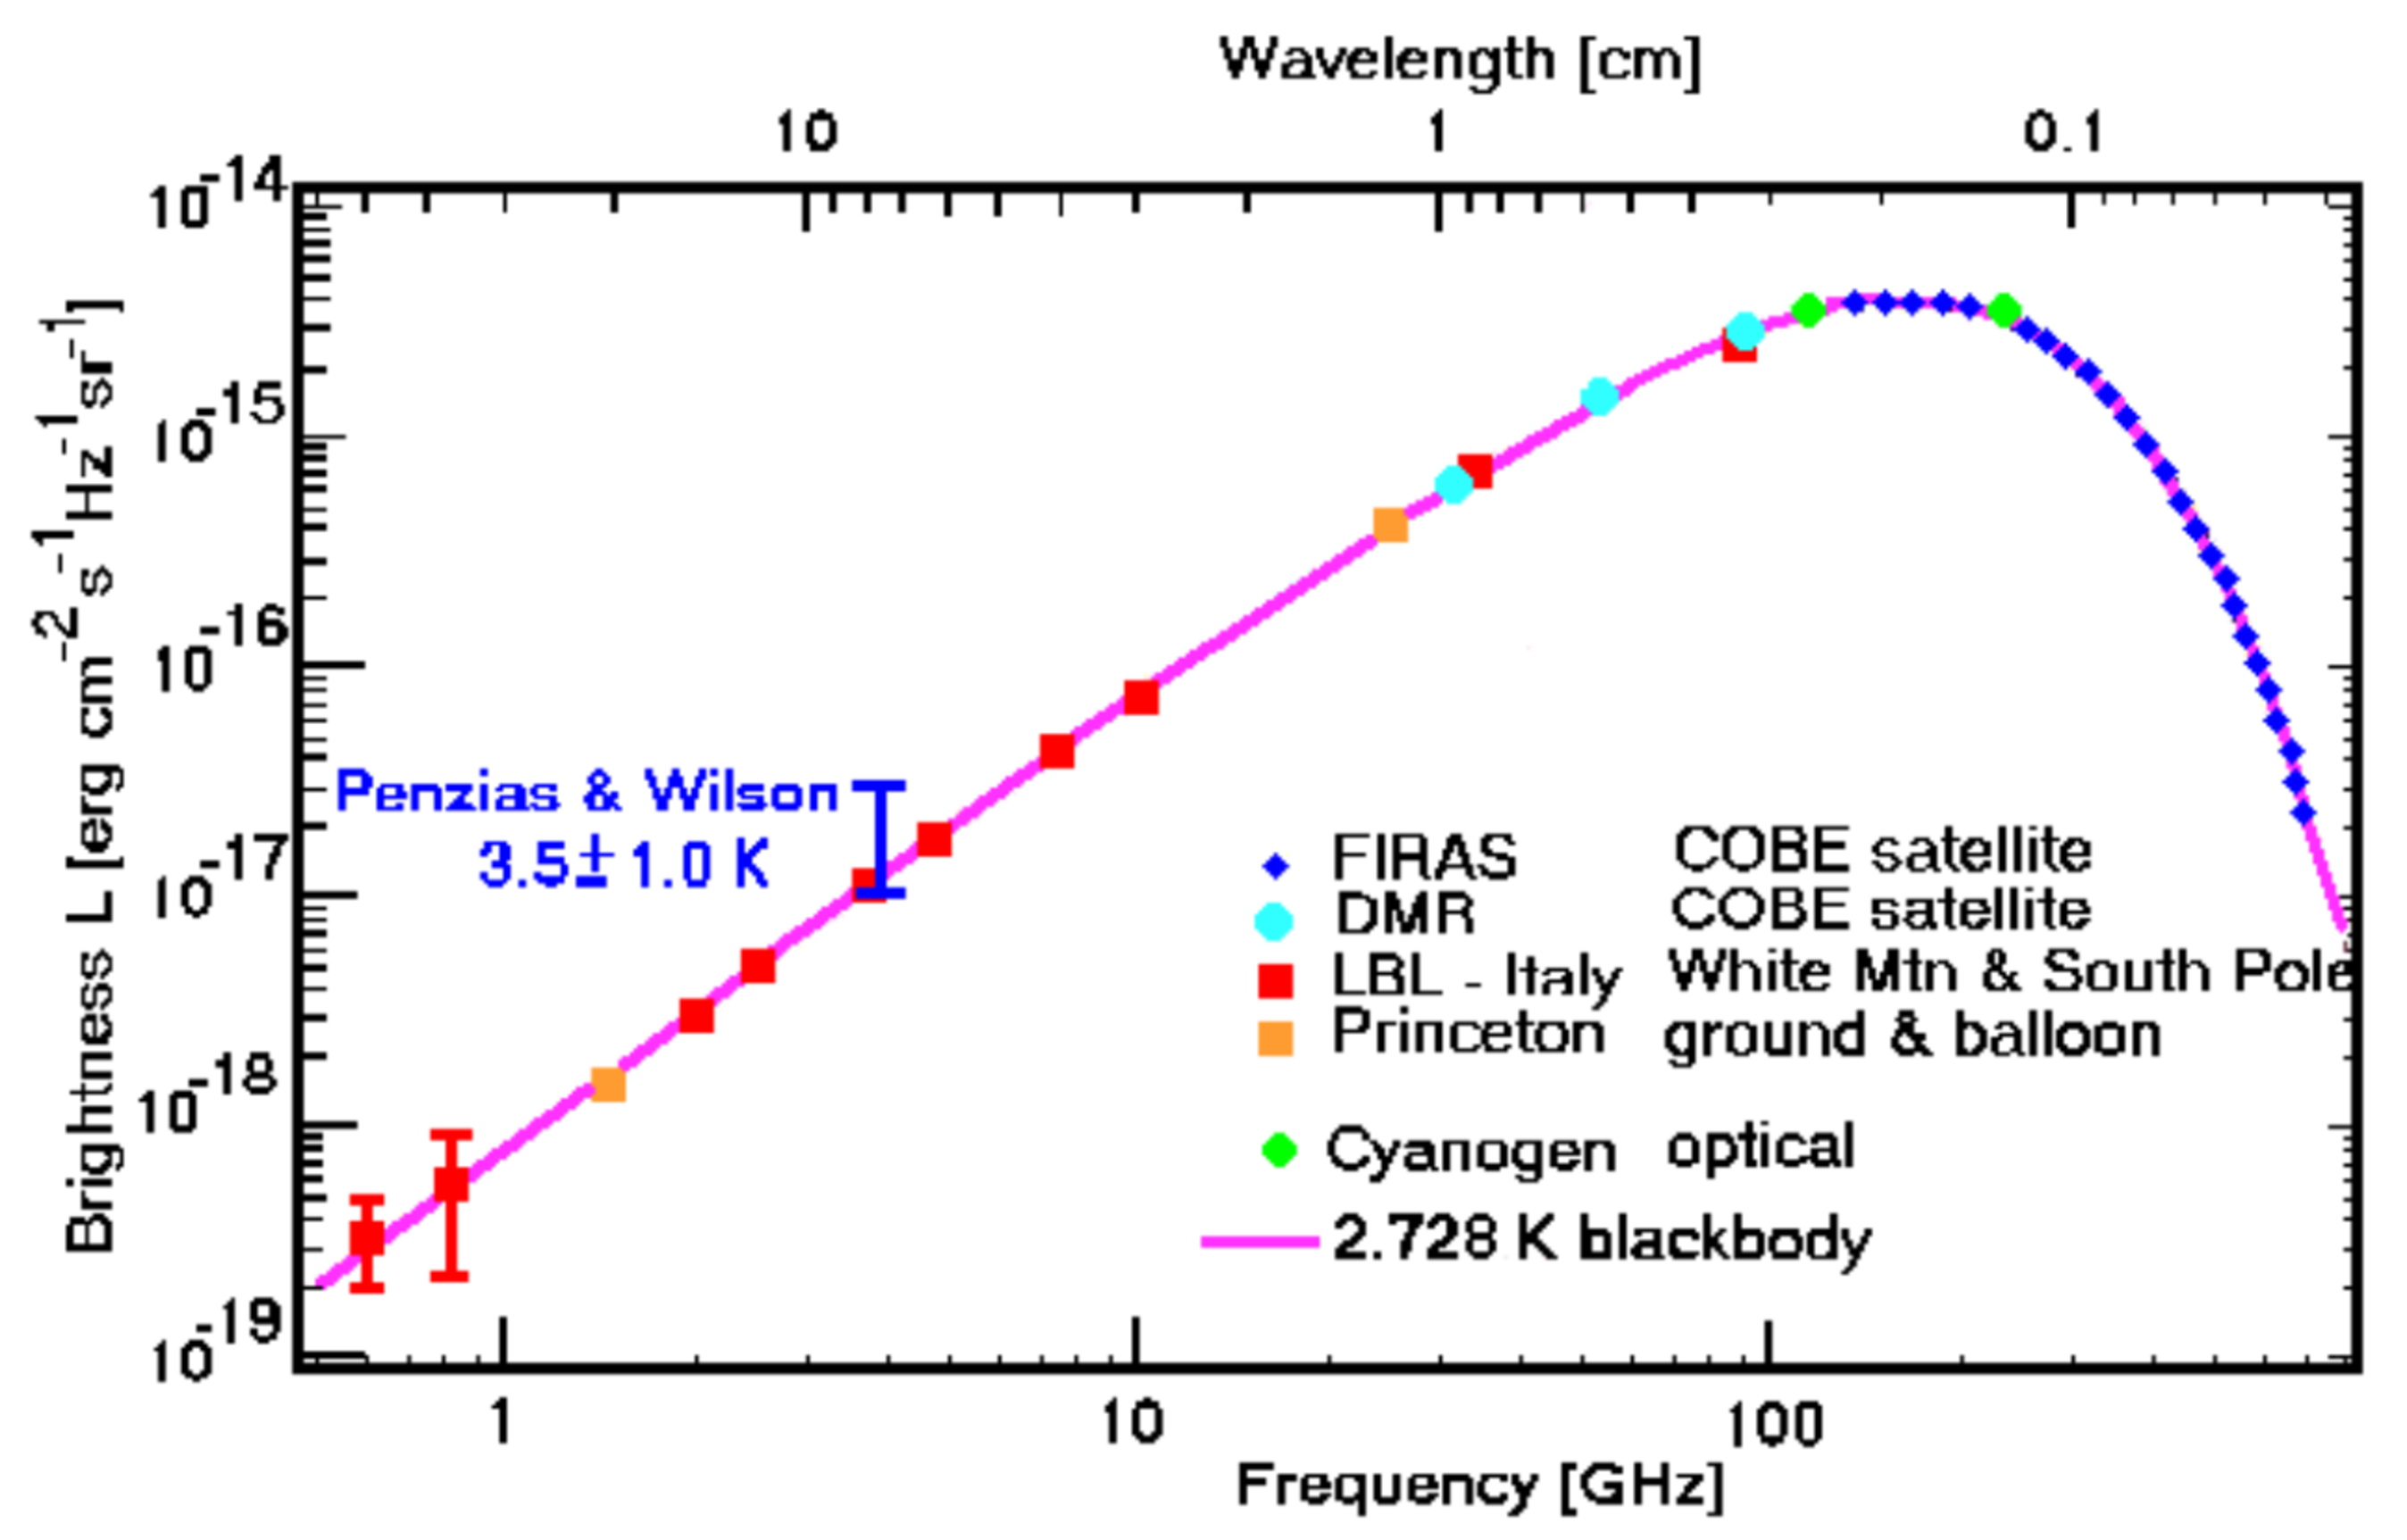
\includegraphics[width=0.6\textwidth]{motivacion4}}
				\begin{itemize}
								\item[*] El fondo cósmico de microondas (CMB) es radiación EM
												de una etapa temprana del universo (Big Bang)
								\item[*] Penzias y Wilson (1964). TELSTAR (1962) 
								\item[*] Expansión del Universo $\to$ temperatura baja
								\only<3>{\item[*] Sus datos (y muchos otros desde entonces) se ajustan a
												la curva teórica para un cuerpo negro de 2.728 K}
				\end{itemize}

\end{frame}
\begin{frame}{Motivación}
				\framesubtitle{Estudios del CMB}
				\begin{columns}
								\begin{column}{0.49\textwidth}
				\begin{itemize}
								\item[*] El hecho de que el CMB tenga un espectro de cuerpo
												negro tan preciso es evidencia de que vino de cuando era
												mucho más caliente y denso de lo que es ahora
								\item[*] Por lo tanto, el espectro del CMB es una fuerte
												evidencia de que el Universo experimentó una etapa de
												``Big Bang caliente''
				\end{itemize}
								\end{column}
								\begin{column}{0.49\textwidth}
												\only<1>{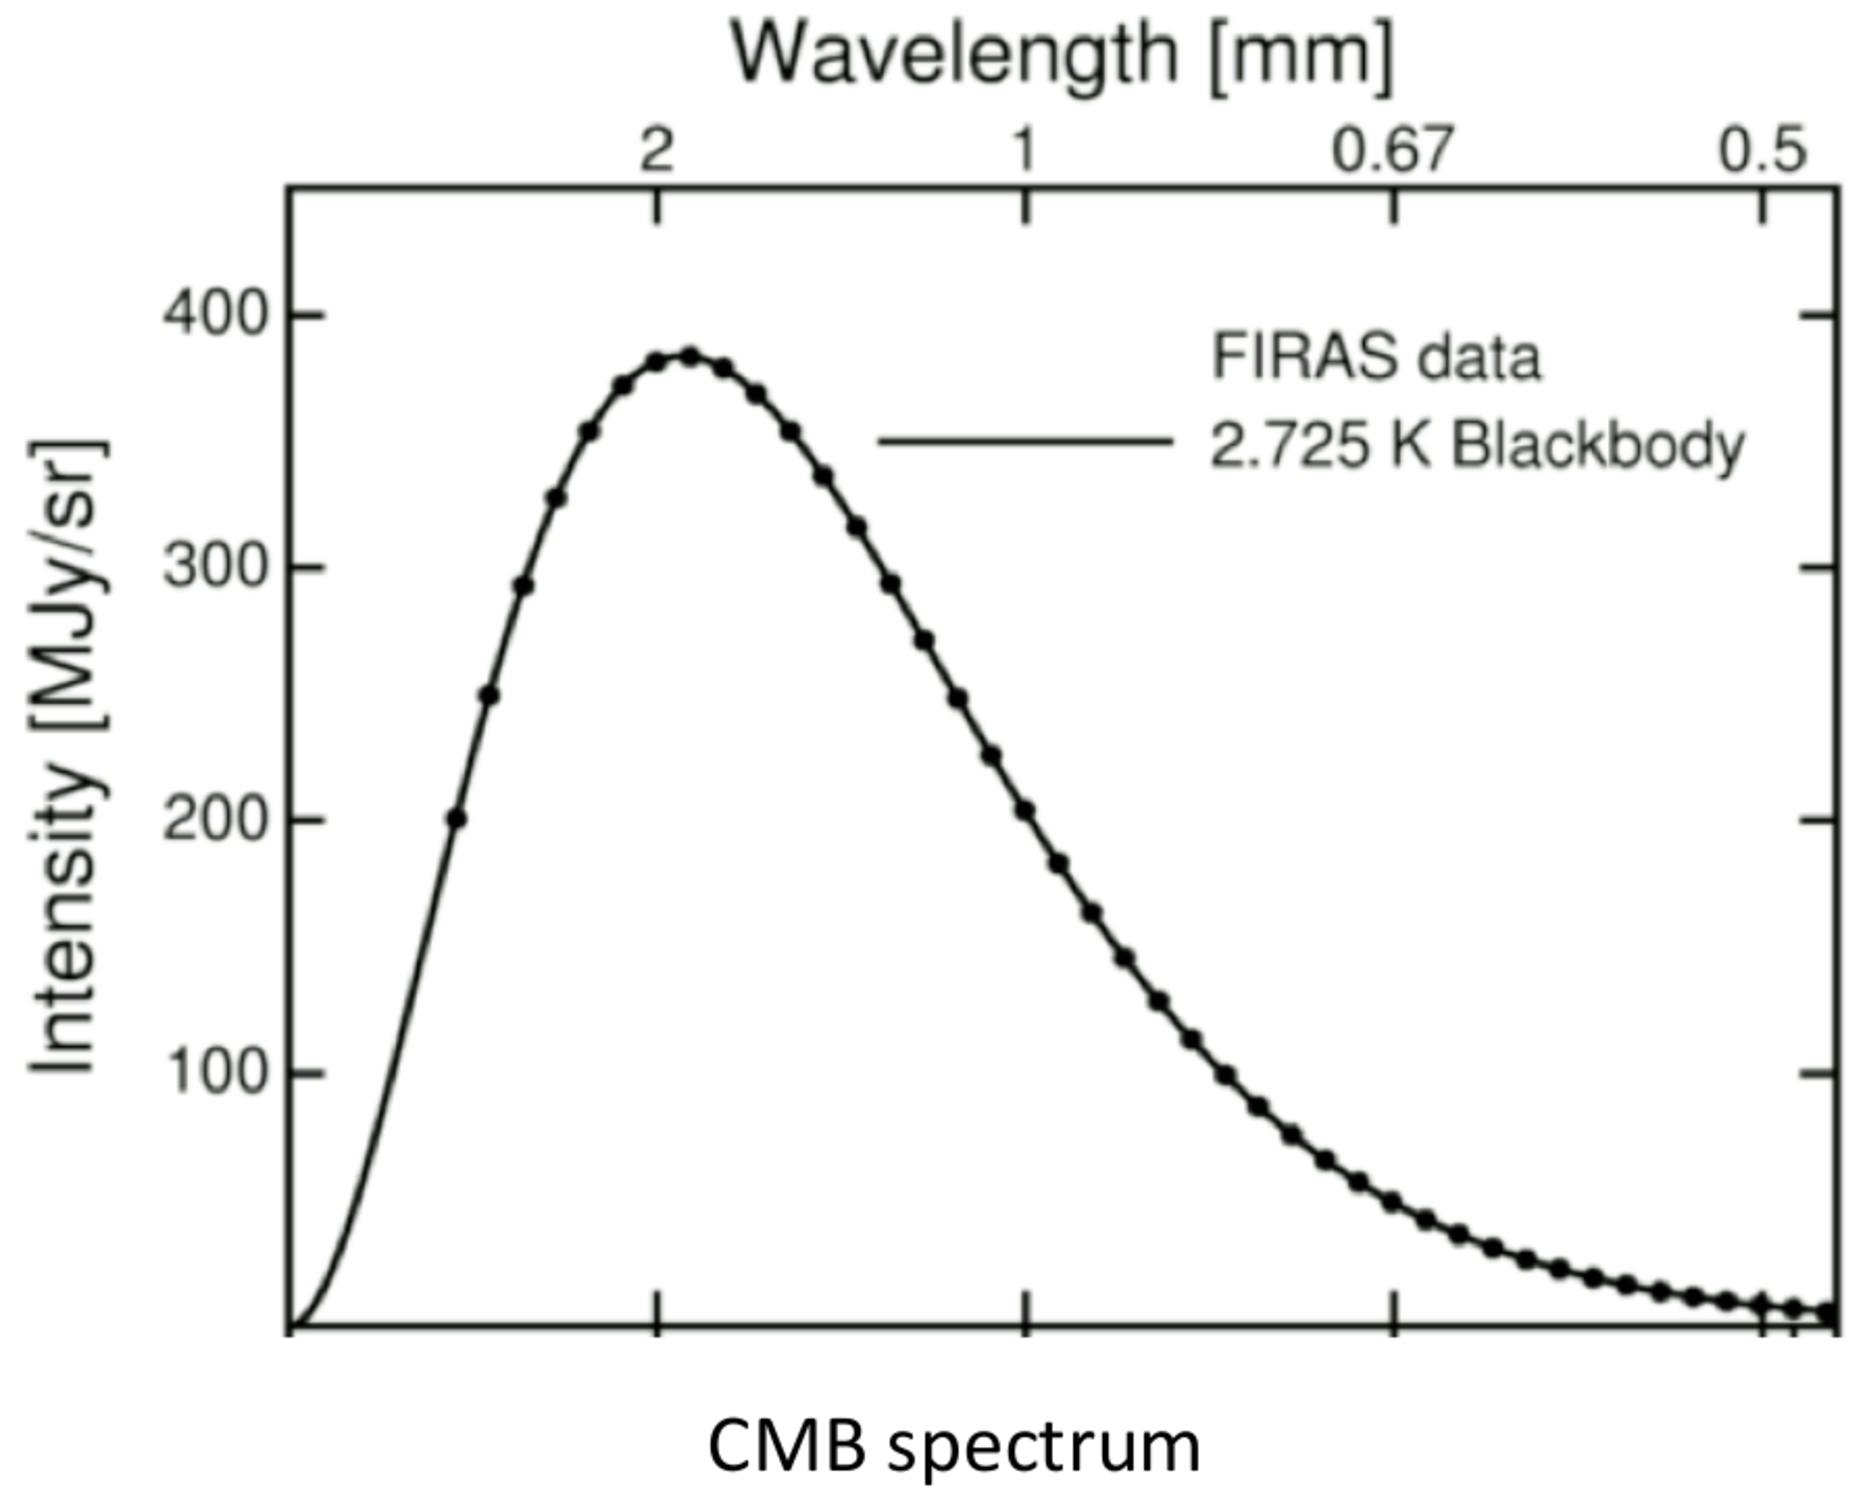
\includegraphics[width=0.9\textwidth]{motivacion5}}
												\only<1>{\includegraphics[width=0.9\textwidth]{c1_cmb_map}}
								\end{column}
								\end{columns}
\end{frame}
\begin{frame}{Motivación}
				\framesubtitle{Estudios del CMB}
				\begin{columns}
								\begin{column}{0.49\textwidth}
				\begin{itemize}
								\item[*] Anisotropías: Los colores indican variaciones de
												temperatura: rojo para más caliente, azul para más
												frío
								\item[*] Tamaños de los puntos calientes y fríos $\to$
												cálculos de valores fundamentales para la forma, tamaño,
												edad, contenido, tasa de expansión (y más) de nuestro
												universo
				\end{itemize}
								\end{column}
								\begin{column}{0.49\textwidth}
												\only<1>{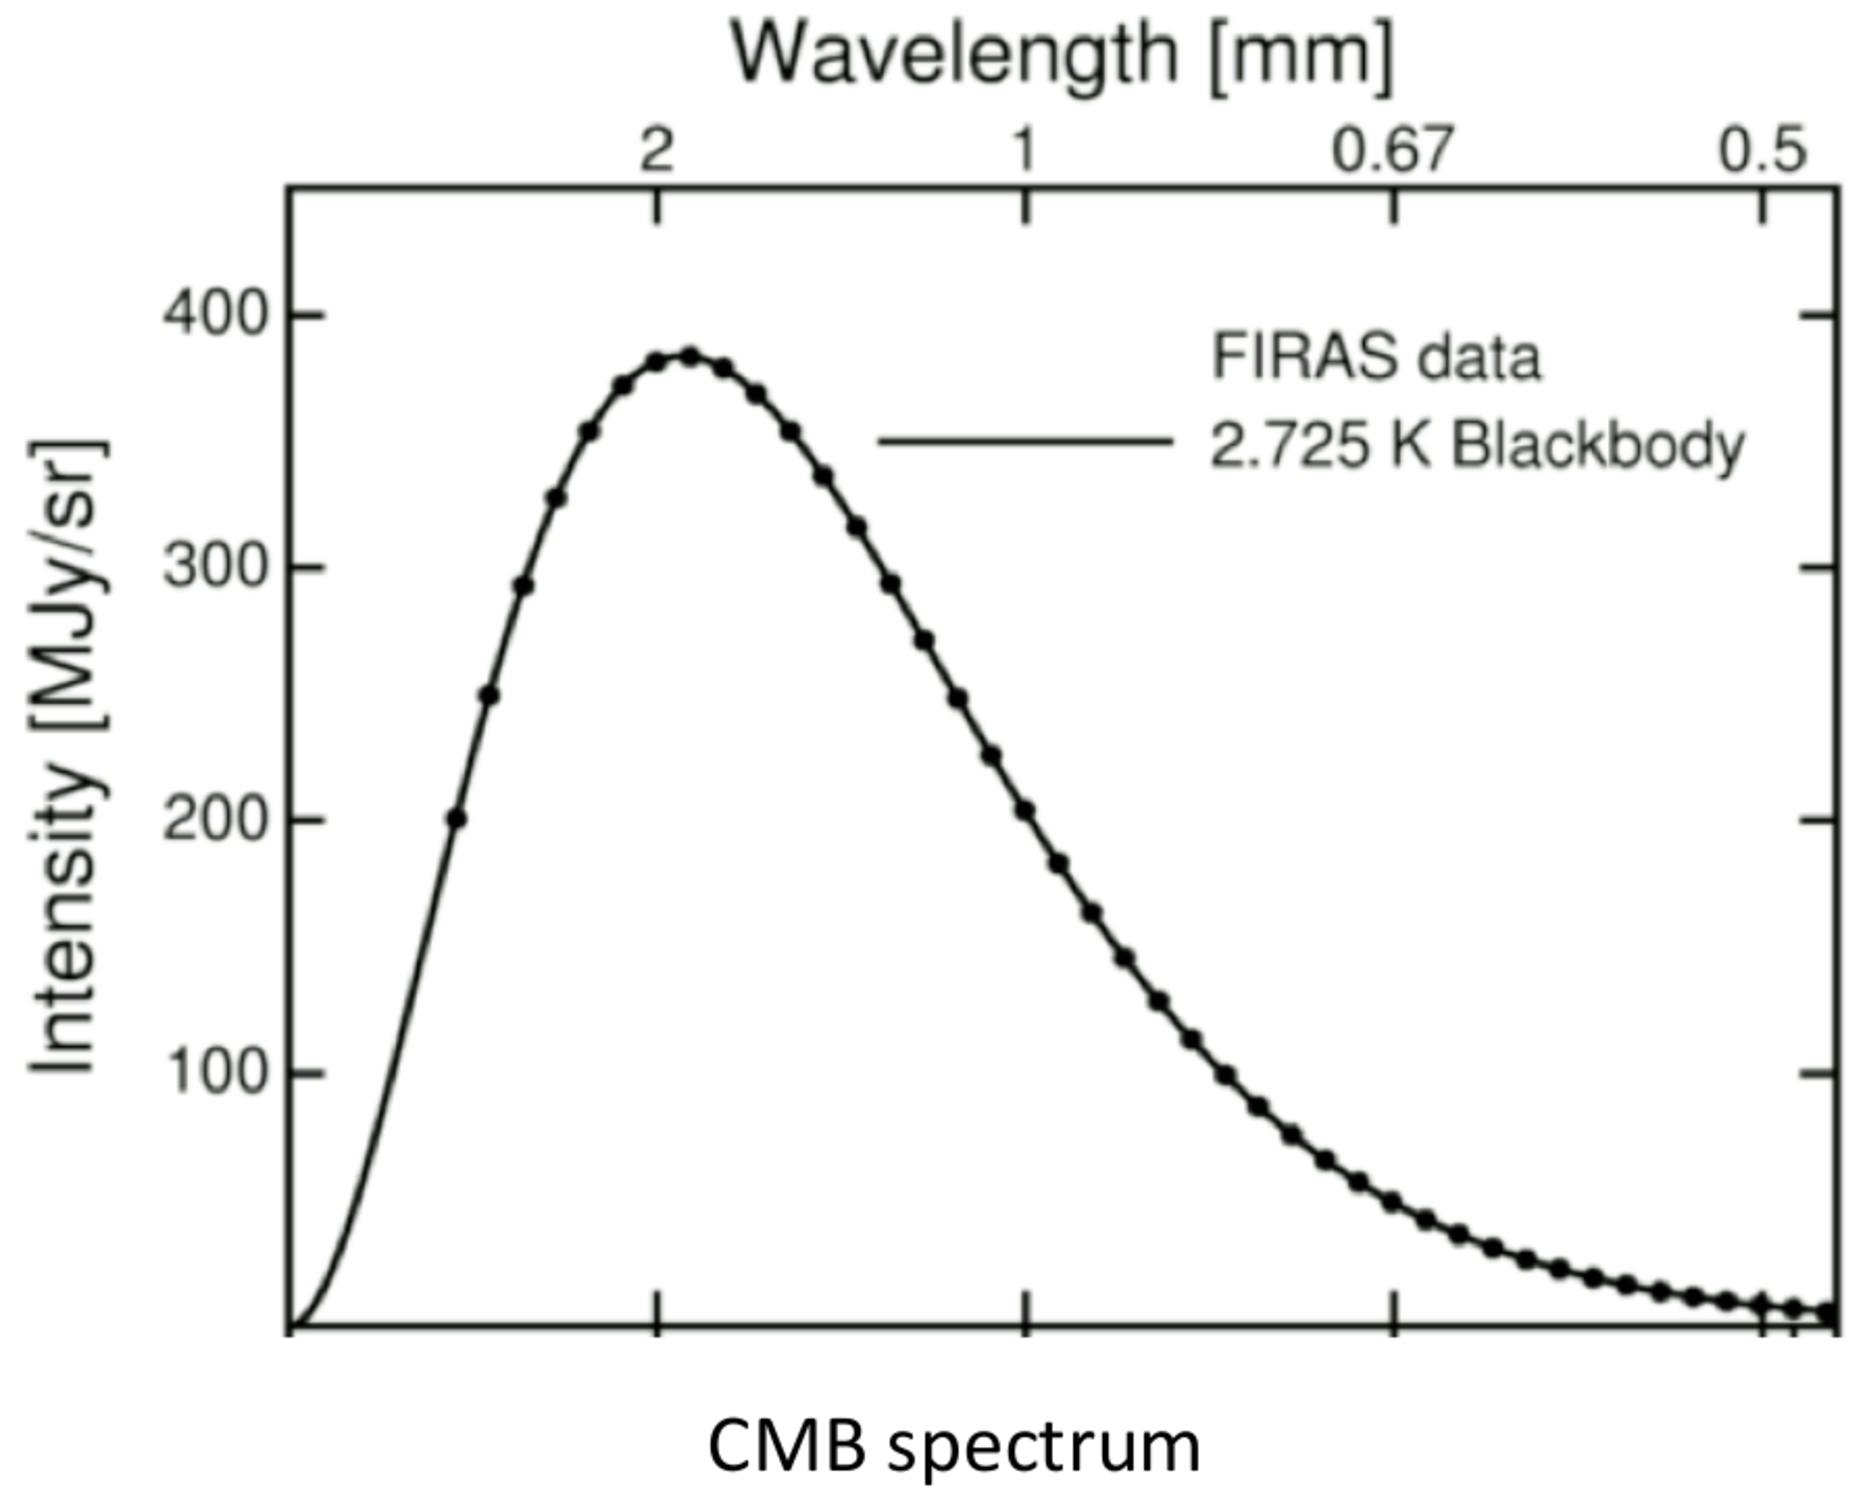
\includegraphics[width=0.9\textwidth]{motivacion5}}
												\only<1>{\includegraphics[width=0.9\textwidth]{c1_cmb_map}}
								\end{column}
								\end{columns}
\end{frame}
\begin{frame}{Motivación}
				\framesubtitle{QUBIC}
												\only<1>{\includegraphics[width=0.4\textwidth]{c1_cmb_map}}
												\only<1>{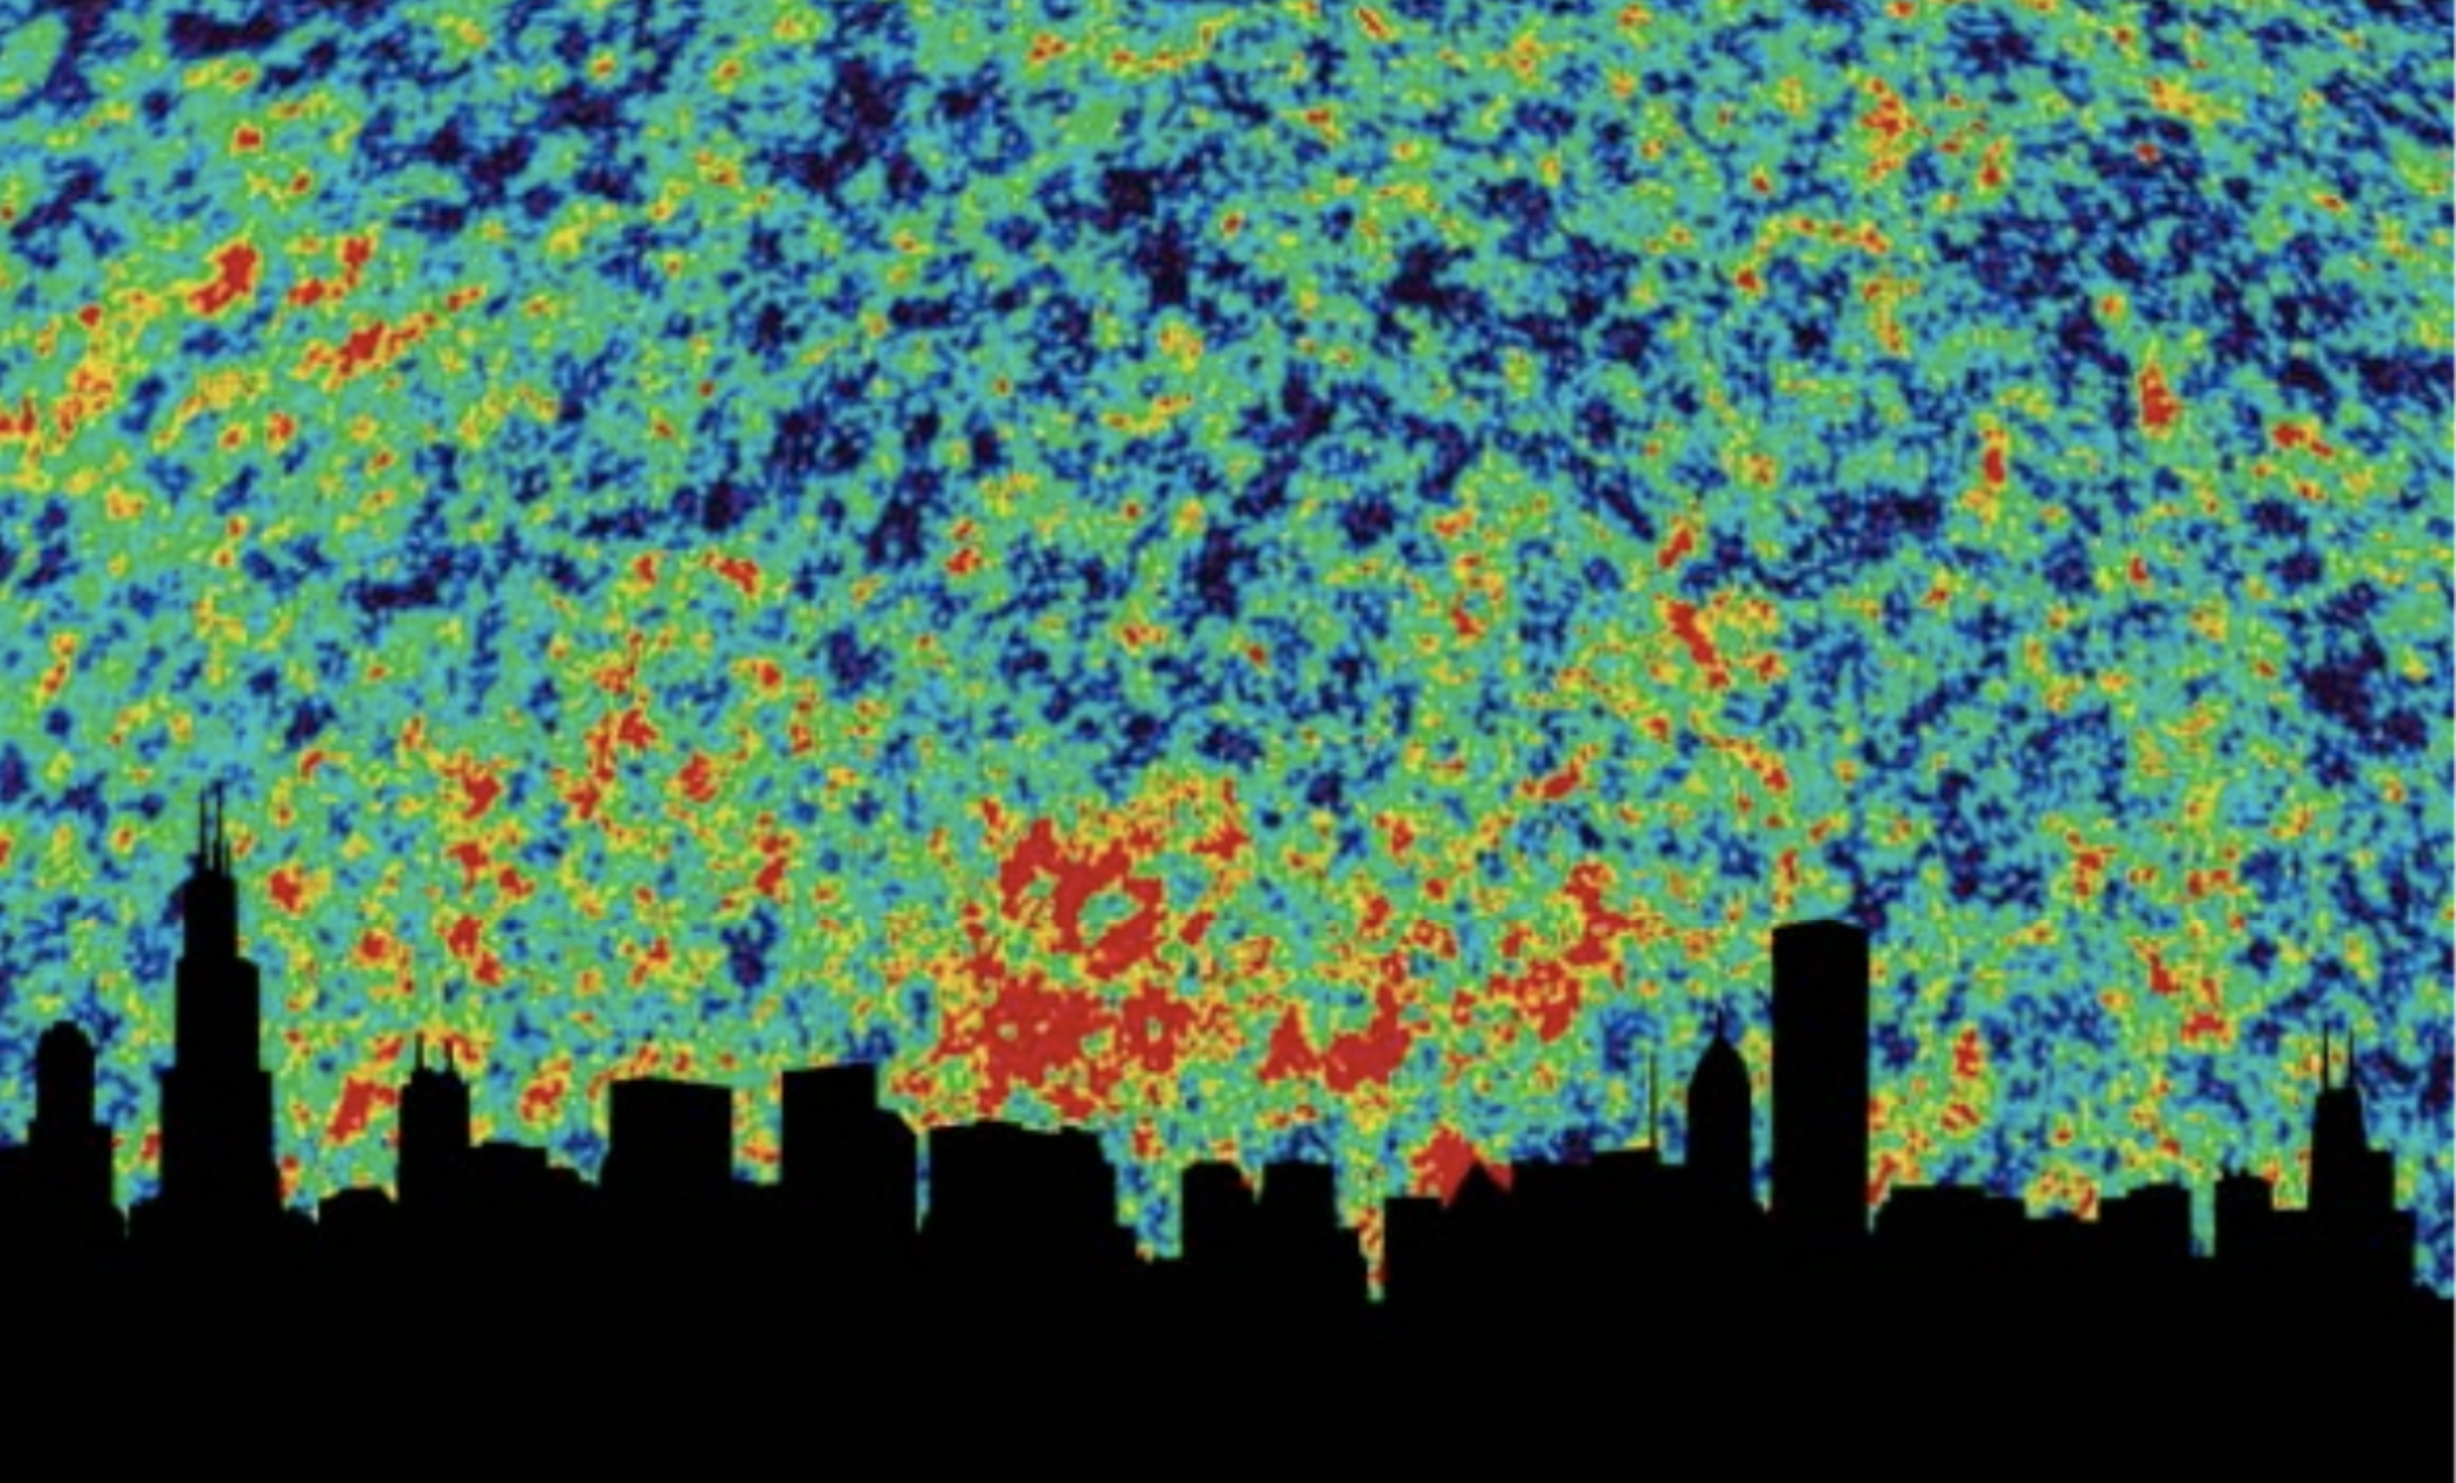
\includegraphics[width=0.4\textwidth]{motivacion1}}
												\only<2>{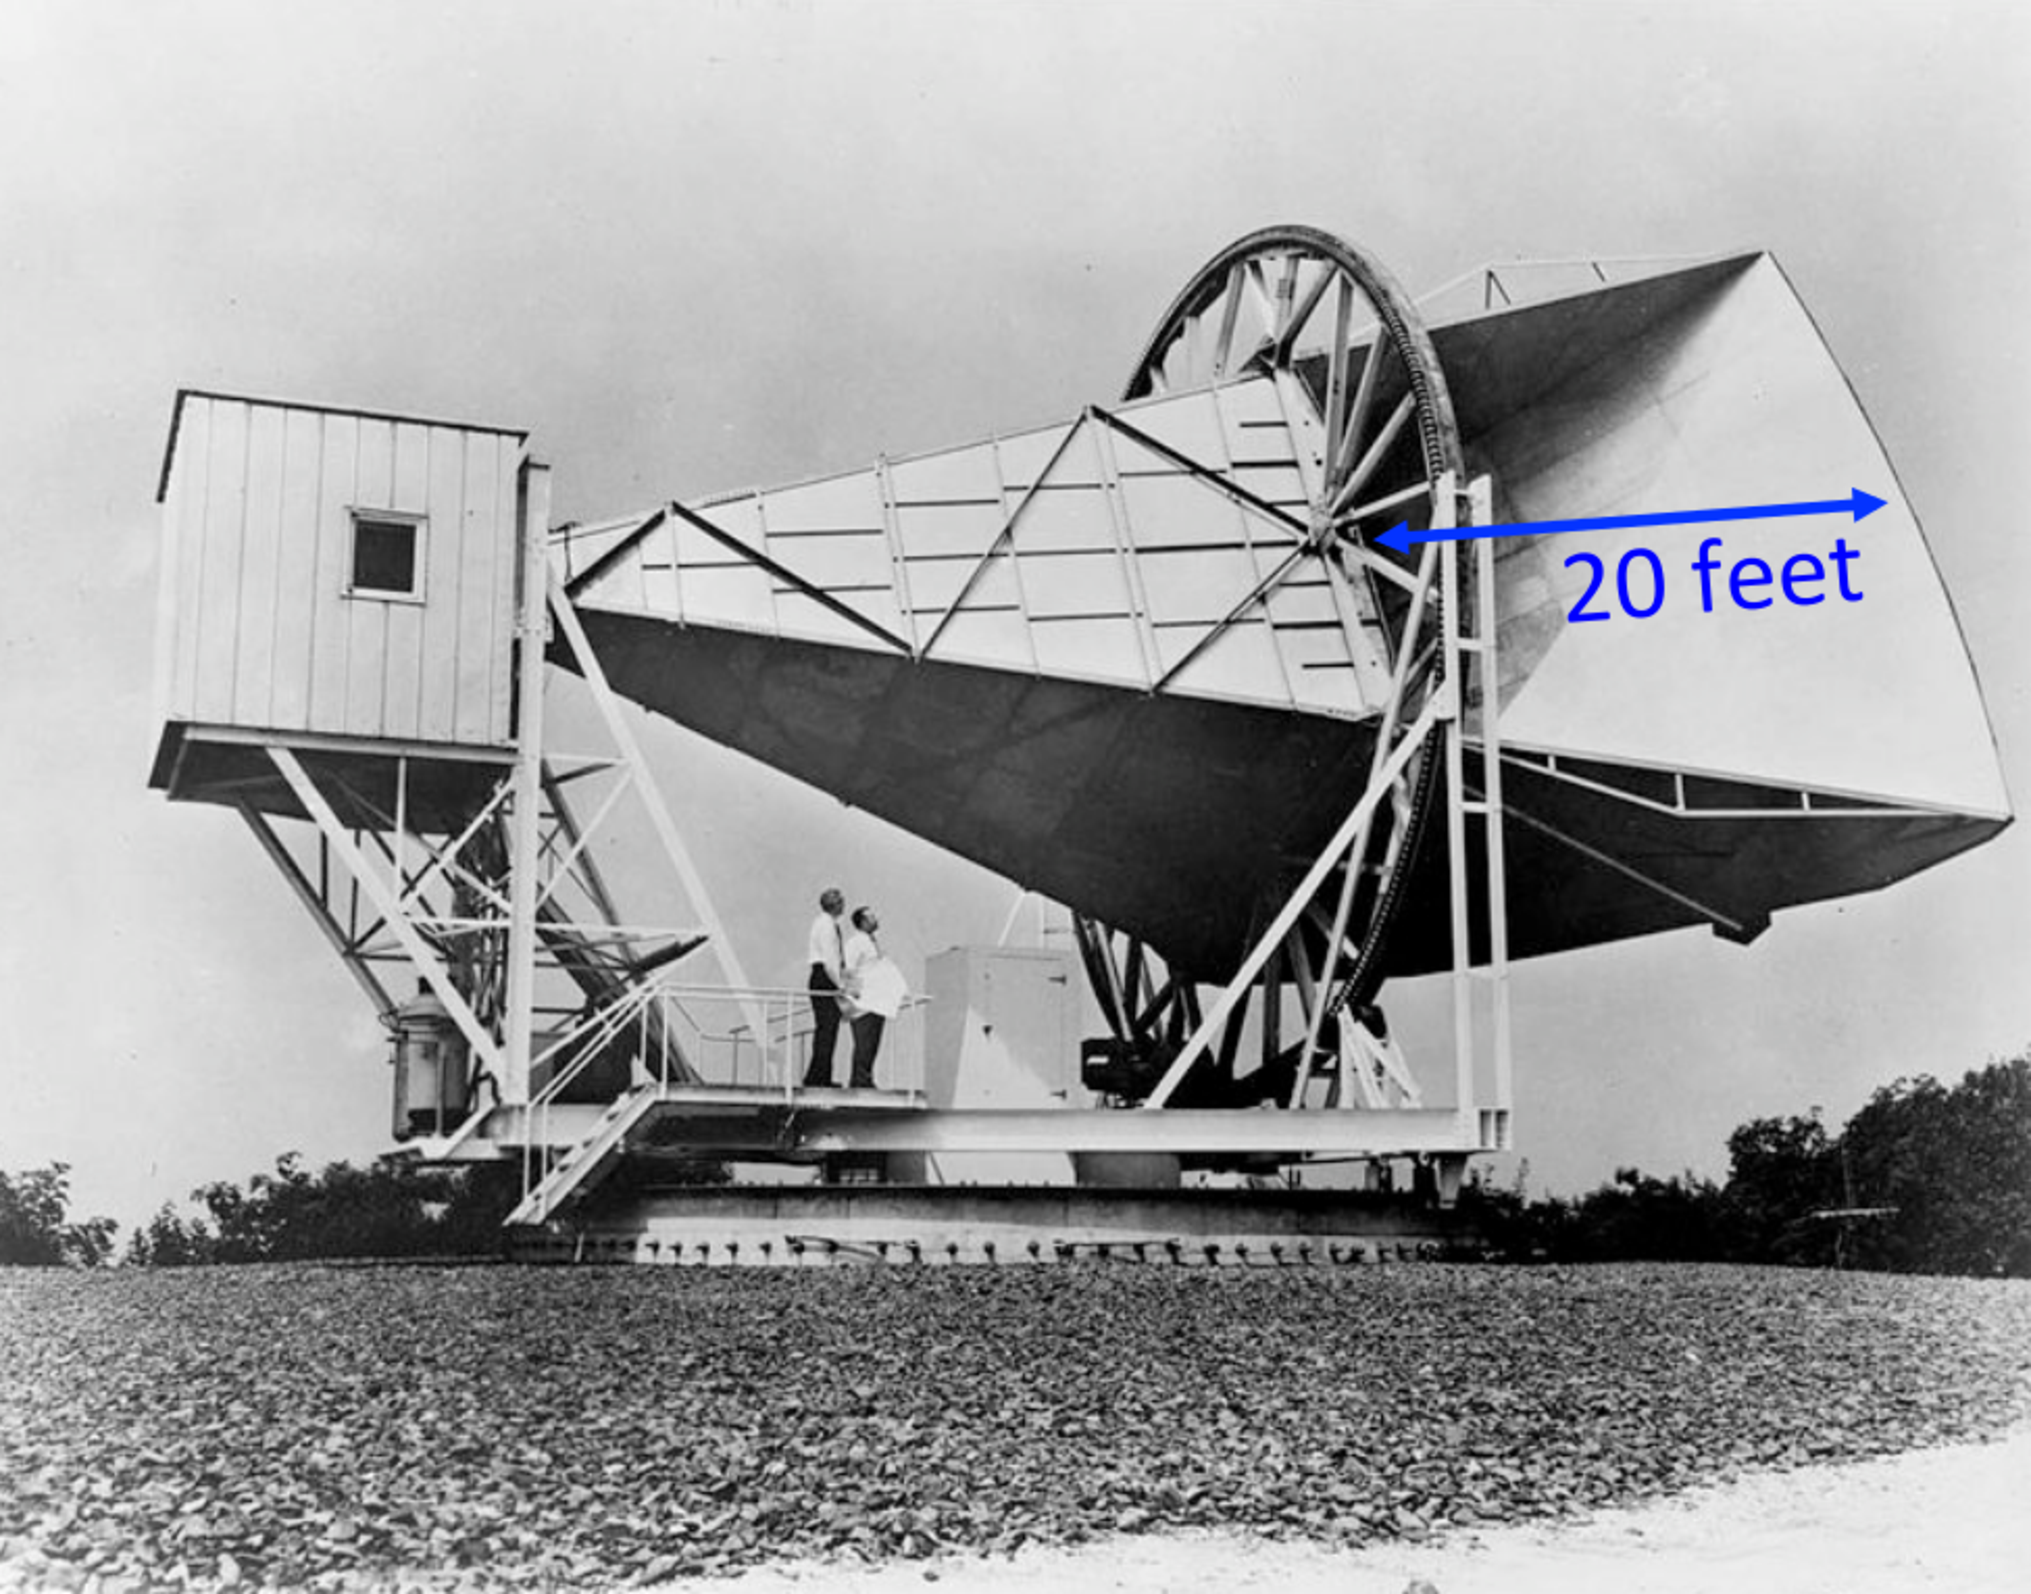
\includegraphics[width=0.4\textwidth]{motivacion2}}
												\only<2>{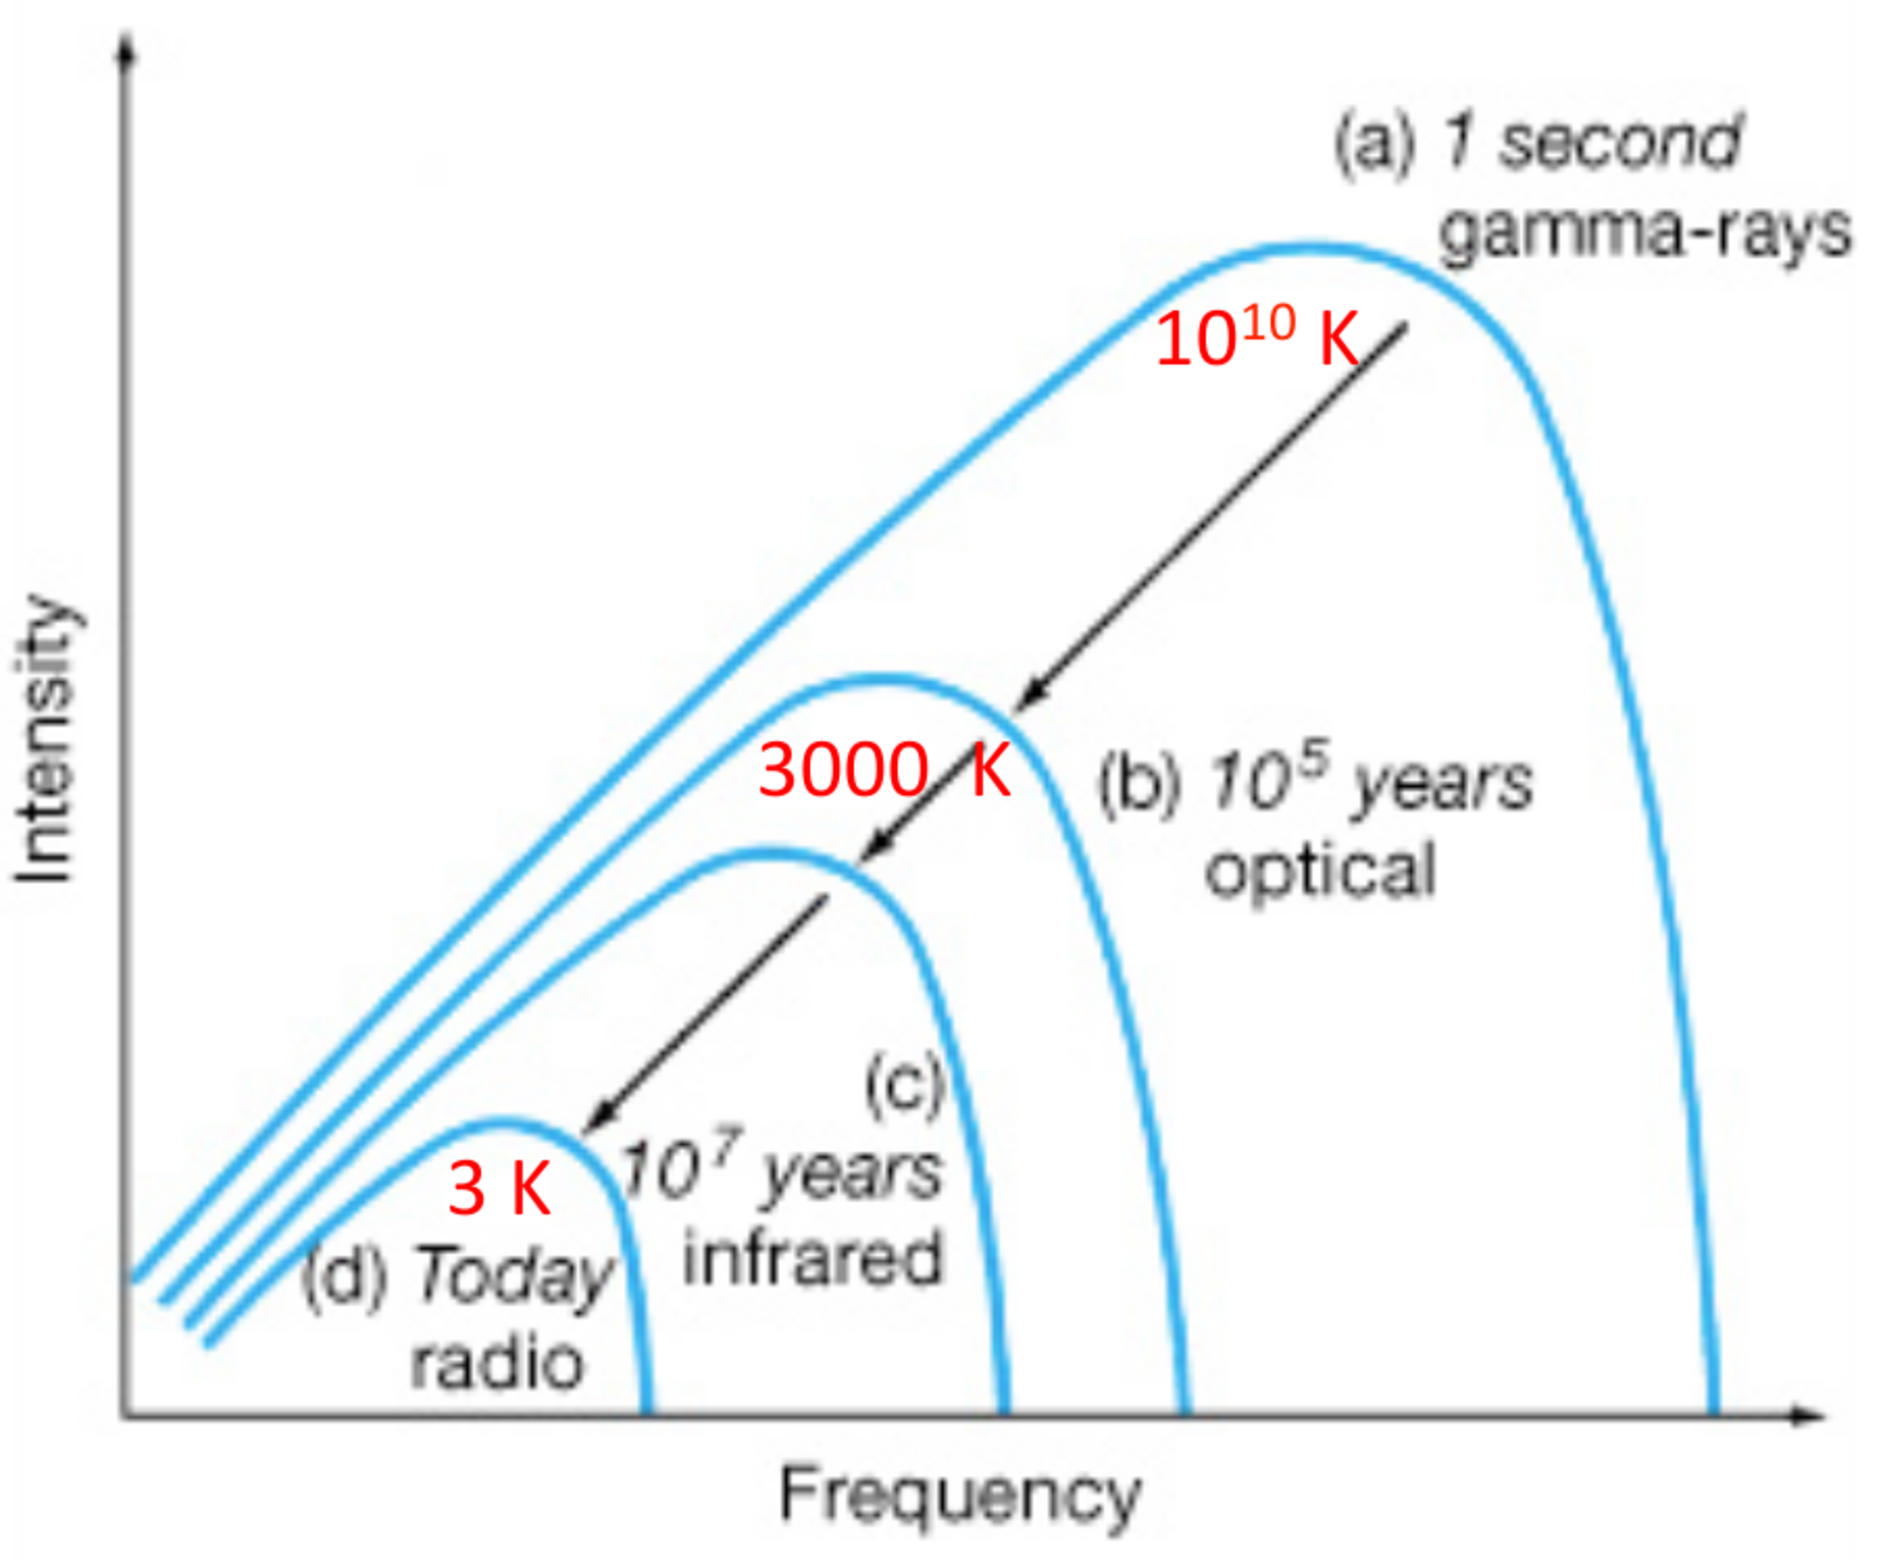
\includegraphics[width=0.4\textwidth]{motivacion3}}
												\only<3>{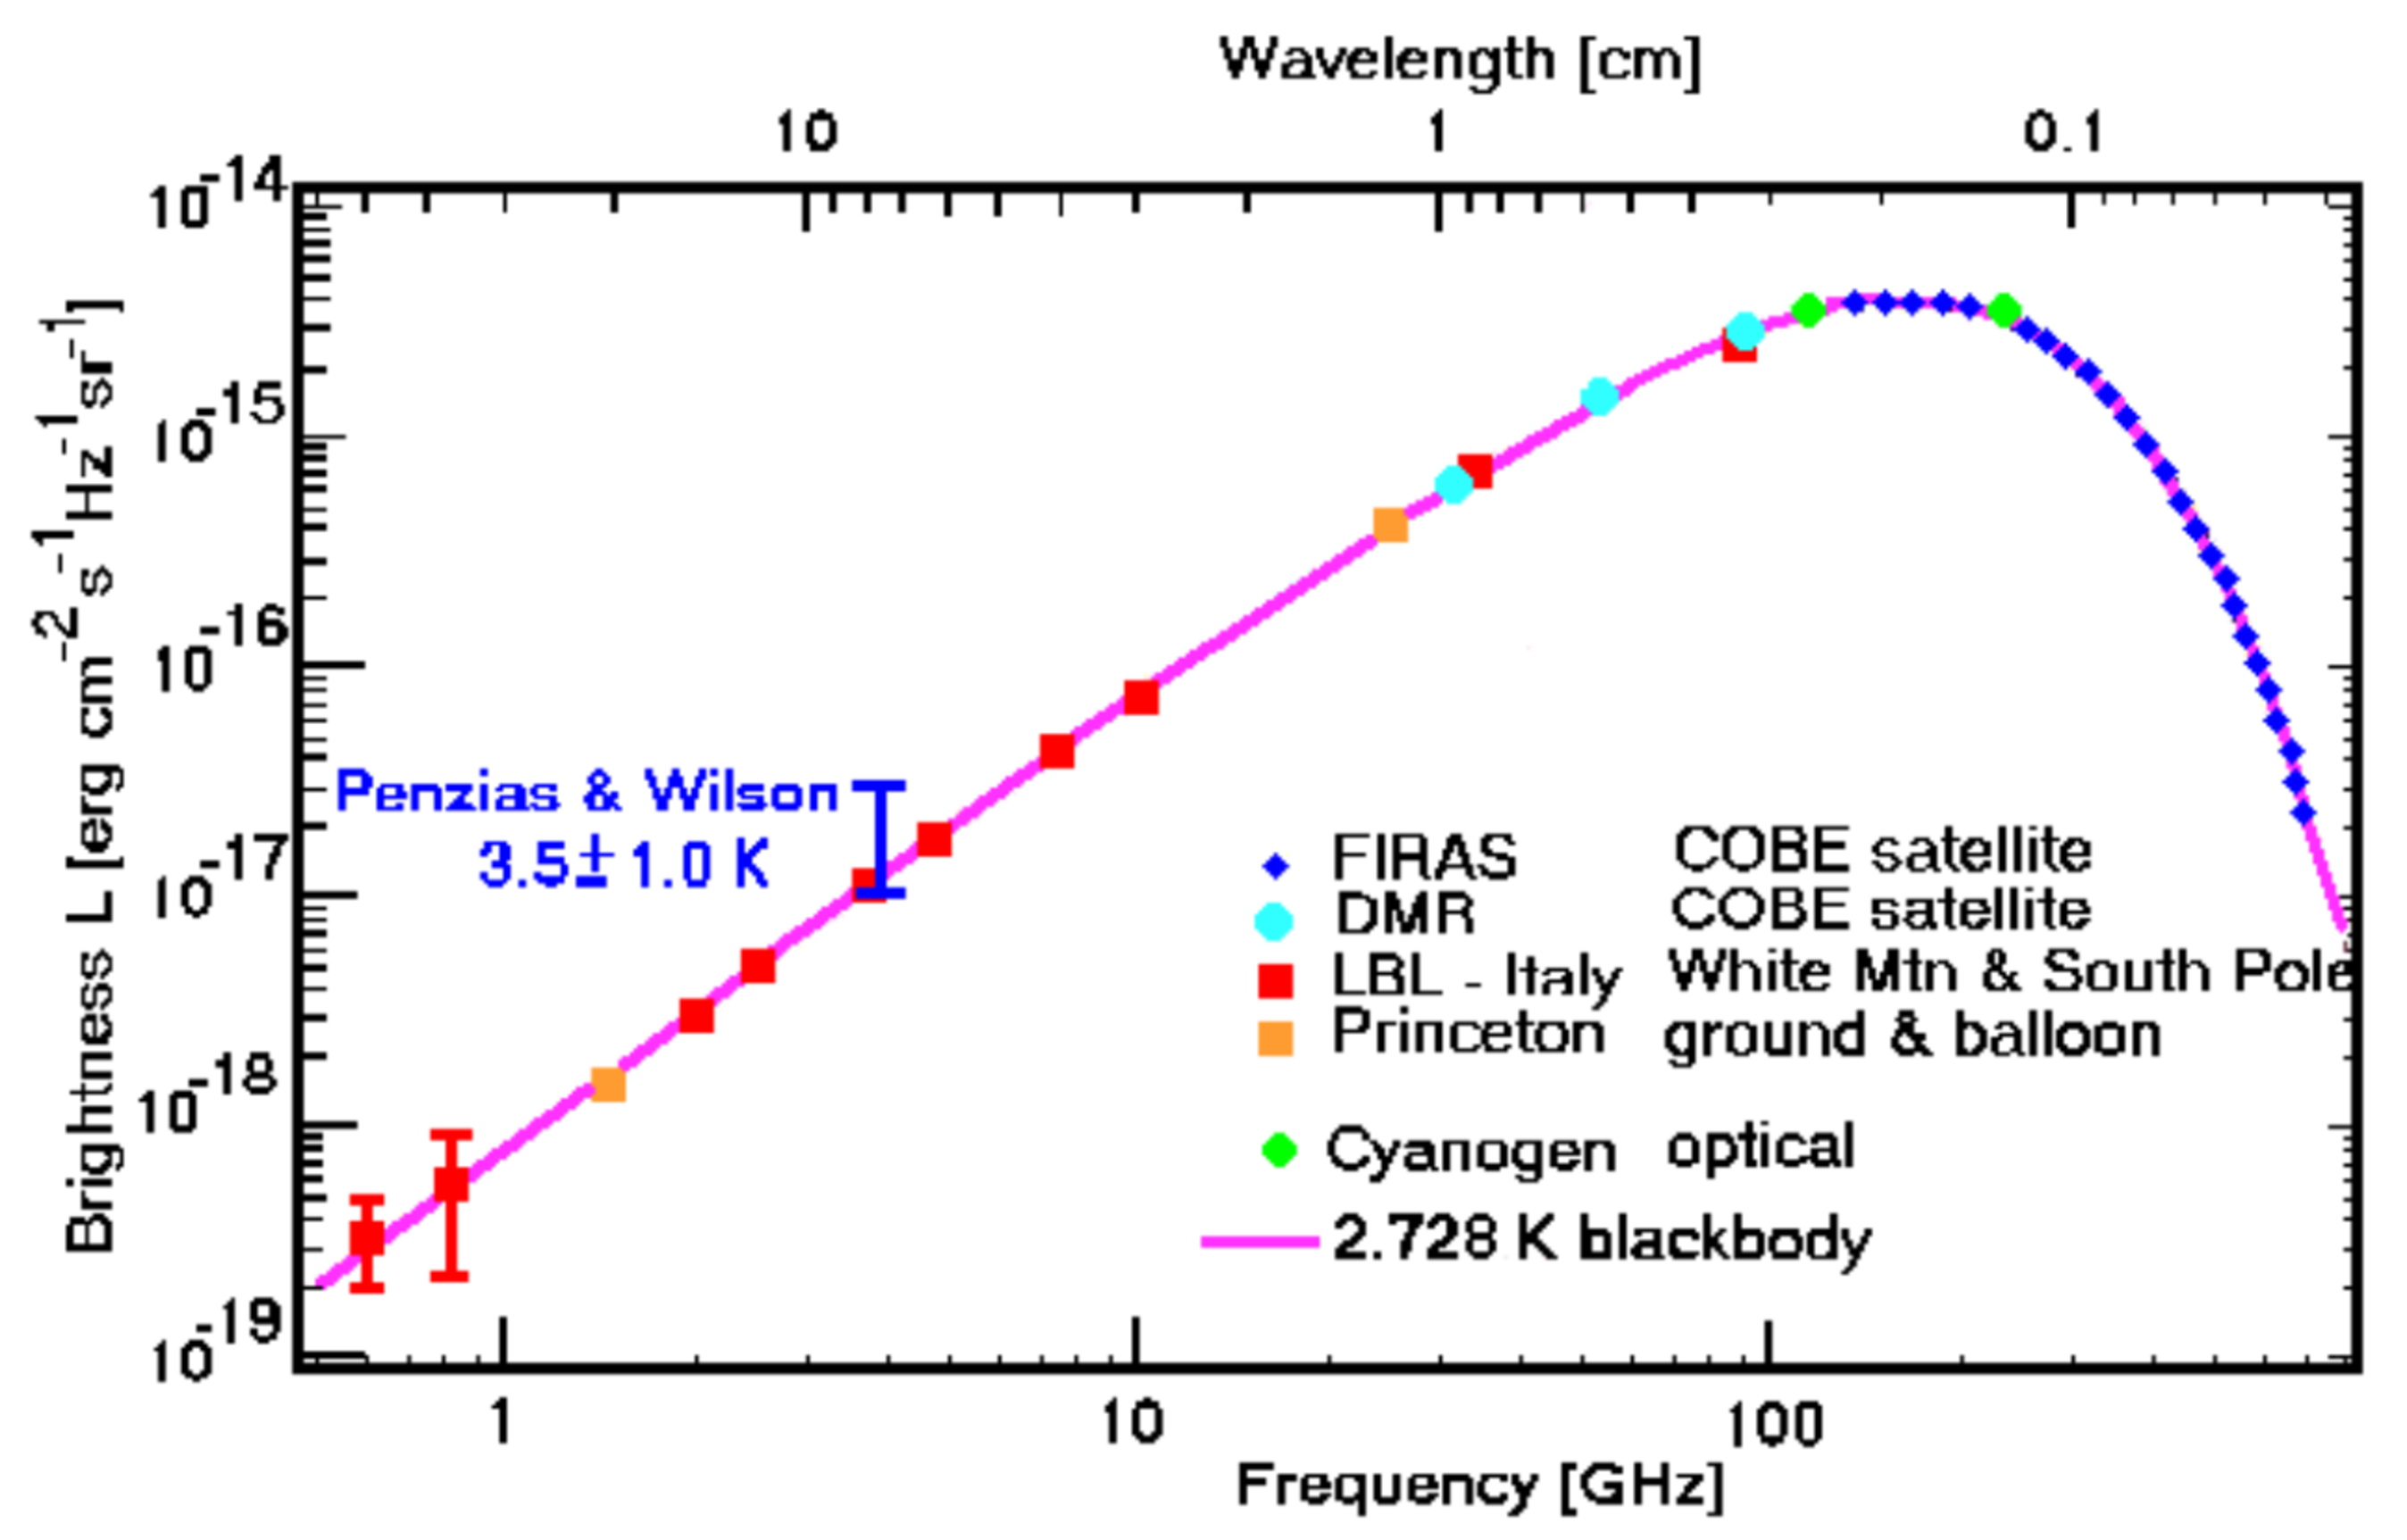
\includegraphics[width=0.6\textwidth]{motivacion4}}
				\begin{itemize}
								\item[*] 
												
								\item[*] 
								\item[*] 
								\only<3>{\item[*] Sus datos (y muchos otros desde entonces) se ajustan a
												la curva teórica para un cuerpo negro de 2.728 K}
				\end{itemize}
\end{frame}

%------------------------------------------------------------------------------
\section{MKIDs}
\begin{frame}{\textbf{M}icrowave \textbf{K}inetic \textbf{I}nductance \textbf{D}evice}
				\centering
												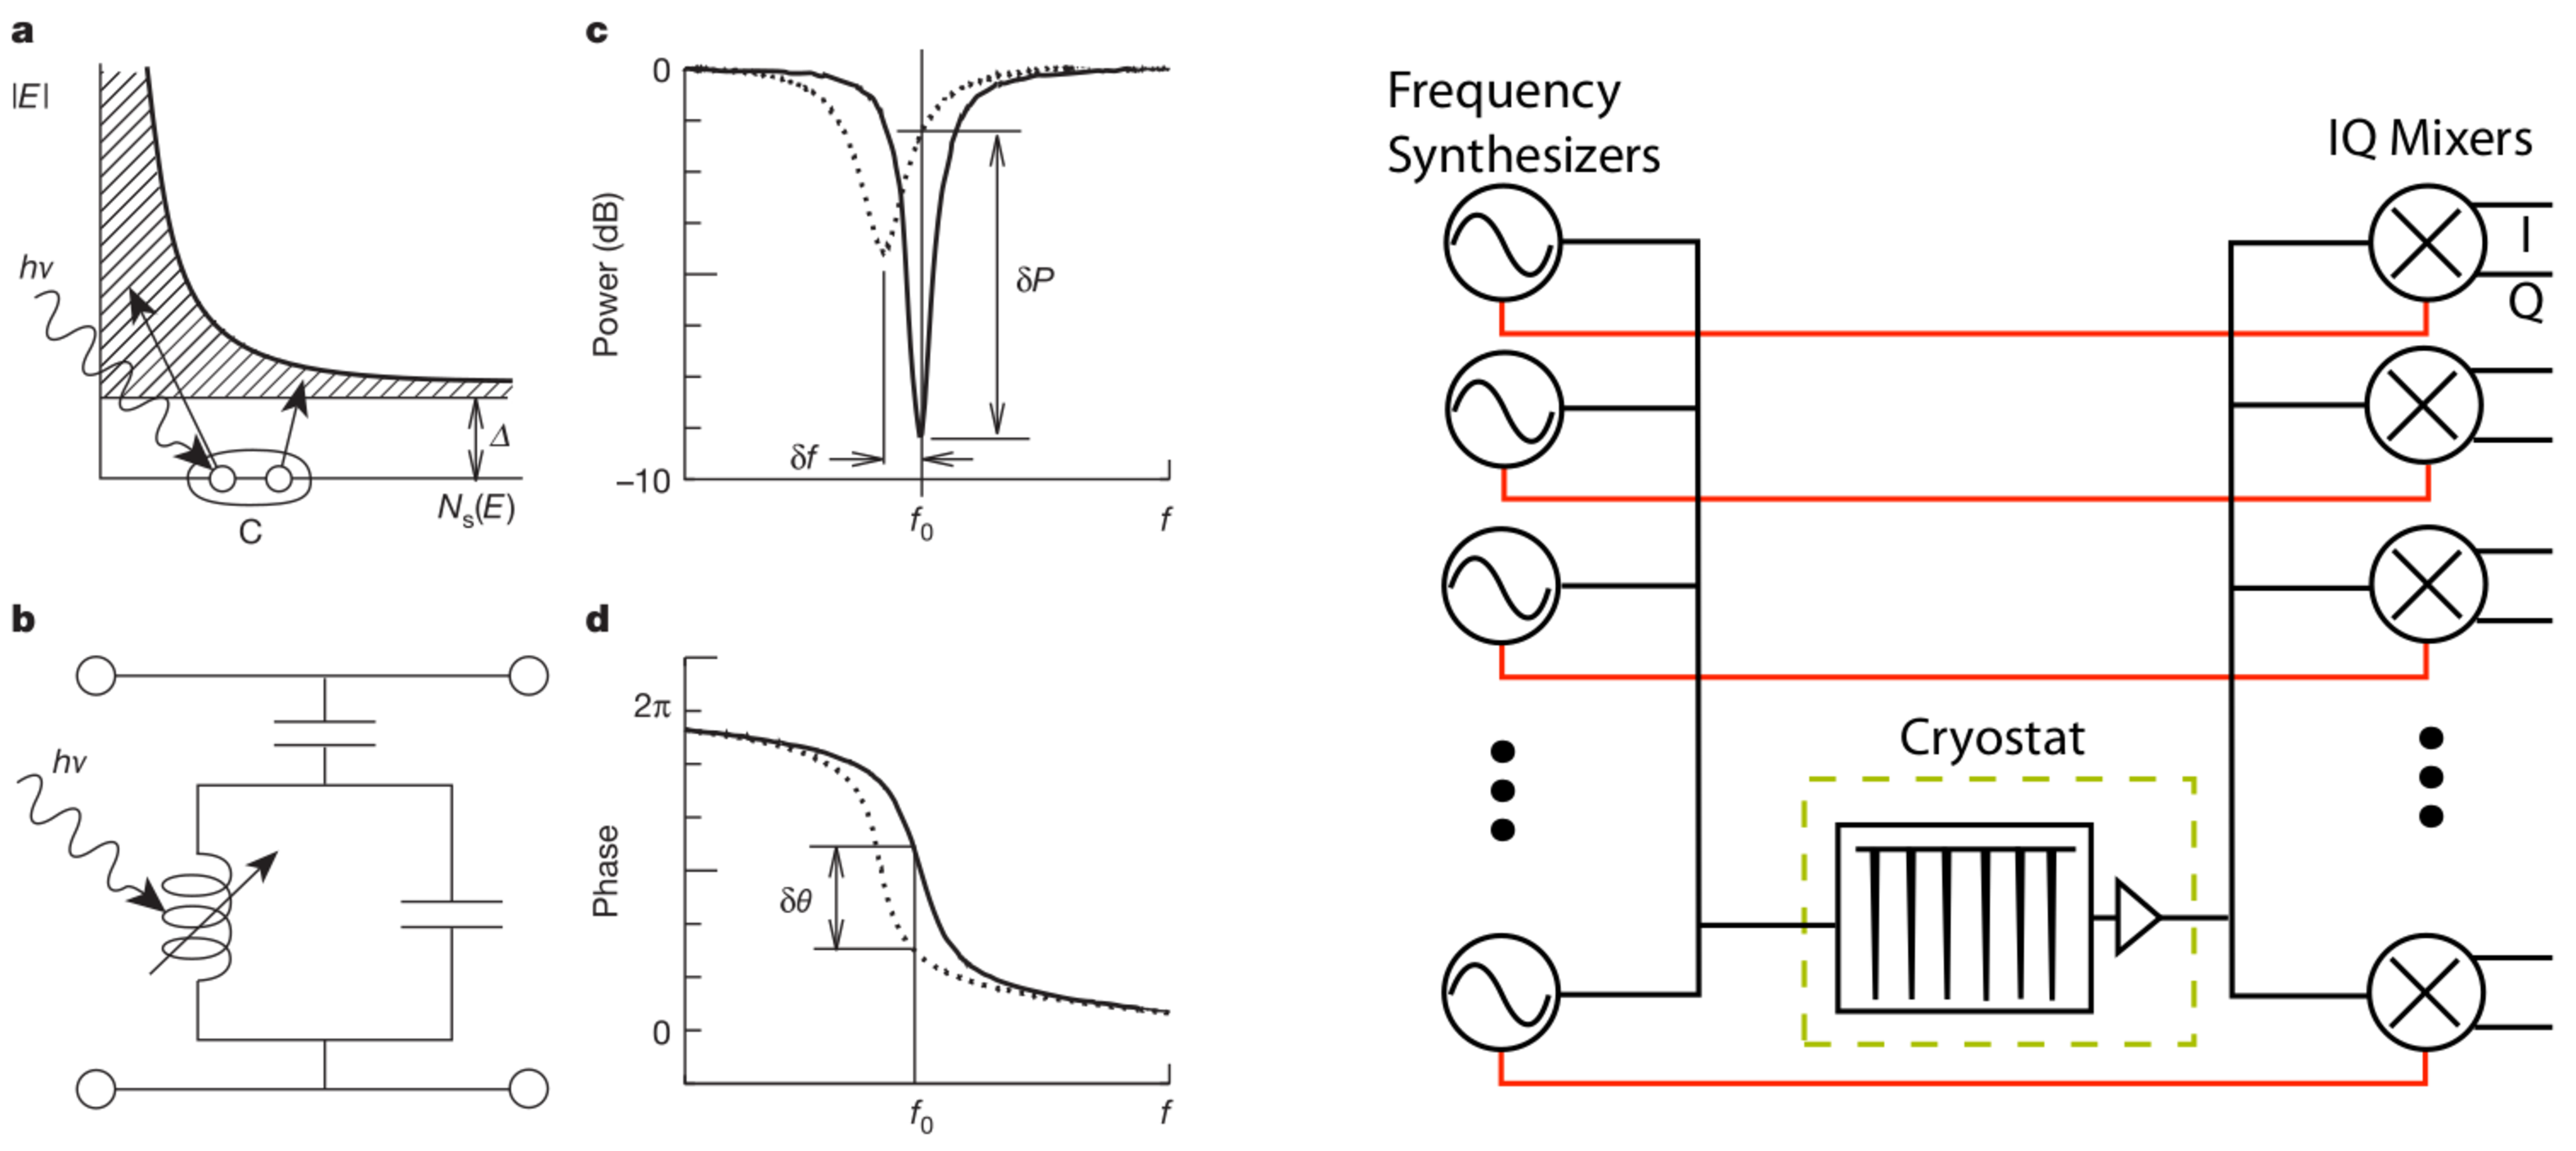
\includegraphics[width=0.8\textwidth]{concepto_mkid1}
				\begin{itemize}
								\item \footnotesize{Superconductores $\to$ inductancia AC debida a la
												inercia de los pares de Cooper}
												\begin{itemize}
																\item[*] \scriptsize{{\color{blue}alternativamente, debido a la
																				energía almacenada en la supercorriente
																				de apantallamiento}}
												\end{itemize}
								\item Cambia cuando los pares de Cooper se rompen debido a la
												energía de entrada
								\item Se mide el cambio monitoreando un circuito resonante
								\item Punto crítico $\to$ los superconductores proveen un muy
												alto Q ($Q_i > 10^7$), así, miles de resonadores
												pueden ser monitoreados a través de una sola linea 
												\begin{itemize}
																\item[*] \scriptsize{{\color{blue}componentes de lectura criogénica muy
																				simples}}
												\end{itemize}
				\end{itemize}

\end{frame}

\begin{frame}{MKID}
				\begin{itemize}
								\item Los MKID funcionan según el principio de que los fotones
												incidentes \alert{cambian la impedancia de la superficie de un
												superconductor a través del efecto de inductancia
												cinética} (Mattis y Bardeen, 1958).
								\item 
								\item ¿Qué beneficios obtengo/obtenemos?
								\item ¿Qué grupos integro/se formaron con esto?
								\item 
								\item 
				\end{itemize}

\end{frame}

\begin{frame}{MKIDs}
				\begin{columns}
								\begin{column}{0.49\textwidth}
												\centering
												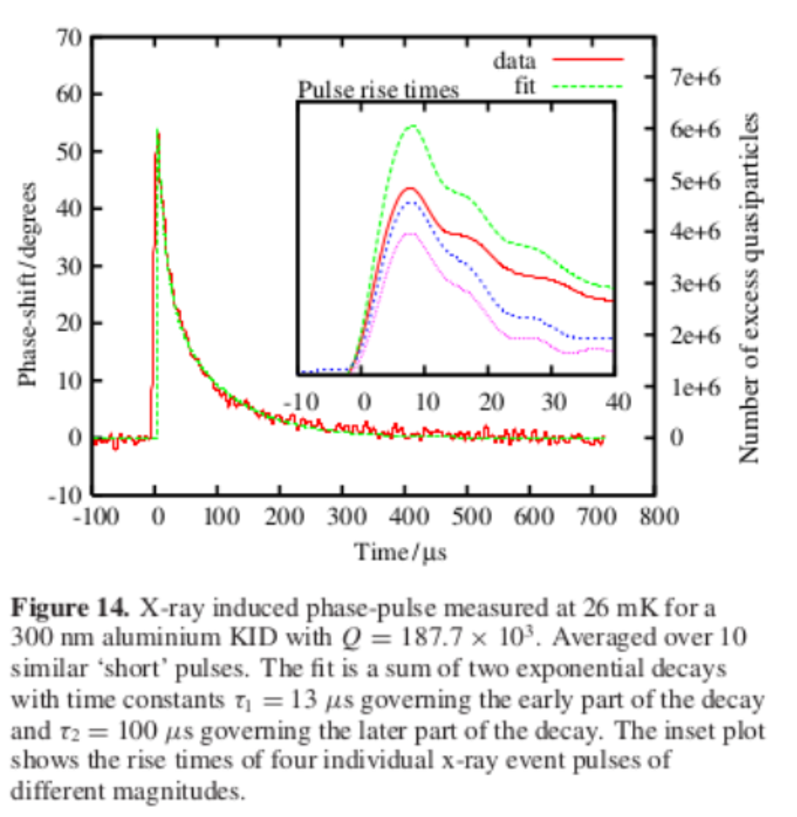
\includegraphics[width=0.92\textwidth]{pulso_respuesta_mkid2}
								\end{column}
								\begin{column}{0.59\textwidth}
												\footnotesize{Mecanismo de detección de los KIDs $\to$ un
												cambio temporal en la inductancia cinética superficial
												de un superconductor cuando se absorbe un fotón de
												energía $h\nu \geq 2 \Delta(T)$, donde $\Delta(T)$ es el
												parámetro de gap superconductor (teoría BCS).
												\pause

												Los fotones de alta energía rompen los pares de Cooper.
												Estos se recombinan en un tiempo característico, del
												orden de $10-500\,\mu\text{s}$,	{\color{red}produciendo
												cambios similares a	pulsos en la impedancia	
												superficial.}
												\pause

												Como la impedancia del superconductor es principalmente
												inductiva, especialmente para $T << T_c$,
												el superconductor puede diseñarse como el elemento
												inductivo en un circuito resonante tipo RLC.
												\pause

												{\color{blue}El factor de calidad (Q) del circuito
												resonante determina ambos, la \alert{sensibilidad} y la
												\alert{velocidad} de respuesta del dispositivo}.}
								\end{column}
				\end{columns}
\end{frame}
\begin{frame}{MKIDs}
				\framesubtitle{Resolución de Energía}
				%\begin{exampleblock}{}
				%       Works on the principle that incident photons change the surface
				%       impedance of a superconductor through the \textit{kinetic
				%       inductance effect}
				%\end{exampleblock}
												\begin{equation*}
																R = \frac{1}{2.355}\sqrt{\frac{\eta h \nu}{F
																\Delta}}
												\end{equation*}
				$\eta = 0.57 \to$ eficiencia para crear cuasipartículas (típico),

				$h\nu \to$ energía del fotón incidente,

				$\Delta = 1.72\,k_BT_c \to$ gap de energía del absorvedor superconductor,

				$F \approx 0.2 \to$ factor de Fano

				$R=150$ a 5\,eV para temperatura de operación de 100\,mK.

				$T = 15$\,mK $\to$ resolución de energía máxima teórica de \alert{$R = 400$ a
				5\,eV} (aunque es probable que otras fuentes de ruido, como el ruido de
				dos niveles del sistema (TLS), sean más importantes a medida que el
				desarrollo futuro aumente	la resolución de energía).

\end{frame}
\begin{frame}{MKIDs}
				\scriptsize{\begin{itemize}
								\item Como detector de fotones en el rango mm/submm
								\item Resonancia  $1-10\,\text{GHz}$
								\item $Q \sim 10^5$
								\item $T_{op} < 300\,\text{mK}$
								\item Resolución de energía intrínseca $R = \frac{E}{\Delta E} \sim
												20-150$\footnote{Rev.Sci.Instr. 83, 044702 (2012)}
								\item Resonadores diseñados para operar separados por 2\,MHz en
												un BW de $4-5\,\text{GHz}$.
								\item Transmisión fuera de resonancia $\simeq 1$
				\end{itemize}
				Cada resonador tendrá un $BW \sim 200\,\text{kHz}$ (\alert{basado en el
				factor de calidad que necesitamos}), se requiere una separación de
				2\,MHz entre los resonadores (la posición del resonador se moverá en
				función de una carga diferente. Si los empaquetamos demasiado cerca uno
				del otro, su posición relativa puede cambiar durante la observación o
				en diferentes ciclos de refrigerado).

				Por lo tanto, queremos que ADC tenga BW de al menos 400\,MHz y una SNR
				superior a 59\,dB.

				Si solo consideramos el ruido de cuantización, teóricamente, una SNR de
				59\,dB requerirá que el ADC tenga al menos 10 bits.
				}
				\tiny{\textbf{arXiv:1310.5891v2 (2013)}}
\end{frame}
\begin{frame}{Tipos de MKIDs}
				\begin{itemize}
								\item OLE Doyle et.al 2008
								\item ¿Por qué lo hago?
								\item ¿Qué beneficios obtengo/obtenemos?
								\item ¿Qué grupos integro/se formaron con esto?
								\item 
								\item 
				\end{itemize}

\end{frame}

%------------------------------------------------------------------------------
\section{Aplicaciones}
\begin{frame}{Polarización del CMB}
				\begin{itemize}
								\item OLE Doyle et.al 2008
								\item ¿Por qué lo hago?
								\item ¿Qué beneficios obtengo/obtenemos?
								\item ¿Qué grupos integro/se formaron con esto?
								\item 
								\item 
				\end{itemize}

\end{frame}

\begin{frame}{Antenna-Coupled multicolor MKIDs}
				\begin{itemize}
								\item OLE Doyle et.al 2008
								\item ¿Por qué lo hago?
								\item ¿Qué beneficios obtengo/obtenemos?
								\item ¿Qué grupos integro/se formaron con esto?
								\item 
								\item 
				\end{itemize}

\end{frame}

\begin{frame}{Detección de fonones usando MKIDs}
				\begin{itemize}
								\item OLE Doyle et.al 2008
								\item ¿Por qué lo hago?
								\item ¿Qué beneficios obtengo/obtenemos?
								\item ¿Qué grupos integro/se formaron con esto?
								\item 
								\item 
				\end{itemize}

\end{frame}

%------------------------------------------------------------------------------
\section{Readout design and development}
\begin{frame}{Diseño y desarrollo del sistema de lectura}
				\framesubtitle{Temas a considerar}

					{\color[rgb]{0.8,.4,.5} ``The readout electronics have the general task
					of performing multiple real-time complex microwave transmission
					measurements, in order to monitor the instantaneous resonance frequency
					and dissipation of the superconducting microresonators that serve as
					mm/submm photon detectors''.}\\

				\tiny{\emph{\textbf{An open-source readout for MKIDs}}, Proc. SPIE Astron.
				Telesc.  Instrum., doi:10.1117/12.856832}

				\normalsize{\begin{itemize}
								\item Algoritmo de procesamiento de señal digital en FPGA
								\item Selección de frecuencia, velocidad de datos de salida
								\item Ruido
								\item Rango dinámico
								\item Frecuencias espúreas, productos de intermodulación, etc.
								\item Detalles de implementación: ubicación, empaque, fuente de
												energía, comunicación, interfaz de computadora, etc.
				\end{itemize}}
\end{frame}
\begin{frame}{Diseño y desarrollo del sistema de lectura}
				\centering
				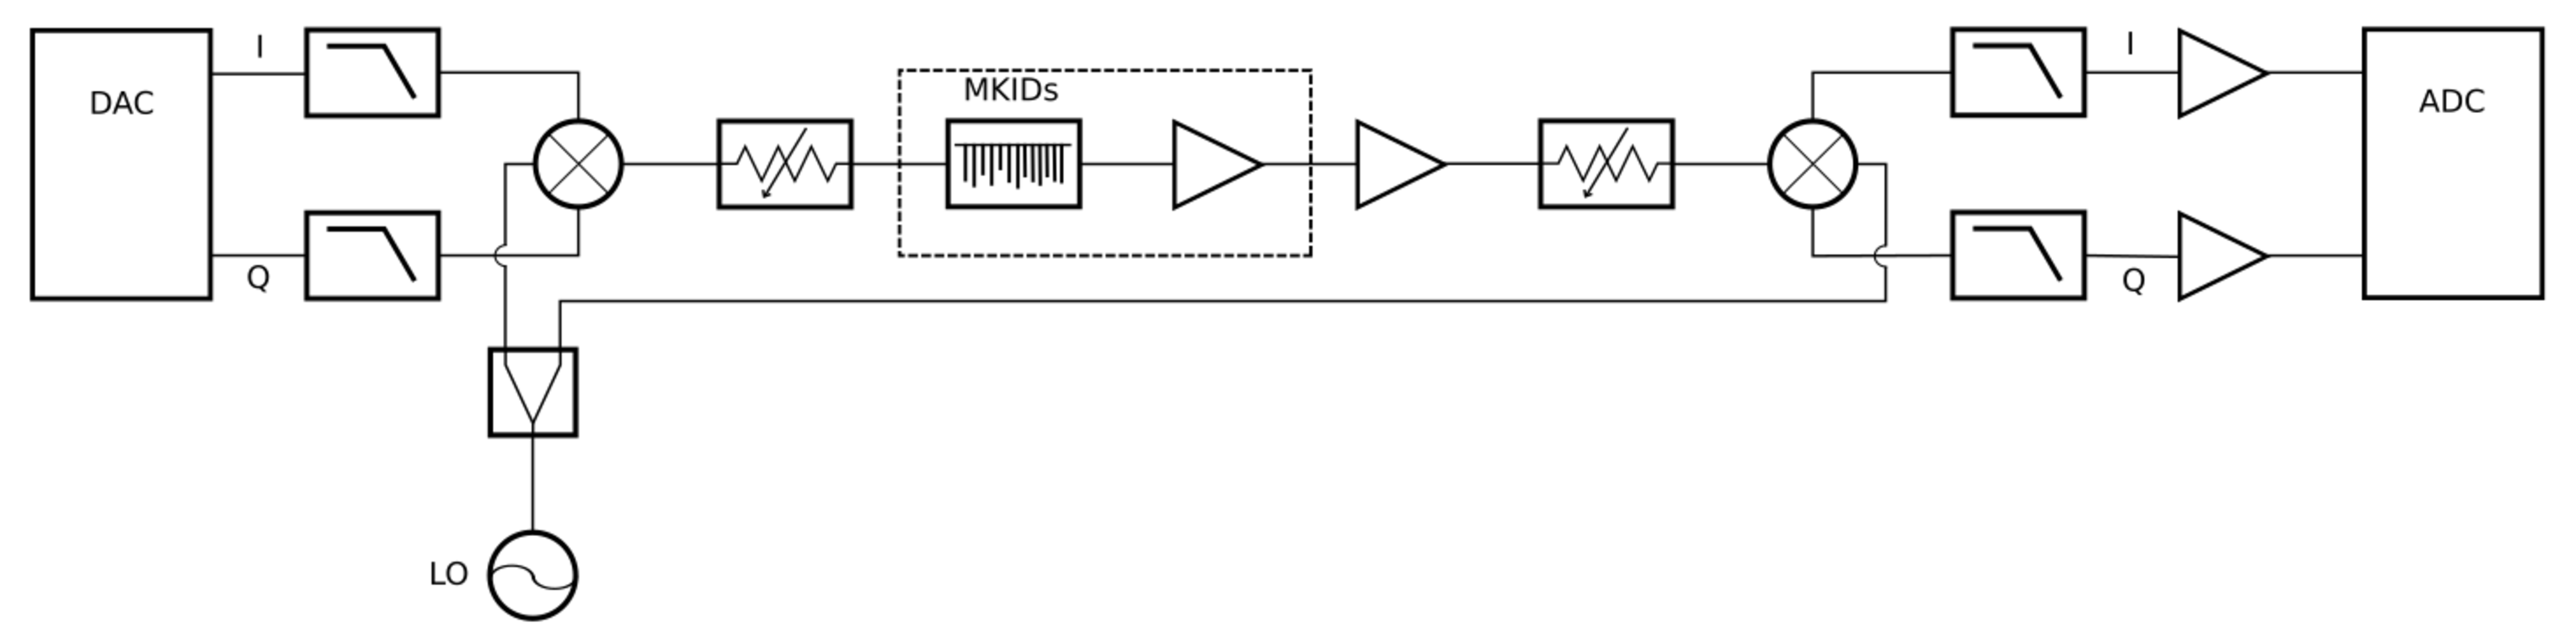
\includegraphics[width=\textwidth]{readout1}

				\begin{itemize}
								\item El ruido estará \alert{dominado por el amplificador
												criogénico (AC)},	el cual tiene una temperatura de ruido
												alrededor de 2 a 5\,K. 
								\item Además del AC, \alert{el chip ADC será el próximo factor
												limitante para el ruido de lectura}.
								\item	En función del espaciado de frecuencia física de todos los
												resonadores, \alert{la frecuencia de muestreo se elige para que
												coincida con el ancho de banda del resonador}.
								\item	La frecuencia de muestreo del sistema propuesto debe ser
												{\color[rgb]{0.2,0.9,0.3}flexible}.  
												%	Right now it is up to 550
												%MHz which is the limit of ADC chip.
				\end{itemize}

				%\tiny{\emph{\textbf{An open-source readout for MKIDs}}, Proc. SPIE Astron.
				%Telesc.  Instrum., doi:10.1117/12.856832}
\end{frame}
\begin{frame}{Diseño y desarrollo del sistema de lectura}
				\only<1>{\footnotesize{\begin{itemize}
								\item Para leer un MKID, se pasa un tono de prueba a su
												frecuencia resonante
								\item Cuando el detector absorbe un fotón, la fase del tono
												cambia repentinamente
								\item A partir de este cambio, se determina la \alert{energía} y
												el \alert{tiempo de llegada} del fotón.
								\item En la lectura, los DAC generan un peine de frecuencia
												complejo que se mezcla con el rango de frecuencias
												resonantes
								\item La señal resultante se envía a través de la matriz MKID,
												se mezcla de nuevo a la banda base y se digitaliza
												mediante un ADC
								\item Esto es procesado por el firmware en la FPGA, que detecta
												eventos de fotones en la fase del tono de prueba de cada
												píxel
								\item Los datos de los fotones se envían a una computadora de
												adquisición y control de datos para su registro
				\end{itemize}}}
				\centering
				\only<2>{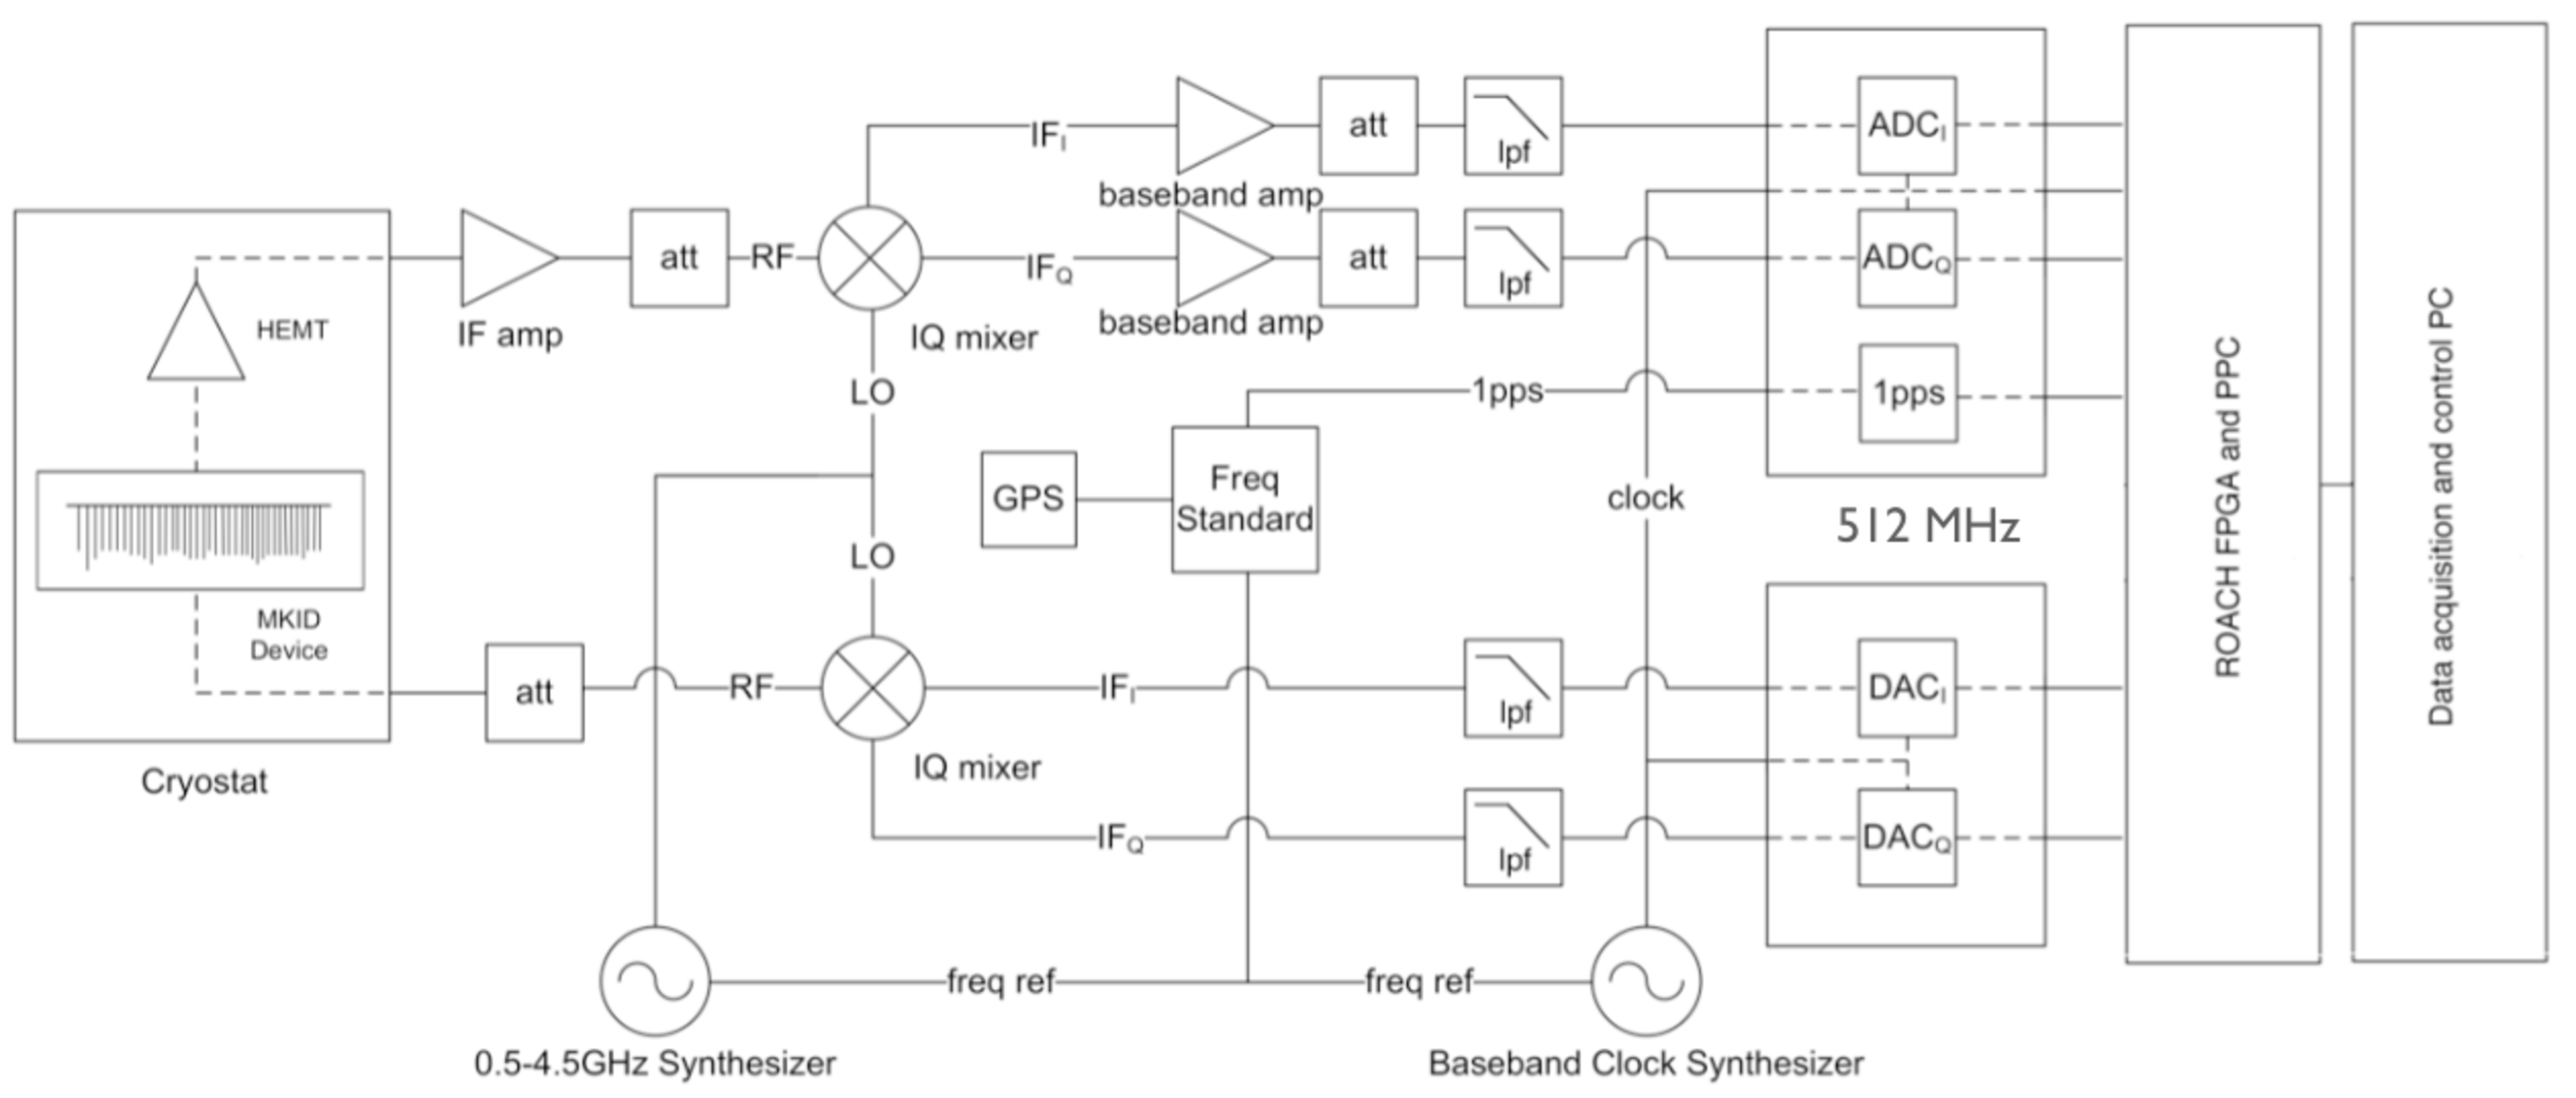
\includegraphics[width=0.8\textwidth]{arcons_readout}}
\end{frame}

\begin{frame}{Firmware}
				The firmware is written in VHDL/Verilog. 

				It controls the DAC output, and processes the ADC input. 

				It separates the digitized readout signal into frequency bins (channels)
				corresponding to each pixel. 

				The signal for each pixel is filtered and converted to phase before
				being run through \alert{pulse detection}.

				The output data rate is expected to be around 100 complex $S_{21}$
				measurements per second, per resonator\footnote{\tiny{from
				MKIDCam Readout Electronics Specifications (2008)}} $\to$ (\alert{to be
				confirmed})
\end{frame}

\begin{frame}{Pulse detection}
				\begin{columns}
								\begin{column}{0.49\textwidth}
												\scriptsize{Readout capable of recording to file one continuous
												second of phase data for one pixel at a time, \alert{sampled at
												1\,MHz}. 

												To record data from all the pixels, though, the firmware must
												reduce the data to only include data from detected photons,
												which are seen as negative peaks in the phase.}
								\end{column}
								\begin{column}{0.49\textwidth}
												\centering
												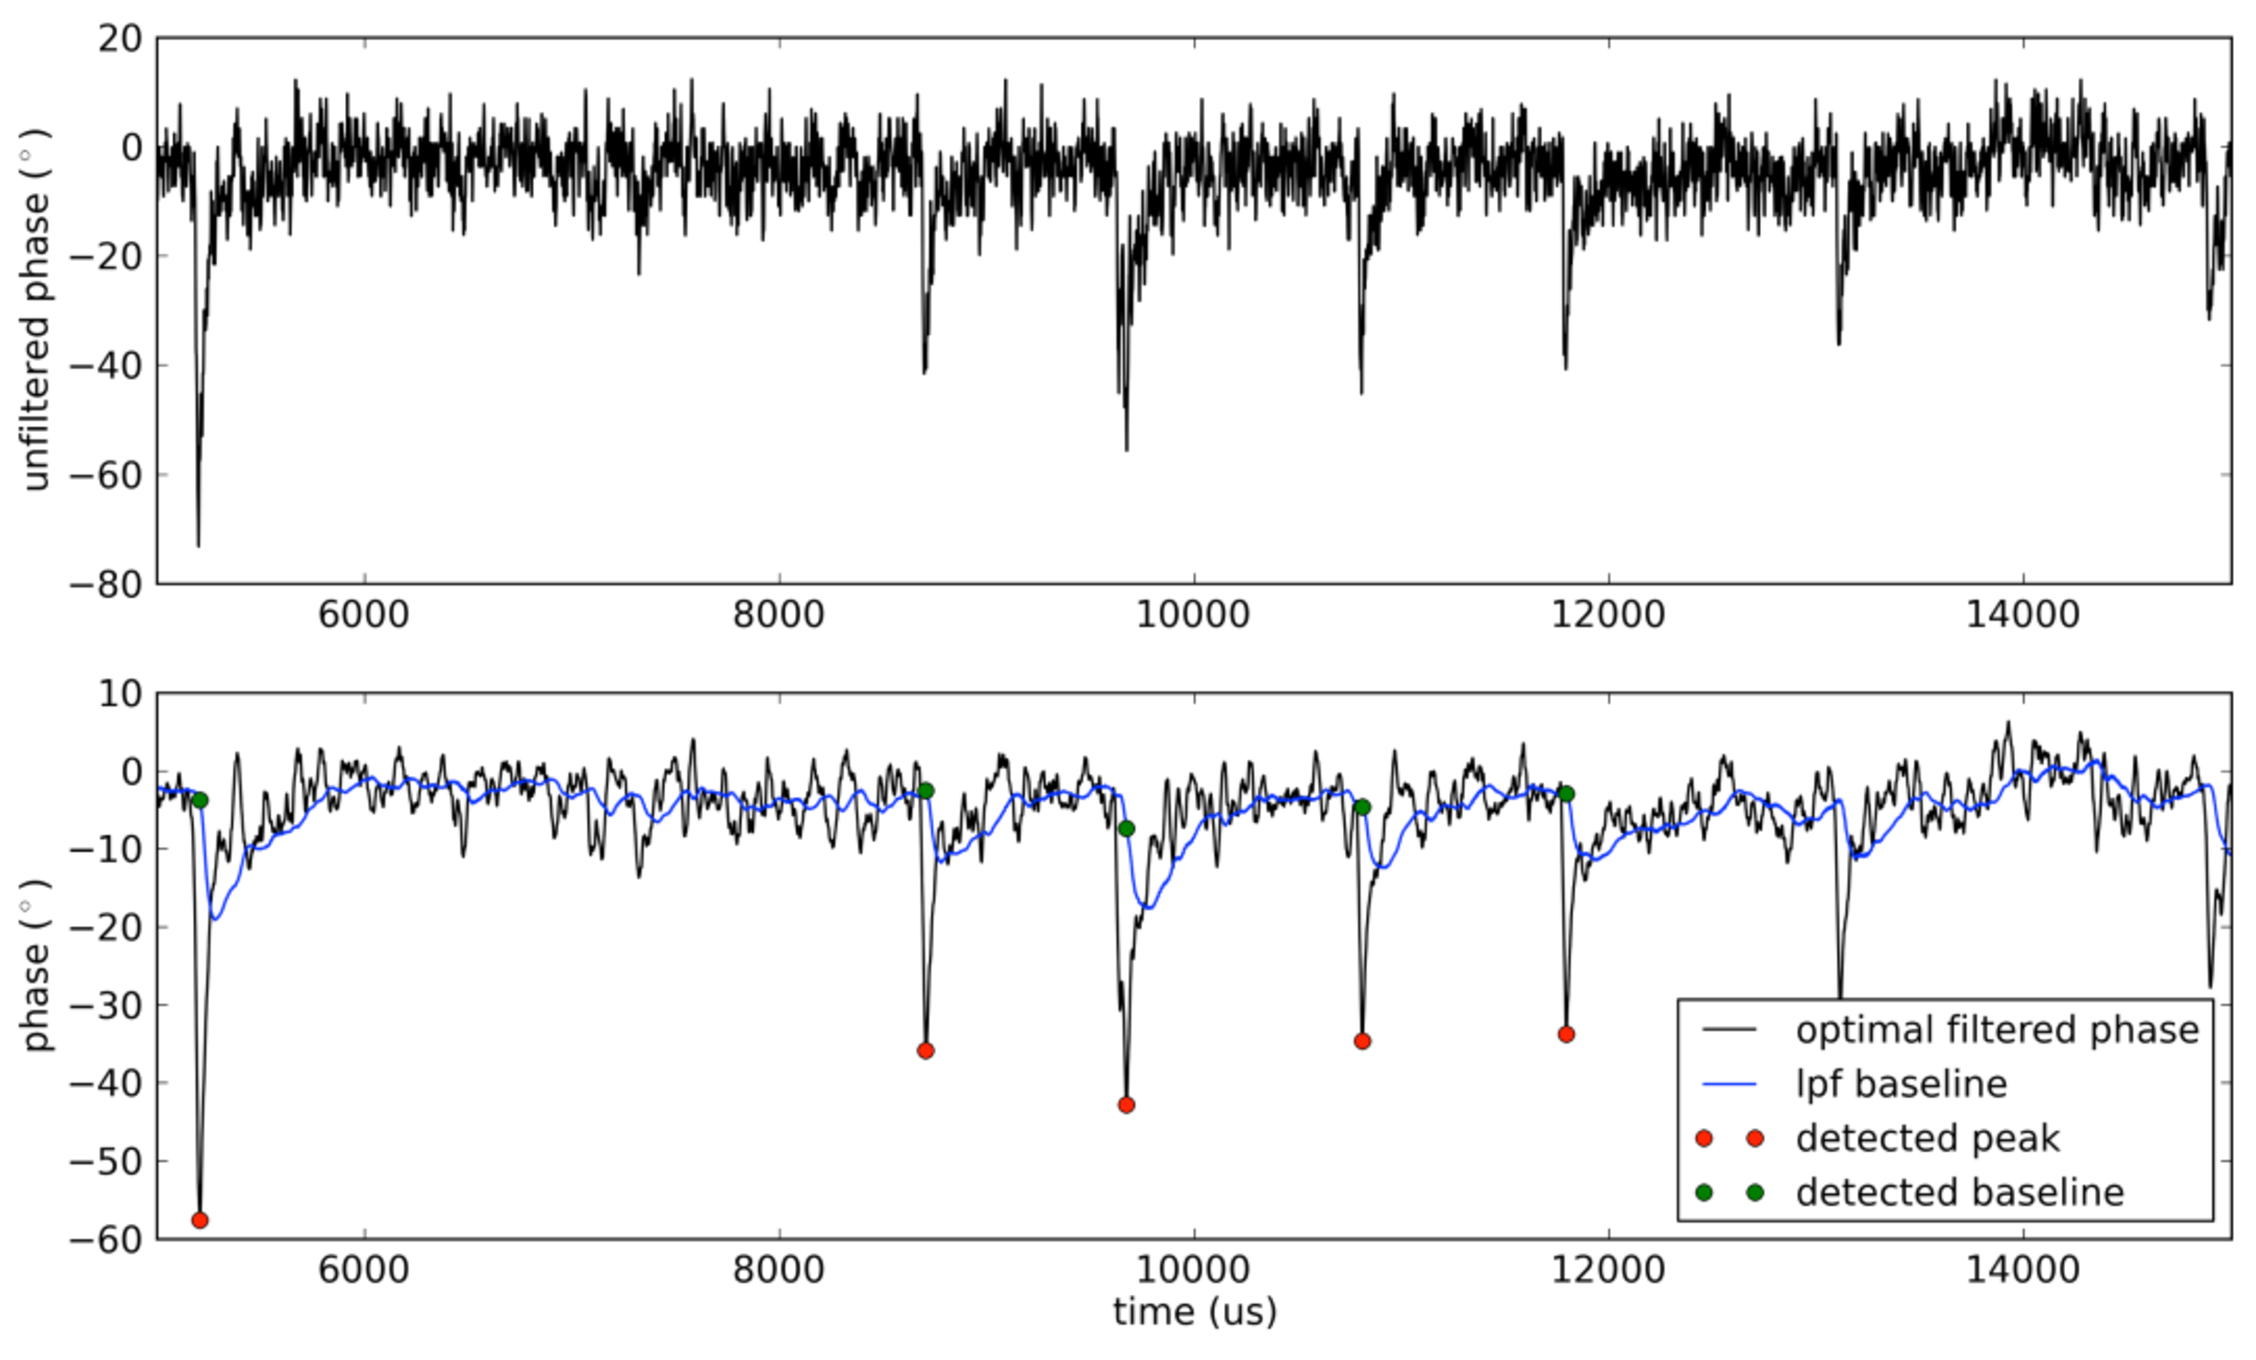
\includegraphics[width=0.98\textwidth]{pulsos_de_fase}
								\end{column}
				\end{columns}
				\scriptsize{A (programmable) filter is applied to the phase signal to increase the
				SNR of drops in phase due to photons.  

				{\color{blue}Snapshots	of raw phase data are used to create a
				\alert{matched filter},	customized to each pixel.}

				The {\color{blue}firmware} also keeps track of the phase baseline and subtracts it
				before checking for photon pulses, to resist false triggers from $1/f$
				noise.\footnote{ARCONS talks.}}
\end{frame}
%\begin{frame}{Readout design and development}
%
%				MKIDs $\to$ 
%
%				The obvious advantage of MKIDs over competing cryogenic technologies
%				like TESs is the elimination of the cryogenic electronics required for
%				multiplexing
%
%				\tiny{\emph{\textbf{A readout for large arrays of microwave kinetic
%				inductance detectors}}, Rev. Sci. Instrum., doi:10.1063/1.3700812}
%\end{frame}

\begin{frame}{Design requirements}
				\begin{itemize}
								\item The readout must not introduce significant noise above the
												system noise floor set by the \textbf{cryogenic
												amplifier} with a noise temperature of $\sim
												4\,\text{K}$.
								\item The entire readout system must be capable of
												reading out at least \alert{512 resonators} in $\sim
												1\,\text{GHz}$ of bandwidth ({\color{red} to be
												confirmed}).
								\item \alert{Crosstalk} between channels greater than
												$250\,\text{kHz}$ apart should be less than \alert{1\%}.
								\item Intrinsic energy resolution \alert{$R \sim 20-150$}
												\footnote{Rev.Sci.Instr. 83, 044702 (2012)}
				\end{itemize}
\end{frame}

\begin{frame}{The cryogenic amplifier}
				%\begin{itemize}
				%\item 
				The double sideband (DSB) phase noise of the HEMT
			amplifier is given by the simple expression, 
			{\color{red}
			\begin{equation*}
							N_{\phi \text{DSB}} = \frac{k_B T_n}{P}
			\end{equation*}} 
			\flushleft
			$T_n \to$ noise temperature of the amplifier, 

			$P \to$ power on the input. 

			The readout power for each MKID should be $-100 \pm
			15\,\text{dBm}$ ({\color{red} to be confirmed}). 

			For	$-85\,\text{dBm}$ readout power, off resonance, and $T_n
			= 6\,\text{K}$, we expect $-106\,\text{dBc/Hz}$ for the
			HEMT phase noise. Ideally, the readout electronics will
			contribute noise well below this
			value.\footnote{Rev.Sci.Instr. 83, 044702 (2012)}
			%\end{itemize}
\end{frame}

\begin{frame}{$N_\text{channels}$ vs. $P_\text{readout}$}
				\footnotesize{\textbf{Rev.Sci.Instr. 83, 044702 (2012)}}
				\begin{columns}
								\begin{column}{0.5\textwidth}
												\begin{itemize}
																\item \footnotesize{Dada la especificación de
																				ruido de voltaje del ADC, se puede
																				calcular el número de canales
																				{\color{blue}$n$} que el ADC puede leer
																				a una potencia dada sin aumentar el
																				ruido del HEMT (amplificador)}
																\item Los contornos de la Fig. 3 se calculan
																				escalando  el ruido del HEMT con un
																				factor dependiente del canal, $k_B
																				T_n /(p_\text{max}^2 P)$.
																\item $p_\text{max} \propto
																				n^{1/2}\quad\text{para}\quad n >> 1$
																\item Se asume fase aleatoria por tono
												\end{itemize}
								\end{column}
								\begin{column}{0.5\textwidth}
												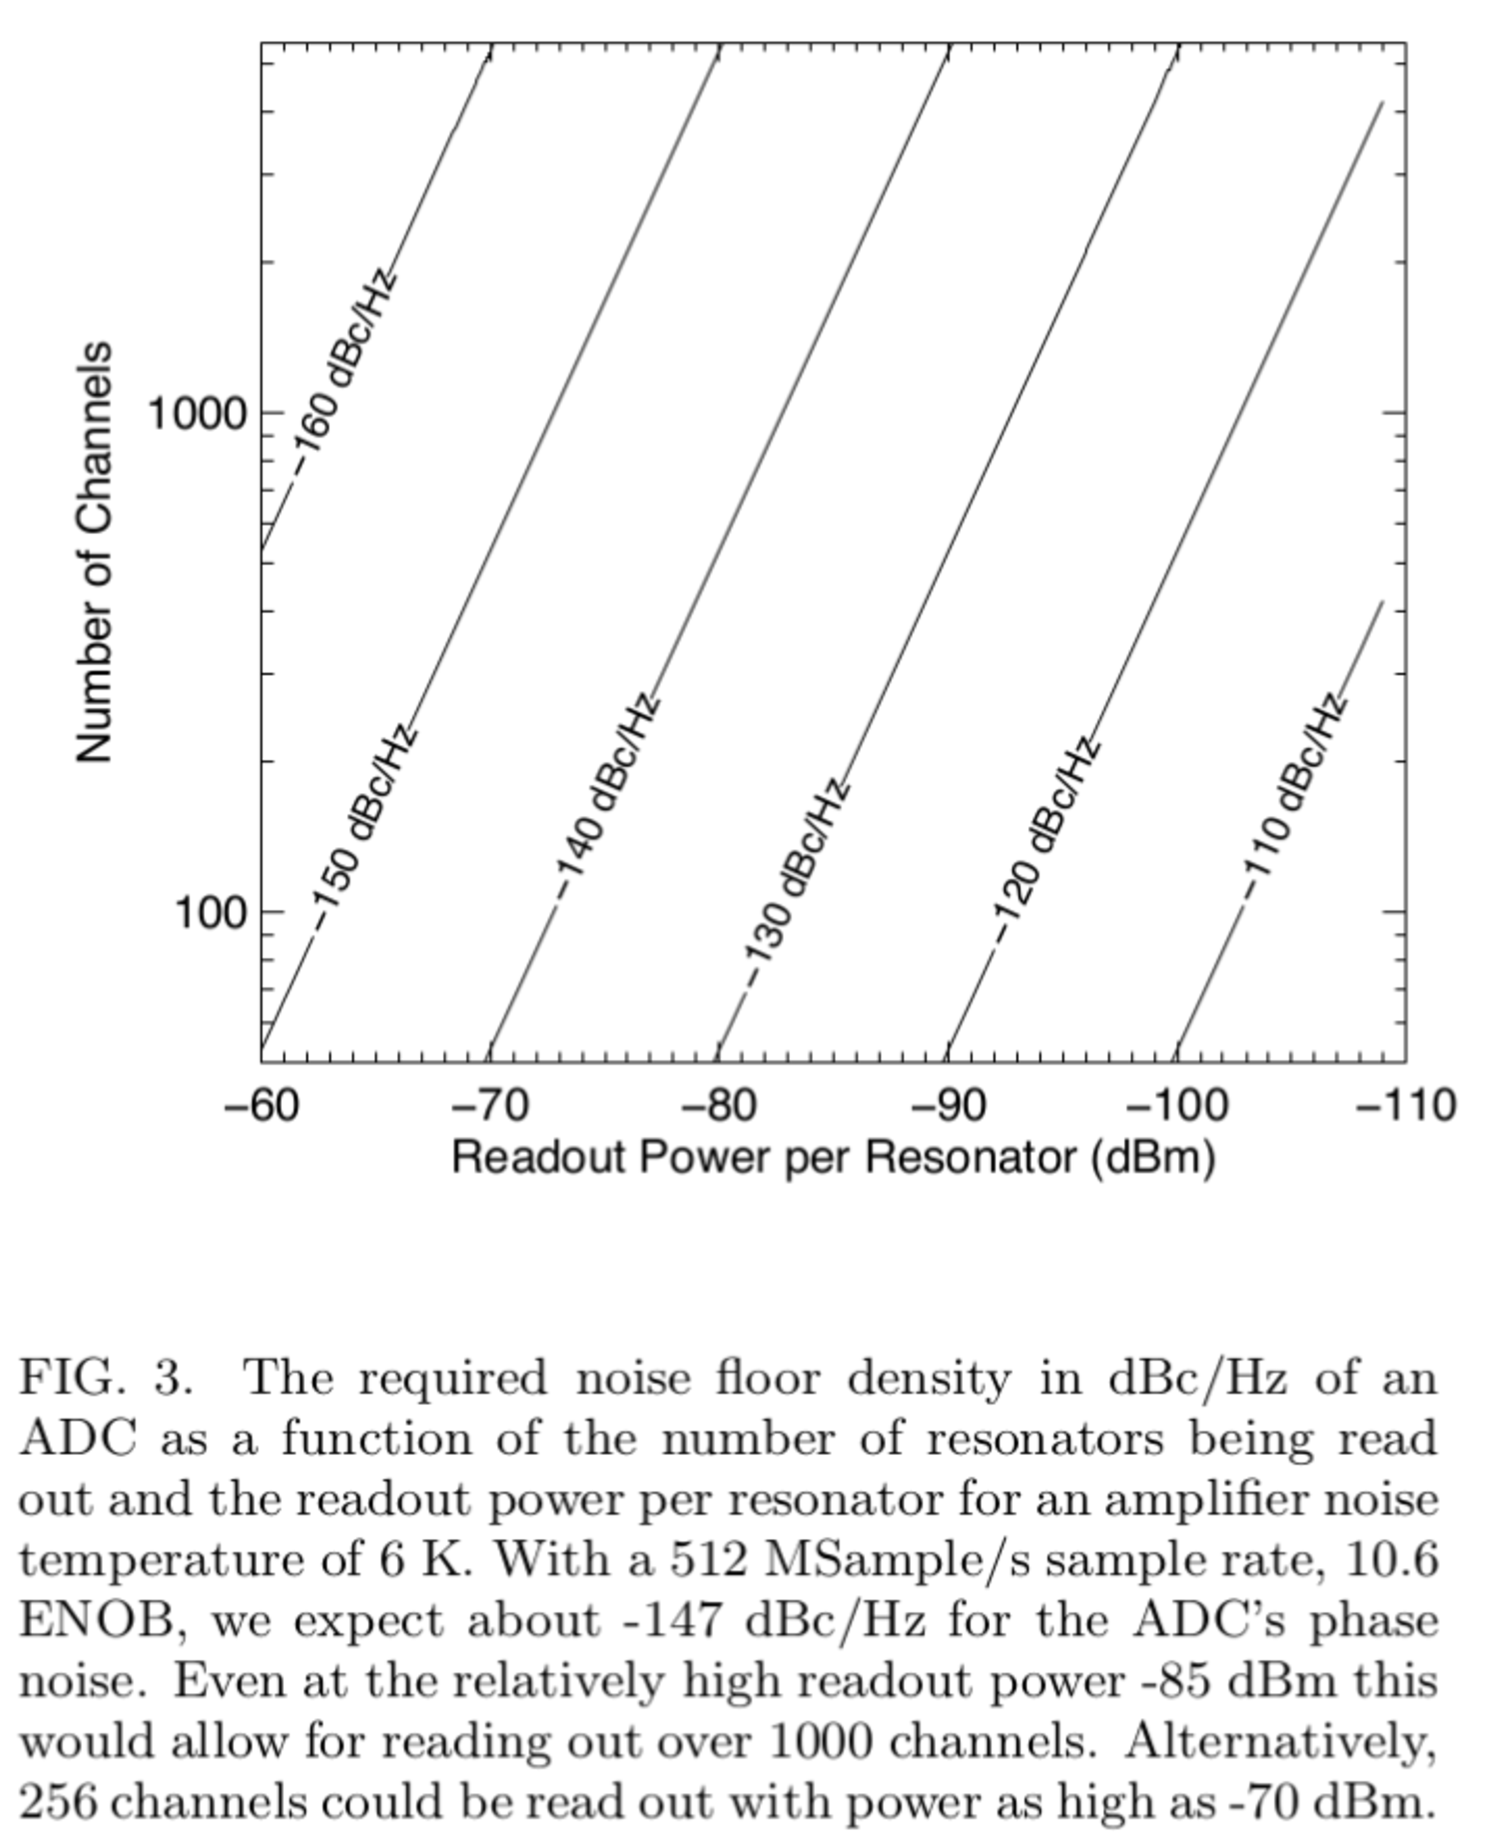
\includegraphics[width=0.95\textwidth]{power_vs_Nchannels}
								\end{column}
				\end{columns}
\end{frame}

%------------------------------------------------------------------------------
%------------------------------------------------------------------------------
\section{ARCONS}
\begin{frame}{ARCONS}

				\textbf{A}rray \textbf{C}amera for \textbf{O}ptical to \textbf{N}ear-IR
				\textbf{S}pectrophotometry
				\begin{itemize}
								\item Primer instrumento terrestre basado en MKIDs para el rango de
												longitud de onda óptica hasta el IR cercano
								\item Diseño óptico simple que permite muy alto rendimiento
								\item Resolución de tiempo de hasta seis órdenes de magnitud
												mejor que un CCD
								\item Ancho de banda intrínseco extremadamente amplio (0.1
												-5\,$\mu$m) con buena eficiencia cuántica
								\item Sin ruido de lectura o corriente oscura, y casi perfecto
												rechazo de rayos cósmicos
								\item No se pierde tiempo de observación al leer la matriz
				\end{itemize}

				%\begin{center}
				%				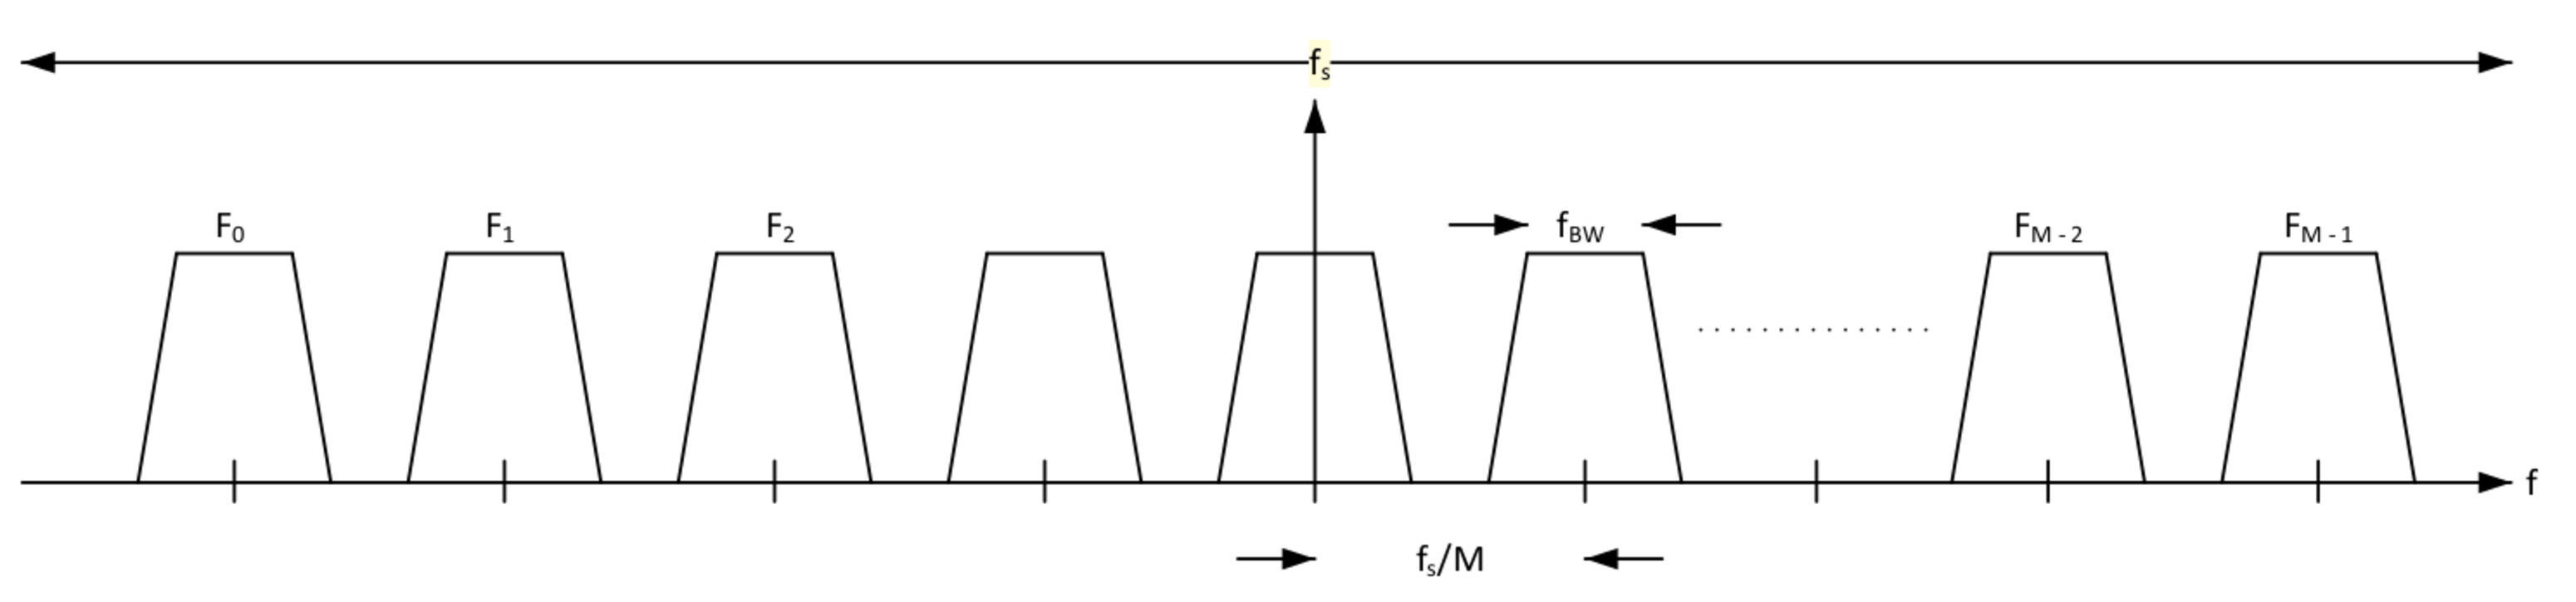
\includegraphics[width=0.8\textwidth]{FDM_channel_diagram}
				%\end{center}
\end{frame}
\begin{frame}{ARCONS}

				\textbf{A}rray \textbf{C}amera for \textbf{O}ptical to \textbf{N}ear-IR
				\textbf{S}pectrophotometry
				\begin{itemize}
								\item La tecnología actual óptica MKID tiene una resolución
												espectral $R = \lambda/\Delta \lambda \sim 10$ a
												\SI{4000}{\angstrom}
								\item 
								\item Resolución de tiempo de hasta seis órdenes de magnitud
												mejor que un CCD
								\item Ancho de banda intrínseco extremadamente amplio (0.1
												-5\,$\mu$m) con buena eficiencia cuántica
								\item Sin ruido de lectura o corriente oscura, y casi perfecto
												rechazo de rayos cósmicos
								\item No se pierde tiempo de observación al leer la matriz
				\end{itemize}

				%\begin{center}
				%				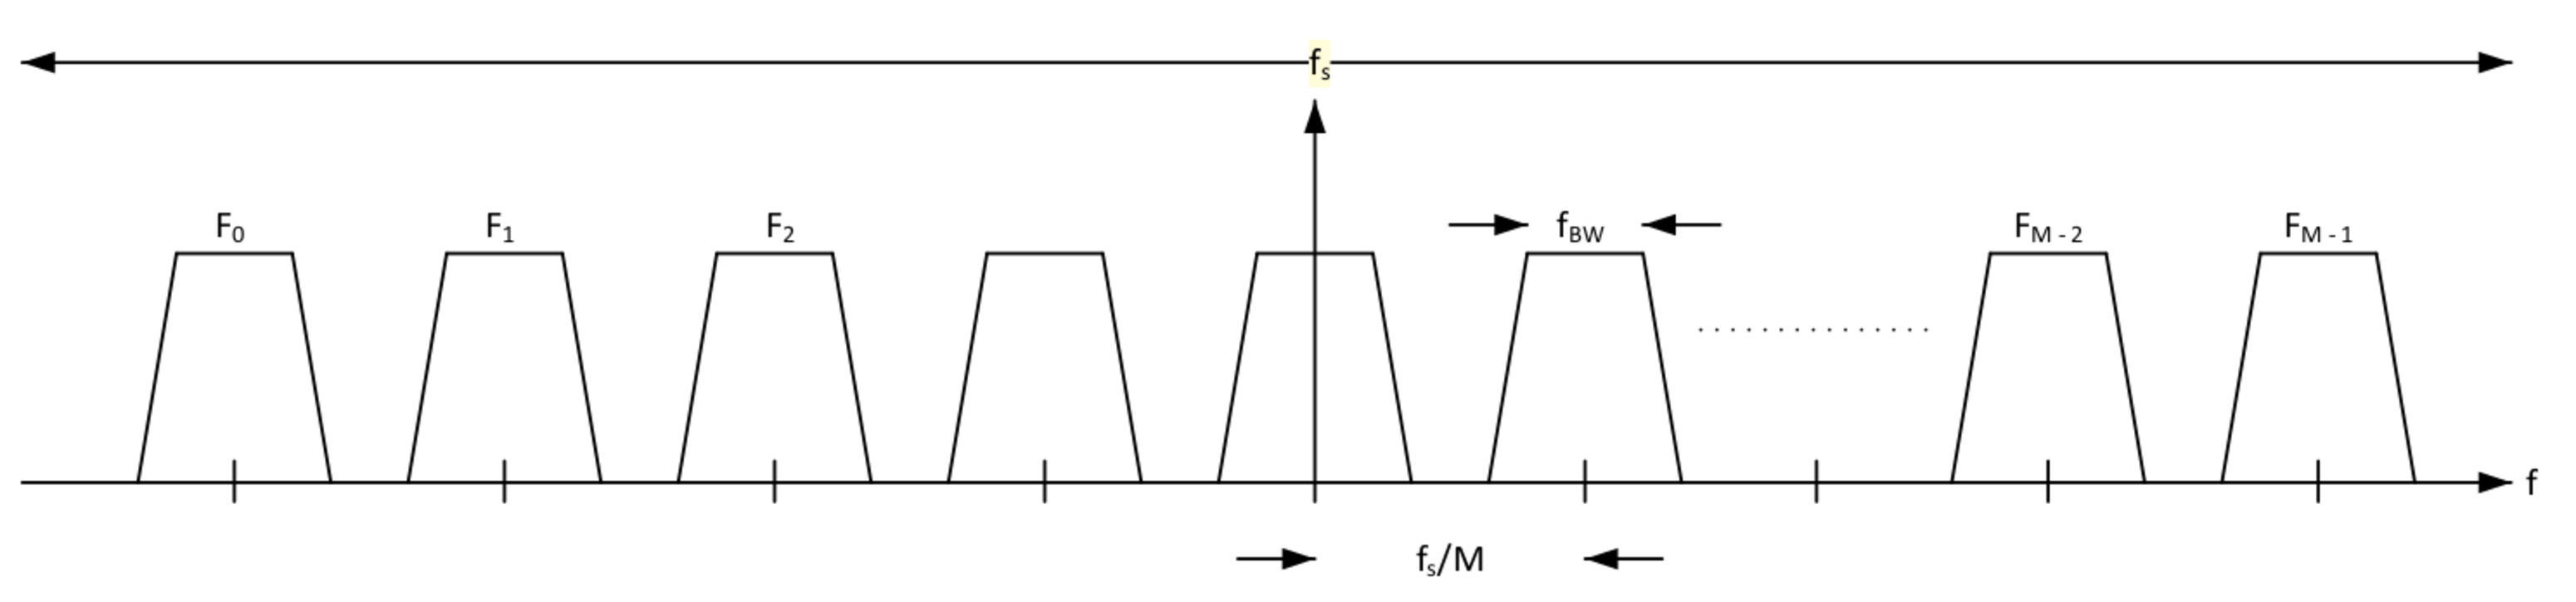
\includegraphics[width=0.8\textwidth]{FDM_channel_diagram}
				%\end{center}
\end{frame}

%------------------------------------------------------------------------------
\section{FDM}
\begin{frame}{Frequency Division Multiplexing (FDM)}
				\begin{columns}
								\begin{column}{0.5\textwidth}
												\begin{itemize}
																\item[o]	Estrategia de multiplexación poderosa\\
												\qquad --\footnotesize{Muchos detectores están acoplados
												a una sola linea}
								\normalsize{\item[o] Muchos canales por amplificador de microondas
								\item[o] Hardware criogénico: solo un amplificador y algunos
												cables coaxiales}
												\end{itemize}
				\begin{center}
								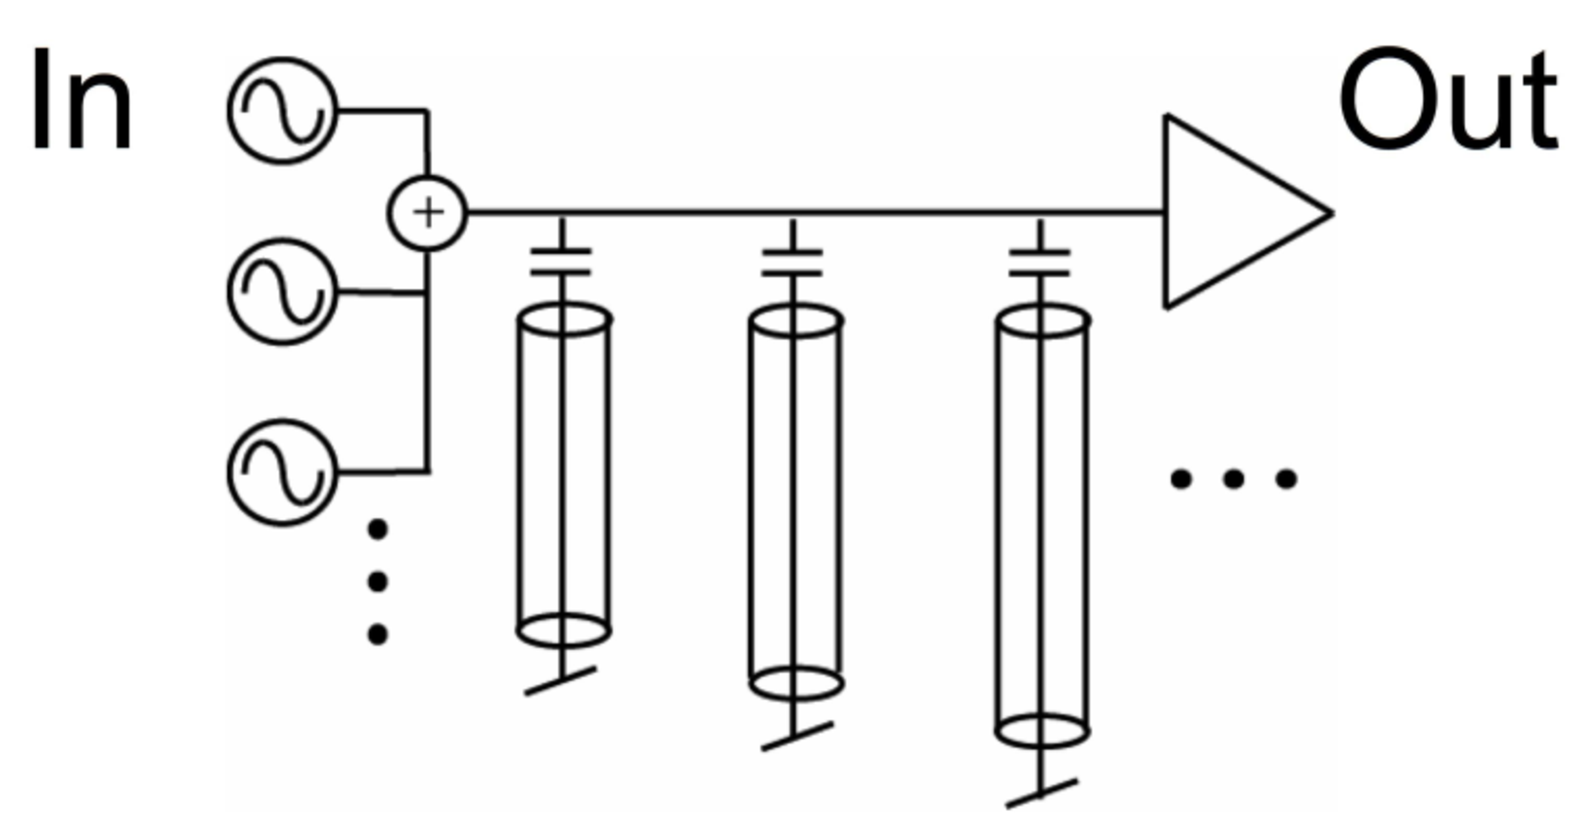
\includegraphics[width=\textwidth]{fdm1}
				\end{center}
								\end{column}
								\begin{column}{0.5\textwidth}
								\begin{center}
												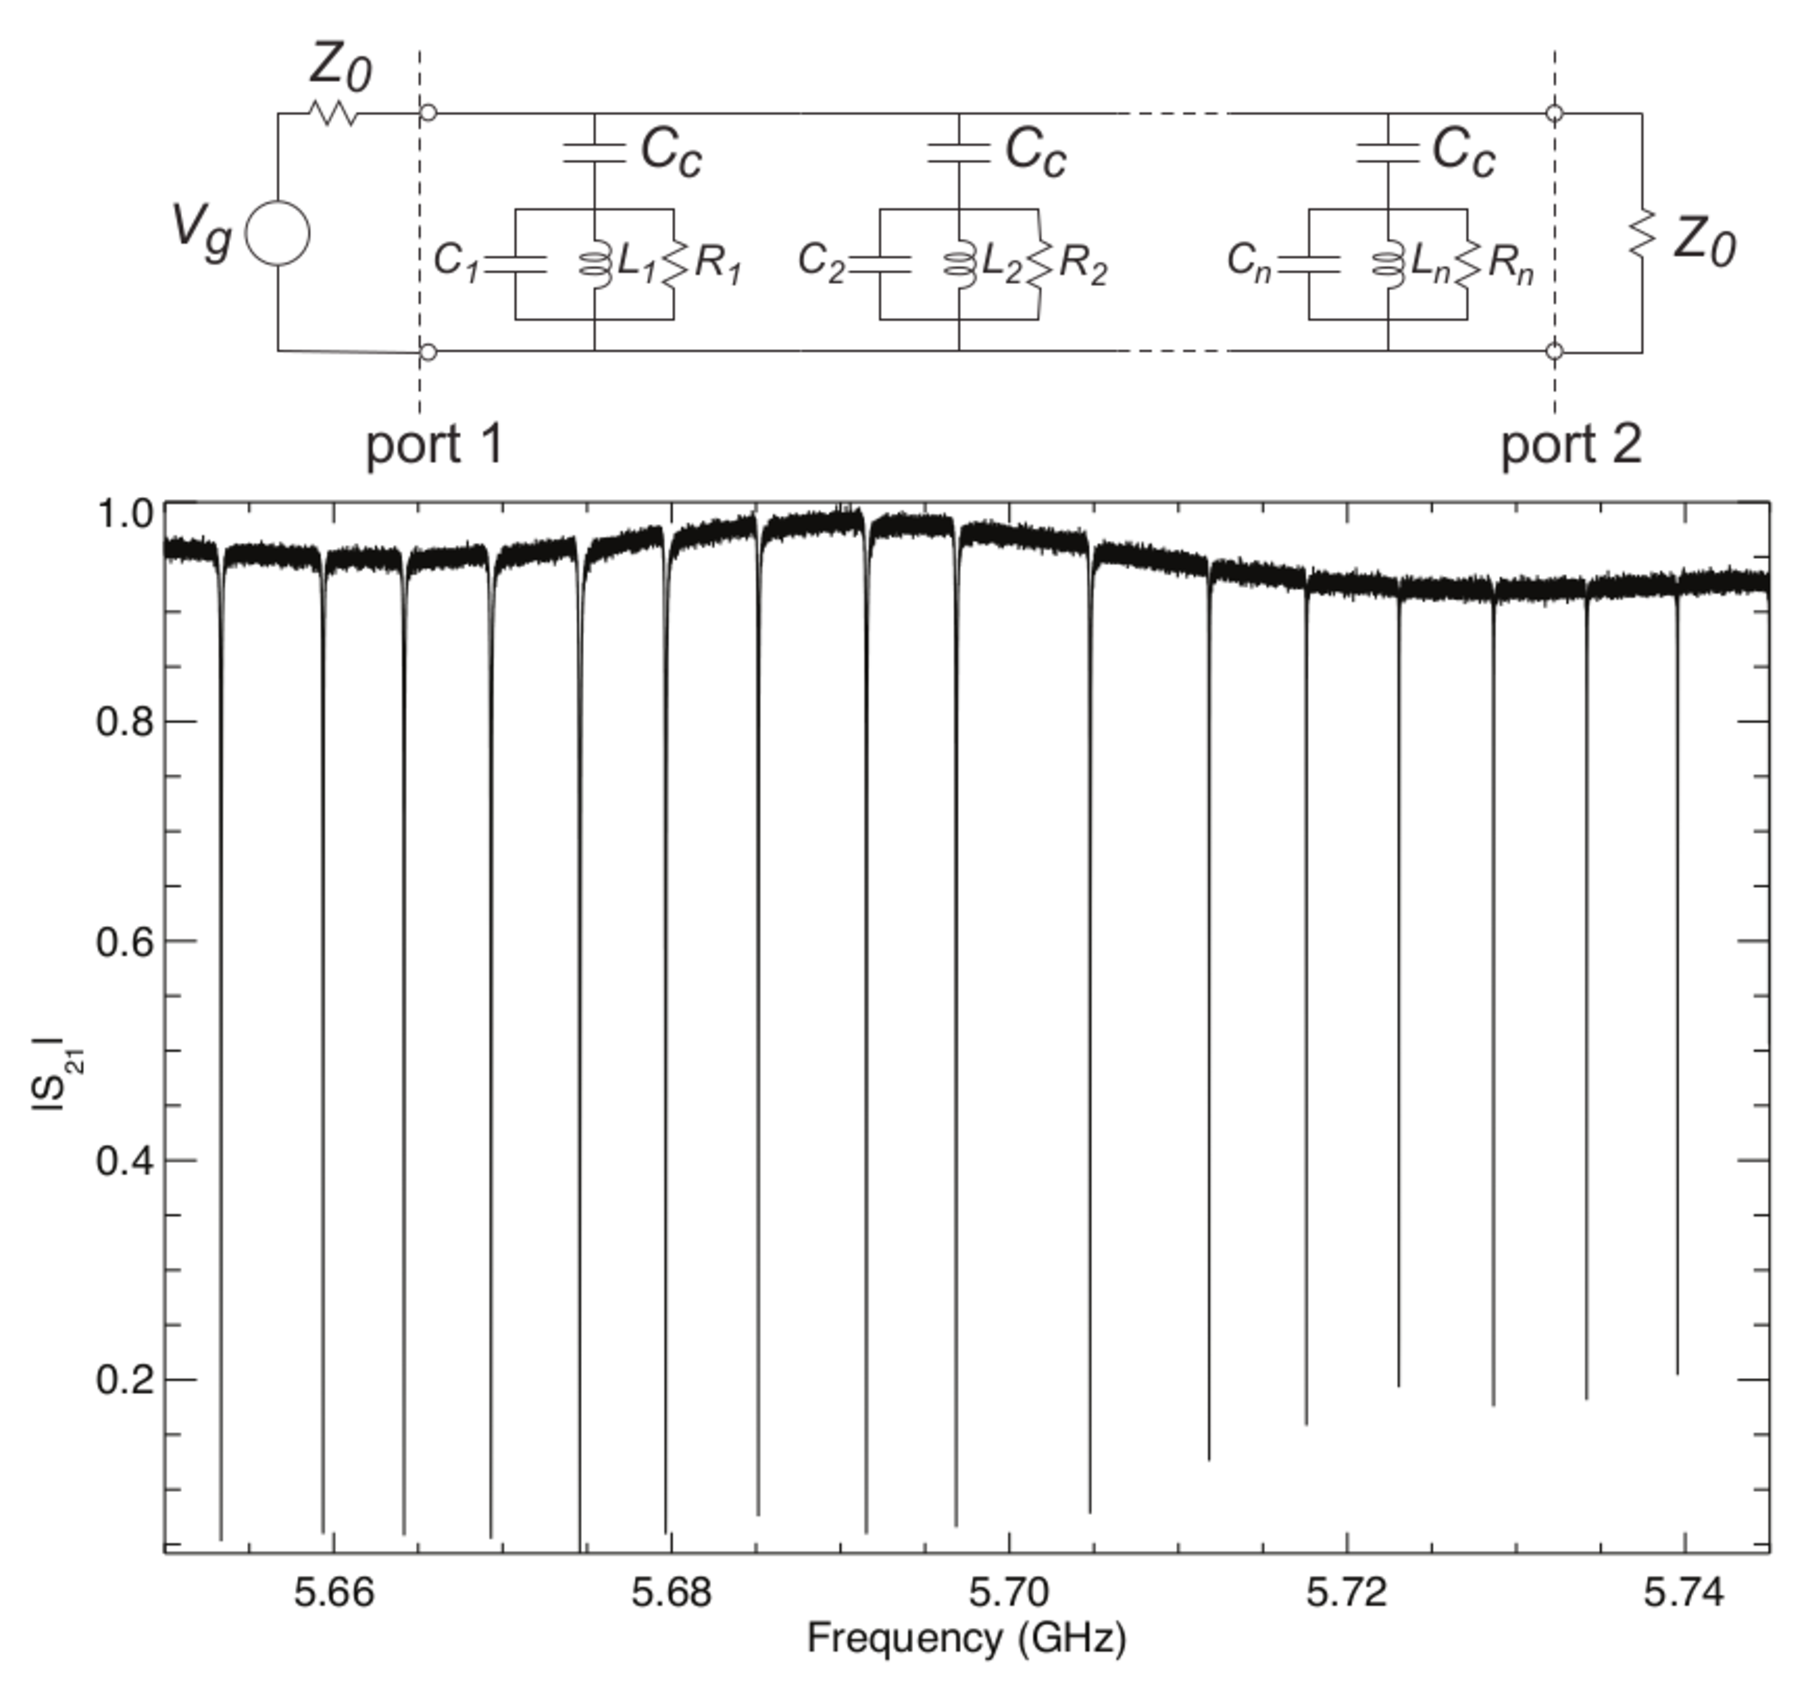
\includegraphics[width=\textwidth]{fdm2}
								\end{center}
												\end{column}
								\end{columns}

\end{frame}

%------------------------------------------------------------------------------
\section{Firmware: Channelizer}

\begin{frame}{Canalizador DFT (Channelizer)}

				Implementación m\'as eficiente en t\'erminos de uso de hardware en FPGA

				Ancho de banda similar para todos los canales 

				Extensible a un n\'umero grande de canales ($>=1000$)

				Posibilidad de realizar el diseño en multi-etapas

				\begin{center}
								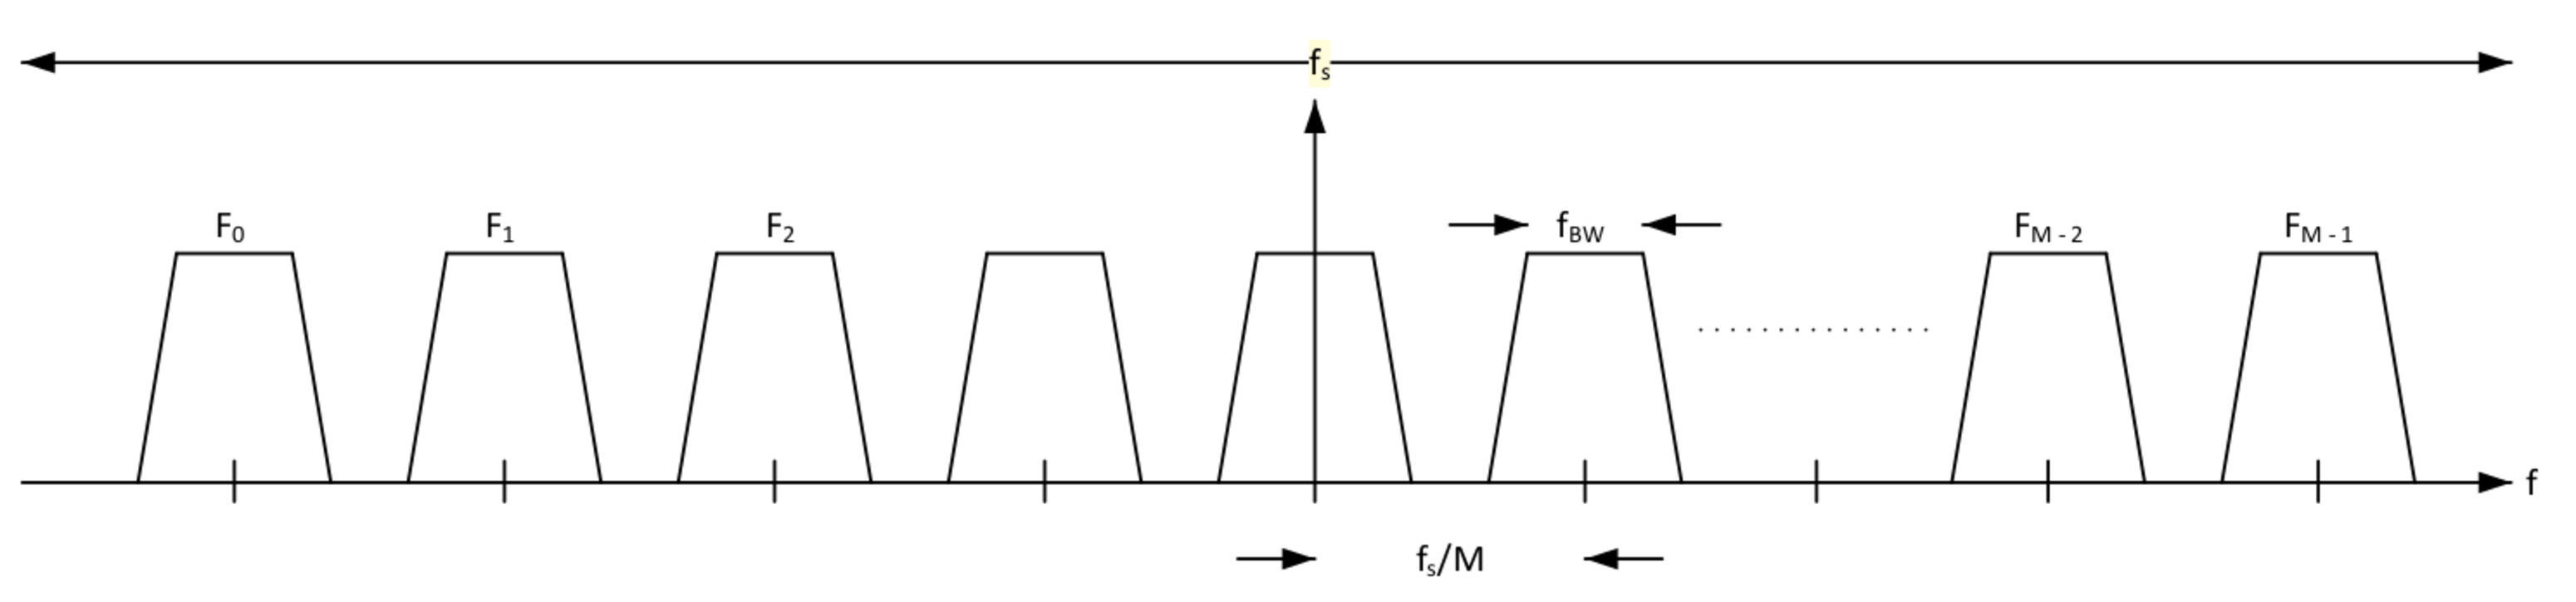
\includegraphics[width=0.8\textwidth]{FDM_channel_diagram}
				\end{center}
\end{frame}
\begin{frame}{Canalizador}
				\framesubtitle{Operación básica}
				\centering
								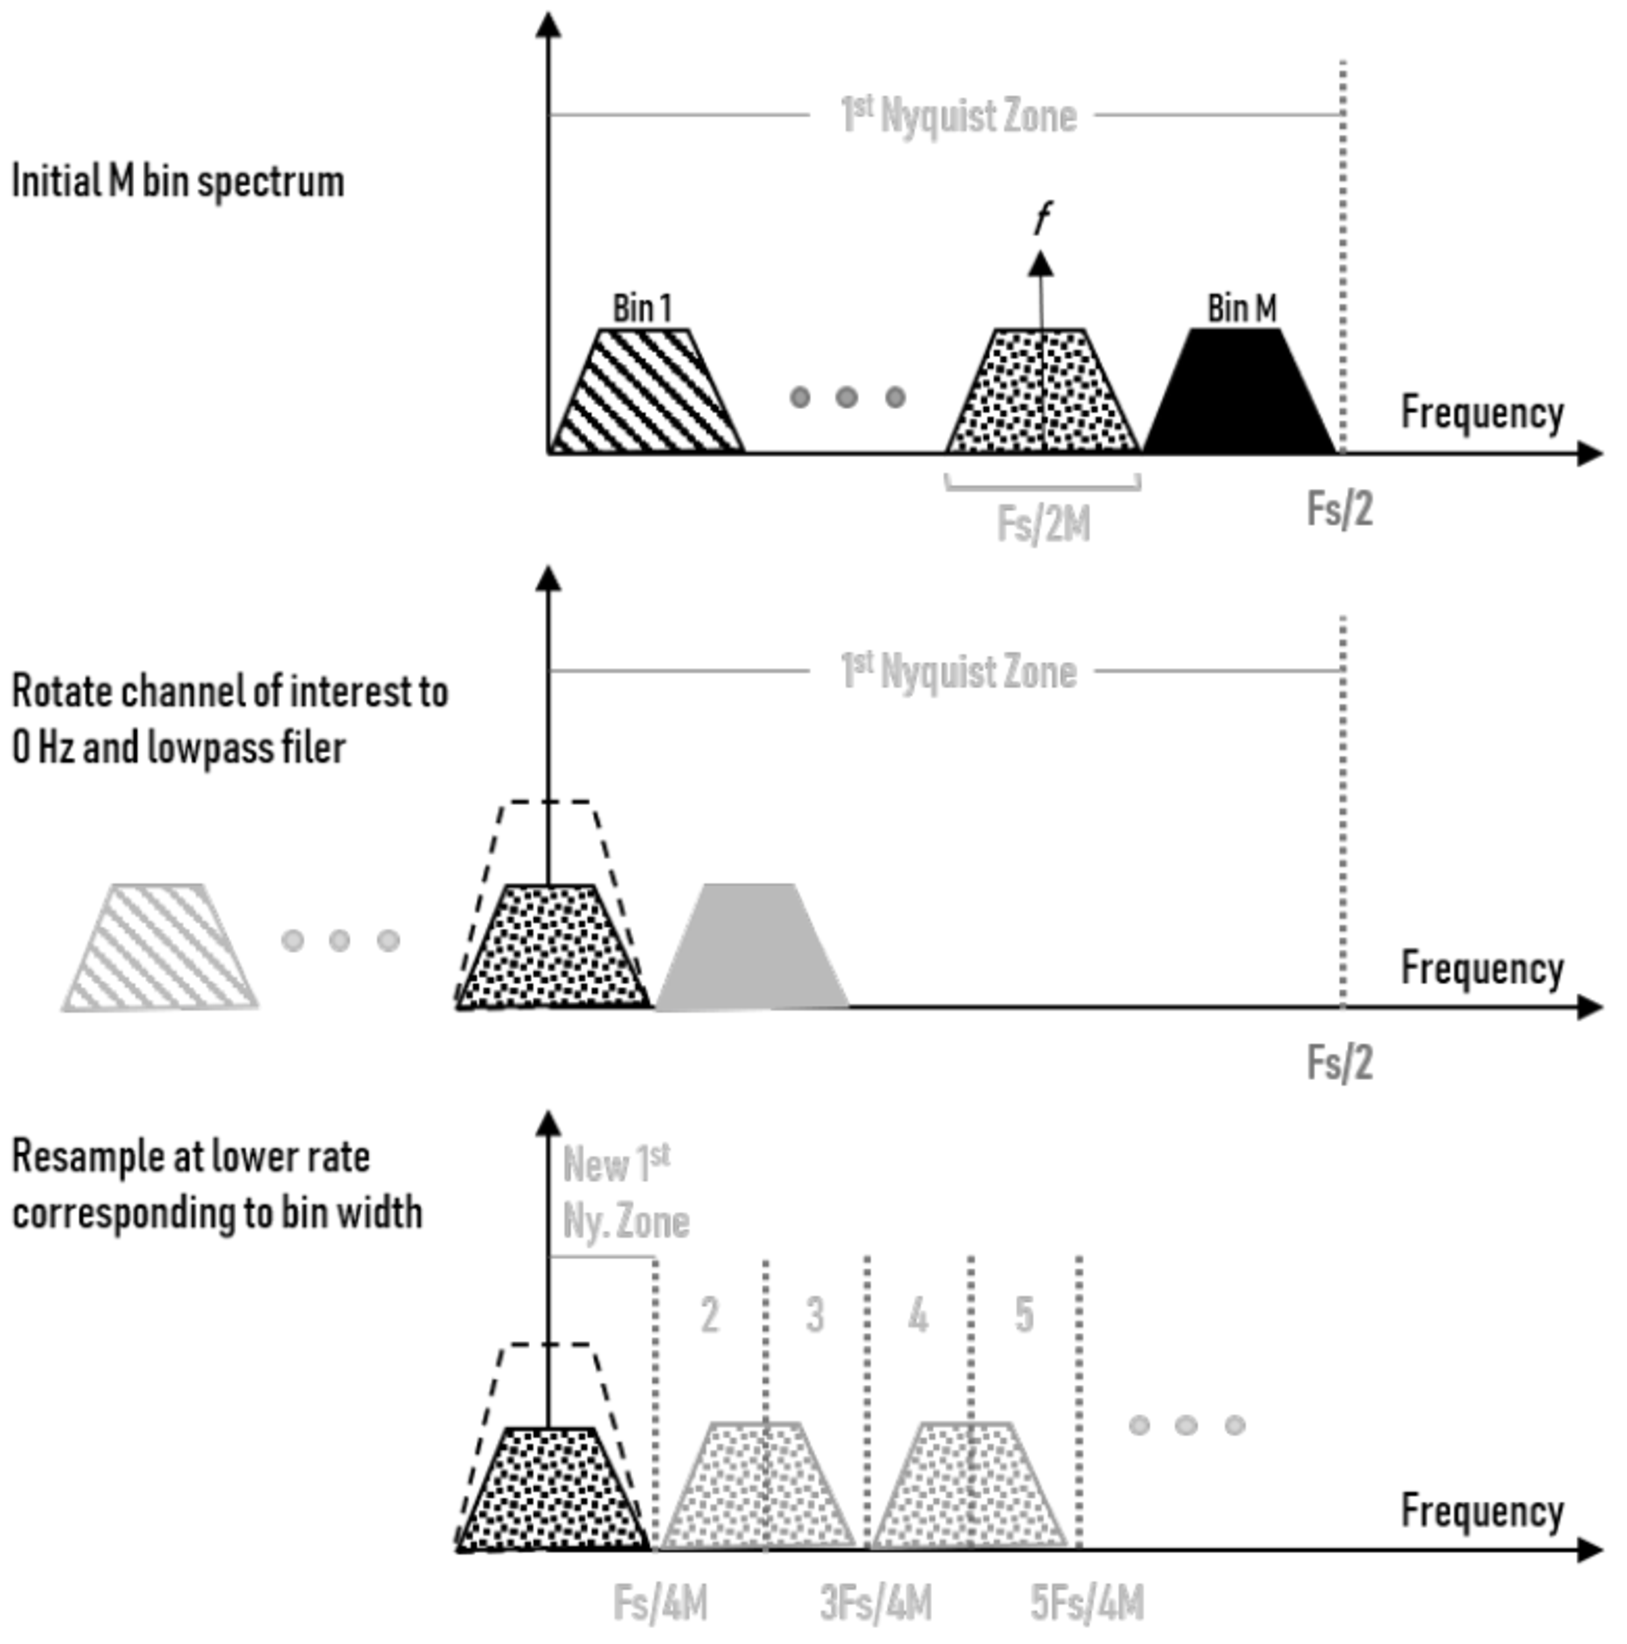
\includegraphics[width=0.7\textwidth]{pfb_basic1}
\end{frame}
\begin{frame}{Canalizador}
				\framesubtitle{Operación básica}
				\begin{columns}
								\begin{column}{0.5\textwidth}
												\begin{itemize}
																\item Basado en el concepto de filtro polifásico
																				\begin{equation*}\label{eq_transformada_z}
																								X(z) = \sum_{n = -\infty}^{\infty}x(n)\,z^{-n}
																				\end{equation*}


												\end{itemize}
								\end{column}
								\begin{column}{0.5\textwidth}
				\centering
								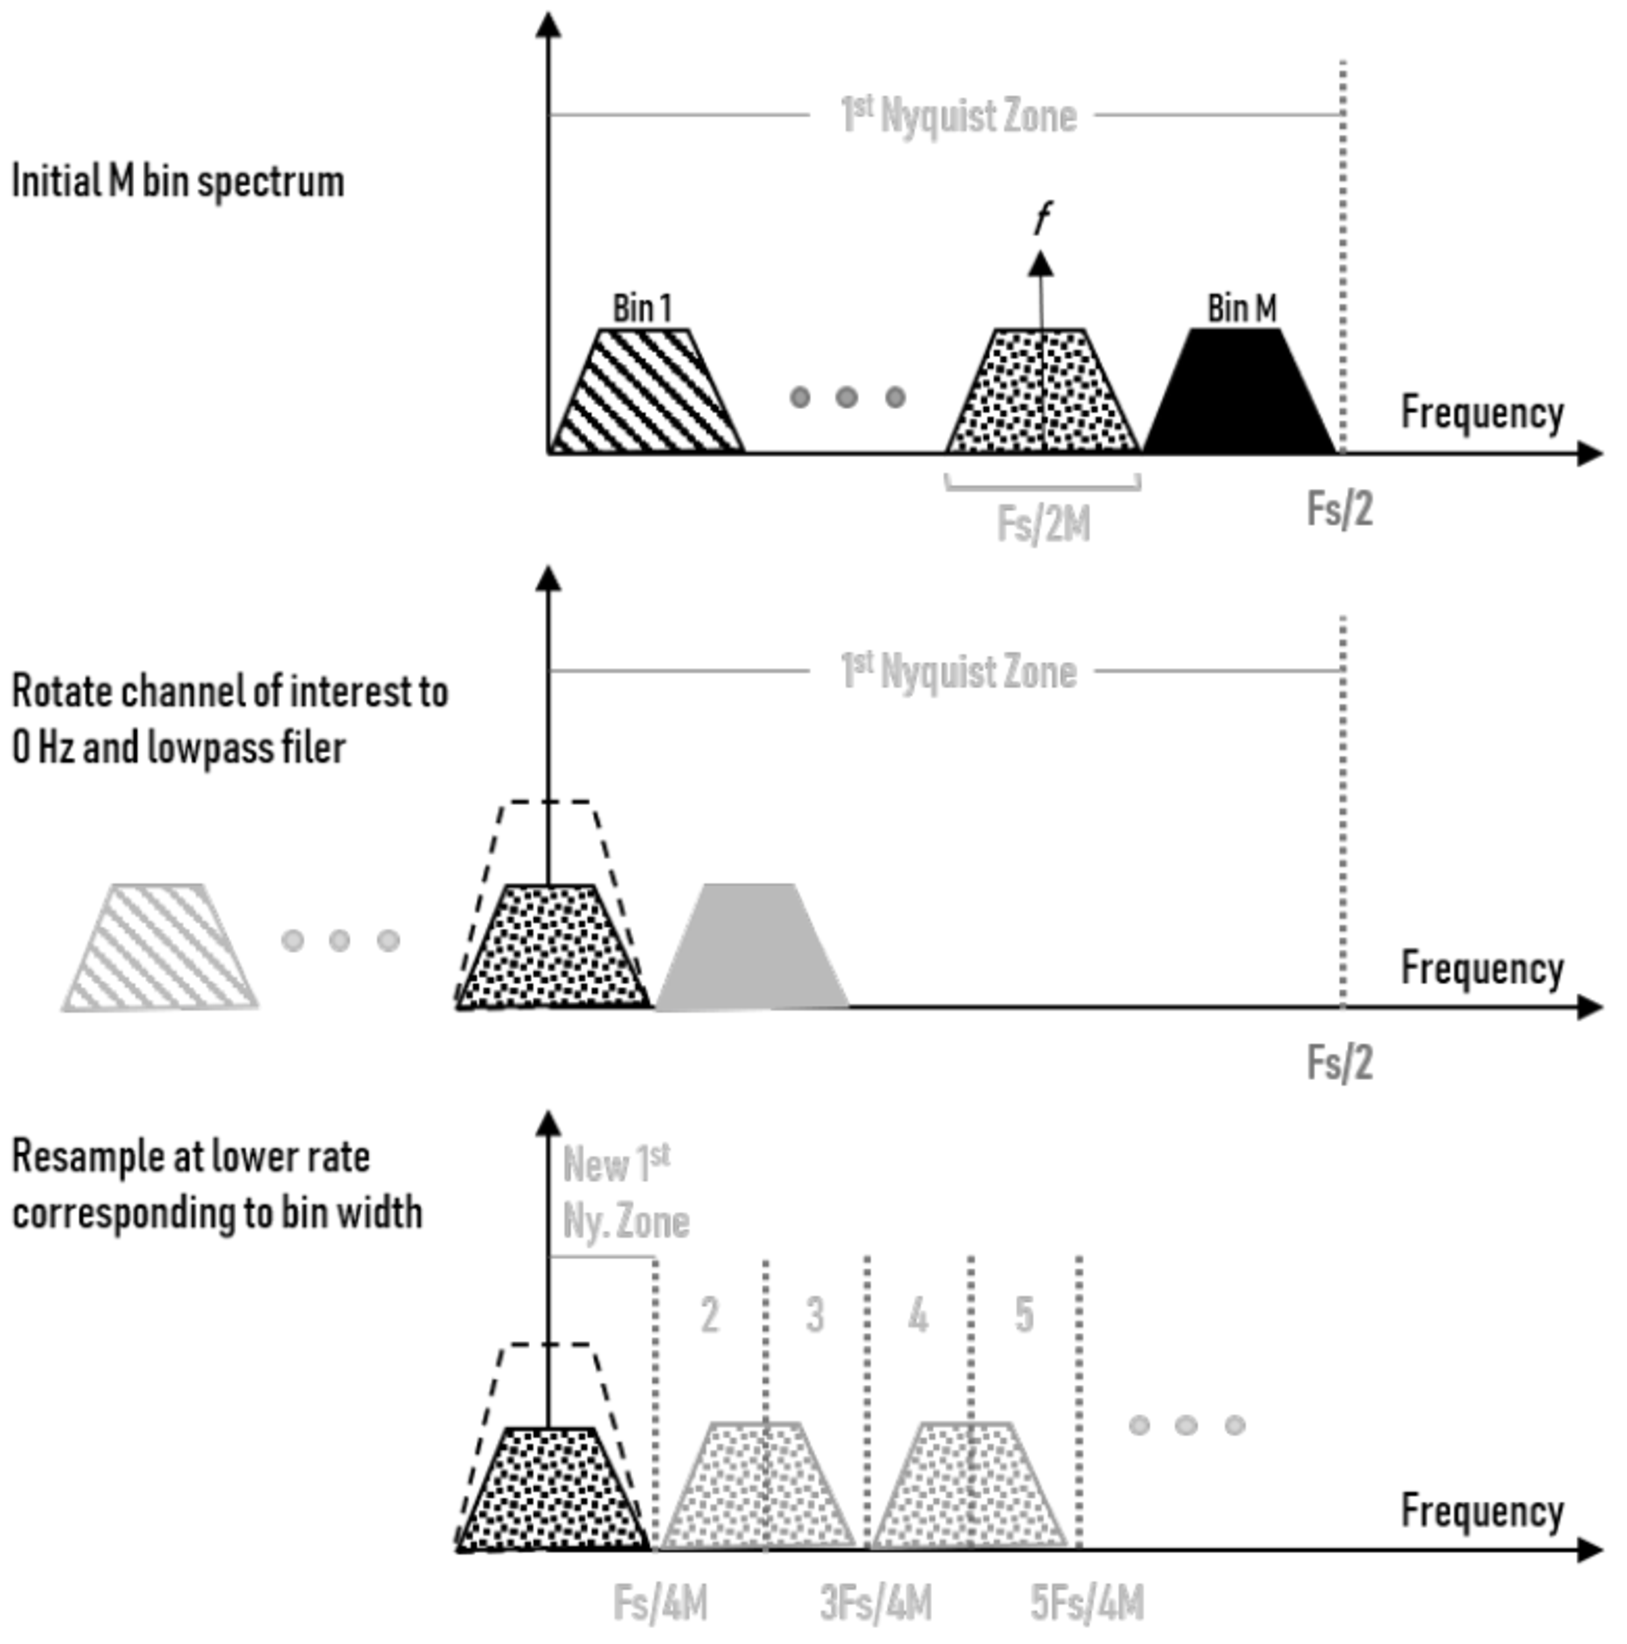
\includegraphics[width=0.7\textwidth]{pfb_basic1}
								\end{column}
								\end{columns}
																				\begin{equation*}\label{eq_transformada_z_polifasica}
																								X(z) = \sum_{\lambda =
																								0}^{M-1}z^{-\lambda}\,X_\lambda^{(p)}(z^{M})
																				\end{equation*}
																				{\color{blue}\begin{equation*}\label{eq_x_polifasica}
																								X_\lambda^{(p)}(z^{M}) = \sum_{m =-\infty}^{\infty}x(mM+\lambda)\,z^{-mM}
																				\end{equation*}}


\end{frame}
\begin{frame}{Canalizador}
				\framesubtitle{Operación básica}
				\begin{center}
								\only<1>{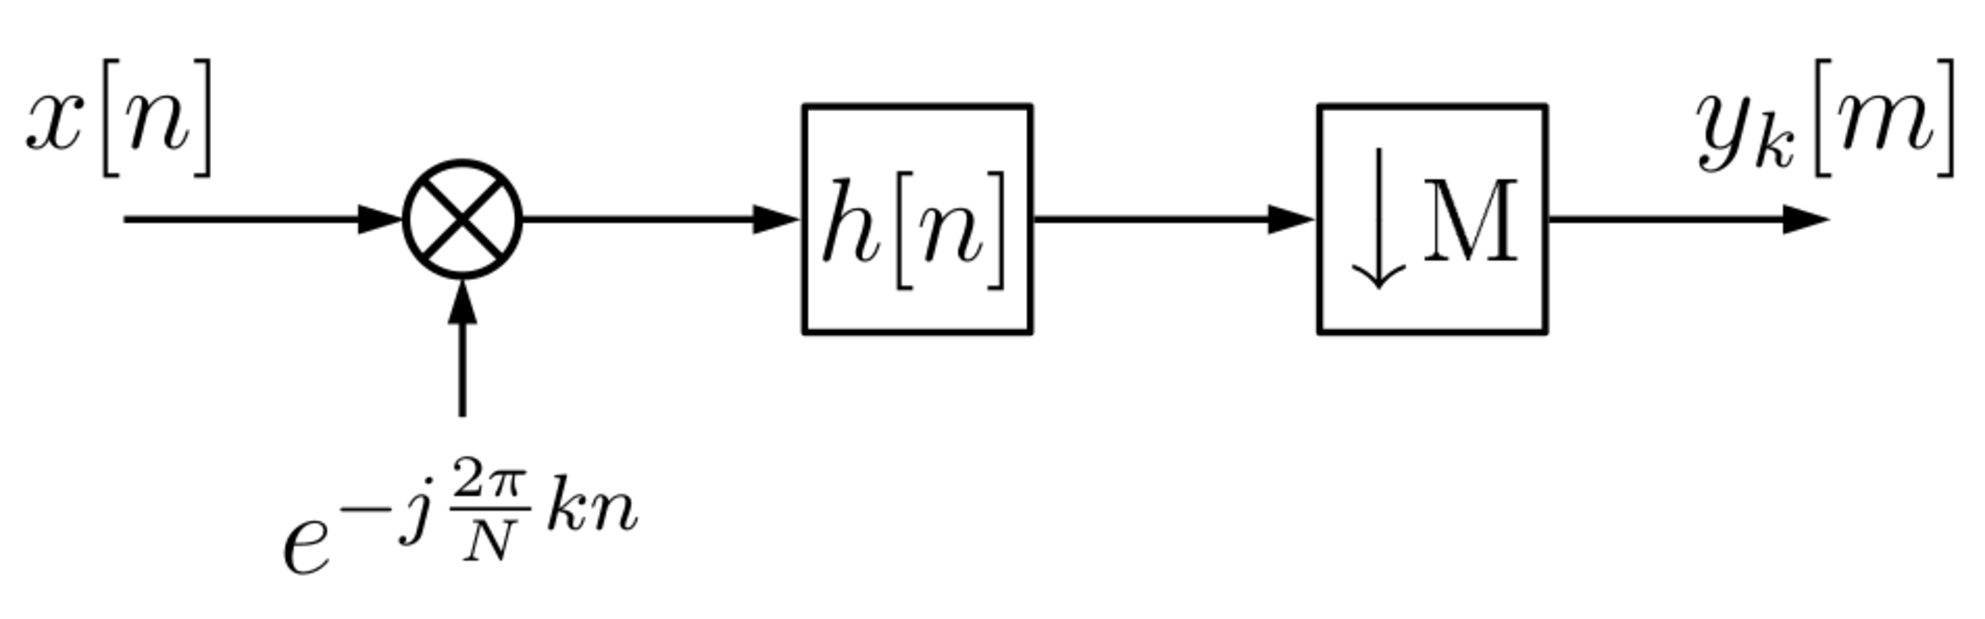
\includegraphics[width=0.8\textwidth]{PFB_basic_operation}}
				\end{center}
								\begin{center}
												\only<2>{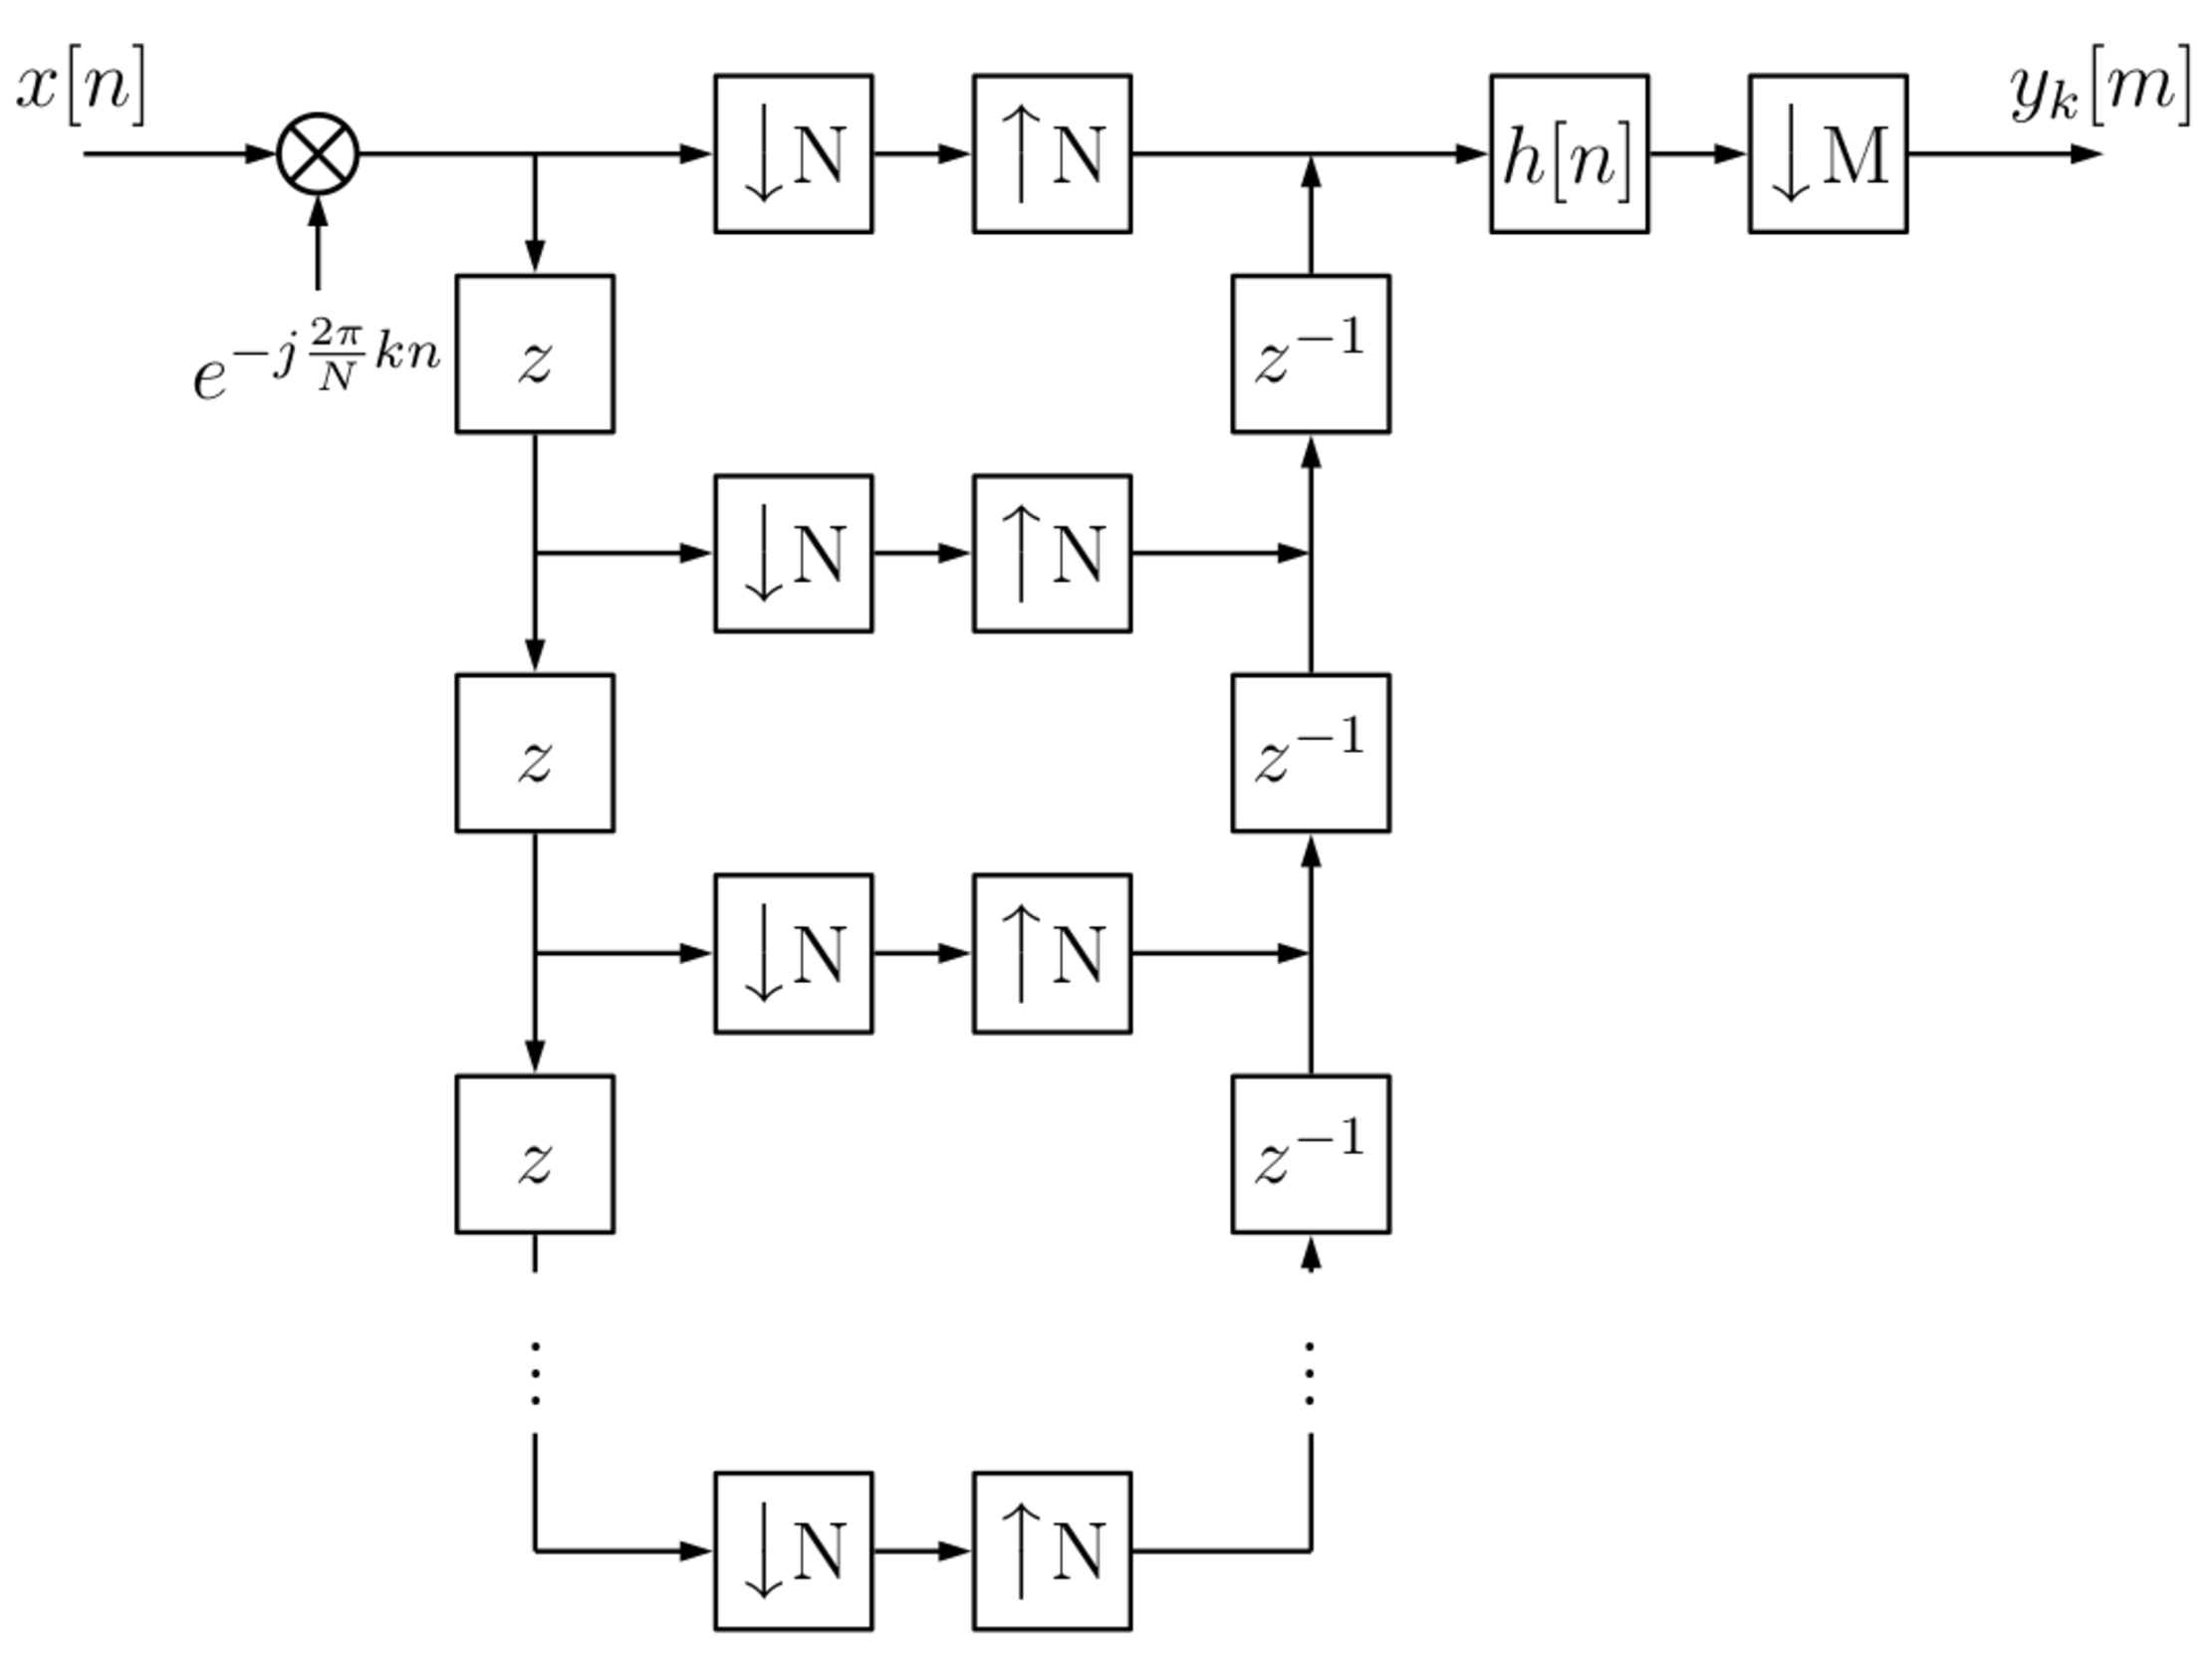
\includegraphics[width=0.5\textwidth]{PFB_opening_after_modulation}}
								\end{center}
\end{frame}
\begin{frame}{Channelizer operación básica}
				\begin{center}
								\only<1>{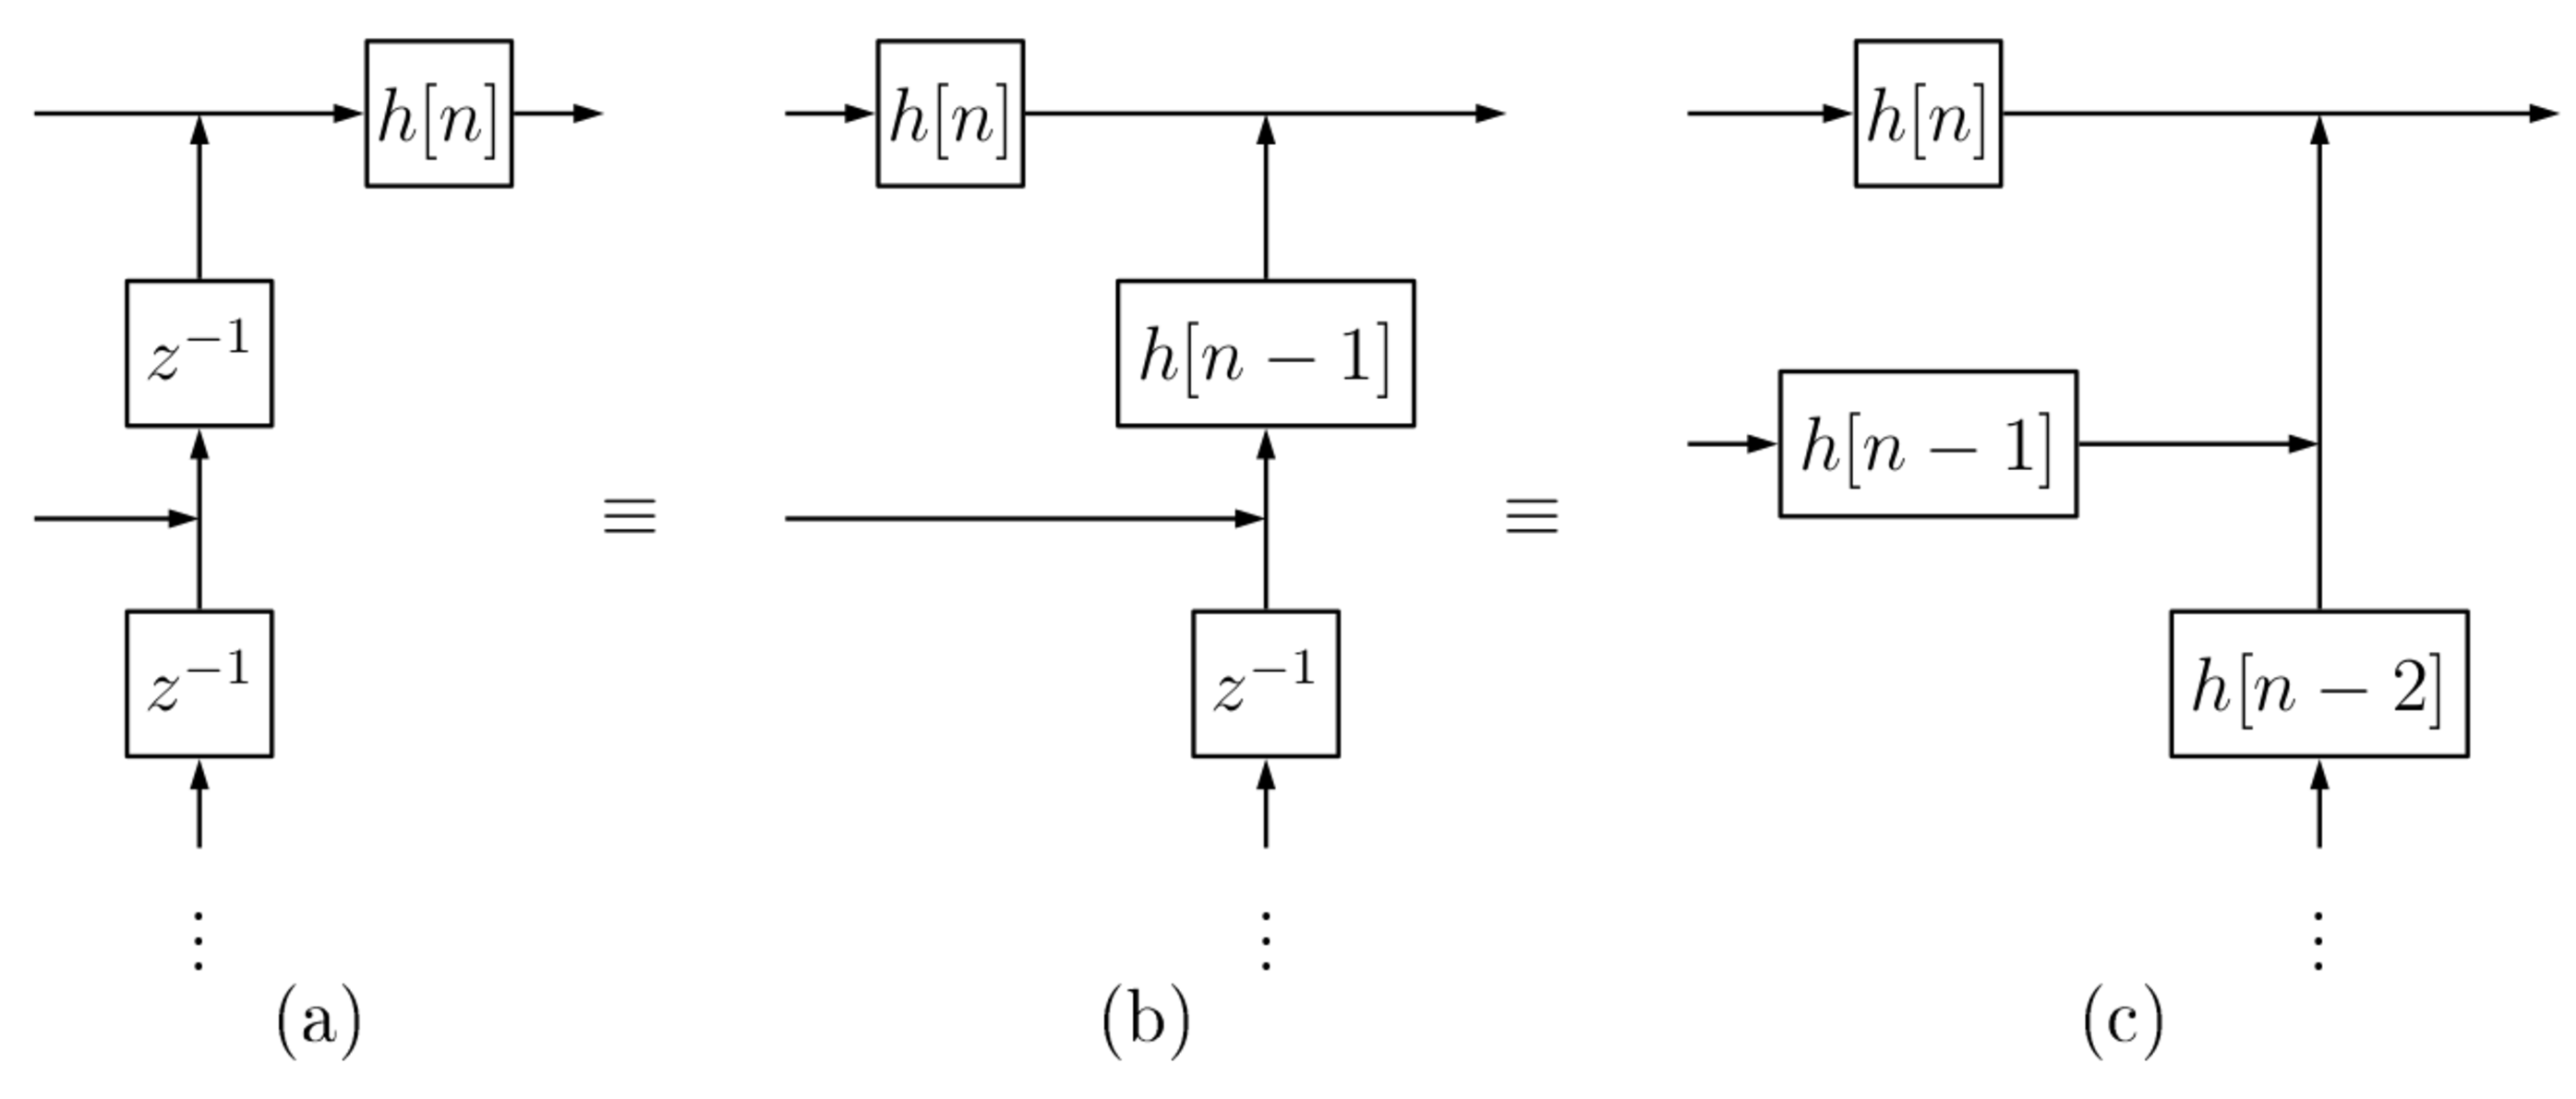
\includegraphics[width=0.8\textwidth]{PFB_distribution_filter_branches}}
				\end{center}
								\begin{center}
												\only<2>{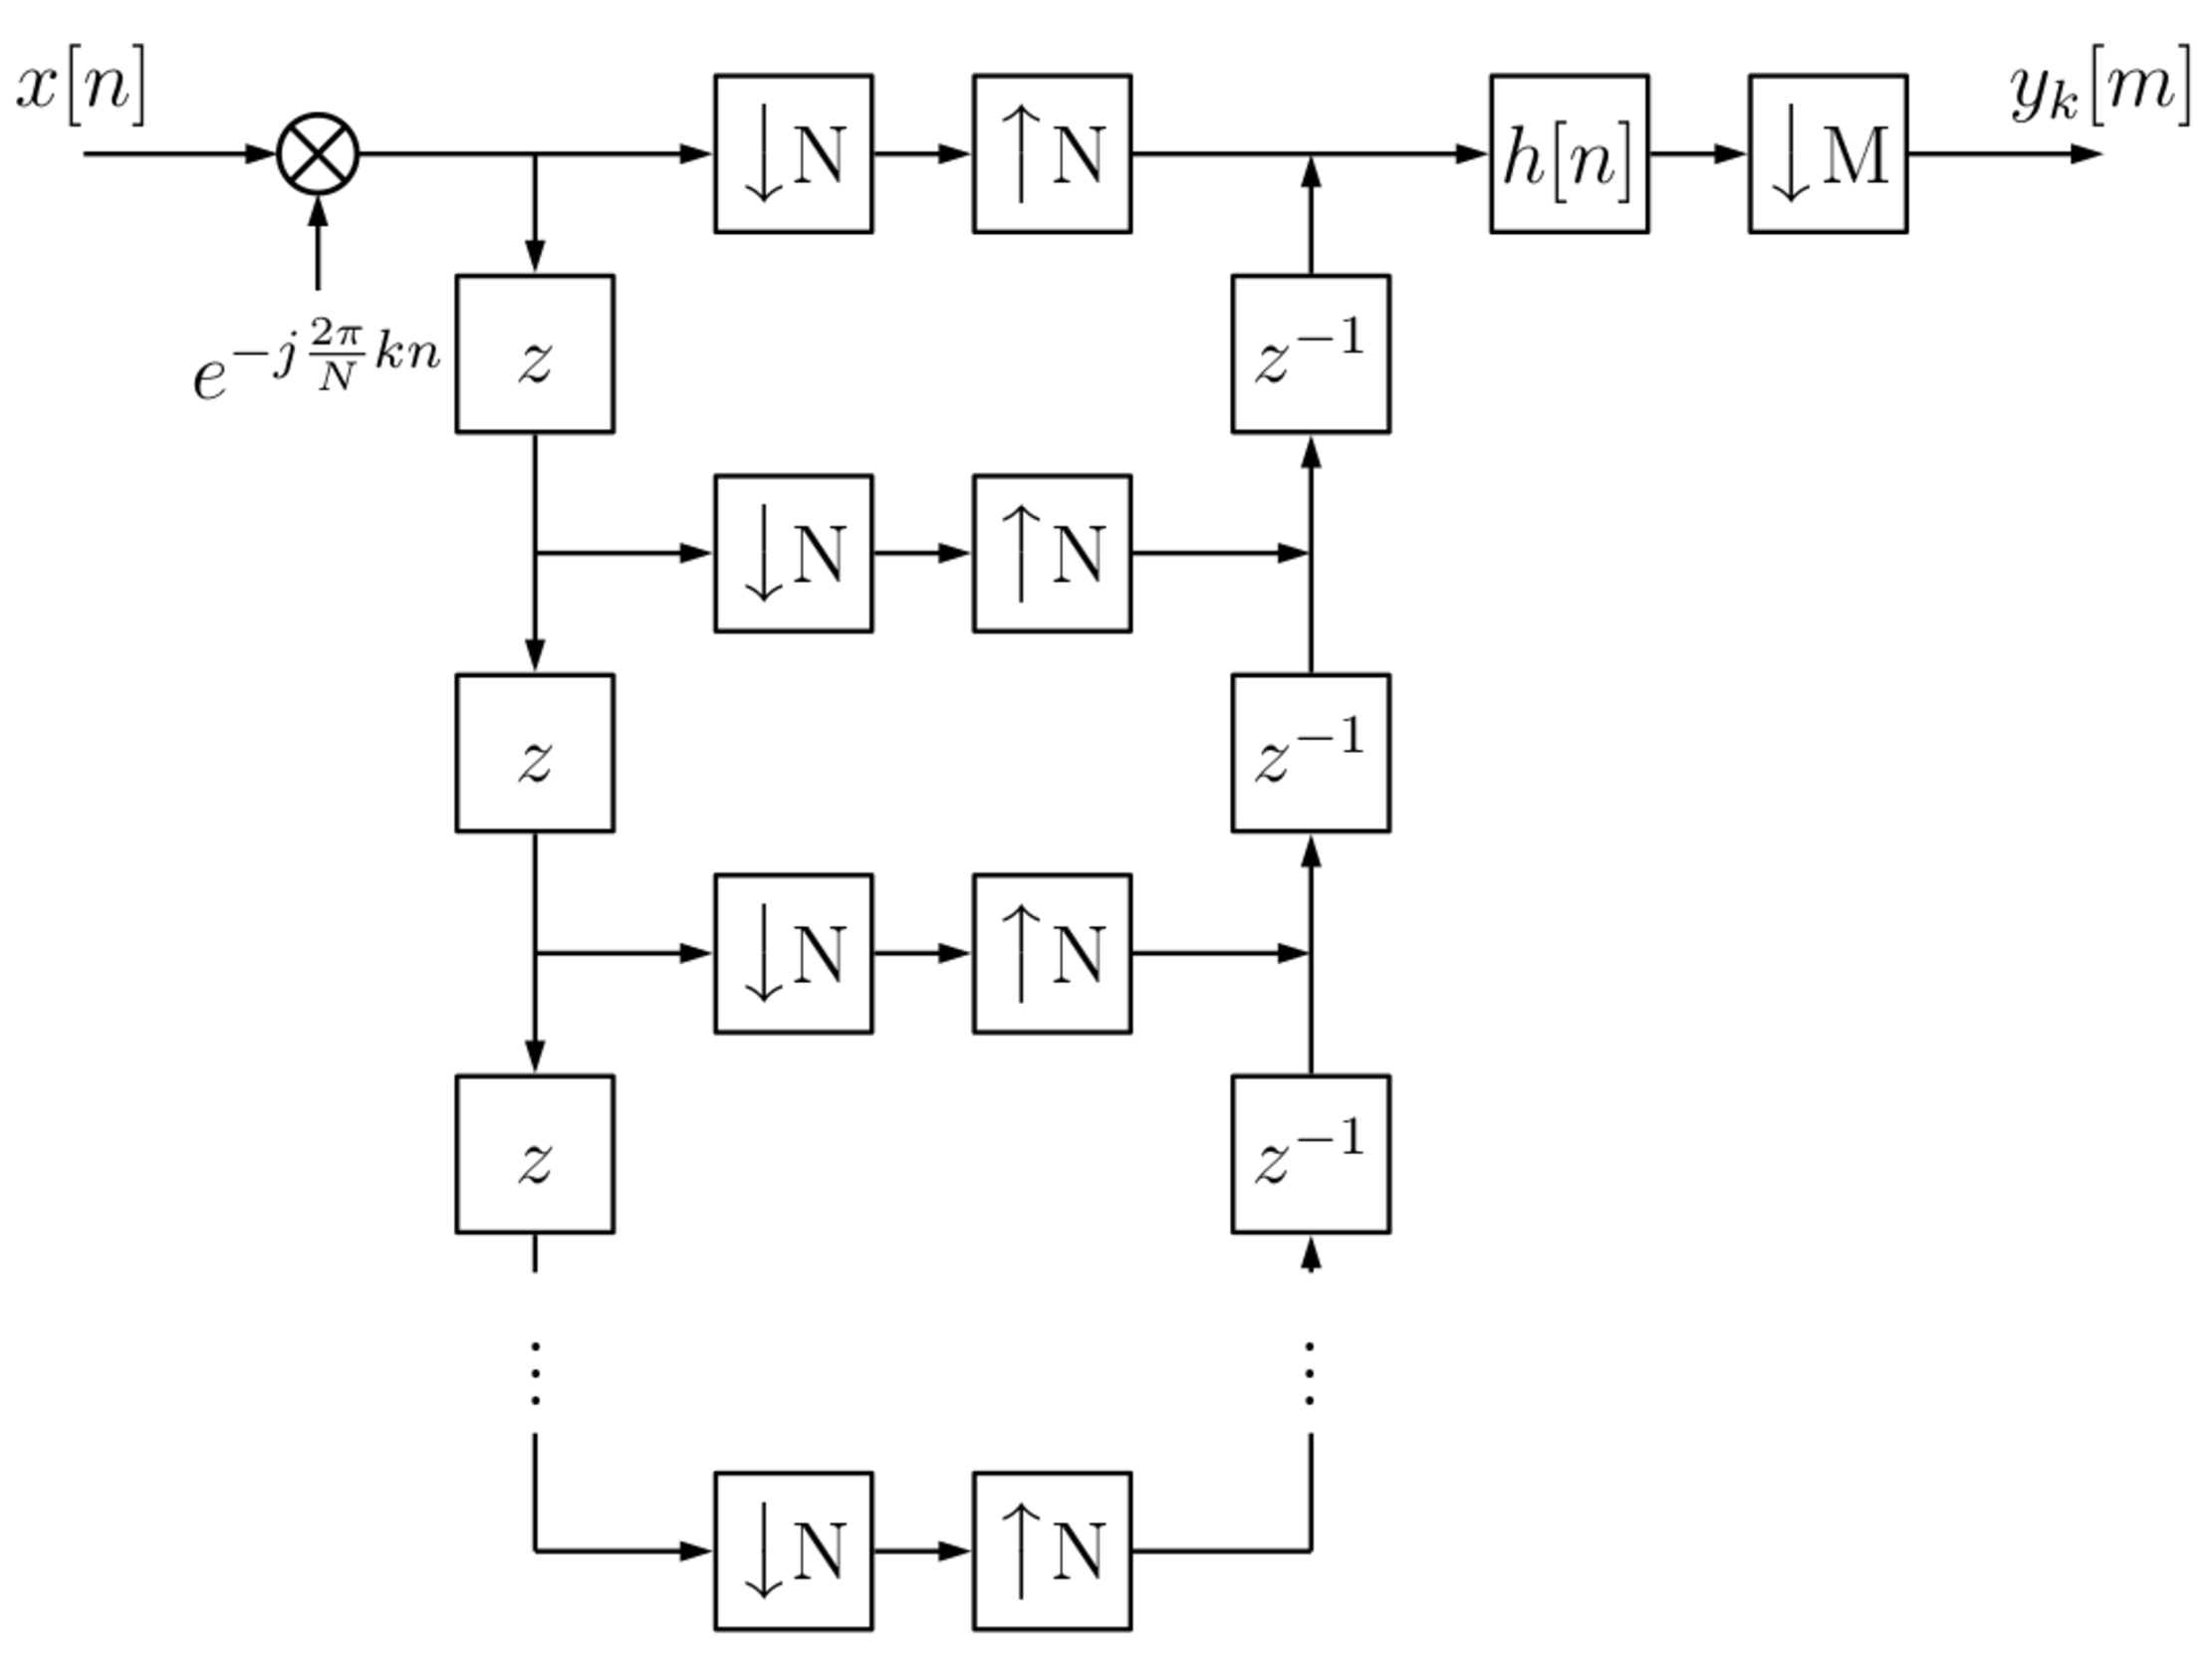
\includegraphics[width=0.8\textwidth]{PFB_opening_after_modulation}}
								\end{center}
\end{frame}

\begin{frame}{Channelizer operación básica}
				\begin{center}
								\only<1>{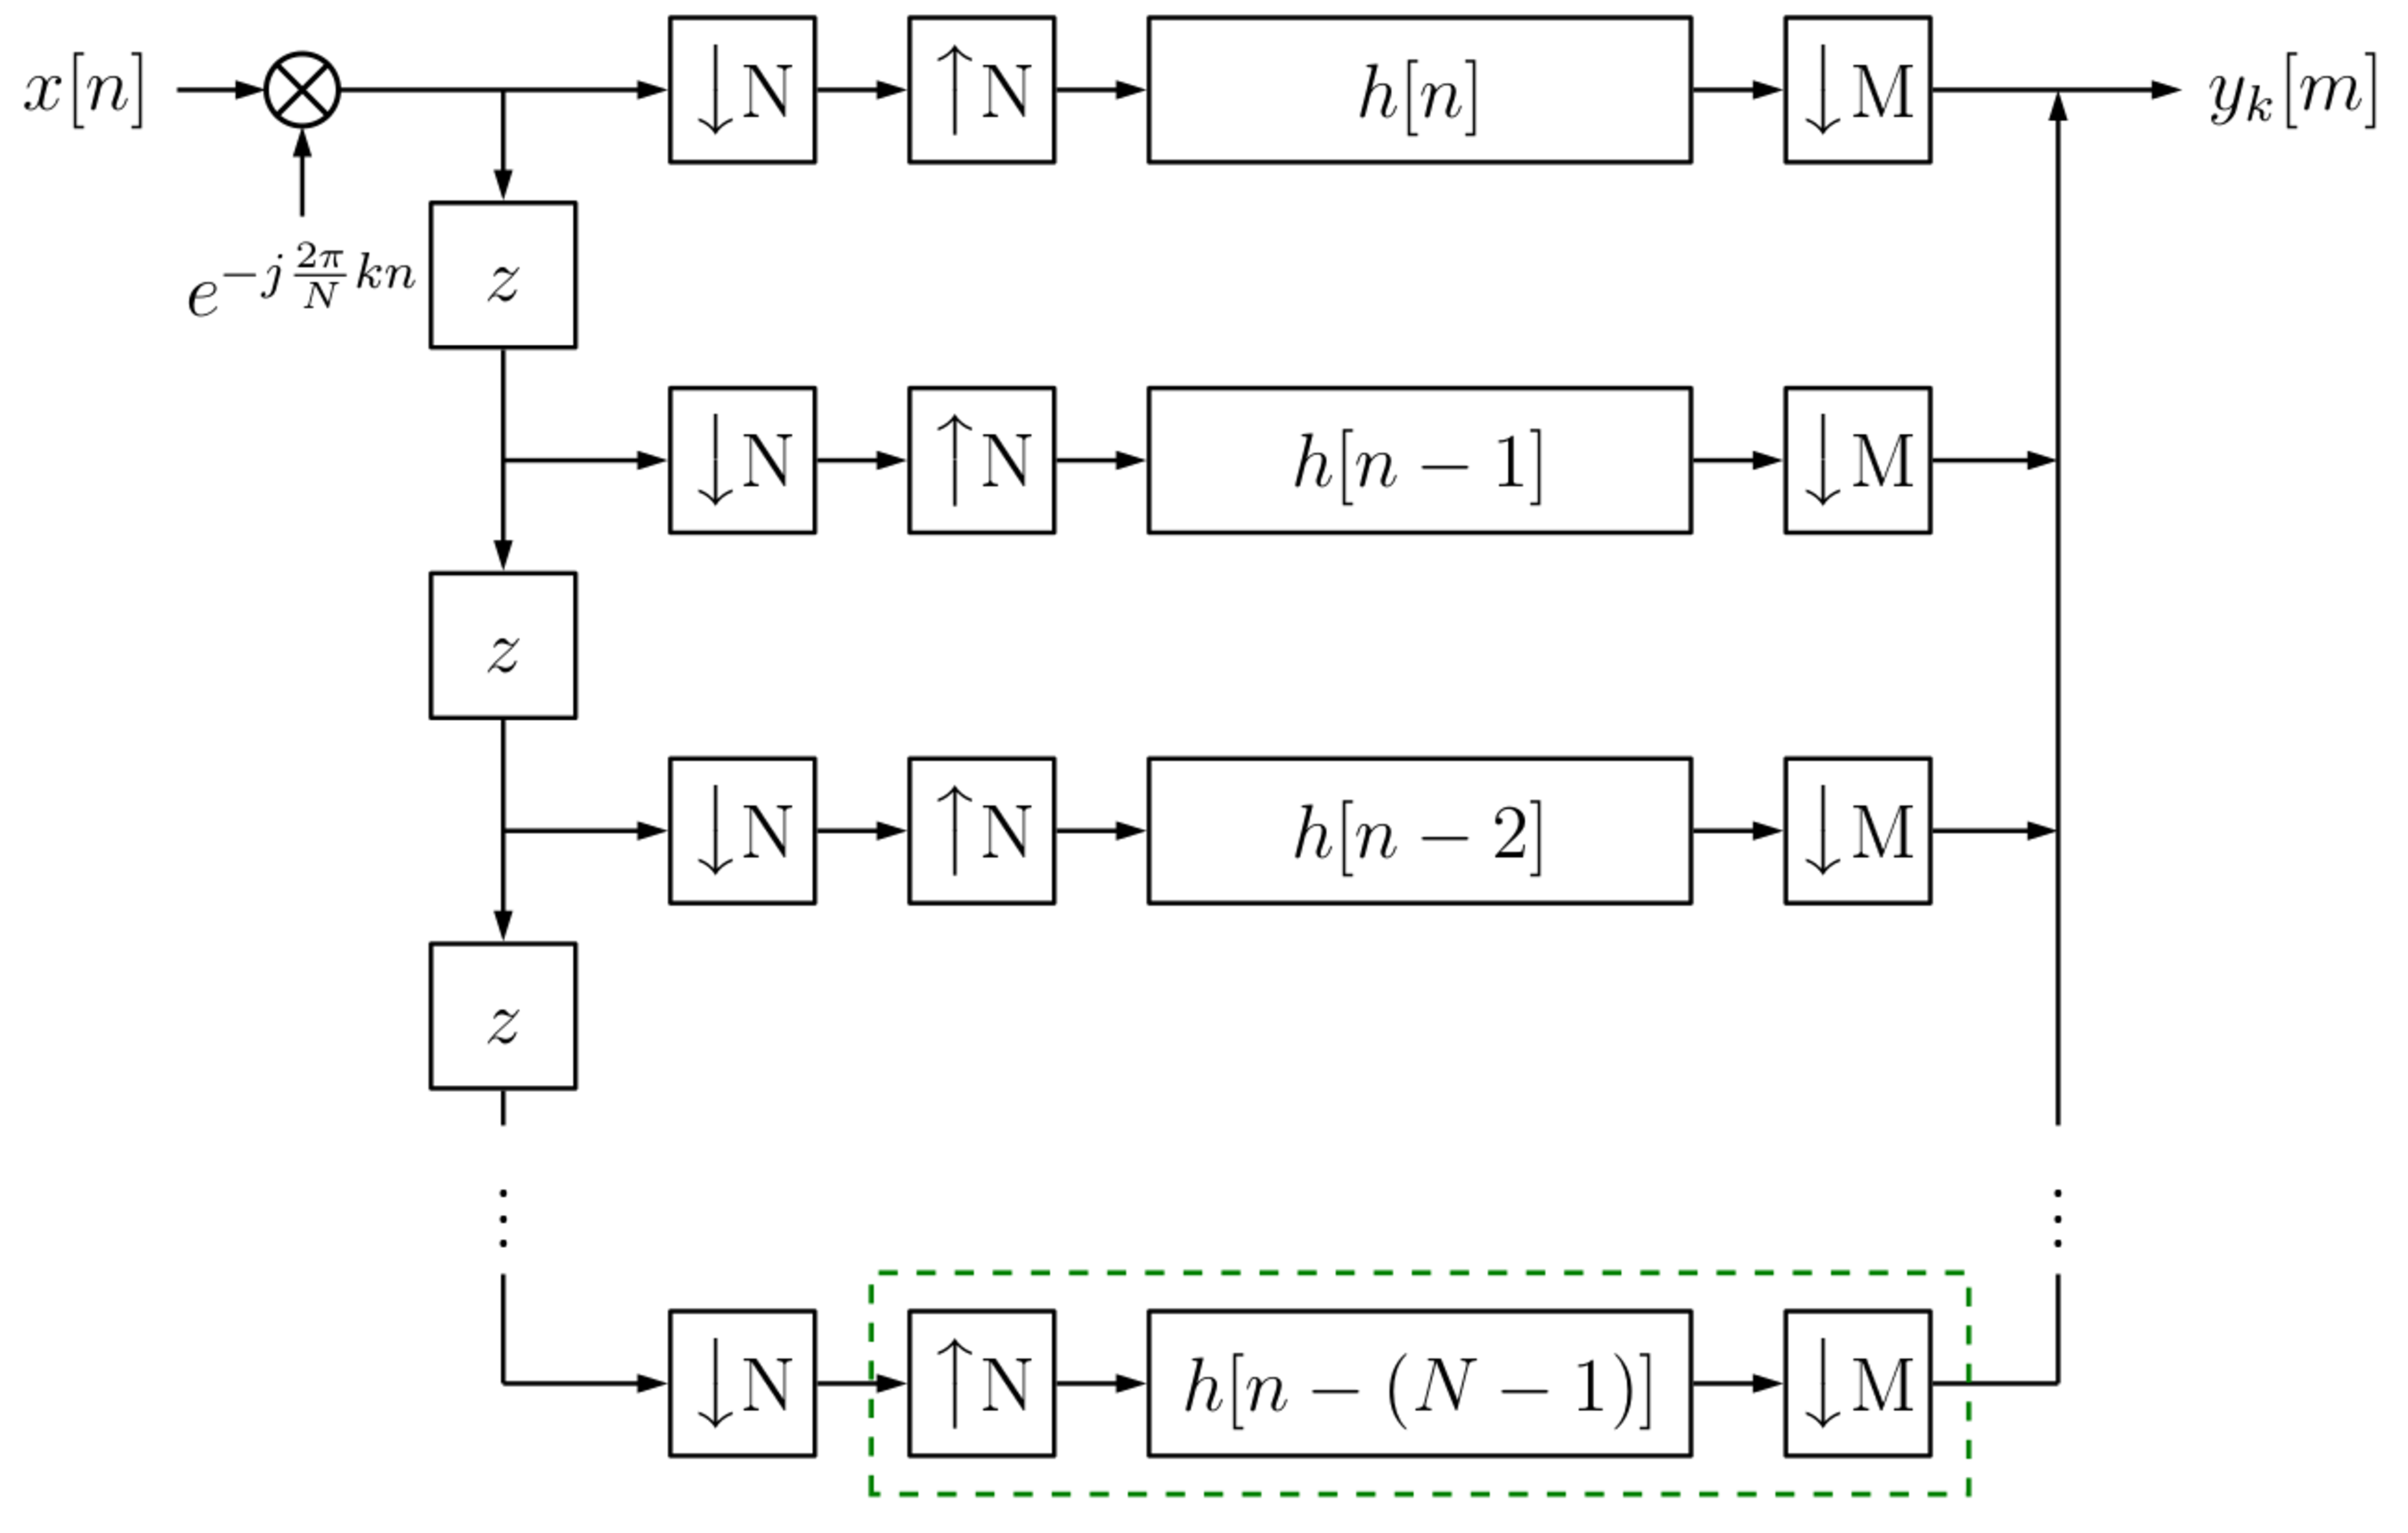
\includegraphics[width=0.8\textwidth]{PFB_distribution_filter_decimators}}
				\end{center}
								\begin{center}
												\only<2>{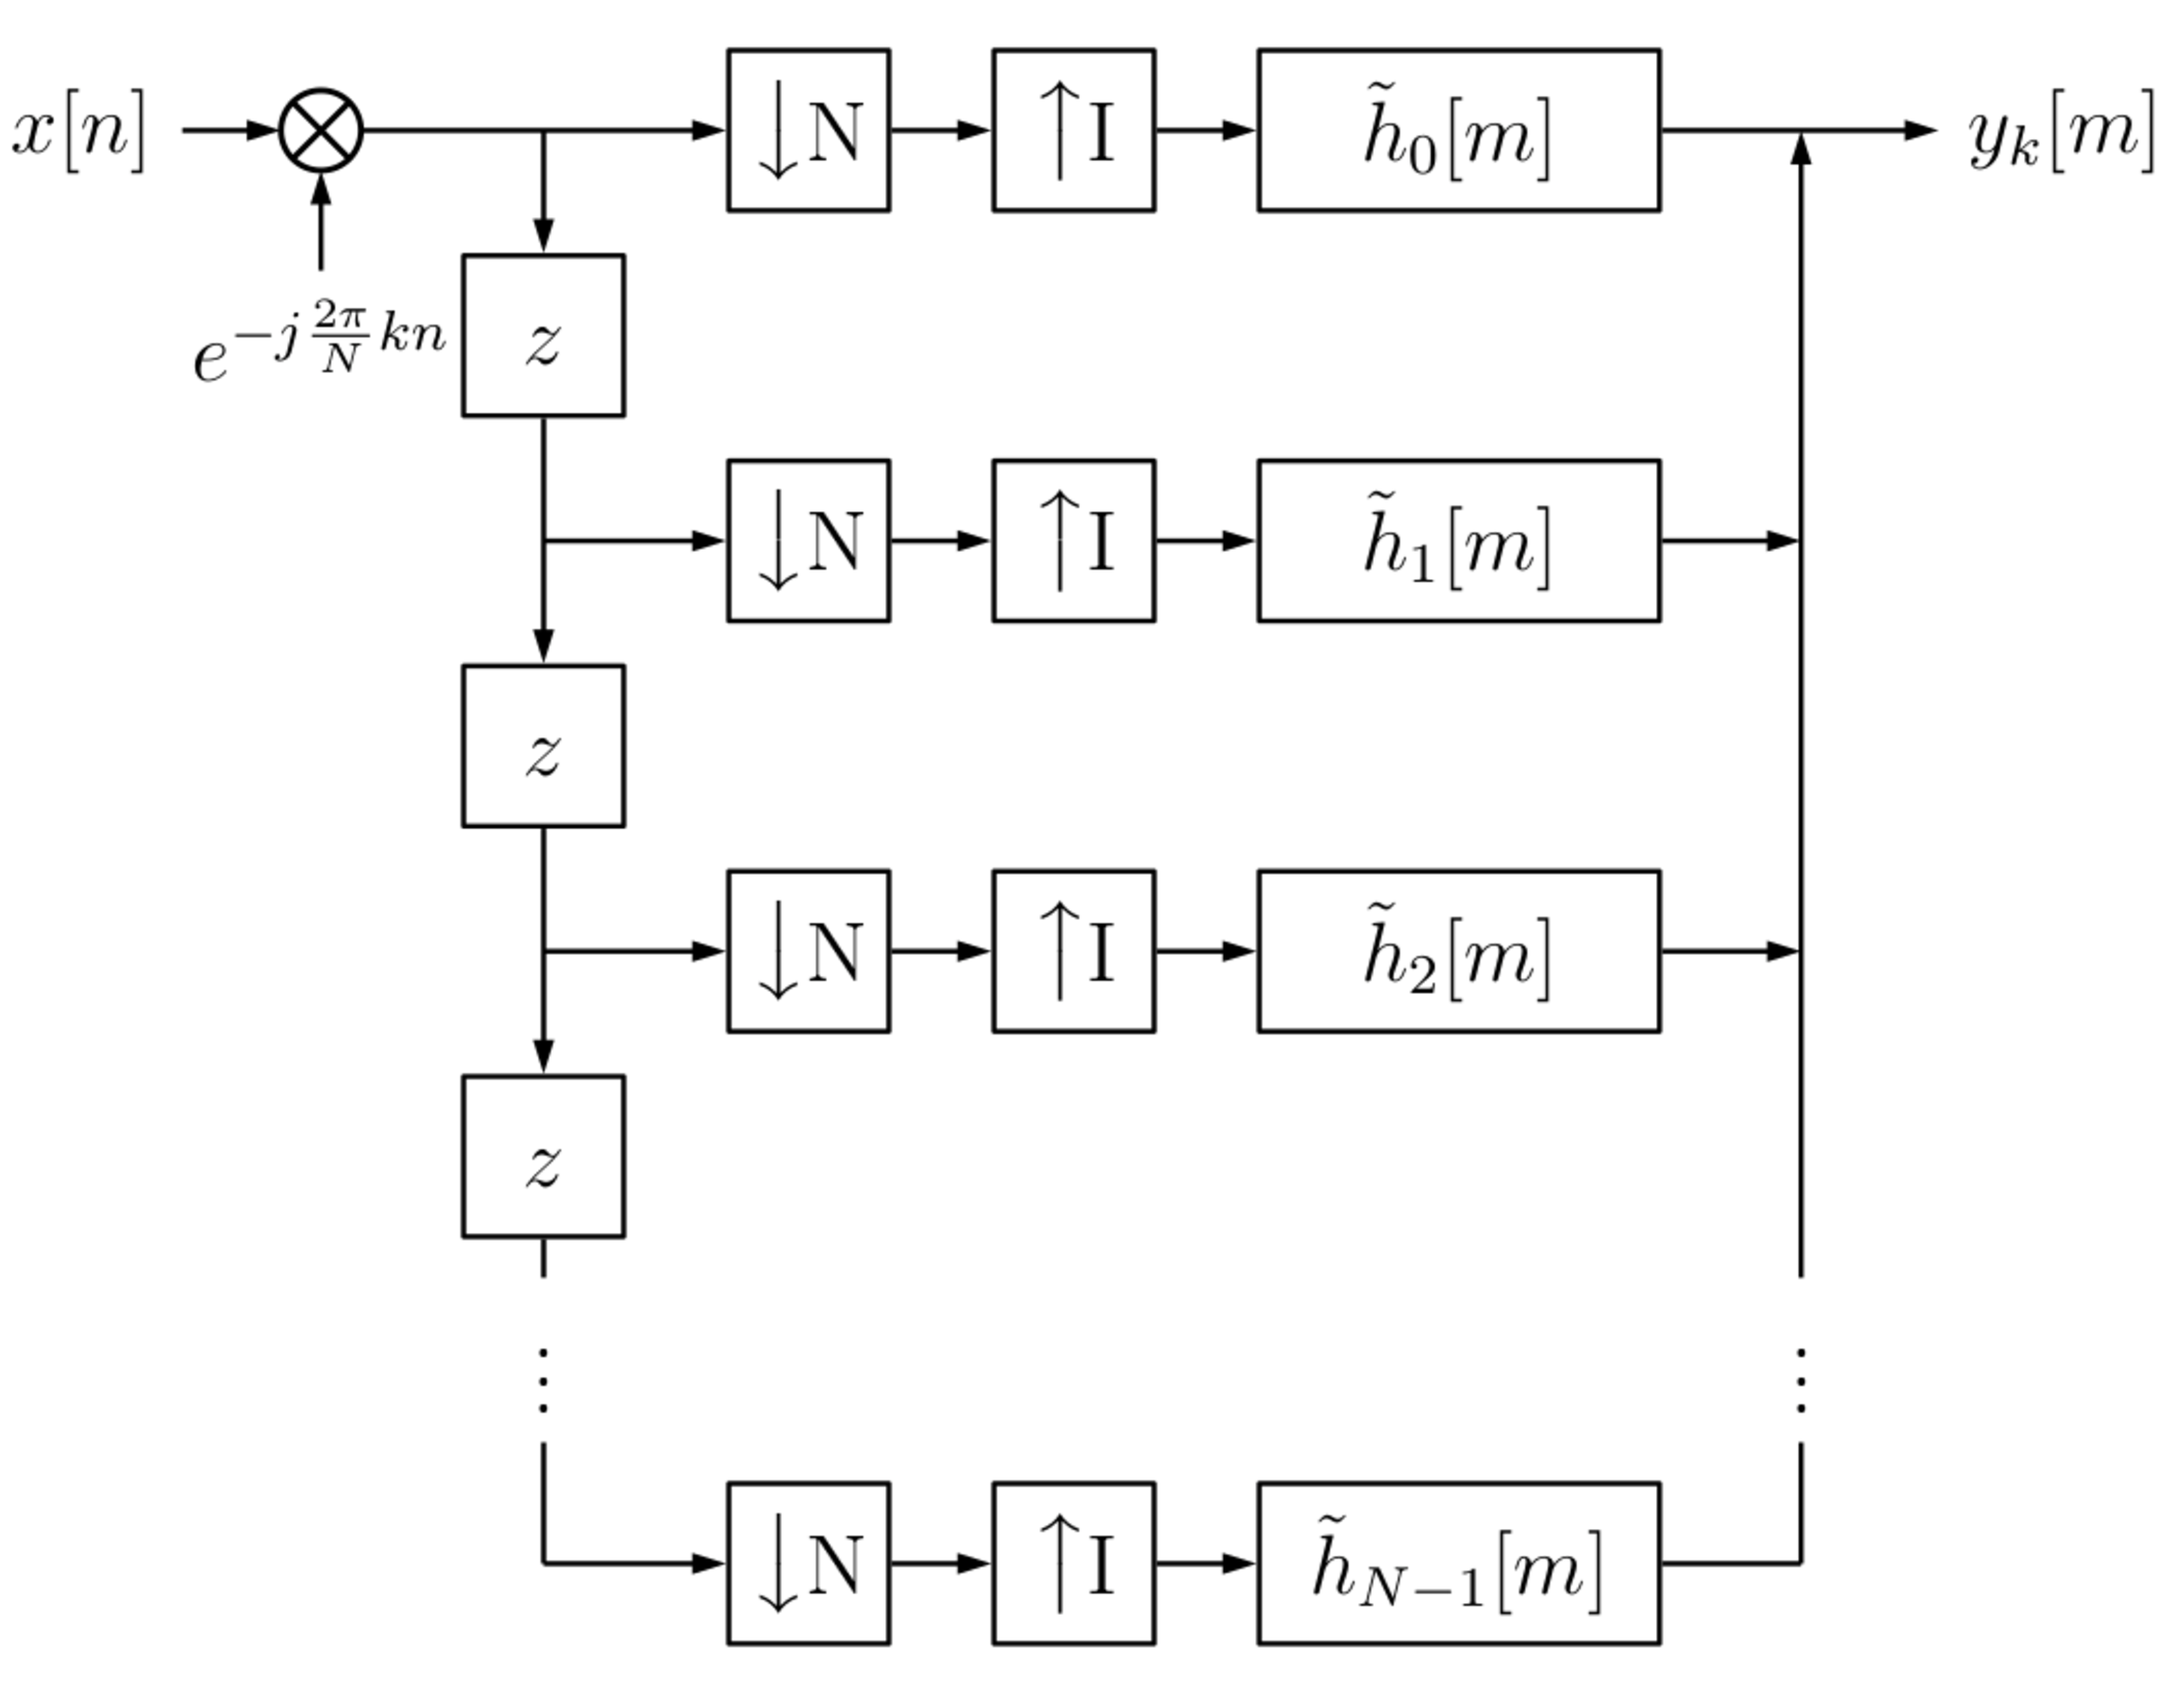
\includegraphics[width=0.8\textwidth]{PFB_distribution_filter_interpolators}}
								\end{center}
\end{frame}

\begin{frame}{Channelizer operación básica}
				\begin{center}
								\only<1>{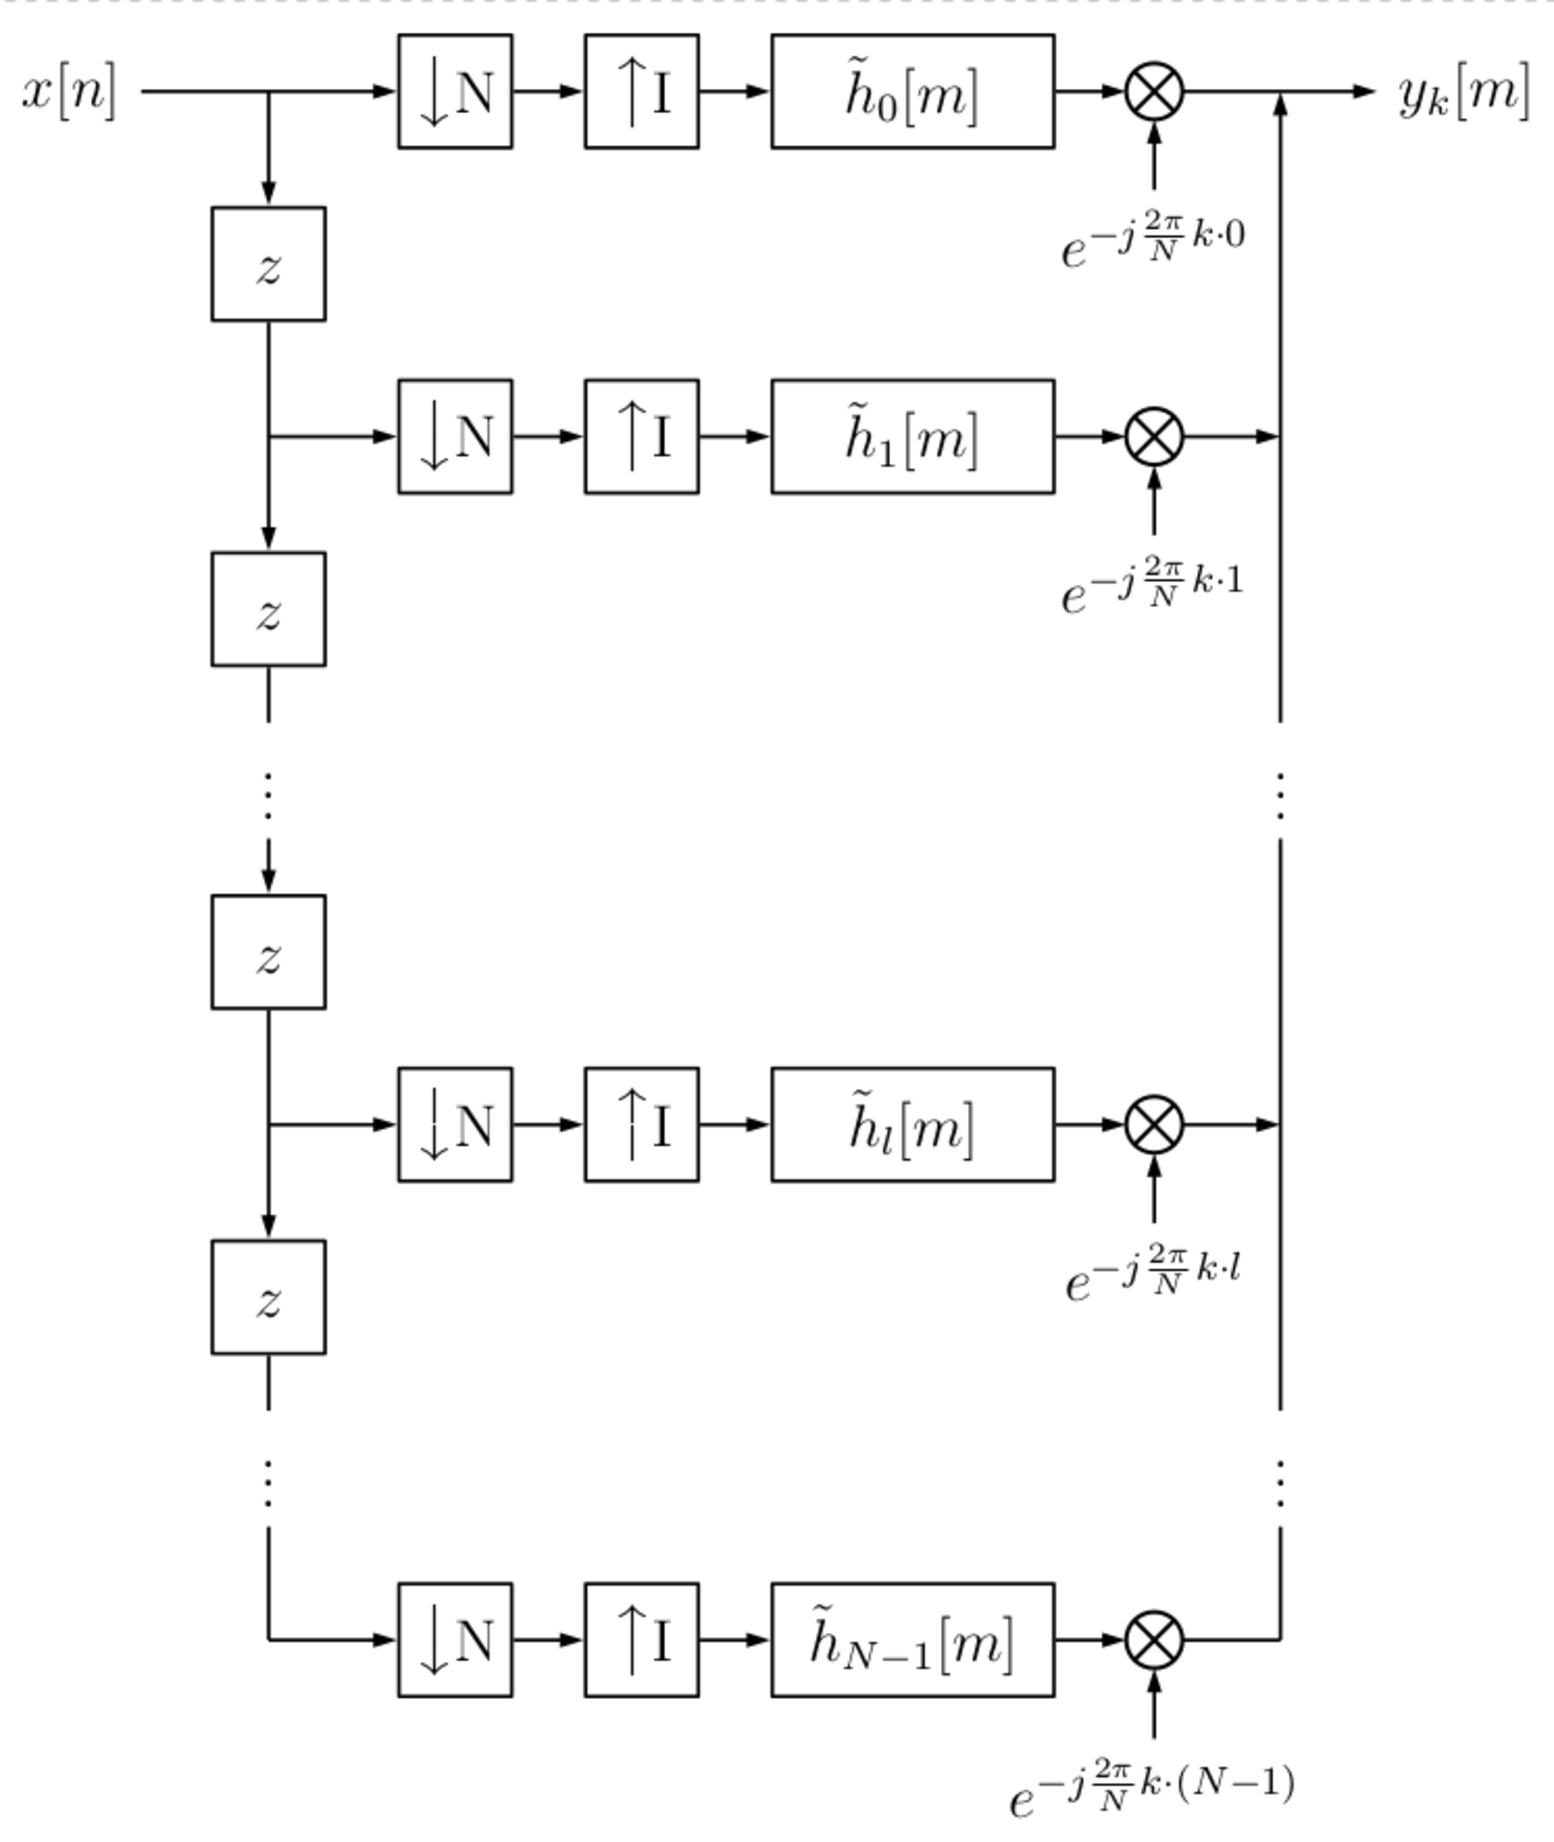
\includegraphics[width=0.6\textwidth]{PFB_distribution_modulators}}
				\end{center}
								\begin{center}
												\only<2>{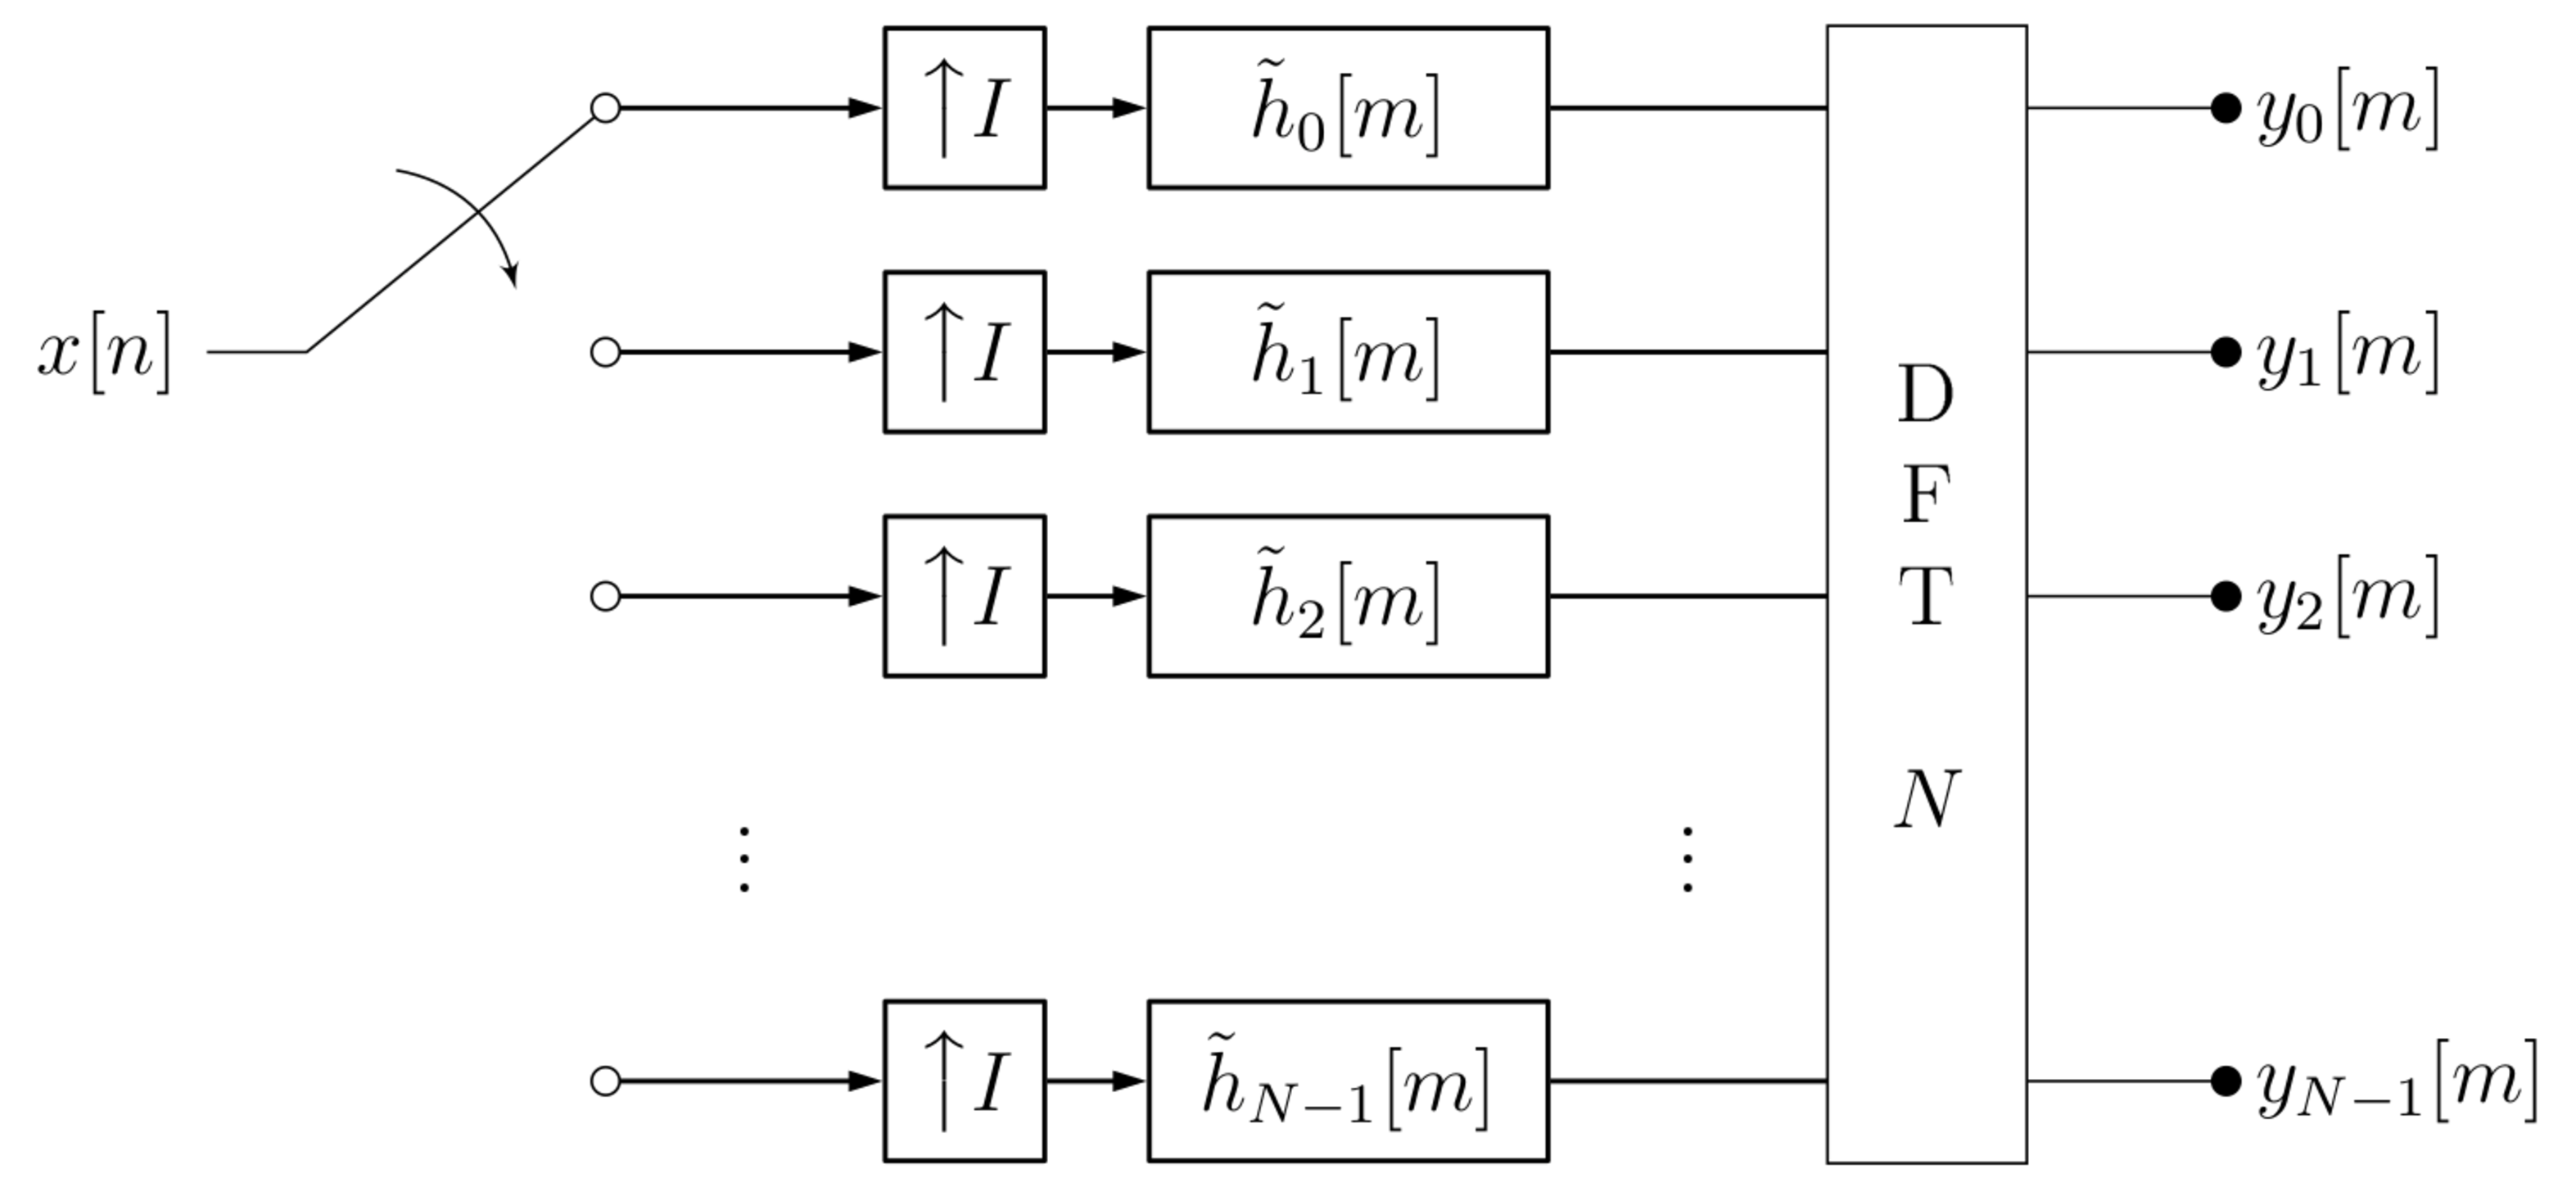
\includegraphics[width=0.8\textwidth]{PFB_final_arquitecture}}
								\end{center}
\end{frame}

\begin{frame}{Channelizer Tx}
				%\begin{columns}
				%				\begin{column}{0.65\textwidth}
				\begin{center}
								\only<1>{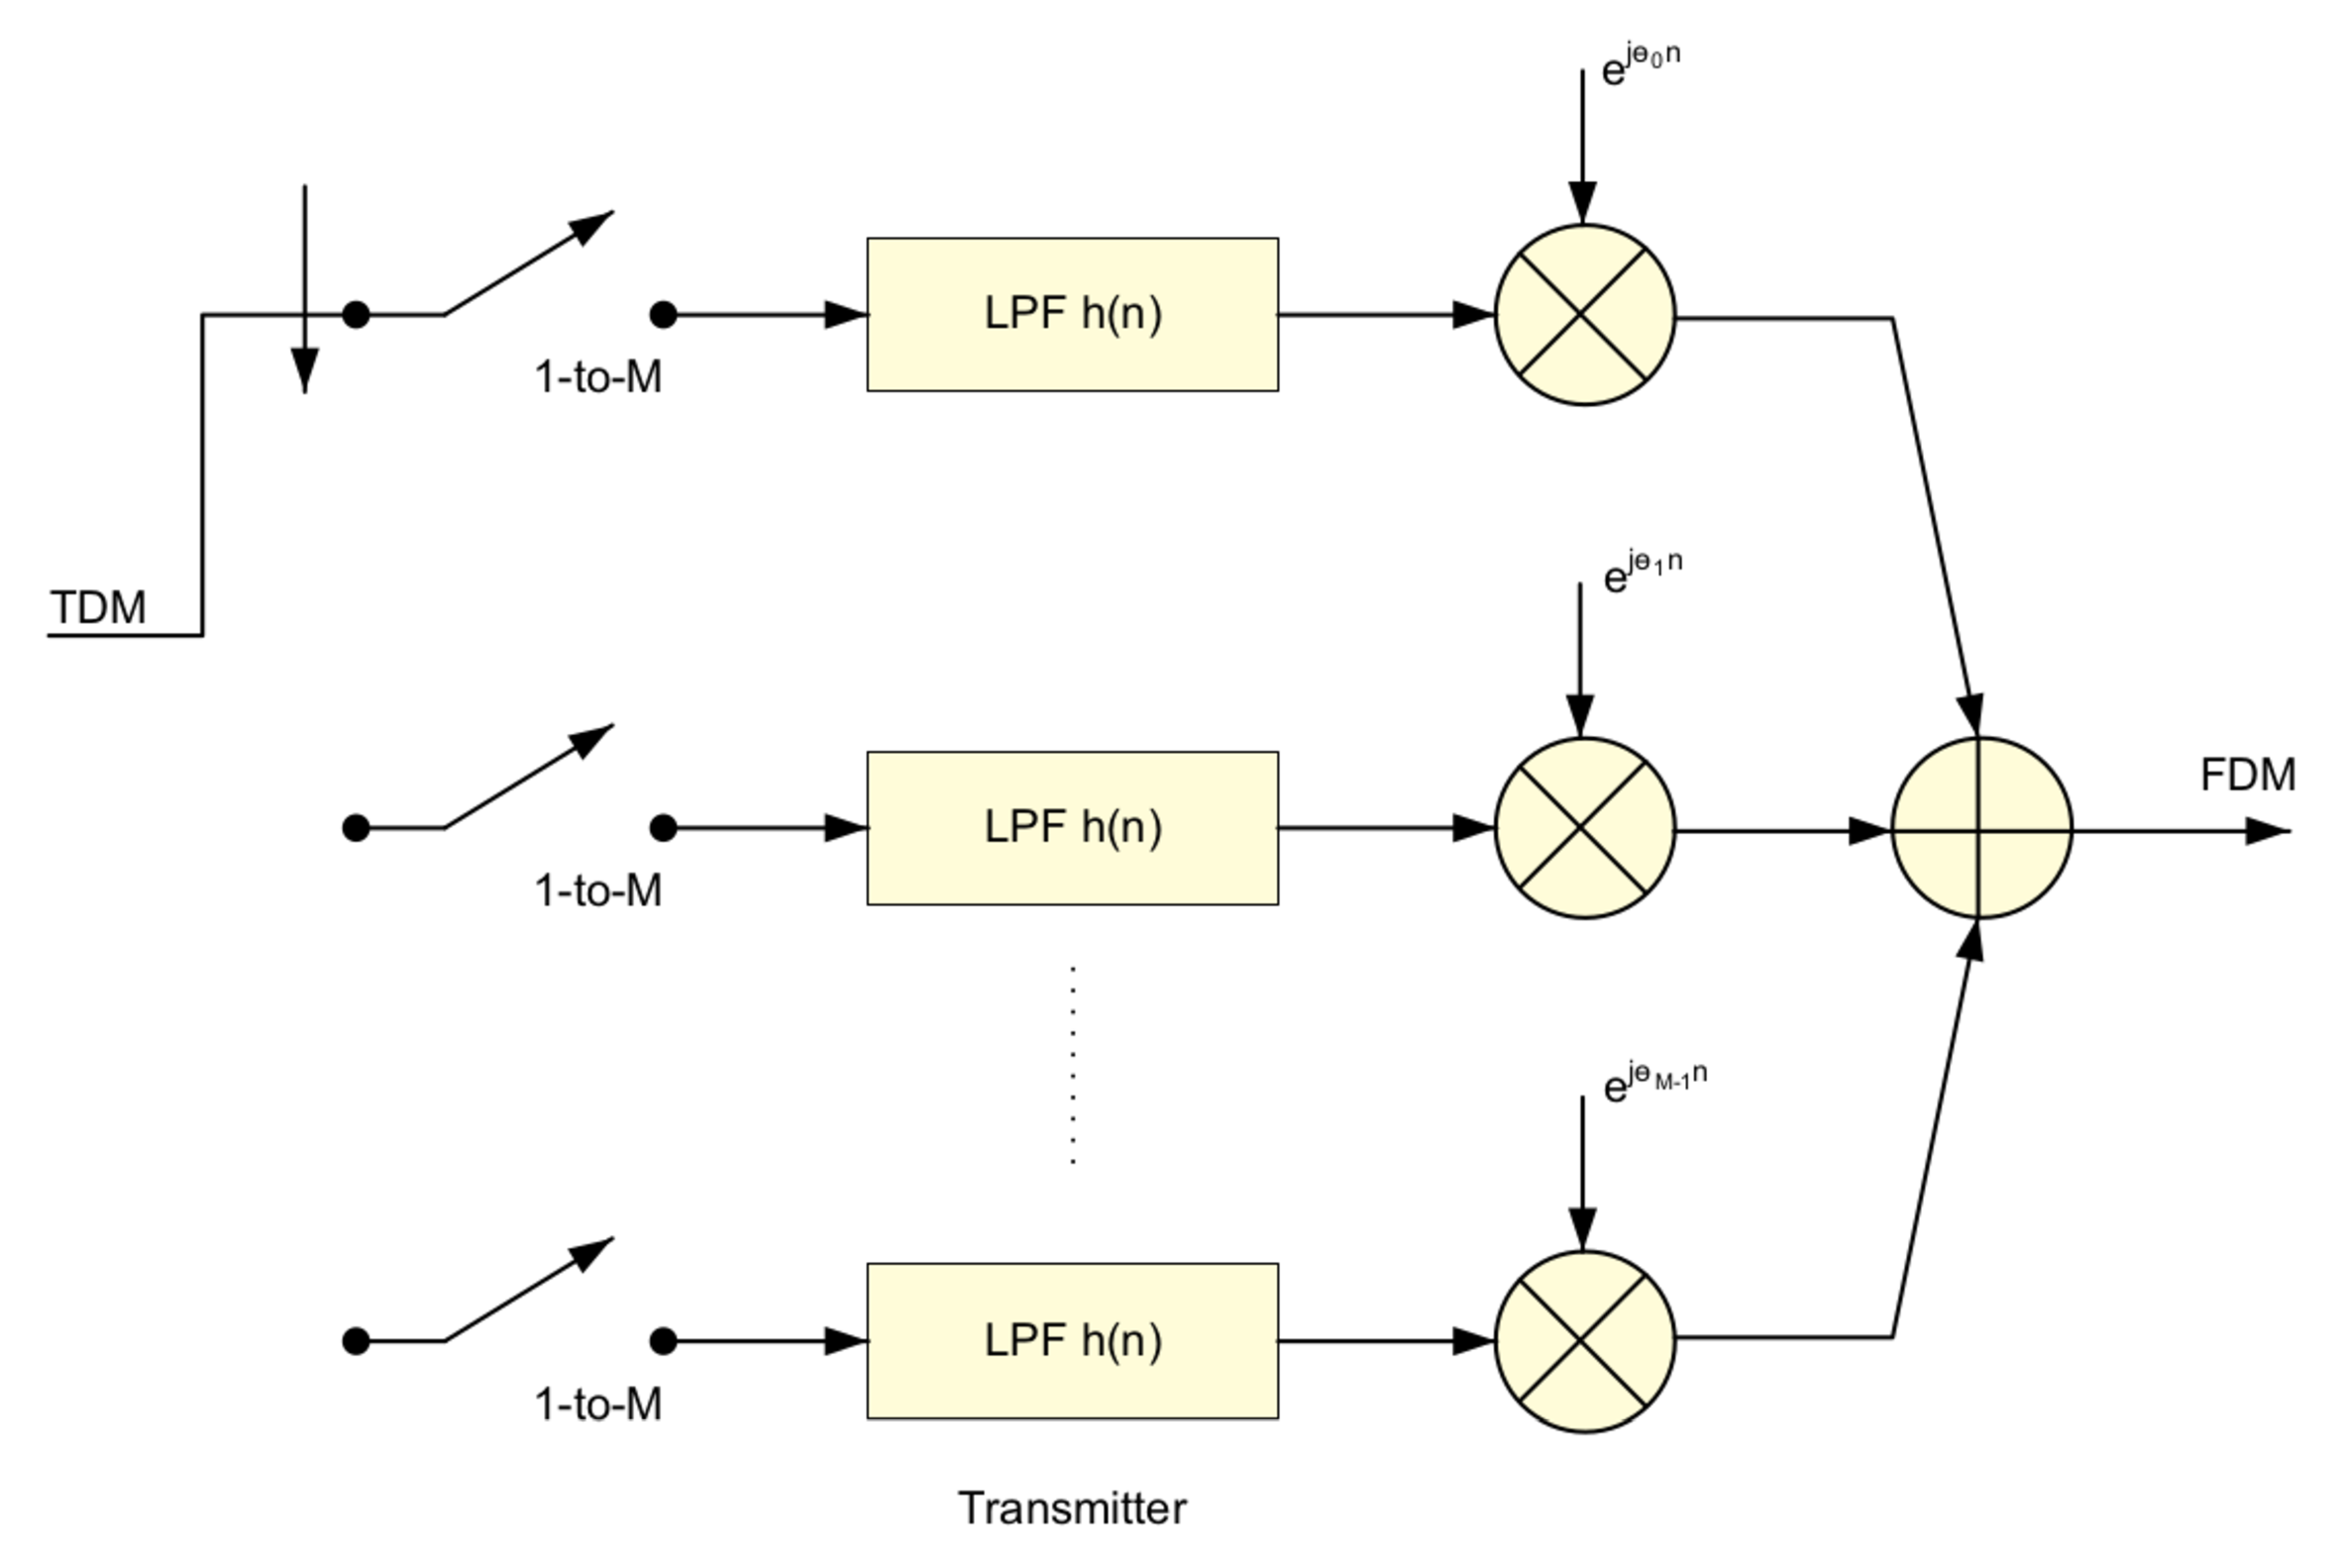
\includegraphics[width=0.8\textwidth]{Tx_channelizer}}
				\end{center}
				%				\end{column}
				%				\begin{column}{0.65\textwidth}
								\begin{center}
												\only<2>{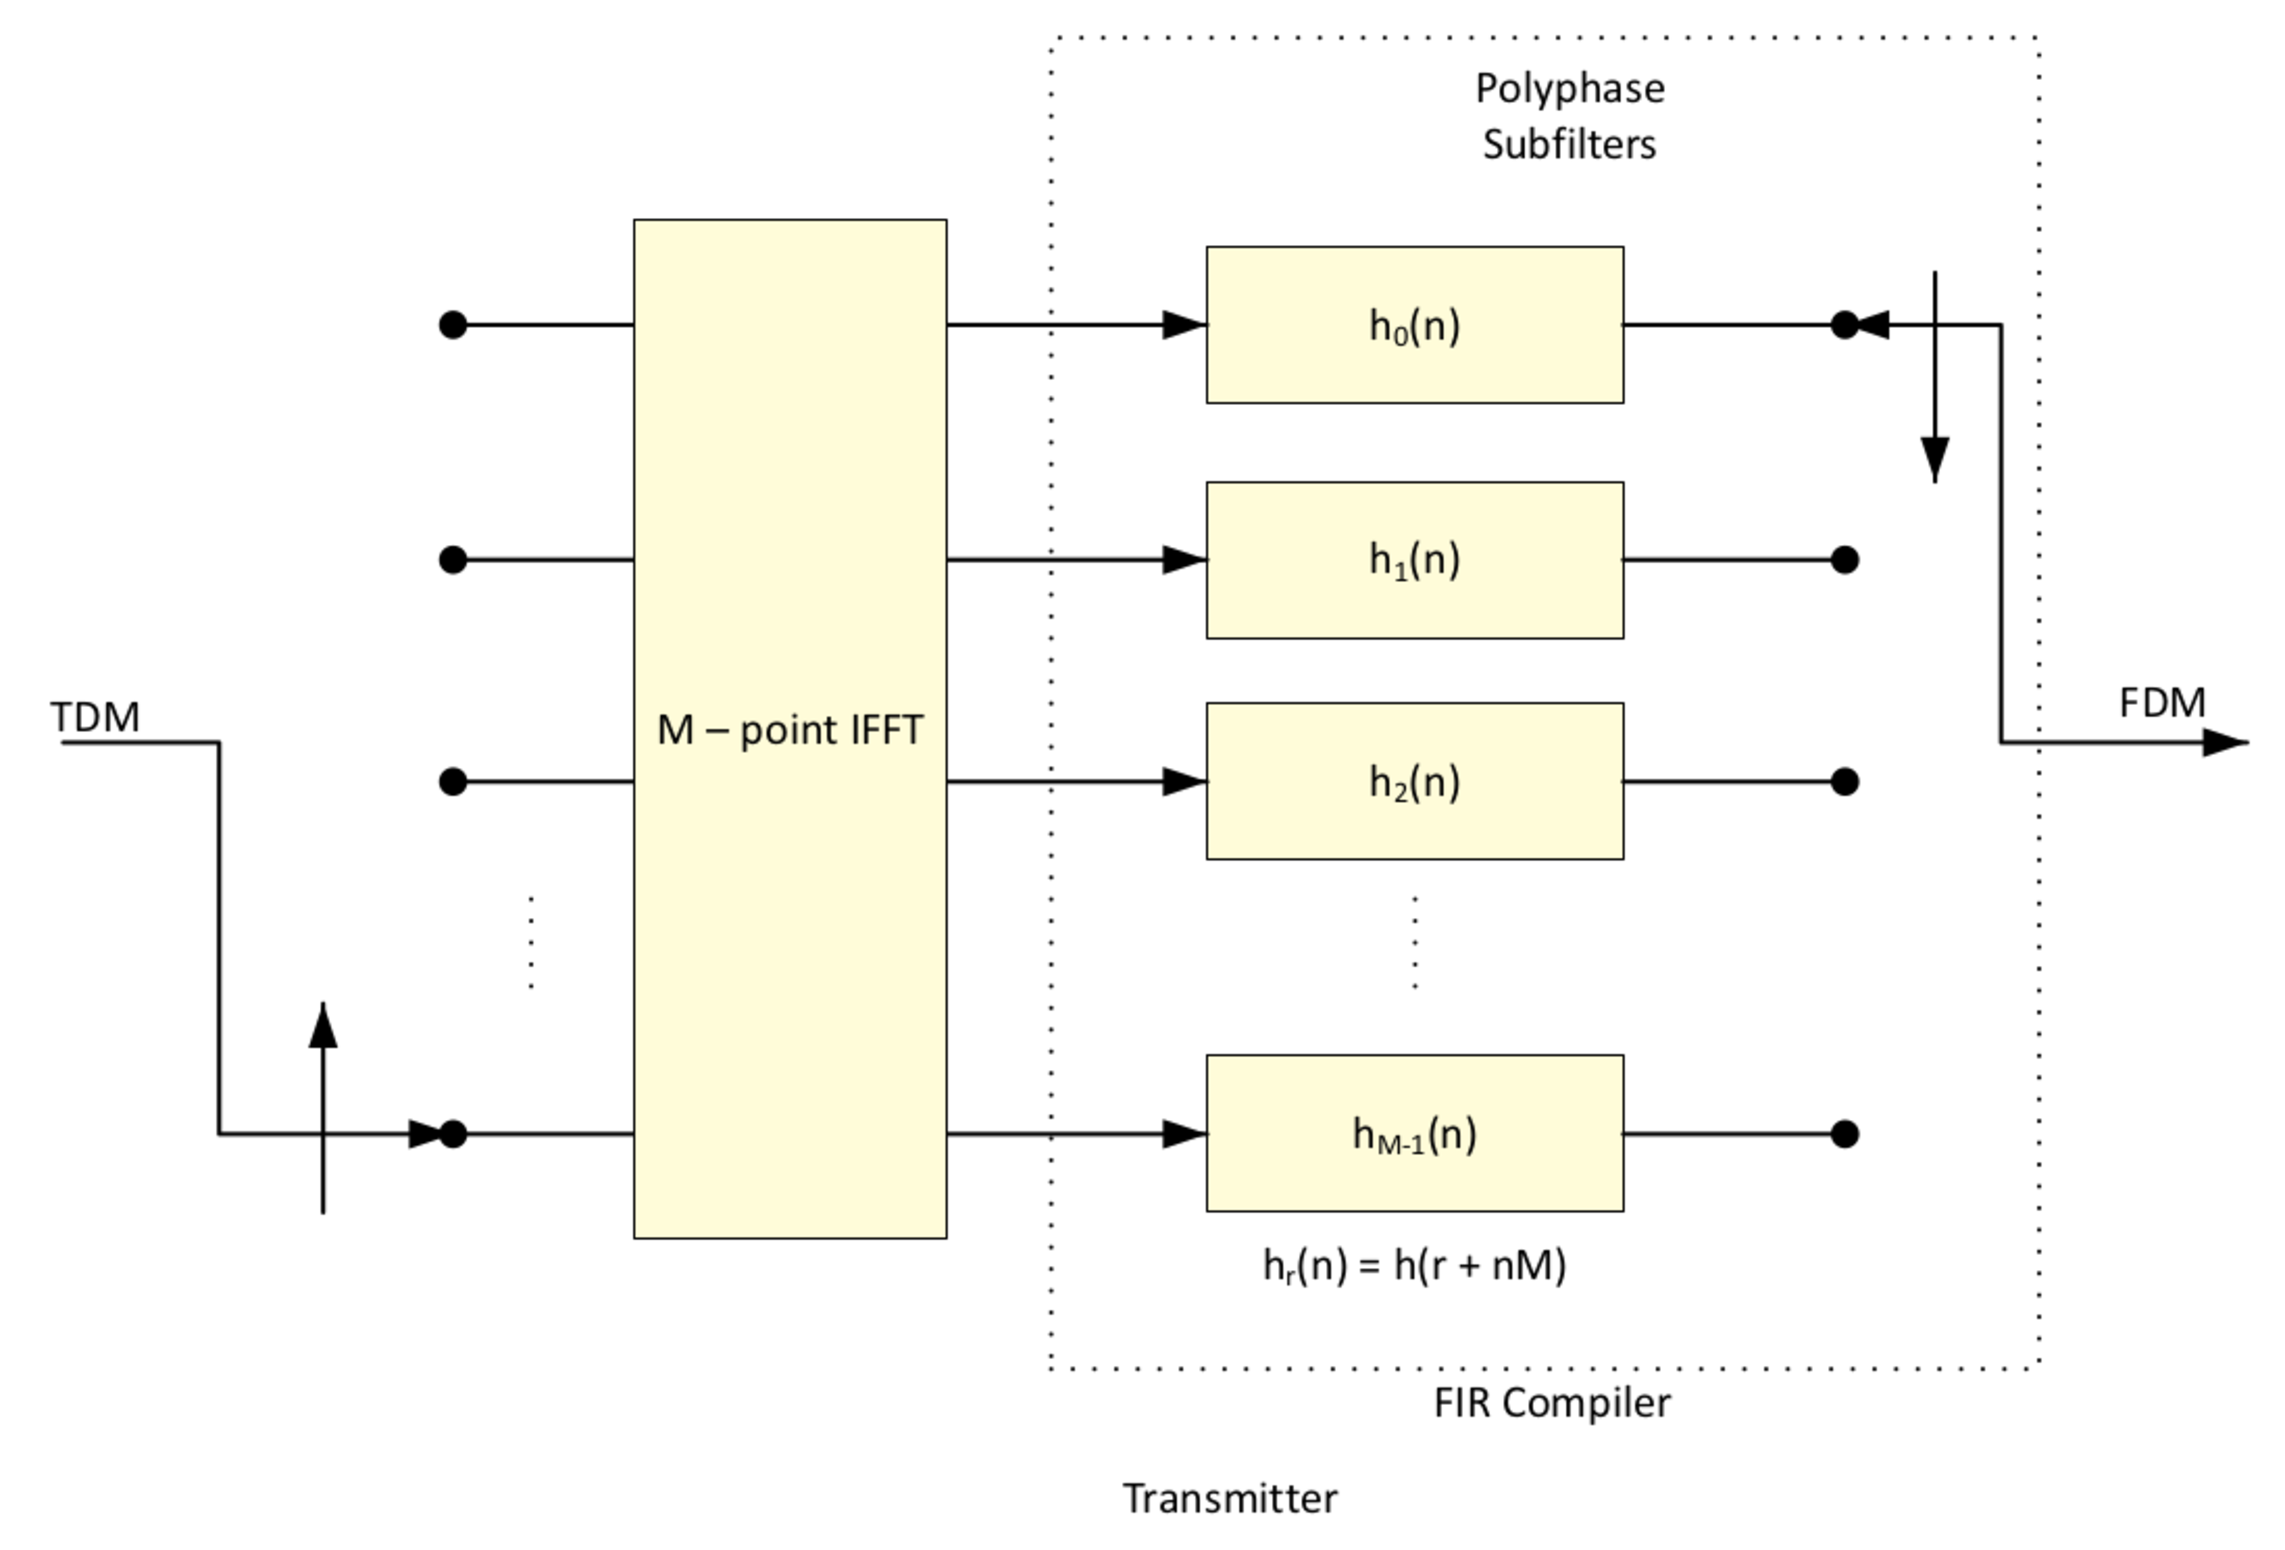
\includegraphics[width=0.8\textwidth]{Tx_channelizer_con_IFFT}}
								\end{center}
								%				\end{column}
								%\end{columns}
\end{frame}
\begin{frame}{Channelizer Rx}
				%\begin{columns}
				%				\begin{column}{0.65\textwidth}
				\begin{center}
								\only<1>{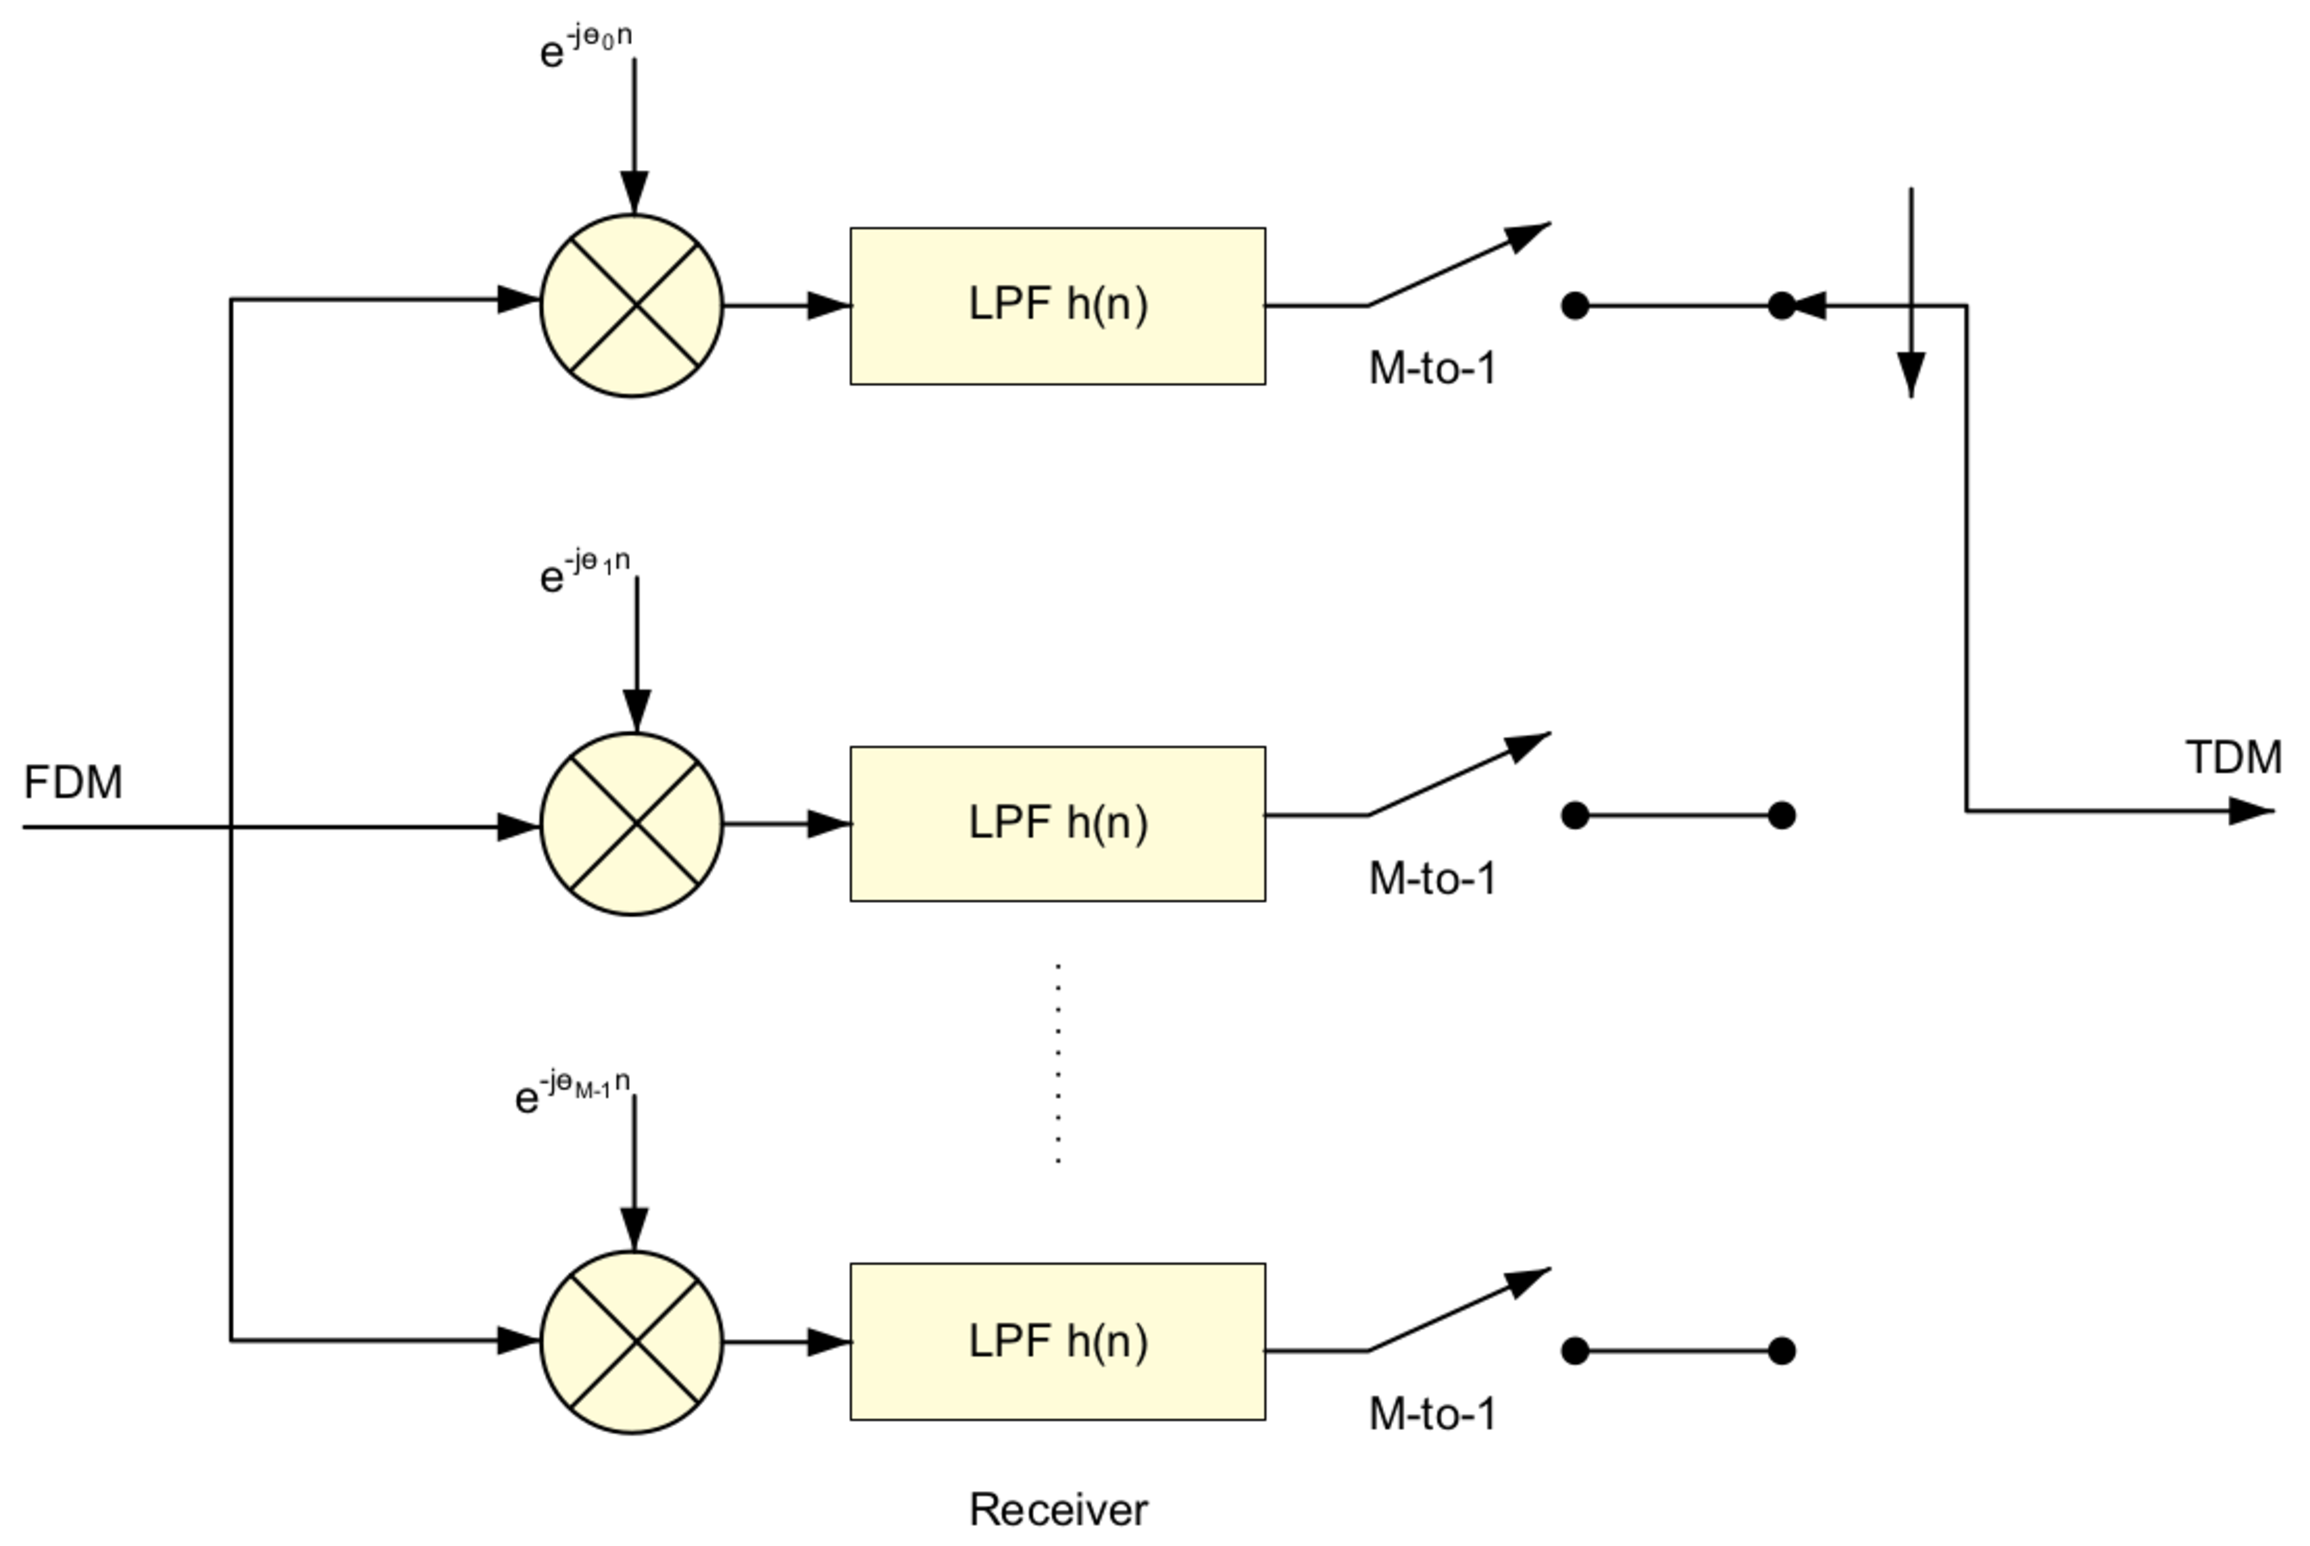
\includegraphics[width=0.8\textwidth]{Rx_channelizer}}
				\end{center}
				%				\end{column}
				%				\begin{column}{0.65\textwidth}
								\begin{center}
												\only<2>{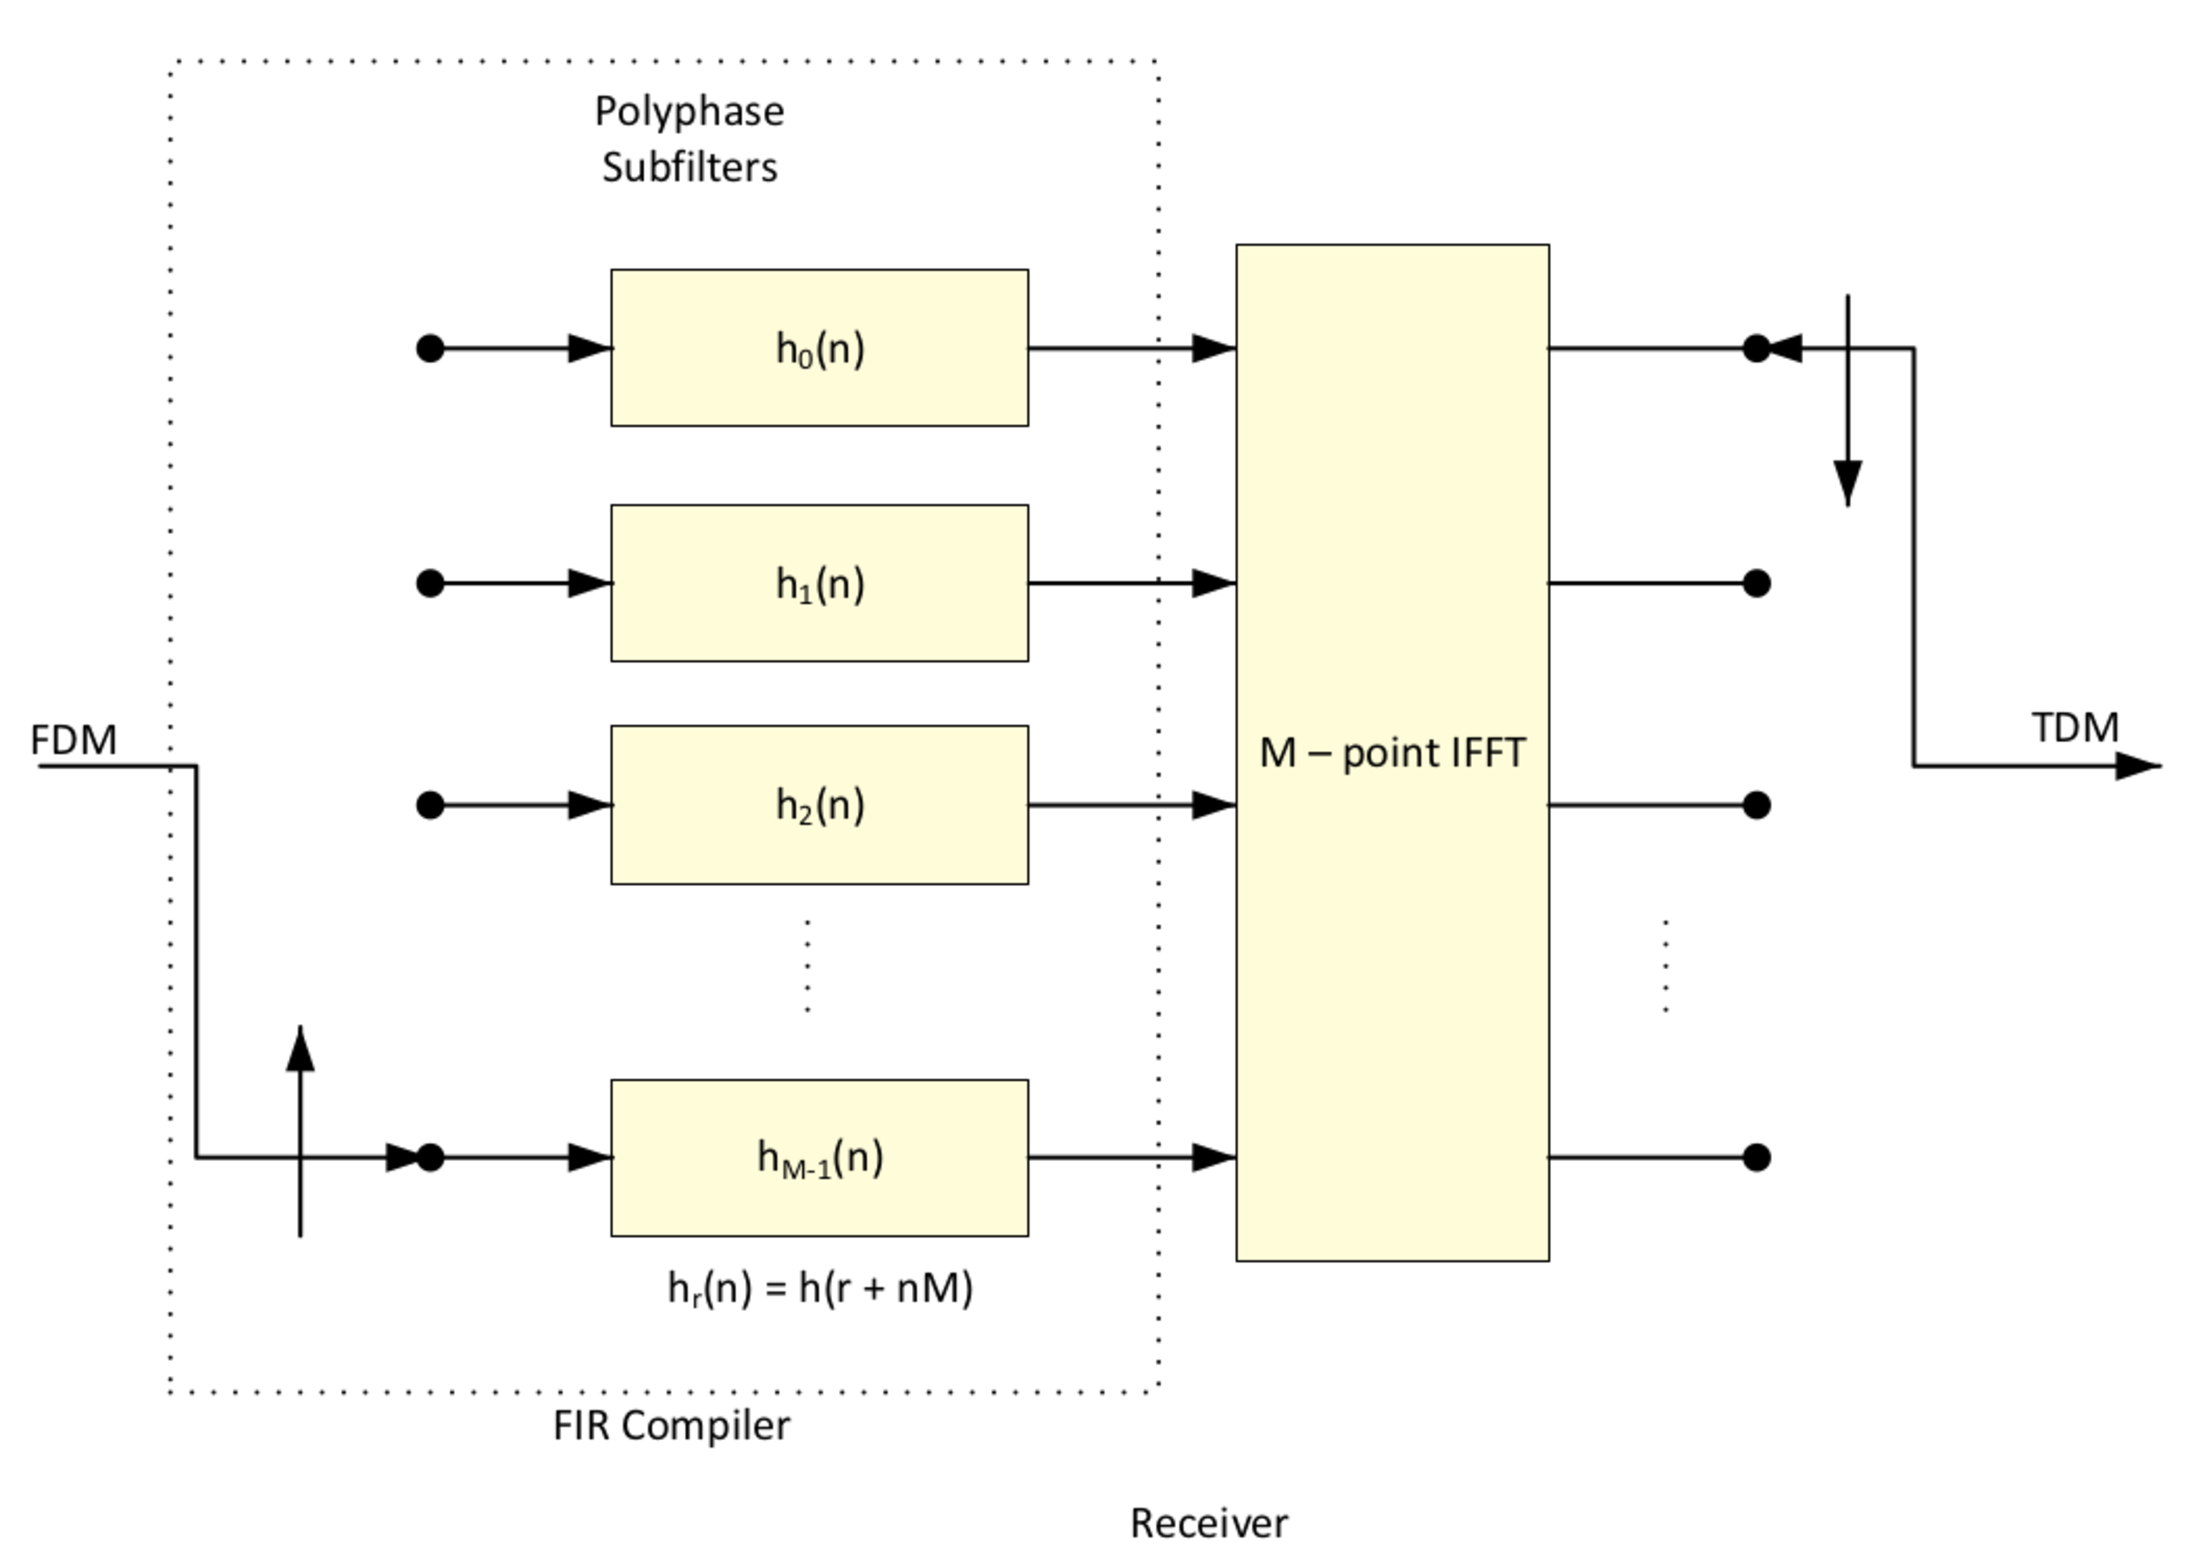
\includegraphics[width=0.8\textwidth]{Rx_channelizer_con_IFFT}}
								\end{center}
								%				\end{column}
								%\end{columns}
\end{frame}
%------------------------------------------------------------------------------
\section{Comparación de arquitecturas de canalización de gran ancho de banda}

\begin{frame}{Digital Down-Converter (DDC)}
				\begin{center}
								\only<1>{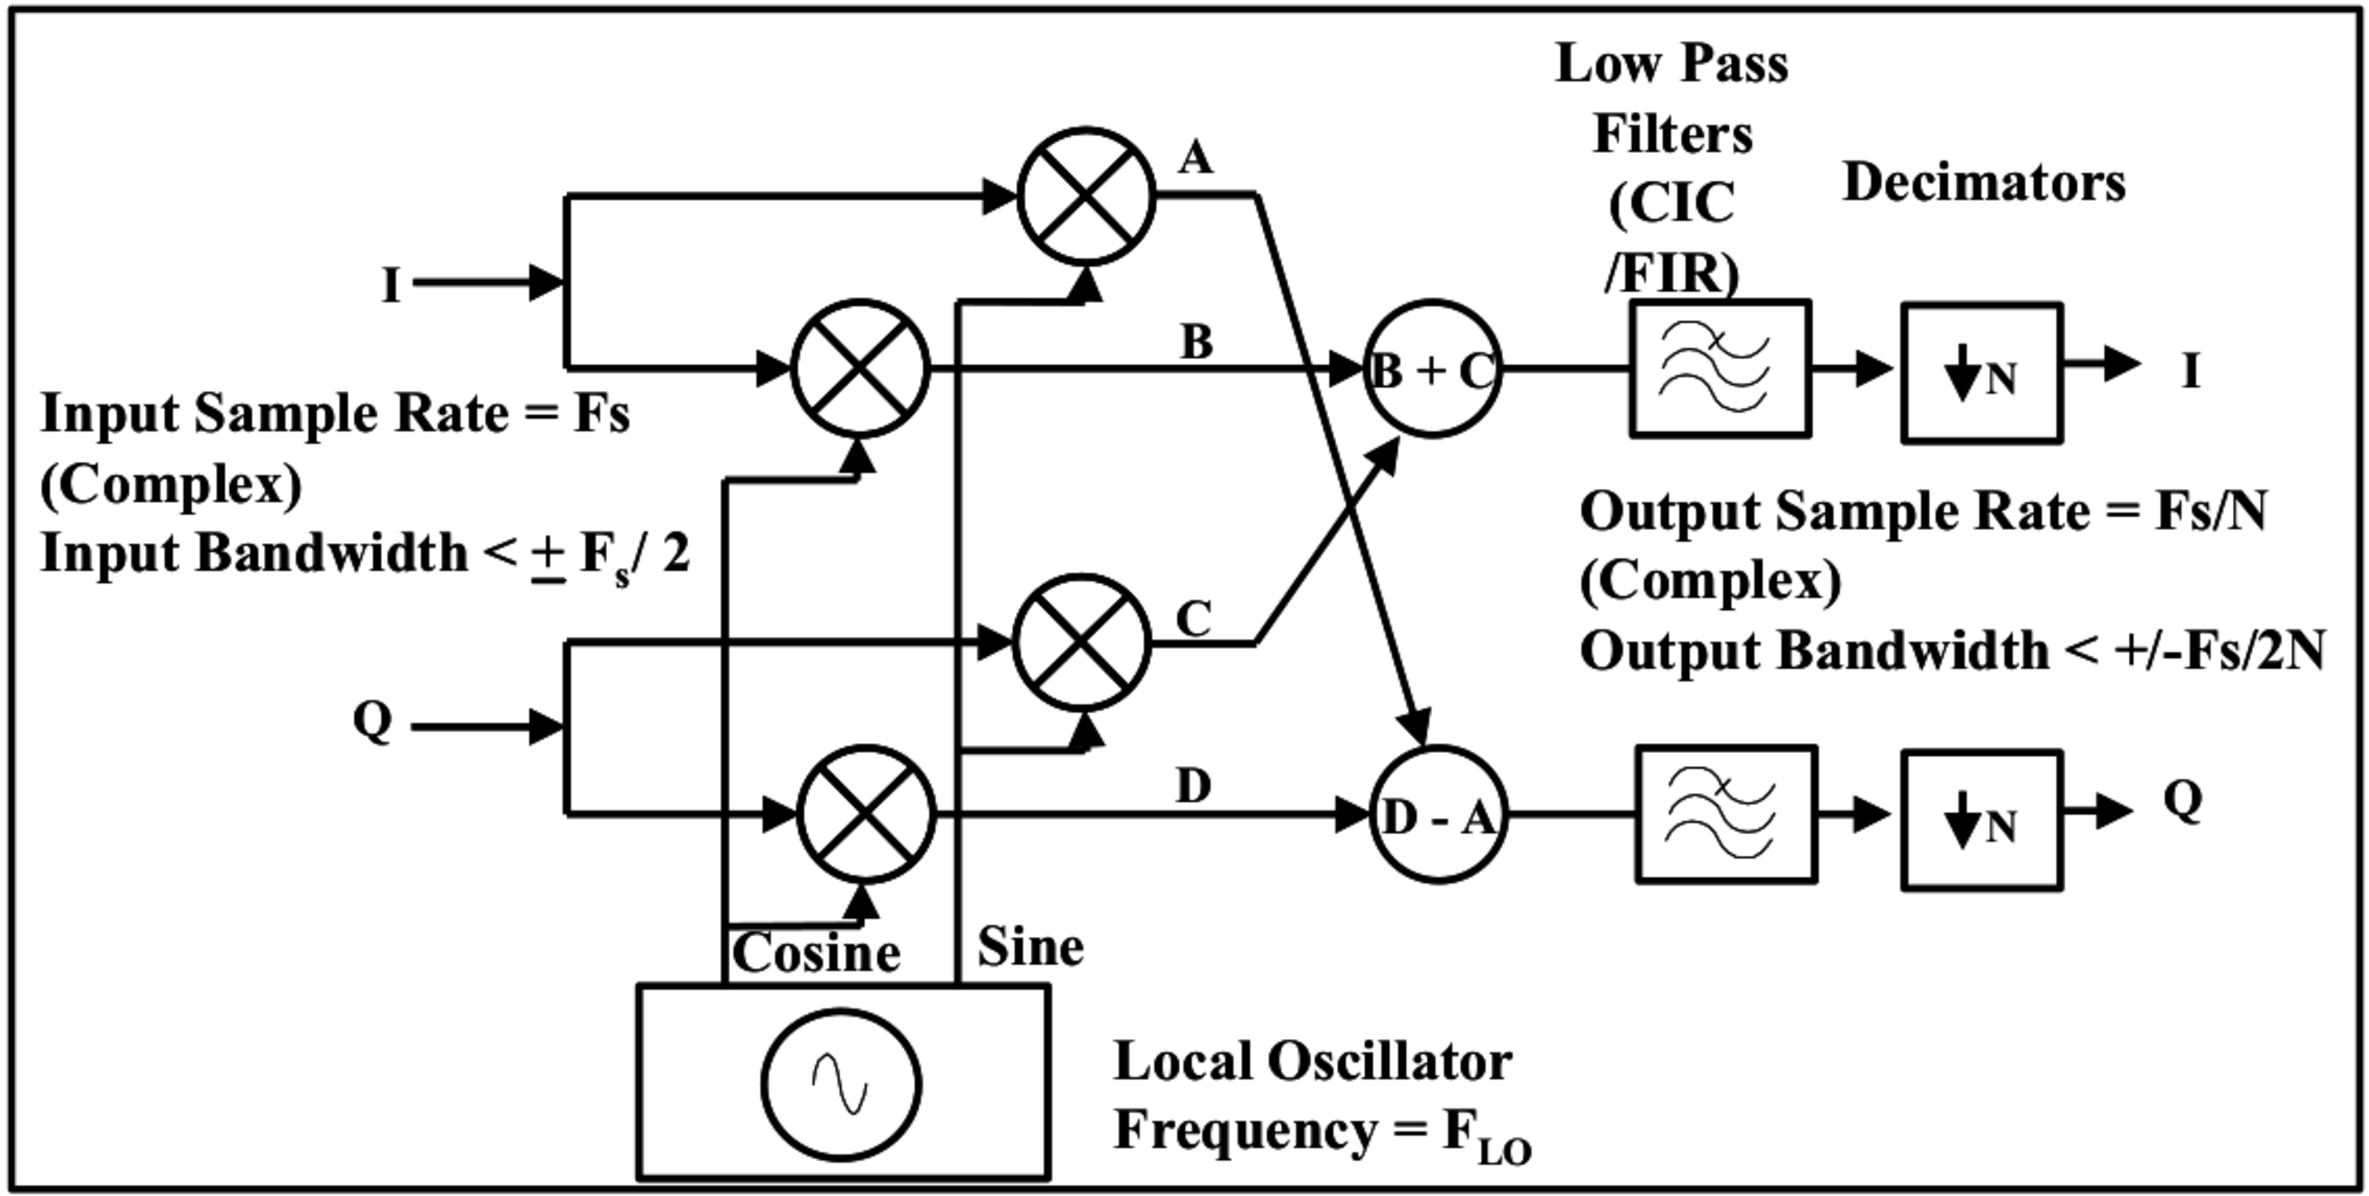
\includegraphics[width=0.9\textwidth]{c1_single_channel_DDC}}
								\only<2>{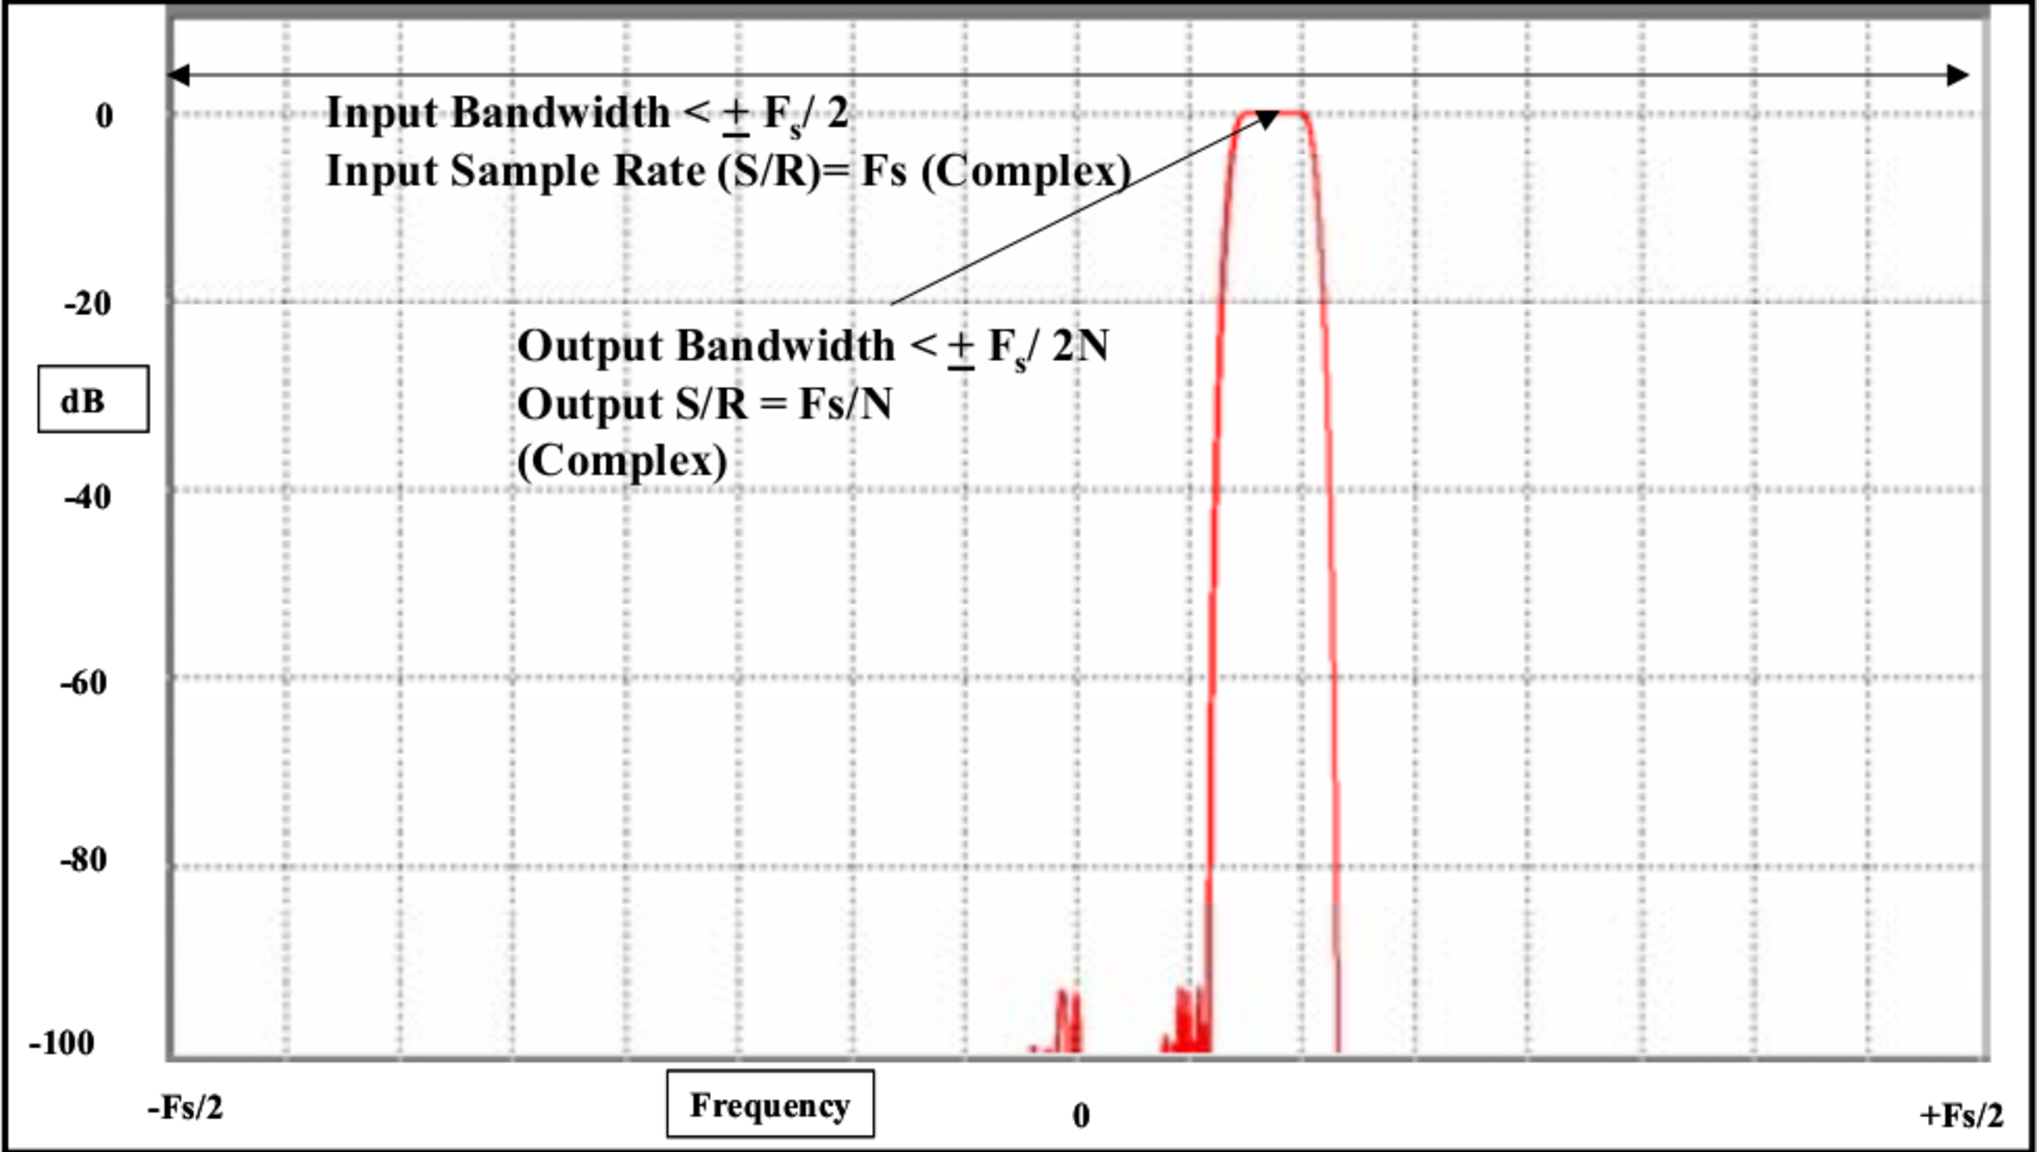
\includegraphics[width=0.9\textwidth]{readout3_compa}}
				\end{center}
								%\begin{center}
								%				\only<2>{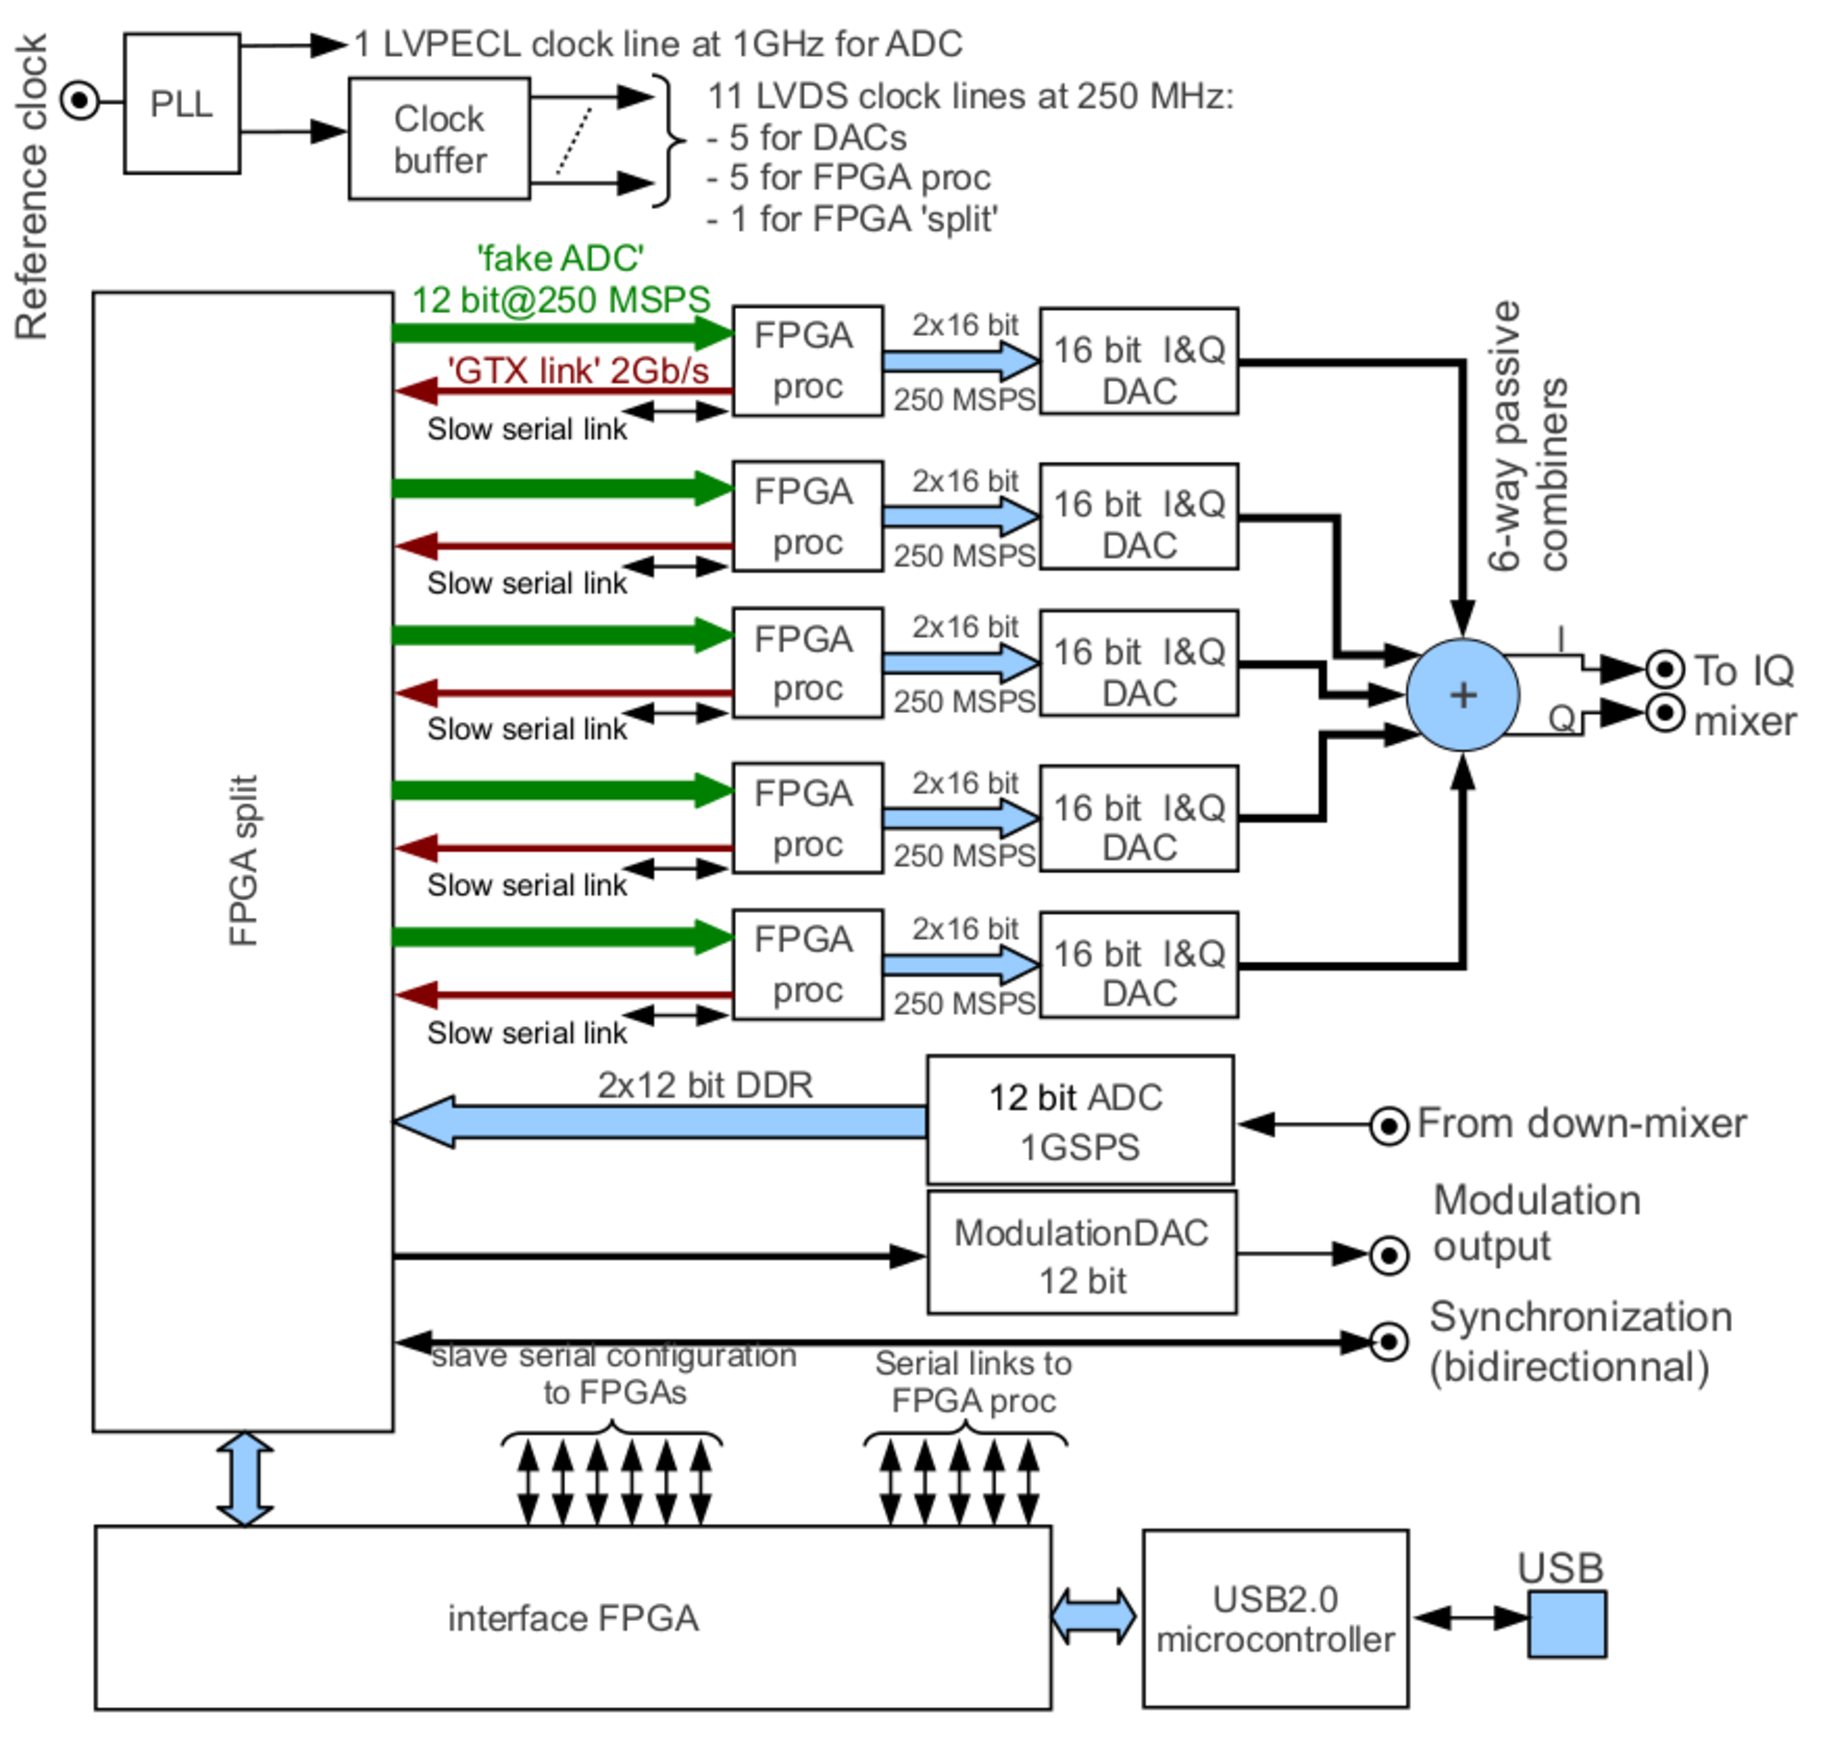
\includegraphics[width=0.5\textwidth]{nikel_readout2}}
								%				\only<2>{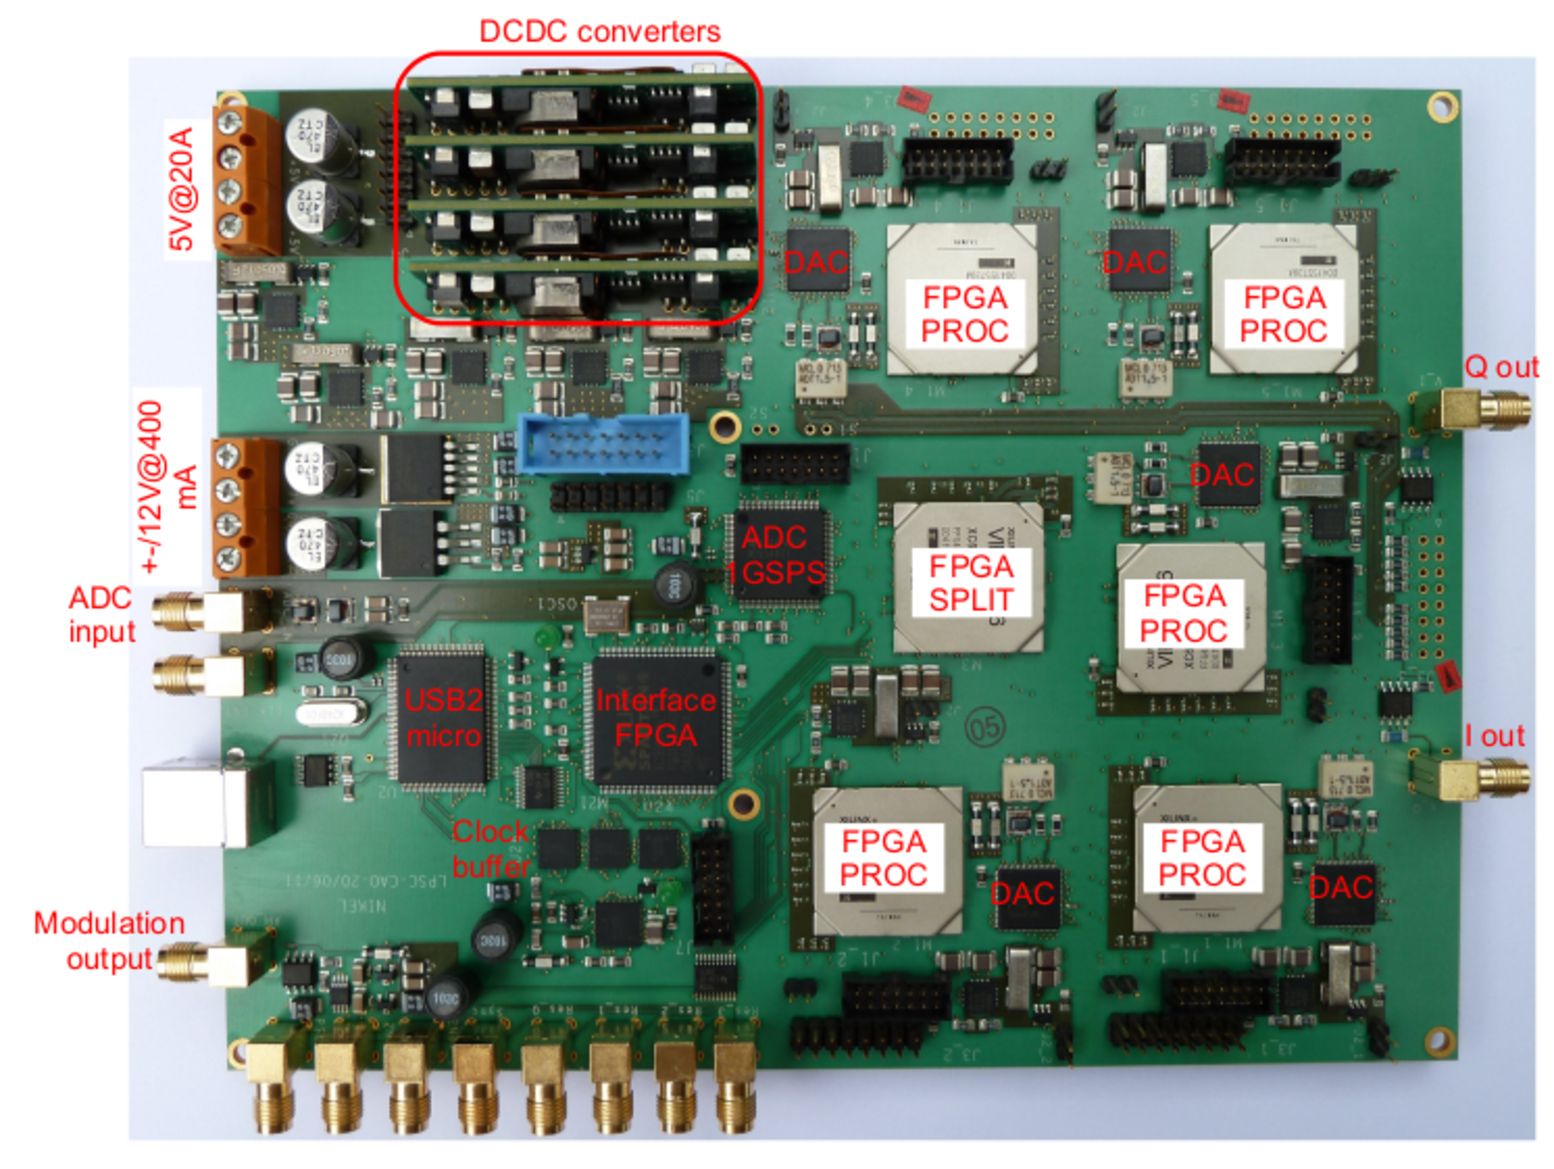
\includegraphics[width=0.5\textwidth]{nikel_readout3}}
								%\end{center}
								Desventaja: los DDC son ``intensivos en silicio'', difícil de
								incluir muchos ($>1000$) canales en FPGA
\end{frame}
\begin{frame}{Arquitectura Pipelined Frequency Transform (PFT)}
				\begin{center}
								\only<1>{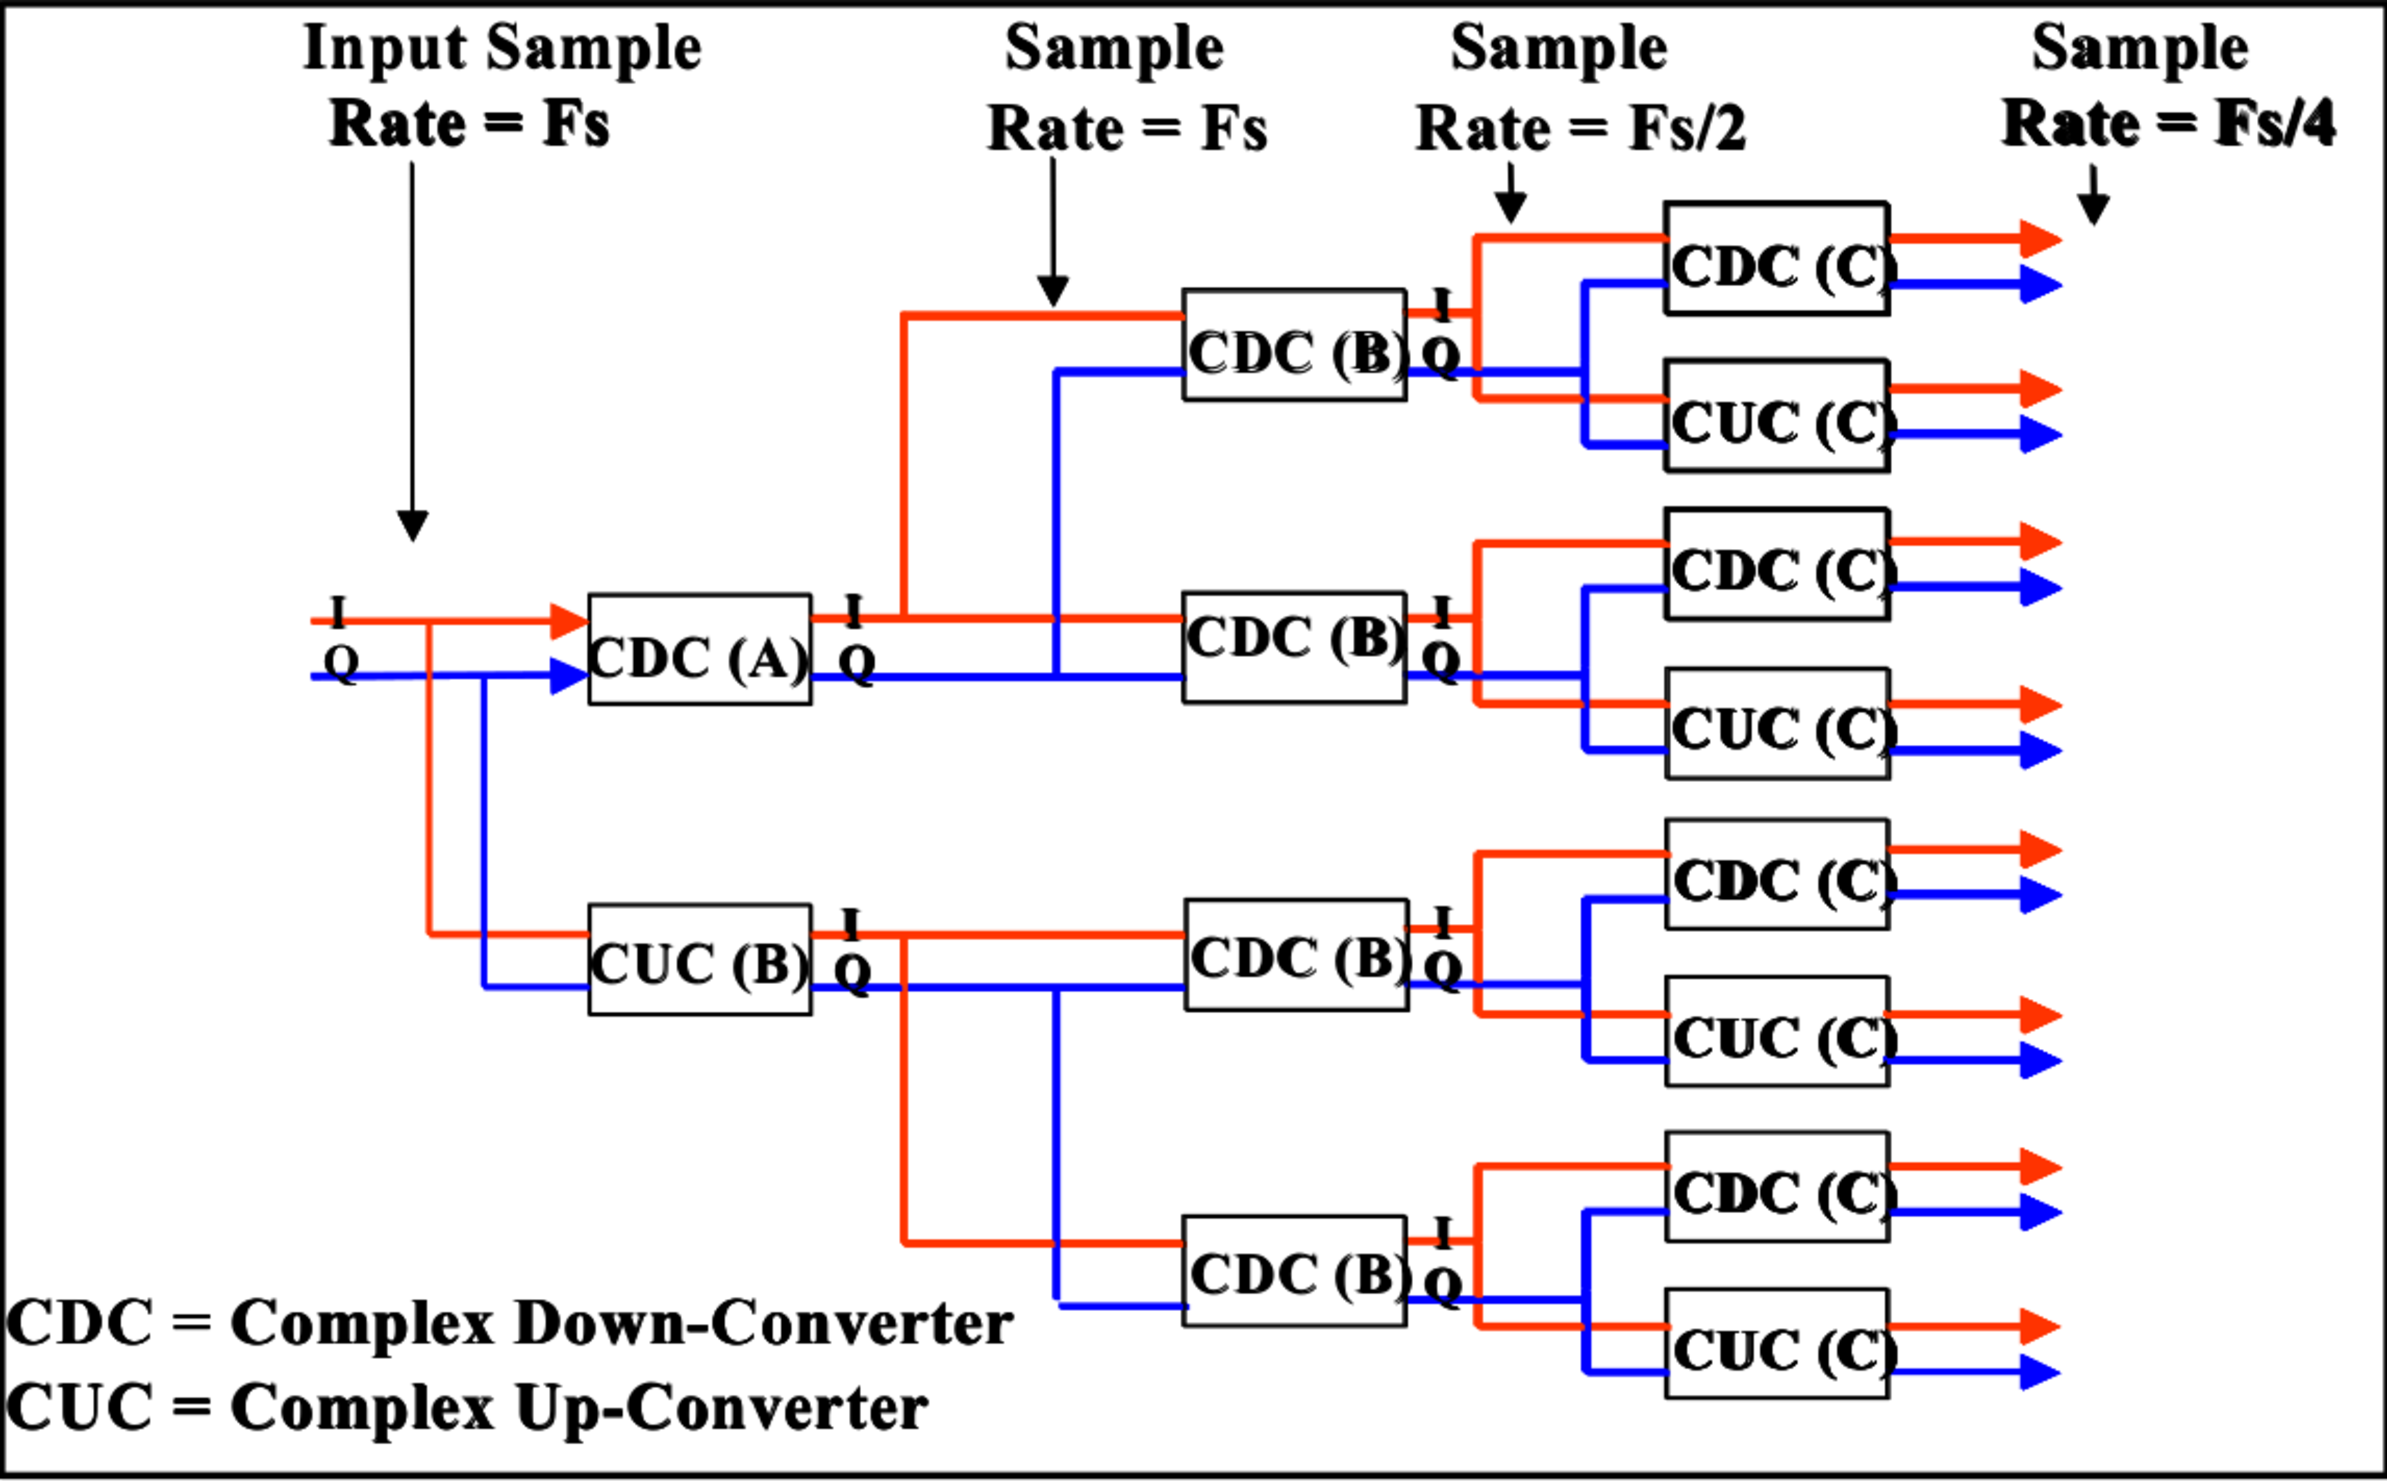
\includegraphics[width=0.45\textwidth]{readout4_compa}}
								\only<1>{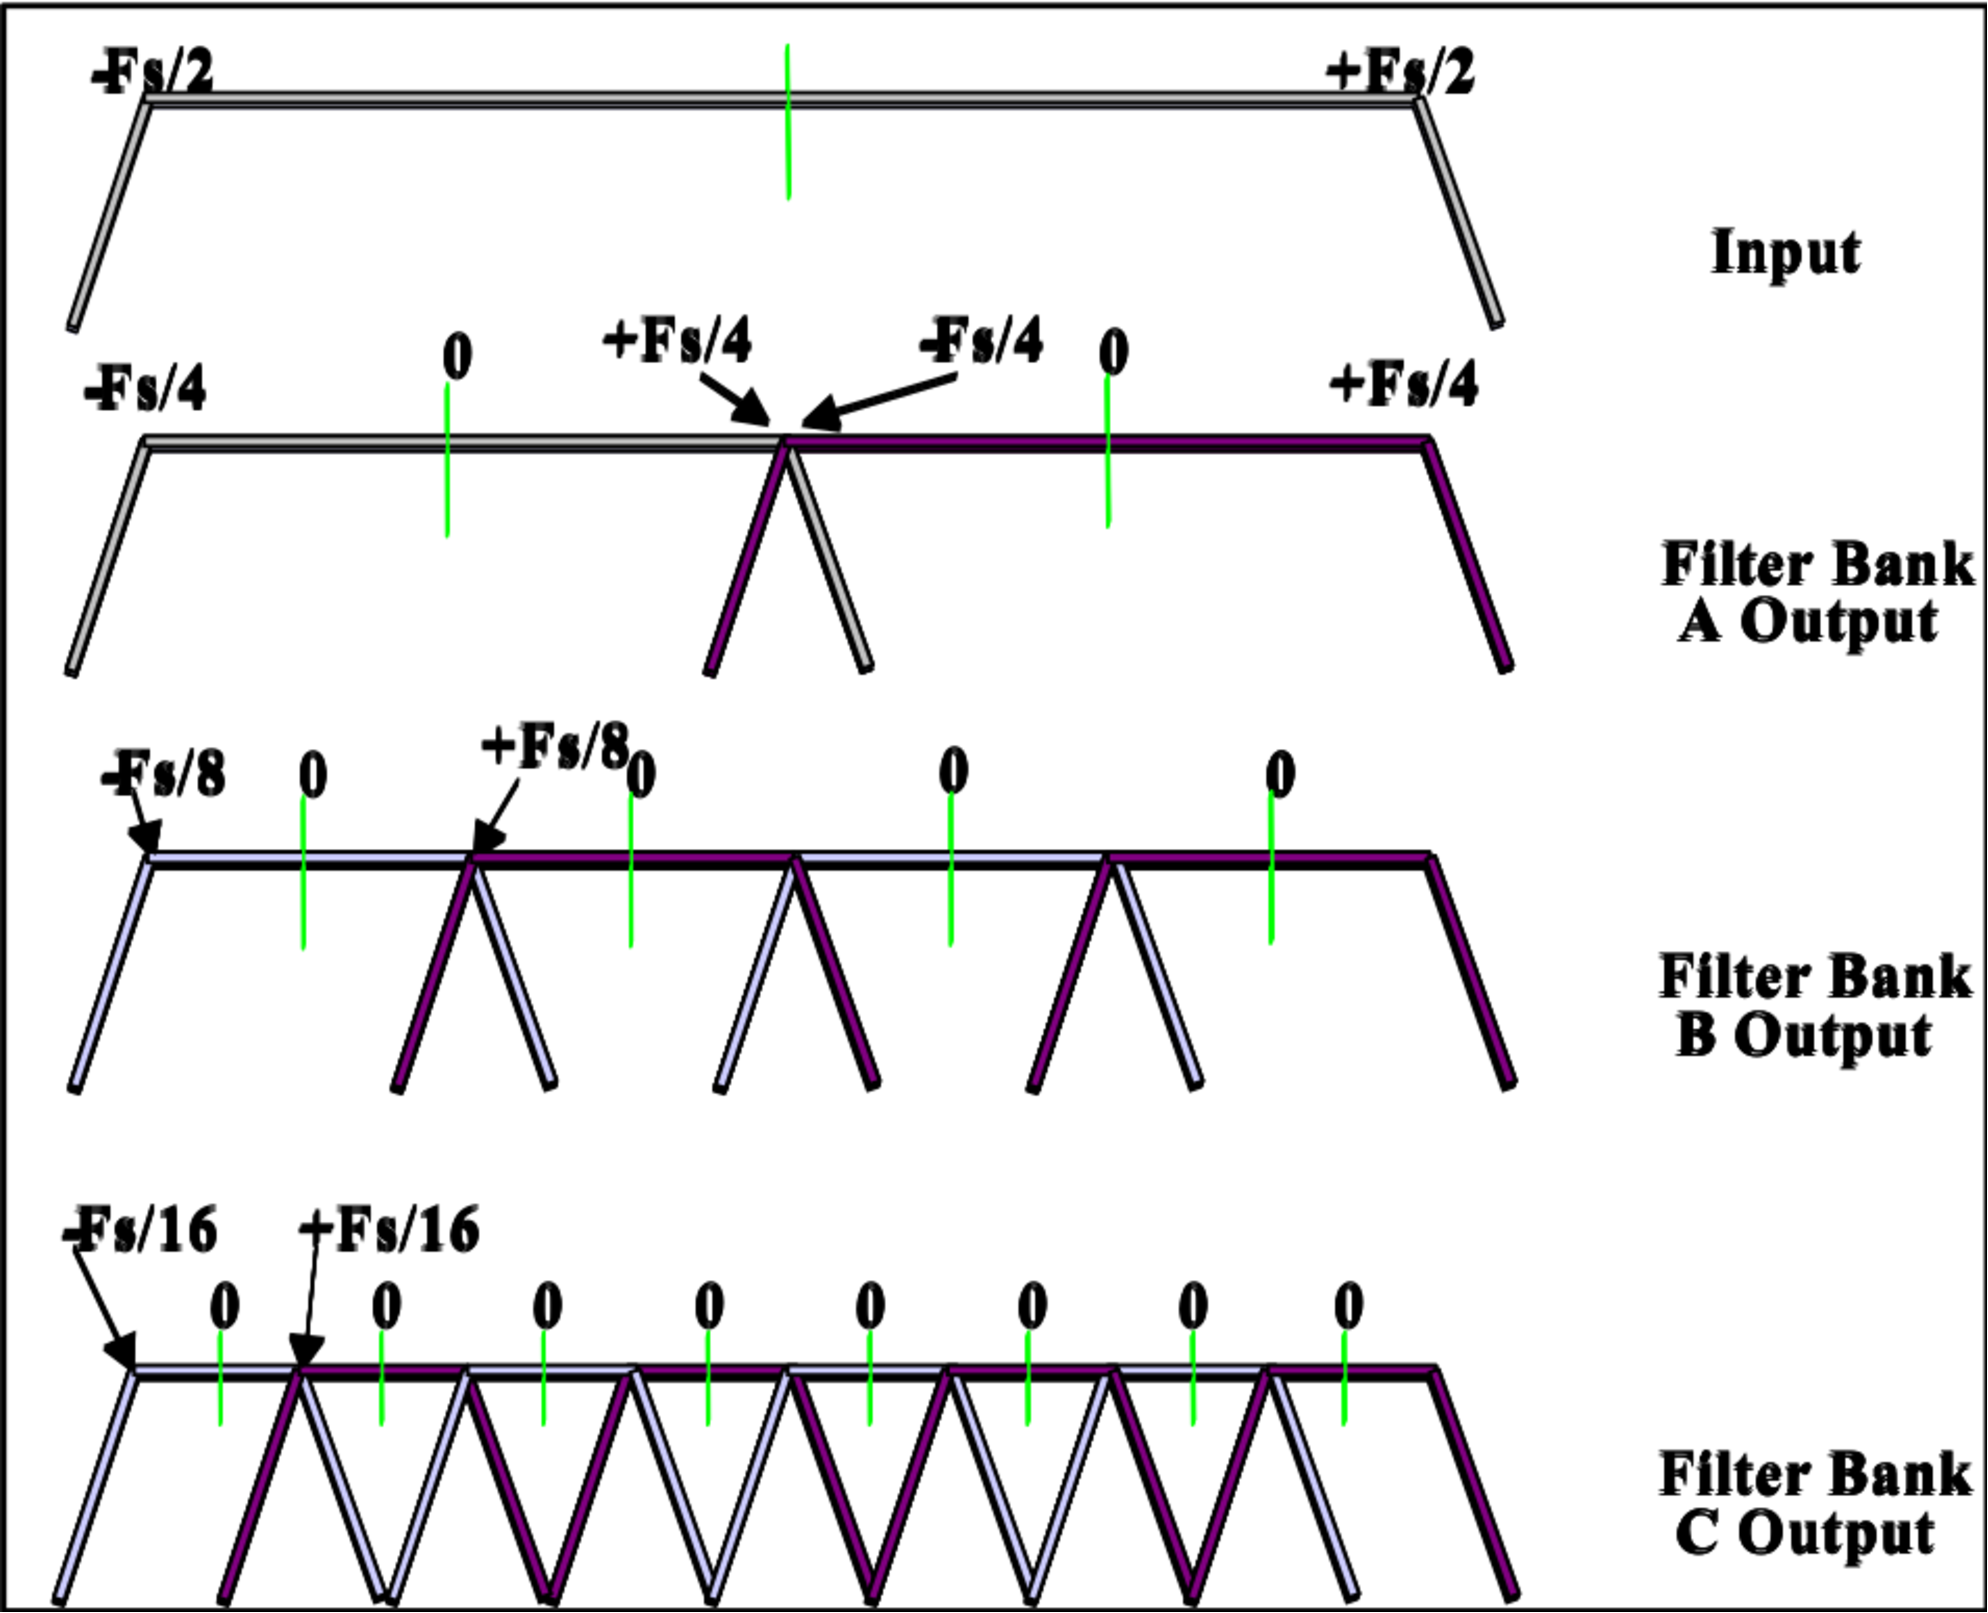
\includegraphics[width=0.35\textwidth]{readout5_compa}}
				\end{center}

				División de bandas de frecuencia $\to$ cada etapa sucesiva de la PFT
				aumenta el número de bandas en un factor de dos

				Desventaja: para un gran número de canales ($>1000$), el árbol se vuelve
				muy grande. Por ejemplo, 1024 canales requerirían 2046 módulos (CDC o
				CUC) complejos
\end{frame}

\begin{frame}{Arquitectura DFT Polifase}
				\begin{center}
								\only<1>{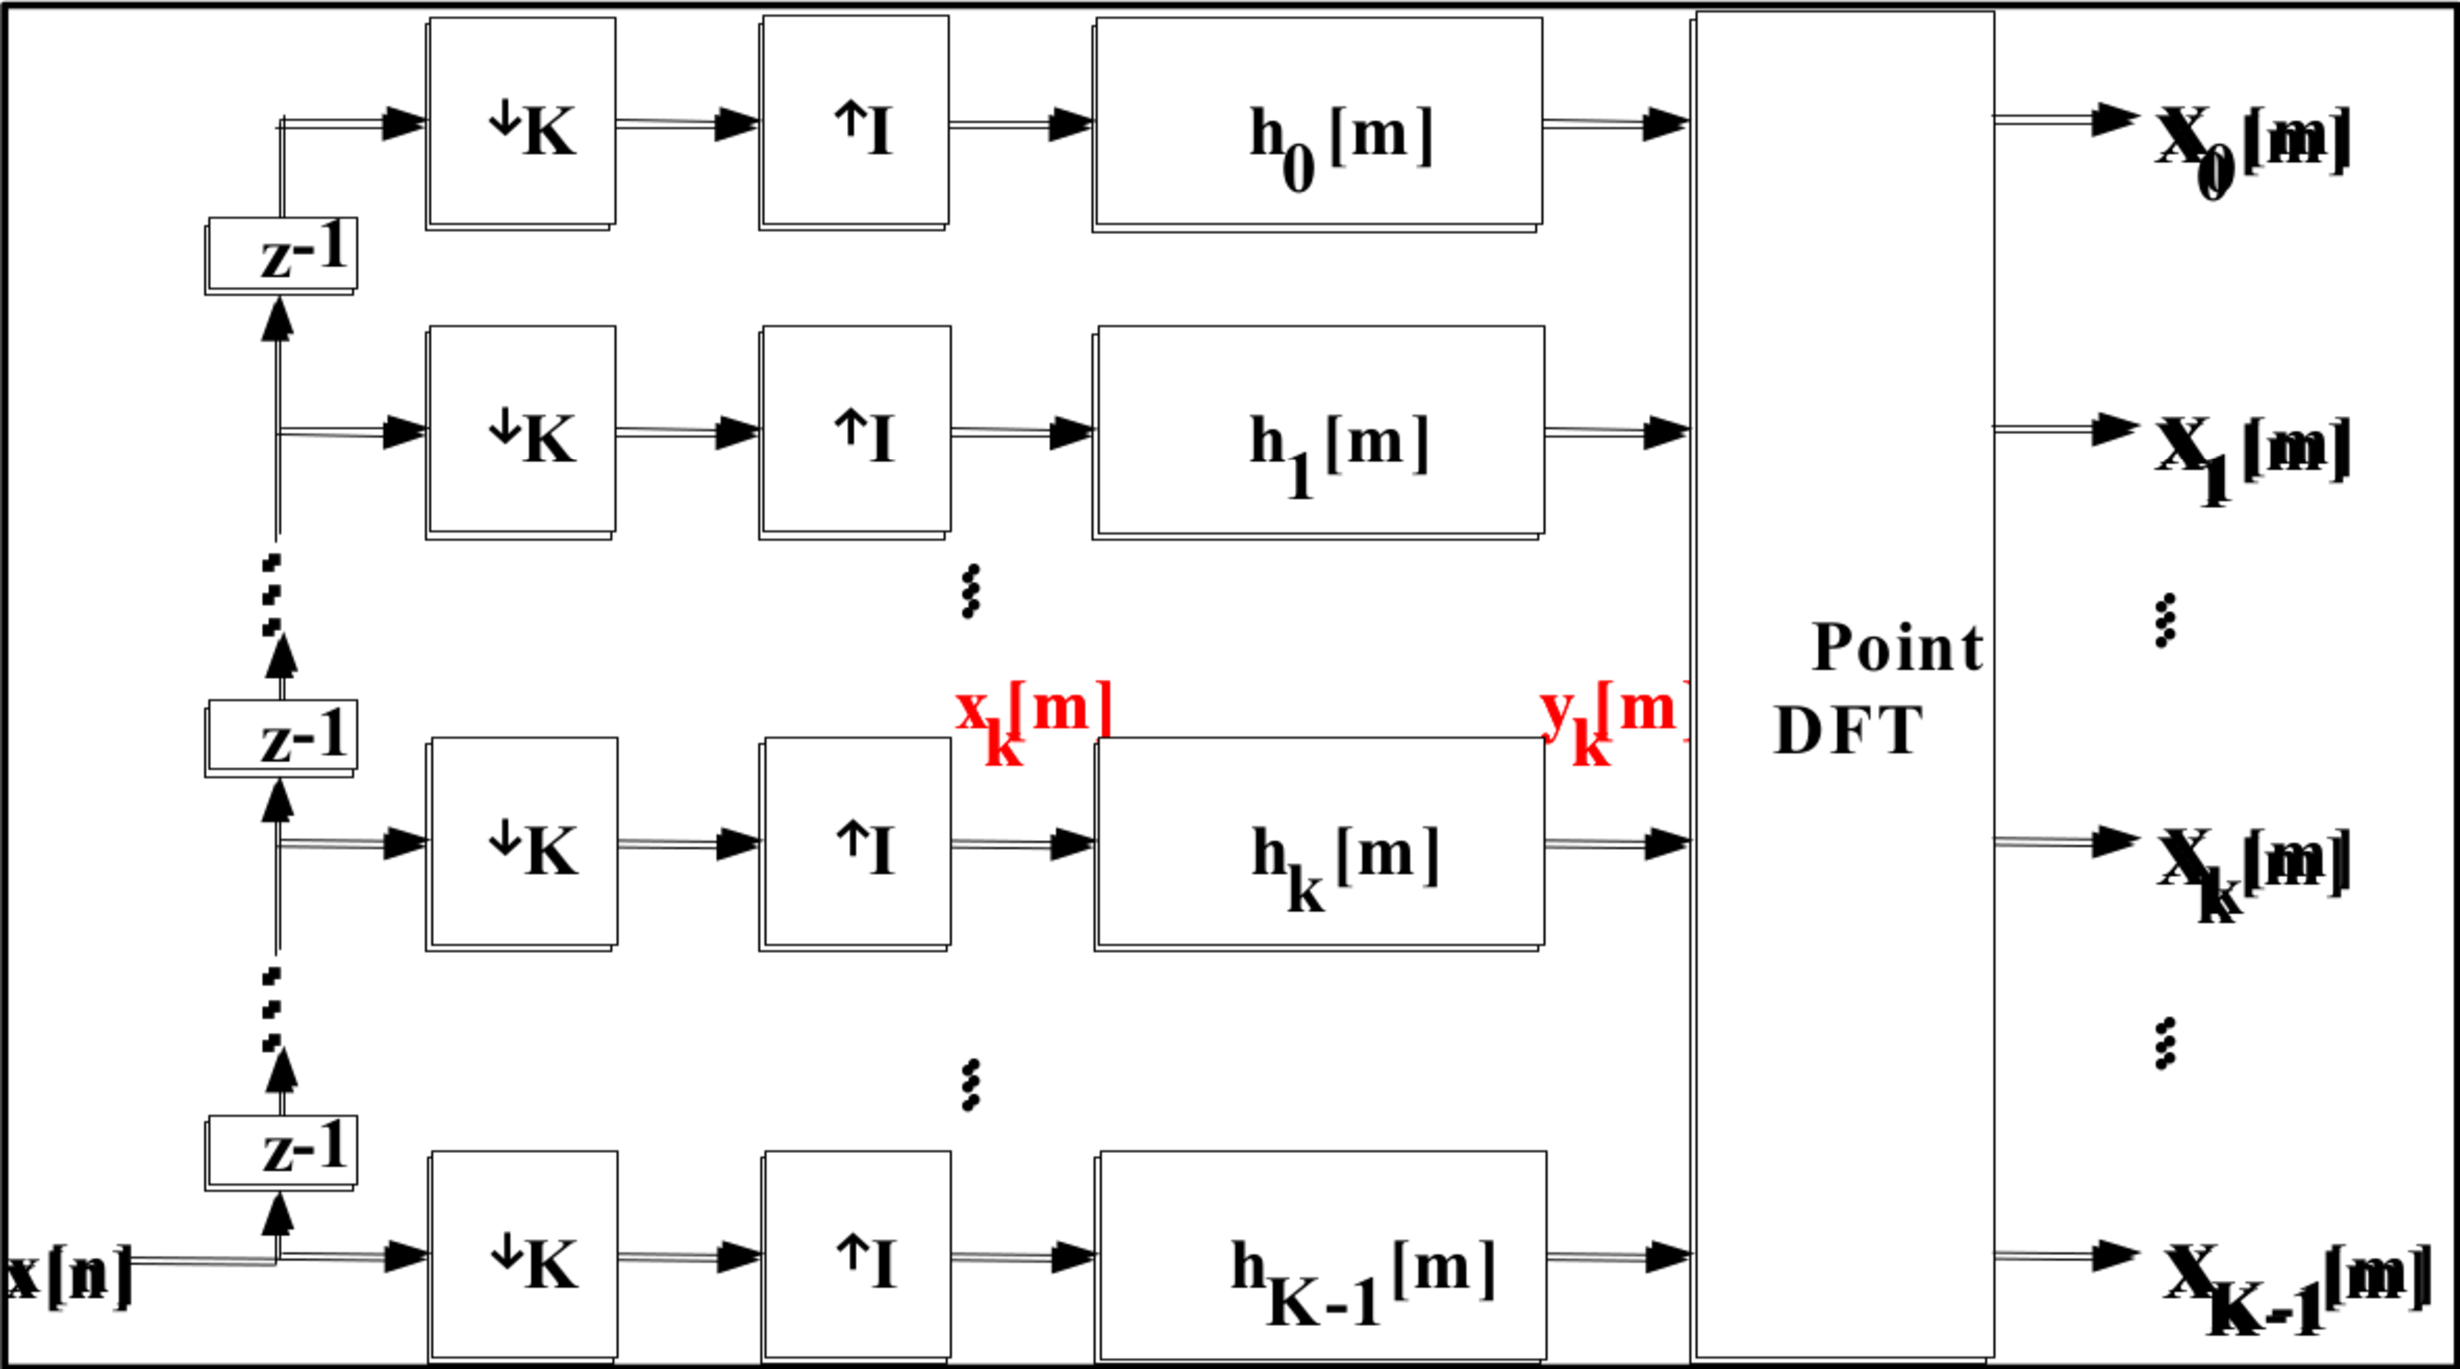
\includegraphics[width=0.47\textwidth]{readout6_compa}}
								\only<1>{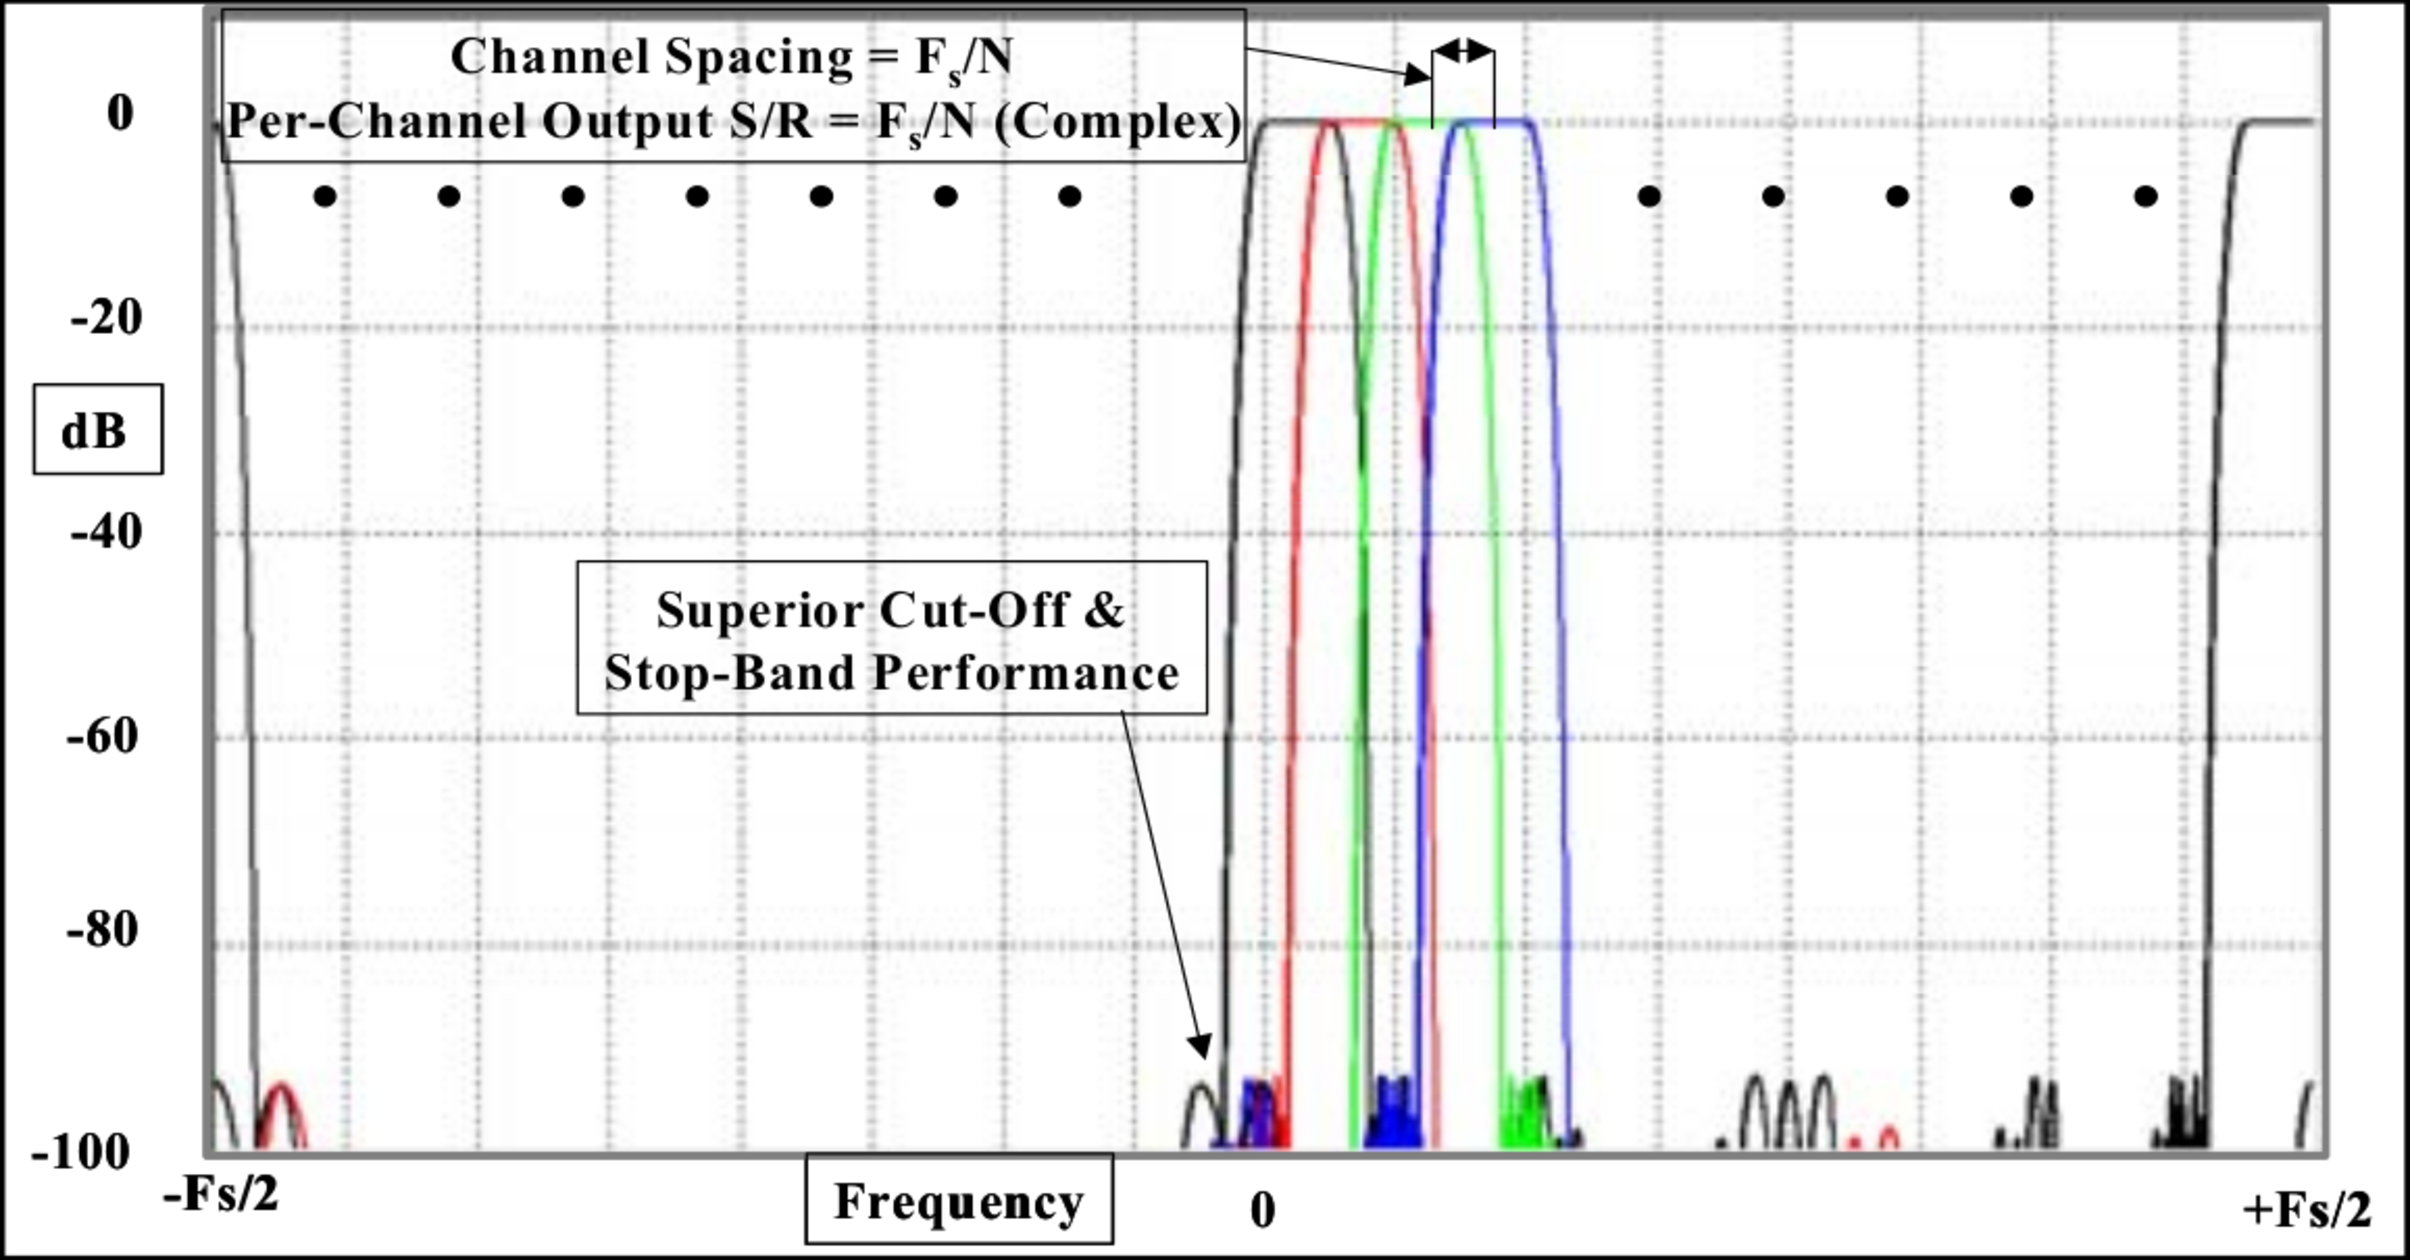
\includegraphics[width=0.50\textwidth]{readout7_compa}}
				\end{center}

				$M = K \to$ críticamente muestreado

				$M < K (I = K/M) \to$ caso sobre-muestreado (oversampled)

				Para nuestra aplicación $I=2$ es una elección \alert{adecuada y
				suficiente}

				Arquitectura conveniente para cuando el número de canales es grande

\end{frame}

\begin{frame}{Canalizador FFT}
				\centering
								\only<1>{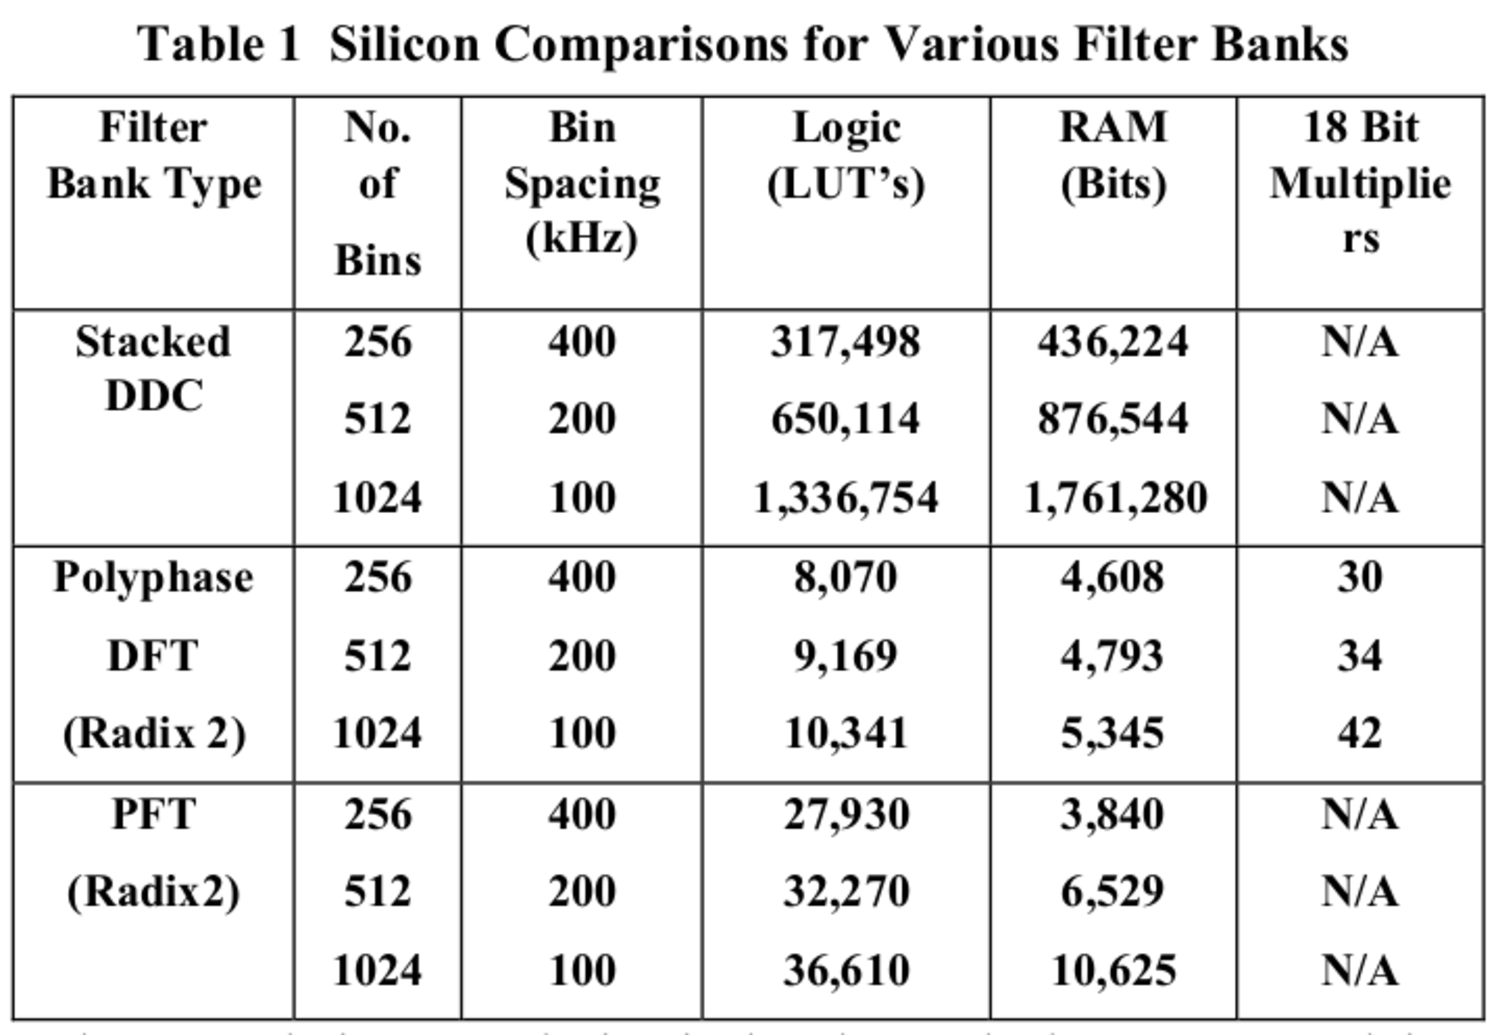
\includegraphics[width=0.5\textwidth]{readout2_tabla_compa}}
				\only<2>{\begin{overpic}[width=0.5\textwidth]{readout2_tabla_compa}
								\put(0,16){\color{red}\rule{180pt}{1pt}}
								\put(0,32){\color{red}\rule{180pt}{1pt}}
								\put(0,16){\color{red}\rule{1pt}{30pt}}
								\put(99,16){\color{red}\rule{1pt}{30pt}}
				\end{overpic}}

				\tiny{\textbf{Lillington, John. ``Comparison of wideband channelisation
				architectures'' (2003)}}

				\only<2>{\normalsize{Para grandes cantidades de bines, el DFT Polifase gana
				rápidamente, particularmente en términos de memoria y se convierte en
				la opción preferida para bancos de filtros fijos}}
\end{frame}

%------------------------------------------------------------------------------
\section{Opciones de readout}

\begin{frame}{NIKEL}
				\begin{center}
								\only<1>{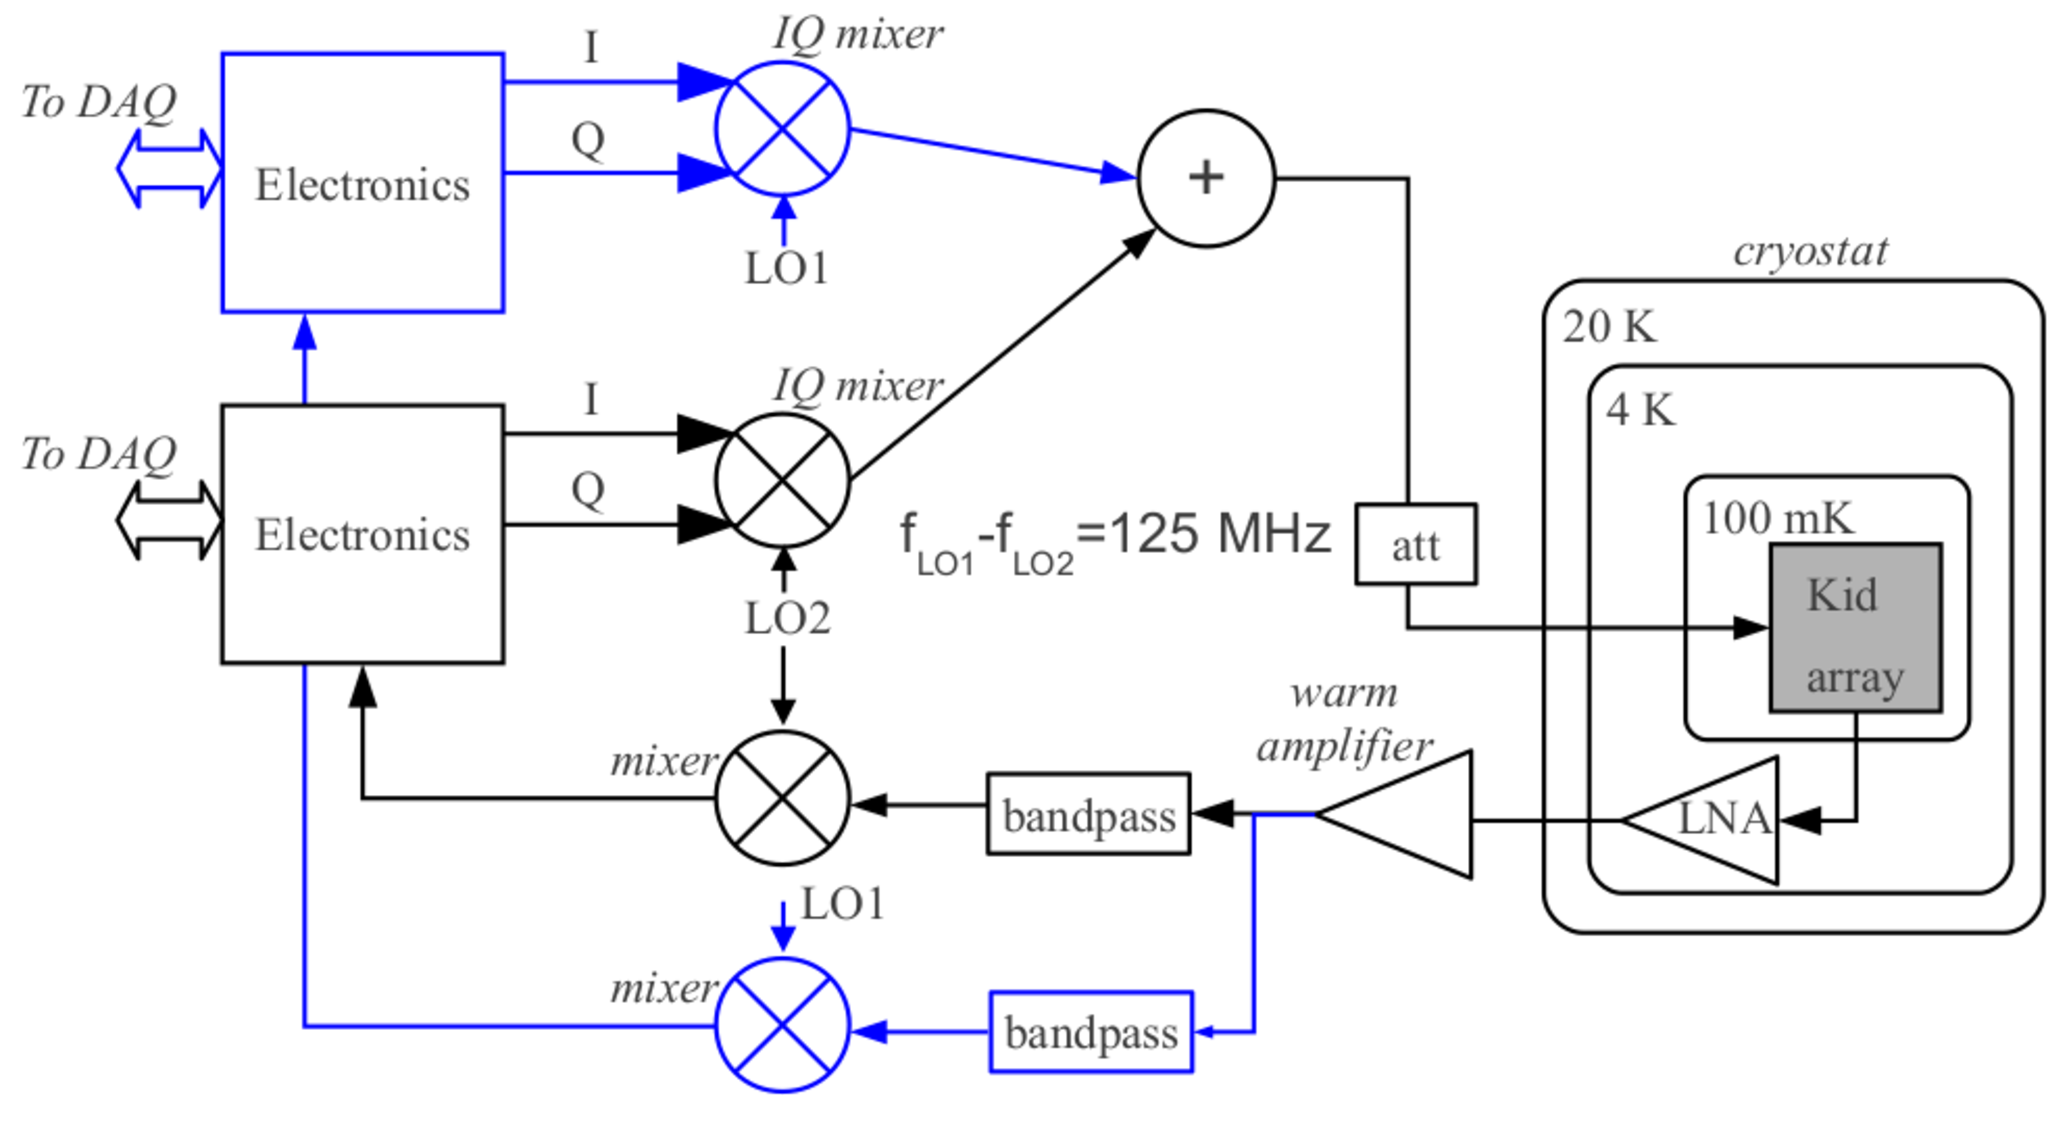
\includegraphics[width=0.5\textwidth]{nikel_readout}}
				\end{center}
								\begin{center}
												\only<2>{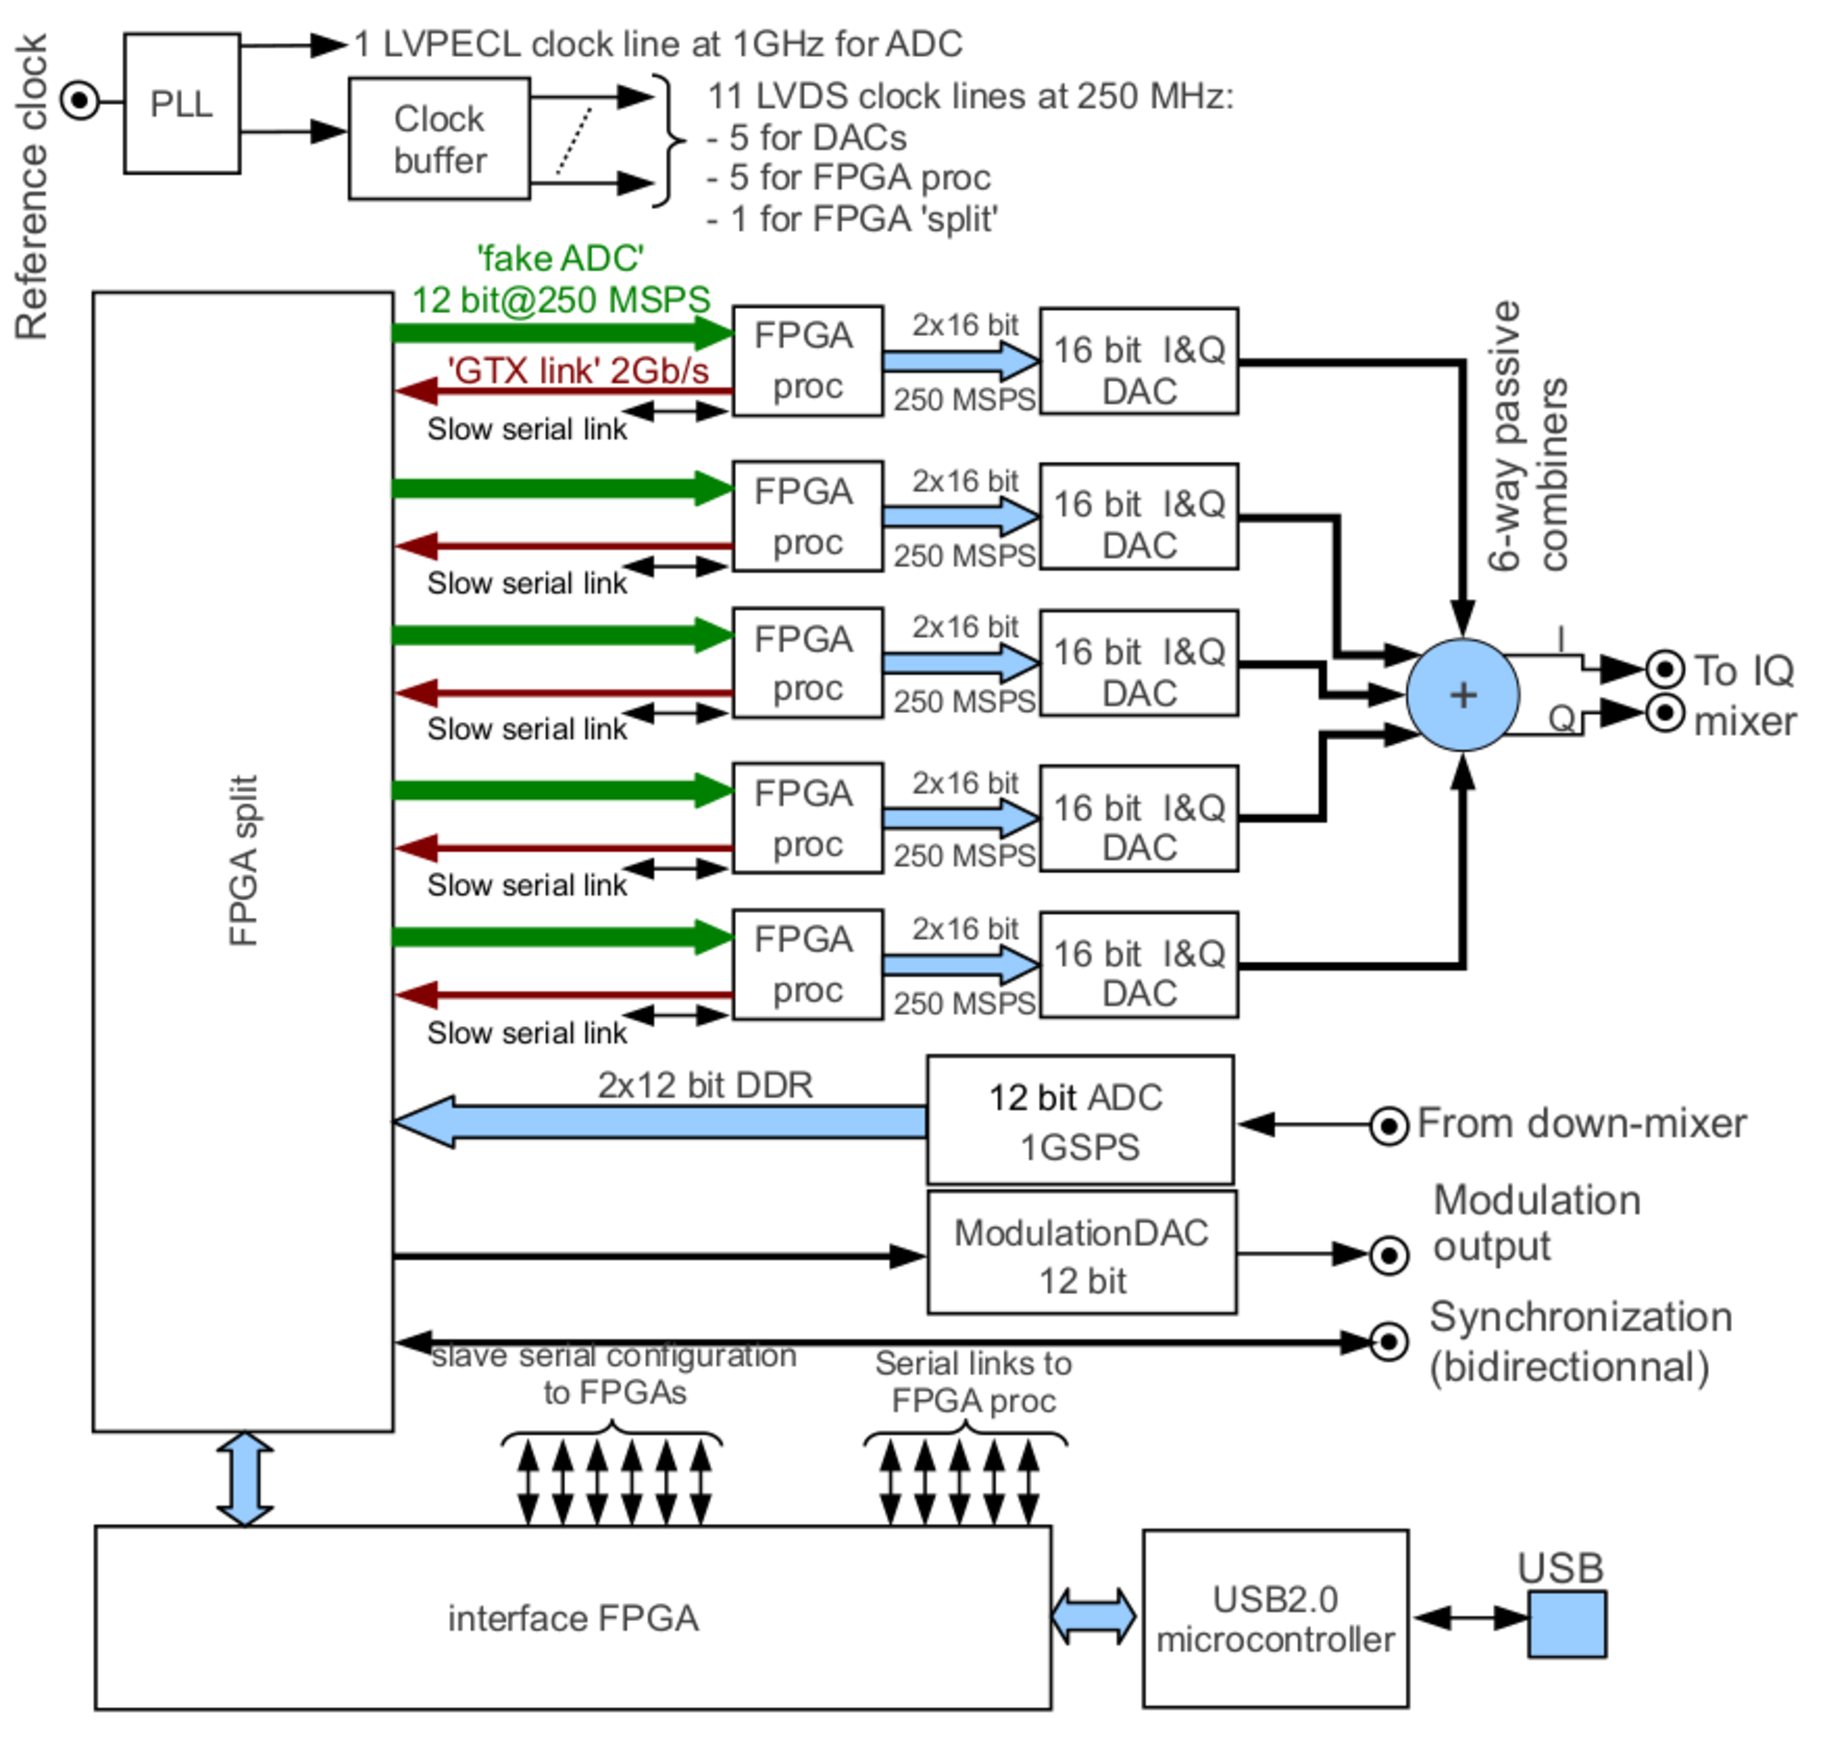
\includegraphics[width=0.5\textwidth]{nikel_readout2}}
												\only<2>{\includegraphics[width=0.5\textwidth]{nikel_readout3}}
								\end{center}
\end{frame}

\begin{frame}{Channelizer operación básica}
				\begin{center}
								\only<1>{\includegraphics[width=0.6\textwidth]{PFB_distribution_modulators}}
				\end{center}
								\begin{center}
												\only<2>{\includegraphics[width=0.8\textwidth]{PFB_final_arquitecture}}
								\end{center}
\end{frame}

\section{Vivado}
\begin{frame}{Vivado}

				Actualmente trabajando con la versi\'on 2016.4

				Cores propios, ej. RxChannelizer y TxChannelizer, etc.

				Mezcla de scripts TCL y Linux embebido
				\begin{center}
								\includegraphics[width=0.8\textwidth]{pfb_repo}
				\end{center}
\end{frame}

\begin{frame}{Proyectos Vivado}

				%\begin{columns}
				%\begin{column}{0.45\textwidth}
				\begin{center}
								\only<1>{\includegraphics[width=0.95\textwidth]{rxchan16_test2_vivado_project}}
				\end{center}
				%\end{column}
				%\begin{column}{0.45\textwidth}
								\begin{center}
												\only<2>{\includegraphics[width=0.8\textwidth]{channelizer16_core}}
								\end{center}
								%\end{column}
								%\end{columns}
\end{frame}

\section{Amplificador de bajo ruido}
\begin{frame}{Amplificador}
				\begin{columns}
								\begin{column}{0.45\textwidth}
												\includegraphics[angle=-90,width=0.62\textwidth]{amp_low_temp1} \\ 
												\includegraphics[angle=-90,width=0.6\textwidth]{sim900_mainframe_med_temp}
								\end{column}
								\begin{column}{0.45\textwidth}
												\includegraphics[angle=-90,width=0.62\textwidth]{acople_linea_mkid} \\ 
												\includegraphics[angle=-90,width=0.6\textwidth]{criostato_modelo}
								\end{column}
				\end{columns}
\end{frame}
\begin{frame}{Amplificador}
				\begin{columns}
								\begin{column}{0.45\textwidth}
												\includegraphics[angle=-90,width=0.62\textwidth]{mkid1} \\ 
												\includegraphics[angle=-90,width=0.6\textwidth]{mkid2}
								\end{column}
								\begin{column}{0.45\textwidth}
												\includegraphics[angle=-90,width=0.62\textwidth]{mkid3_magnetic_case} \\ 
												\includegraphics[angle=-90,width=0.6\textwidth]{mkid4}
								\end{column}
				\end{columns}
\end{frame}

\section{Amplificador de bajo ruido}
\begin{frame}{Amplificador}
				\begin{columns}
								\begin{column}{0.45\textwidth}
												\includegraphics[angle=-90,width=0.62\textwidth]{amp_low_temp1} \\ 
												\includegraphics[angle=-90,width=0.6\textwidth]{sim900_mainframe_med_temp}
								\end{column}
								\begin{column}{0.45\textwidth}
												\includegraphics[angle=-90,width=0.62\textwidth]{acople_linea_mkid} \\ 
												\includegraphics[angle=-90,width=0.6\textwidth]{criostato_modelo}
								\end{column}
				\end{columns}
\end{frame}
\section{Equipamiento BT}
Using section and subsection commands, outside of frames, provides a table of contents and progress information to beamer.
\begin{frame}{Equipos BT}
				\begin{columns}
								\begin{column}{0.45\textwidth}
												\includegraphics[angle=-90,width=0.62\textwidth]{IMG_20190523_105037648} \\ 
												\includegraphics[angle=-90,width=0.6\textwidth]{IMG_20190523_105054061}
								\end{column}
								\begin{column}{0.45\textwidth}
												\includegraphics[angle=-90, width=0.62\textwidth]{IMG_20190523_105443289} \\ 
												\includegraphics[angle=-90,width=0.6\textwidth]{IMG_20190523_105117465}
								\end{column}
				\end{columns}


				%				Aim for five to ten slides for a 25~minute presentation.
				%
				%				Certainly no more than 15.
				%
				%				Use a note form for the content of each slide.
				%
				%				\begin{theorem}
				%								Mathematics works within the Beamer class, $\exp(i\pi)+1=0$\,, including theorems.
				%				\end{theorem}
				%
				%				Click: \url{http://www.maths.adelaide.edu.au} 
\end{frame}

\begin{frame}{Equipos BT}
				\begin{columns}
								\begin{column}{0.45\textwidth}
												\includegraphics[angle=-90,width=0.62\textwidth]{IMG_20190523_111114131} \\ 
												\includegraphics[angle=-90,width=0.6\textwidth]{IMG_20190523_105054061}
								\end{column}
								\begin{column}{0.45\textwidth}
												\includegraphics[angle=-90,width=0.42\textwidth]{IMG_20190523_105647049} \\ 
												\hspace{2mm}\includegraphics[angle=-90,width=0.42\textwidth]{IMG_20190523_112752228} \\
												\includegraphics[angle=-90,width=0.42\textwidth]{IMG_20190523_104038976}
								\end{column}
				\end{columns}
				%				Aim for five to ten slides for a 25~minute presentation.
				%
				%				Certainly no more than 15.
				%
				%				Use a note form for the content of each slide.
				%
				%				\begin{theorem}
				%								Mathematics works within the Beamer class, $\exp(i\pi)+1=0$\,, including theorems.
				%				\end{theorem}
				%
				%				Click: \url{http://www.maths.adelaide.edu.au} 
\end{frame}

				\begin{frame}{Amplificador criog\'enico de bajo ruido}
								\framesubtitle{LNF-LNC03\_14A}
								\begin{columns}
												\begin{column}{0.40\textwidth}
																\hspace{10mm}\includegraphics[width=0.95\textwidth]{lnf-lnc03_14sa}
												\end{column}
												\begin{column}{0.60\textwidth}
																\begin{itemize}
																				\item Ancho de Banda RF: 0.3-14 GHz
																				\item Ruido: 4.1 K (típico)
																				\item Ganancia: 42 dB
																				\item Potencia DC: Vc= 0.7 V @ 14 mA
																				\item Conectores RF: G3PO Macho
																				\item Conector DC: Nano Strip 5 pines hembra
																\end{itemize}
												\end{column}
								\end{columns}
				\end{frame}

				%------------------------------------------------------------------------------
\section{Hardware}
\subsection{ZCU111 Ev. Kit}%es el diseño de Israel
\begin{frame}{Kit de evaluación ZCU111}
				\centering
												\includegraphics[width=0.4\textwidth]{isra_mkid1}
												\includegraphics[width=0.32\textwidth]{isra_mkid2}
\end{frame}
\begin{frame}{Barrido en potencia}
				\centering
												\includegraphics[width=0.4\textwidth]{isra_mkid3}
												\includegraphics[width=0.32\textwidth]{isra_mkid4}
\end{frame}
\begin{frame}{Barrido en potencia}
				\centering
												\includegraphics[width=0.4\textwidth]{isra_mkid1}
												\includegraphics[width=0.32\textwidth]{isra_mkid2}
\end{frame}


%------------------------------------------------------------------------------
\section{Mediciones}
\subsection{Diseño FNAL}%es el diseño de Israel
\begin{frame}{Barrido en potencia}
				\centering
												\includegraphics[width=0.4\textwidth]{isra_mkid1}
												\includegraphics[width=0.32\textwidth]{isra_mkid2}
\end{frame}
\begin{frame}{Barrido en potencia}
				\centering
												\includegraphics[width=0.4\textwidth]{isra_mkid3}
												\includegraphics[width=0.32\textwidth]{isra_mkid4}
\end{frame}
\begin{frame}{Barrido en potencia}
				\centering
												\includegraphics[width=0.4\textwidth]{isra_mkid1}
												\includegraphics[width=0.32\textwidth]{isra_mkid2}
\end{frame}
\subsection{Diseño UCSB}
\begin{frame}{Diseño de la Universidad de California, Santa Bárbara (UCSB)}
				\framesubtitle{Características}
				\begin{columns}
								\begin{column}{0.49\textwidth}
												\includegraphics[width=0.4\textwidth]{mkid4}
												\begin{itemize}
																\item[o] Arreglo utilizado en ARCONS (Array
																				Camera for Optical to Near-IR
																				Spectrophotometry)
																\item[o] Arreglo de 44 x 46 resonadores (\alert{2024
																				píxeles})
																\item[o] Separación entre frecuencias de
																				resonancia $\to$ \alert{2 MHz}
																\item[o] Nitrato de Titanio con una temperatura
																				crítica de \alert{$\sim$ 0.9 K}
																\item[o] Banda de observación: \alert{380 nm --
																				1150 nm}
												\end{itemize}
								\end{column}
								\begin{column}{0.49\textwidth}
												\centering
												\includegraphics[angle=-90,width=0.72\textwidth]{mkid2}
								\end{column}
				\end{columns}
\end{frame}
\begin{frame}{Diseño de la Universidad de California, Santa Bárbara (UCSB)}
				\framesubtitle{Características}
				\begin{columns}
								\begin{column}{0.49\textwidth}
												\only<1>{\includegraphics[width=0.4\textwidth]{mkid4}}
												\begin{itemize}
																\item[o] TiN sobre Si
																\item[o] TiN de 60 nm
																\item[o] Wire bonds de oro a los pads para
																				disipación de calor
																\item[o] Caja de cobre enchapada en oro (solo
																				materiales no magnéticos)
																\item[o] Wire bonds de Al a las líneas
																				de Tx

																				%	Las pestañas sostienen el chip hacia
																				%	abajo y ayudan a aplastar el pegamento
																				%	para que el chip quede al ras del brazo.
												\end{itemize}
								\end{column}
								\begin{column}{0.49\textwidth}
												\centering
												%\only<1>{\includegraphics[width=0.5\textwidth]{mkid4}}
												\only<1>{\includegraphics[angle=-90,width=0.72\textwidth]{mkid2}}
												\only<2>{\includegraphics[width=0.82\textwidth]{mkid5}}
												\only<2>{\includegraphics[width=0.82\textwidth]{mkid6}}
												\only<3>{\includegraphics[width=0.82\textwidth]{mkid7}}
												\only<3>{\includegraphics[width=0.82\textwidth]{mkid8}}
								\end{column}
				\end{columns}
\end{frame}
\begin{frame}{Diseño de la Universidad de California, Santa Bárbara (UCSB)}
				\framesubtitle{Características}
				\centering
								%				\includegraphics[width=0.42\textwidth]{resonador0_asc_sin_filtro}
												\includegraphics[width=0.62\textwidth]{mkid_ucsb1}
\end{frame}
\begin{frame}{Diseño de la Universidad de California, Santa Bárbara (UCSB)}
				\framesubtitle{Características (Charla de Donna Kubik, FNAL)}
				
				\centering
								%				\includegraphics[width=0.42\textwidth]{resonador0_asc_sin_filtro}
												\includegraphics[width=0.72\textwidth]{mkid_ucsb2}
\end{frame}
\begin{frame}{Estudio de la $T_c$}
				\only<1>{\begin{equation*}
								\frac{\sigma_2(T)}{\sigma_N} \simeq
																\frac{\pi \Delta}{\hbar
																\omega}\left[1-2\exp \left(-\frac{\Delta}{k_B
																T}\right)\exp \left(-\frac{\hbar \omega}{2 
																k_B T}\right)
																I_0 \left(\frac{\hbar \omega}{2 k_B T}\right)\right]
				\end{equation*}}
				\only<2>{Resultados en concordancia a los medidos en la UCSB en todo el arreglo}
				\centering
												\only<1>{\includegraphics[width=0.82\textwidth]{delta_f_vs_temp}}
												\only<2>{\includegraphics[width=0.56\textwidth]{delta_f_vs_temp}}
												\only<2>{\includegraphics[width=0.42\textwidth]{medicion_Tc_ucsb}}
\end{frame}
\begin{frame}{Barrido en potencia}
				\begin{itemize}
								\item[*] -25 dB hasta -50 dB + atenuador de 30 dB
				\end{itemize}
				\centering
												\includegraphics[width=0.48\textwidth]{resonador0_asc_sin_filtro}
												\includegraphics[width=0.48\textwidth]{resonador0_asc_filtro}
\end{frame}
\begin{frame}{Barrido en potencia}
				\centering
								%				\includegraphics[width=0.42\textwidth]{resonador0_asc_sin_filtro}
												\includegraphics[width=0.82\textwidth]{resonador0_asc_filtro}
\end{frame}
\begin{frame}{Barrido en potencia}
				\begin{itemize}
								\item[*] -25 dB hasta -50 dB + atenuador de 30 dB
				\end{itemize}
				\centering
												\includegraphics[width=\textwidth]{res0_asc_full_potencias}
\end{frame}
\begin{frame}{Barrido en potencia}
				\begin{itemize}
								\item[*] -25 dB hasta -50 dB + atenuador de 30 dB
				\end{itemize}
				\centering
												\includegraphics[width=\textwidth]{res0_3_potencias}

\end{frame}
\begin{frame}{Barrido en potencia}
				\centering
												\includegraphics[width=0.82\textwidth]{res0_Q_vs_P}

\end{frame}
\begin{frame}{Q vs Potencia}
				\begin{columns}
								\begin{column}{0.49\textwidth}
												\qquad \qquad-55 dB $\to$ -80 dB

												\centering
												\includegraphics[height=0.50\textheight,width=1.1\textwidth]{Q_vs_P_tot_des}
								\end{column}
								\begin{column}{0.49\textwidth}
												-80 dB $\to$ -55 dB
												\centering
												\includegraphics[height=0.50\textheight,width=1.1\textwidth]{Q_vs_P_tot_asc}
								\end{column}
				\end{columns}

\end{frame}

\subsection{Diseño del filtro prototipo}
\begin{frame}{Arquitectura}
        \begin{center}
                \includegraphics[width=0.8\textwidth]{PFB_final_arquitecture}
        \end{center}
\end{frame}

\begin{frame}{Filtro PFB - Ch5 $f_\text{centro}= 512\,\text{MHz}$}
        \begin{center}
                \only<1>{\includegraphics[width=0.8\textwidth]{ch5_design}}
        \end{center}
        \vspace{-1.2cm}
        \begin{center}
                \only<2>{\includegraphics[width=0.8\textwidth]{ch5_out_456}}
        \end{center}
        \vspace{-1.8cm}
        \begin{columns}
                \begin{column}{0.5\textwidth}
        \begin{center}
                \only<3>{\includegraphics[width=\textwidth]{ch5_out_456}}
        \end{center}
                \end{column}
                \begin{column}{0.5\textwidth}
        \begin{center}
                \only<3>{\includegraphics[width=\textwidth]{ch5_design_zoom}}
        \end{center}
                \end{column}
        \end{columns}
        %\vspace{-.8cm}
        \begin{center}
                \only<4>{\includegraphics[width=\textwidth]{ch5_zoom_456}}
        \end{center}
\end{frame}
\begin{frame}{Ganancia del DAC en RFSoc}
        \begin{center}
                \includegraphics[width=0.8\textwidth]{dac_gain}
        \end{center}
\end{frame}

\section{Perspectivas de trabajo}
\begin{frame}{Perspectivas de trabajo}
				\begin{itemize}
								\item Dise\~no de resonador en Sonnet
								\item Primeras mediciones a $T_{amb}$ y $T \sim 100\,mK$
								\item Definici\'on de requerimientos para crio (cables,
												conectores, espacios, etc.)
								\item Primeras pruebas con RxChannelizer con ITeDA (pruebas de
												front-end, mezcladores, filtros, DC-block, etc.)
				\end{itemize}
\end{frame}
%\section{El algoritmo de Goertzel}
\begin{frame}{El algoritmo de Goertzel}
				\begin{itemize}
								\item Finalize performance requirements for firmware 
								\item Finalize performance requirements for Tx and Rx parts 
								\item First tests of RxChannelizer (front-end, mixers, filters,
												DC-block, etc.)
				\end{itemize}
								\centering
								\includegraphics[width=0.45\textwidth]{goertzel_algo}
\end{frame}

\begin{frame}{El algoritmo de Goertzel}
				\begin{itemize}
								\item Finalize performance requirements for firmware 
								\item Finalize performance requirements for Tx and Rx parts 
								\item First tests of RxChannelizer (front-end, mixers, filters,
												DC-block, etc.)
				\end{itemize}
								\centering
								\includegraphics[width=0.45\textwidth]{goertzel_non_integer_figure1}
\end{frame}

\section{Work perspectives}
\begin{frame}{Work perspectives}
				\begin{itemize}
								\item Finalize performance requirements for firmware 
								\item Finalize performance requirements for Tx and Rx parts 
								\item First tests of RxChannelizer (front-end, mixers, filters,
												DC-block, etc.)
				\end{itemize}
\end{frame}
%\section{Prefer titles that make a statement}
%\begin{frame}{Prefer titles that make a statement}
%
%				Many opt for meaningless titles and section titles.  
%
%				Instead, make titles convey information.
%
%				\pause
%
%				Use \texttt{pause} commands almost anywhere to progressively step through material.
%
%				\pause
%
%				\begin{figure}
%								\centering
%								\caption{Figure and table environments also work.
%								Use \texttt{includegraphics} or \texttt{pgfplots}.}
%								\begin{tikzpicture}
%												\begin{axis}[footnotesize,axis lines=middle
%																,xlabel={$t$},no marks,thick,domain=0:2.2,smooth ]
%																\addplot+[]{1-2*exp(-2*x)+exp(-4*x)};
%																\addlegendentry{$u(t)$};
%																\addplot+[]{1-exp(-4*x)};
%																\addlegendentry{$v(t)$};
%																\addplot+[]{1+2*exp(-2*x)+exp(-4*x)};
%																\addlegendentry{$w(t)$};
%												\end{axis}
%								\end{tikzpicture}
%				\end{figure}
%
%\end{frame}
%
%
%
%
%\section{Conclusion}
%\begin{frame}{Conclusion}
%
%				Finish with your conclusions displayed: \emph{not} a list of references, \emph{nor} a meaningless ``thank you'' slide.
%
%				\vfill
%				\begin{quote}
%								Three rules of public speaking: Be forthright.  Be brief.  Be
%								seated. \hfill(S. Dressel \& J. Chew, 1987)
%				\end{quote}
%\end{frame}




\end{document}

